\documentclass[twoside,openright,bibliography=totoc]{scrreprt}
%\documentclass[report,mono,twoside,openright]{tugrazbooklet}
%\documentclass[a4paper]{book}

\usepackage[phd]{tugrazthesis}
% options:
%   - msc (for Master's thesis/Masterarbeit) OR
%     diplom (for Diploma thesis/Diplomarbeit) OR
%     phd (for Doctoral thesis/Dissertation)
%   - nawi (for NAWI curricula)
%   - individual (for Individuelles Masterstudium)

\usepackage[ngerman,british]{babel}  % uncomment to switch to German

%\usepackage{filecontents}  % for the integrated bibliography file (backwards compatibility)
%\usepackage[backend=backend,style=numeric-comp]{biblatex}  % to generate the bibliography
%\addbibresource{phd-missethan.bib}  % name of the bib-file

%---Packages-Introduction---------------------------------------------------------------

\usepackage[sort]{cite}
\usepackage{amsmath,amssymb,amsthm}
\definecolor{colourCite}{RGB}{50,128,50}
\definecolor{colourLink}{RGB}{200,0,0}
\usepackage[citebordercolor=colourCite,linkbordercolor=colourLink]{hyperref}
\usepackage[capitalize, noabbrev]{cleveref}


% ---------------- Theorem environments ---------------------------------

\newtheorem{theorem}{Theorem}[section]
\newtheorem{proposition}[theorem]{Proposition}
\newtheorem{corollary}[theorem]{Corollary}
\newtheorem{lemma}[theorem]{Lemma}
\newtheorem{observation}[theorem]{Observation}
\newtheorem{conjecture}[theorem]{Conjecture}
\newtheorem{prob}{Problem}[]
\theoremstyle{definition} 
\newtheorem{definition}[theorem]{Definition}
\newtheorem{example}[theorem]{Example}
\newtheorem{question}[theorem]{Question}

\crefname{theorem}{theorem}{theorems}
\crefname{proposition}{proposition}{propositions}
\crefname{corollary}{corollary}{corollaries}
\crefname{lemma}{lemma}{lemmas}
\crefname{definition}{definition}{definitions}
\crefname{conjecture}{conjecture}{conjectures}


%--------------- Chapter 1. Recoverable Selection
%\usepackage{natbib}
%\usepackage{etex}
%\usepackage{scrhack}
%\usepackage{cmap}
%\usepackage[ngerman,english]{babel}
\usepackage[utf8]{inputenc}
\usepackage{graphicx}
\usepackage{caption}
\usepackage{subfigure}
%\usepackage{epstopdf}
\usepackage{mathtools}
%\usepackage{amsmath}
%\usepackage{amsthm}
%\usepackage{amssymb}
%\usepackage{comment}
\usepackage{multirow}
\usepackage{tikz}
%\usetikzlibrary{arrows,intersections}
%\usetikzlibrary{shapes}
%\usepackage[english,vlined,ruled]{algorithm2e}
\usepackage{hyperref}
\usepackage{lipsum}
\usepackage{float}
\usepackage{tabularx}
%\usepackage{booktabs}
%\usepackage{longtable}
%\usepackage{tabu}
%\usepackage{environ}
%\usepackage{mdframed}
%\usepackage{datetime}
\usepackage{enumerate}
%\usepackage{authblk}

%%------------------------ Chapter 3. Interval Interdiction
%\usepackage{amsmath}
%\usepackage{amsfonts}
%\usepackage{amssymb}
\usepackage{authblk}

%\usepackage{graphicx}
%\usepackage{hyperref}
%\usepackage[capitalize, noabbrev]{cleveref}
\usepackage[autostyle=true]{csquotes}
\usepackage{color}
\usepackage{multirow}
%algorithm package
\usepackage[ruled, lined, linesnumbered, commentsnumbered, noend]{algorithm2e}
%packages used for subfigures
%\usepackage{caption}
%\usepackage{subcaption}

%%--------------------------- Chapter 5. Linearization 2

%\usepackage[utf8]{inputenc}
%\usepackage{amsmath}
%\usepackage{amsfonts}
%\usepackage{amssymb}
%\usepackage{authblk}
\usepackage{verbatim}
\usepackage{thmtools}
%\usepackage{amsthm}
\usepackage{thm-restate}
\usepackage{todonotes}
%\declaretheorem[name=Theorem,numberwithin=section]{thm}
%--experiment
%\usepackage%[hidelinks]{hyperref}

%\usepackage[capitalize, noabbrev]{cleveref}
%\usepackage[autostyle=true]{csquotes}
%\usepackage{graphicx}
%\usepackage{color}
%\usepackage{enumerate}
%\usepackage[ruled, lined, linesnumbered, commentsnumbered, noend]{algorithm2e}

%\usepackage{tikz}
\usetikzlibrary{calc}
\usetikzlibrary{arrows,shapes}
\usetikzlibrary{decorations.markings}
\usetikzlibrary{arrows.meta}

%------------------------ Chapter 6. Nonpreemptive Tree Packing

%\usepackage[utf8]{inputenc}
%\usepackage{amsmath,amsfonts,amssymb}
%\usepackage{thmtools}
%\usepackage{amsthm}
%\usepackage{thm-restate}

%\usepackage{hyperref}
%\usepackage[capitalize, noabbrev]{cleveref}
%\usepackage{graphicx}
%\usepackage{color}
%\usepackage{enumerate}
%\usepackage{caption}
%\usepackage{subcaption}
\usepackage{array}
%\usepackage{authblk}

\usepackage{tikz,tikzsymbols}
\usetikzlibrary{shapes,patterns,positioning}
\usetikzlibrary{arrows,decorations.markings}
\usetikzlibrary{calc}


\makeatletter
\renewcommand{\@pnumwidth}{3em} 
\renewcommand{\@tocrmarg}{4em}
\makeatother

\overfullrule=3mm


\newtheorem{thm}{Theorem}[section]
\newtheorem{prop}[thm]{Proposition}
\newtheorem{coro}[thm]{Corollary}
\newtheorem{lem}[thm]{Lemma}
\newtheorem{conjecture}[thm]{Conjecture}
\theoremstyle{remark}
\newtheorem{remark}[thm]{Remark}
\theoremstyle{definition}
\newtheorem{definition}[thm]{Definition}

\crefname{thm}{theorem}{theorems}
\crefname{prop}{proposition}{propositions}
\crefname{coro}{corollary}{corollaries}
\crefname{lem}{lemma}{lemmas}
\crefname{definition}{definition}{definitions}
\crefname{conjecture}{conjecture}{conjectures}

\renewcommand{\theenumi}{\normalfont(\roman{enumi})}
\renewcommand{\labelenumi}{\theenumi}


\newtheoremstyle{claim}%name
{}%Space above
{}%Space below
{\itshape}%Body font
{}%Indent amount
{\bfseries}%Theorem head font
{.}%Punctuation after theorem head
{0.5em}%Space after theorem head
{}%Theorem head spec(can be left empty, meaning ‘normal’)
\theoremstyle{claim}
\newtheorem{claim}{Claim}

\crefname{claim}{claim}{claims}

%---Macros-Universal---------------------------------------------------------------
\newcommand{\R}{\mathbb{R}}
\newcommand{\N}{\mathbb{N}}
\newcommand{\Z}{\mathbb{Z}}
\newcommand{\set}[1]{\{ #1 \}}
\newcommand{\fromto}[2]{\set{#1, \ldots, #2}}

\newcommand{\rz}{\mathbb{R}}
\newcommand{\nz}{\mathbb{Z}}


\newcommand{\bigO}{\mathcal{O}}
\newcommand{\dotunion}{\mathbin{\dot{\cup}}}
\newcommand{\powerset}{\mathcal{P}}



%---------- Chapter 1. Recoverable Selection -------------
\newcommand{\bigM}{\Omega}
\newcommand{\ra}{\rightarrow}
\newcommand{\la}{\leftarrow}
\newcommand{\Ra}{\Rightarrow}
\newcommand{\La}{\Leftarrow}
\newcommand{\sgn}{\operatorname{sgn}}
\newcommand{\out}{\operatorname{out}}
\newcommand{\inn}{\operatorname{in}}
\newcommand{\val}{\operatorname{val}}
\newcommand{\head}{\operatorname{head}}
\newcommand{\tail}{\operatorname{tail}}
\newcommand{\rev}{\operatorname{rev}}
\newcommand{\ord}{\operatorname{ord}}
\newcommand{\prev}{\operatorname{prev}}
\newcommand{\first}{\operatorname{first}}
\newcommand{\last}{\operatorname{last}}
\newcommand{\oleft}{\operatorname{left}}
\newcommand{\aux}{\operatorname{aux}}
\newcommand{\mh}{displaymath}
\newcommand{\nn}{\mathbb{N}}
\newcommand{\nnz}{\mathbb{N}_0}
\newcommand{\qq}{\mathbb{Q}}
\newcommand{\zz}{\mathbb{Z}}
\newcommand{\rr}{\mathbb{R}}
\newcommand{\kk}{\mathbb{K}}
\newcommand{\cc}{\mathbb{C}}
\newcommand{\ff}{\mathbb{F}}
\newcommand{\pp}{\mathcal{P}}
\newcommand{\eps}{\epsilon}
\newcommand{\Lra}{\Leftrightarrow}
\newcommand{\mbf}[1]{\text{\textbf{#1}}}
\newcommand{\udot}{\mathbin{\dot{\cup}}}
\newcommand{\bigudot}{\mathop{\dot{\bigcup}}}
\newcommand{\vek}[1]{\boldsymbol{#1}}
\newcommand{\id}{\operatorname{id}}
\newcommand{\poly}{\operatorname{poly}}
\newcommand{\scalp}[2]{{#1}^{t} {#2}}
\newcommand{\method}[1]{\texttt{#1}}
\newcommand{\opt}{\mathit{OPT}}
\newcommand{\alg}{\mathit{ALG}}
\newcommand{\rank}{\operatorname{rk}}
\newcommand{\probl}[1]{\textsc{#1}}
\newcommand{\matroid}{\mathcal{M}}
\newcommand{\base}{E}
\newcommand{\basis}{\mathcal{B}}
\newcommand{\inds}{\mathcal{F}}
\newcommand{\transit}{\tau}
\newcommand{\myc}{c}
\newcommand{\myd}{\bar{c}}
\newcommand{\scenset}{\mathcal{U}}
\newcommand{\lowcost}{\underline{c}}
\newcommand{\upcost}{\bar{c}}
\newcommand{\fscost}{C}

\newcommand{\X}{\mathcal{X}}
\newcommand{\cU}{\mathcal{U}}

\newcommand{\fillfield}[2]{\draw[fill=lightgray]  (#1-1,#2-1,0) -- (#1-1,#2,0) -- (#1,#2,0) -- (#1,#2-1,0) -- cycle;}
\newcommand{\fillfieldr}[2]{ \draw[step=1,thick, red] (#1-1,#2-1) grid (#1,#2); }
\newcommand{\fillfieldg}[2]{ \draw[step=1,thick, blue] (#1-1,#2-1) grid (#1,#2); }

% names
\newcommand{\ptime}[2]{p^{(#1)}_{#2}}
\newcommand{\plow}[1]{p^{-}_{#1}}
\newcommand{\pup}[1]{p^{+}_{#1}}
\newcommand{\ctime}[2]{C^{(#1)}_{#2}}

\newcommand{\lasse}[1]{{#1}}

\DeclareMathOperator*{\argmax}{\arg\!\max}
\DeclareMathOperator*{\argmin}{\arg\!\min}

\DeclarePairedDelimiter{\ceil}{\lceil}{\rceil}
\DeclarePairedDelimiter{\floor}{\lfloor}{\rfloor}
\DeclarePairedDelimiter{\abs}{\lvert}{\rvert}


%------------ Chapter 2. Multistage Complexity

\newcommand{\new}[1]{#1}
%\newcommand{\X}{{\mathcal{X}}}
%\newcommand{\cU}{{\mathcal{U}}}
\newcommand{\cI}{{\mathcal{I}}}
\newcommand{\cC}{{\mathcal{C}}}
\newcommand{\cB}{{\mathcal{B}}}
%\newcommand{\rev}[1]{\textcolor{blue}{#1}} %text segments changed in the revision
%\newcommand{\R}{\mathbb{R}}
%\newcommand{\N}{\mathbb{N}}

\newcommand{\radj}{R-Adj-SAT}

\newcommand{\unc}{\mathcal{Z}}

%\newcommand{\set}[1]{\{ #1 \}}
%\newcommand{\fromto}[2]{\set{#1,\dots,#2}}

%------------ chapter 3. Interval Interdiction

\newcommand{\True}{\textsc{True}}
\newcommand{\False}{\textsc{False}}

%\newcommand{\comment}[1]{\textcolor{red}{(#1)}}

\newcommand{\las}[1]{#1}

\newcommand{\hun}[1]{#1}

\DeclareMathOperator{\ac}{\text{A}}
%\DeclareMathOperator{\val}{\text{value}}
\DeclareMathOperator{\dist}{\text{dist}}
\DeclareMathOperator{\rel}{\text{rel}}
\DeclareMathOperator{\betw}{\text{betw}}
\DeclareMathOperator{\valid}{\text{valid}}
\DeclareMathOperator{\cost}{\text{cost}}



%Special short commands for interval interdiction notation
\newcommand{\I}{\mathcal{I}}
\newcommand{\J}{\mathcal{J}}
\newcommand{\F}{\mathcal{F}}
\DeclareMathOperator{\graph}{G}

\newcommand{\claimqed}{\hfill\scriptsize$\blacksquare$\normalsize}

%---------------- Chapter 4. Linearization 1

%\newcommand{\proof}{\emph{Proof.}\ \ }
%\newcommand{\qed}{~~$\Box$}
\newcommand{\RRR}{{\mathbb{R}_{\ge0}}}

\newcommand{\spp}{\text{SPP}}
\newcommand{\qspp}{\text{QSPP}}
\newcommand{\ppp}{{\cal P}_{st}}
\newcommand{\pppx}{{\cal P}^+}
\newcommand{\pppy}{{\cal P}^-}

\newcommand{\boxxx}[1]
 {\fbox{\begin{minipage}{13.00cm}\begin{center}\bigskip\begin{minipage}{12.30cm}
  #1\end{minipage}\end{center}~\end{minipage}}}

%---------------- Chapter 5. Linearization 2


\newcommand{\const}{\textsf{source}}
%\newcommand{\ren}[1]{{\color{magenta}{#1}}}

\newcommand{\Pst}{\mathcal{P}_{st}}
\newcommand{\Nscript}{N}

%\newcommand{\boxxx}[1]
% {\fbox{\begin{minipage}{11.80cm}\begin{center}\bigskip\begin{minipage}{11.30cm}
%  #1\end{minipage}\end{center}~\end{minipage}}}

\DeclareMathOperator{\red}{\textsf{reduced}}
\DeclareMathOperator{\xval}{val}

%----------------------- Chapter 6. NTP

\newcommand{\RR}{\mathbb{R}}
\newcommand{\NN}{\mathbb{N}}
\newcommand{\ZZ}{\mathbb{Z}}

%\newcommand{\comment}[1]{\textcolor{red}{(L: #1)}}

\newcommand{\xxxNTP}{\textsc{N-TreePack}}
\newcommand{\xxxHAM}{\textsc{Hamilton-3-reg}}
\DeclareMathOperator{\ntp}{\textsf{ntp}}
\newcommand{\greedy}{\textsf{Greedy}}

%\newcommand{\lasse}[1]{\textcolor{blue}{#1}}
%\newcommand{\lasse}[1]{#1}



\newcommand{\creflastconjunction}{, and\nobreakspace}

\begin{document}
%--- INFORMATION FOR TITLEPAGE -------------------------------------------------

% Your name including previous academic degrees (optional argument sets a different \author{}):
\thesisauthor[Michael Missethan]{Dipl.-Ing. Michael Missethan, BSc}

% Title of your thesis (optional argument sets a different \title{}):
\thesistitle[Random planar graphs]{Global and local properties\\of random planar graphs}

% Date of completion (optional argument sets a different \date{})
\thesisdate[ ]{February 2022}

% Supervisor headline (select male/female/plural version)
\supervisortitle{\germanenglish{Betreuerin/Betreuer}{Supervisor}}

% Supervisor info
\supervisor{%
  Univ.-Prof. Mihyun Kang, Ph.D.
\\[0.7cm]
  Institute of Discrete Mathematics

  %optional extra information (second advisor, name of faculty, etc.)\\
  %up to 2 lines
}

% Academic degree achieved with this thesis, according to your curriculum (check curriculum and select male/female version):
\academicdegree{Doktor der technischen Wissenschaften} % phd


%--- FRONT MATTER --------------------------------------------------------------
\pagenumbering{gobble}


% Insert title page and affidavit

\printthesistitle

\printaffidavit

% Other front matter you may want to include

\pagenumbering{roman}

\chapter*{Abstract}

In this thesis we study the asymptotic behaviour of the {\em uniform random planar graph}, which is a graph chosen uniformly at random from the class of all planar graphs with given number of vertices and edges. We mainly focus on the sparse regime when the average degree is at most two where it is known that many global and local structures and graph parameters of a uniform random planar graph undergo sudden changes, such as the component structure and the order of the largest component.

We provide various results on the {\em global structure} of a uniform random planar graph, such as asymptotic bounds on the length of the longest and shortest cycle and the number of vertices in its largest block. We also determine the asymptotic number of cut vertices in a uniform random planar graph and show that its maximum degree takes quite likely only one of two values. Furthermore, we describe the typical {\em local structure} of a uniform random planar graph around a randomly chosen vertex. In comparison to the classical \ER\ random graph, our results show that a uniform random planar graph exhibits very different behaviour in global and local properties and graph parameters studied in this thesis.

The key proof methods include combinatorial counting techniques, such as the so-called {\em core-kernel approach}, and probabilistic approaches, such as the P\'olya urn model and the second moment method. The core-kernel approach is based on a piecewise construction of graphs via substructures, called kernels and cores. Using it, we find useful relations between a uniform random planar graph and very classical random experiments, such as the balls-into-bins model.

Apart from a uniform random planar graph, we investigate the {\em random planar graph process}, in which we check edges one after another, accept an edge only if its addition to the current graph keeps the planarity of the resulting graph, and discard it otherwise. We derive the asymptotic number of accepted edges and the number of vertices in the largest component in the random planar graph process.

We also extend our results to a much more general class of graphs than planar graphs, including series-parallel graphs and graphs on a surface.


\begin{otherlanguage}{ngerman}
\chapter*{Kurzfassung}
In dieser Arbeit behandeln wir das asymptotische Verhalten des {\em planaren Zufallsgraphen}, welcher gleichverteilt auf der Klasse aller planaren Graphen mit gegebener Anzahl an Knoten und Kanten ist. Der Schwerpunkt liegt dabei auf dem so genannten dünn besetzten Bereich, in welchem der durchschnittliche Knotengrad höchstens zwei ist. Es ist allgemein bekannt, dass sich in diesem Bereich viele globale und lokale Eigenschaften des planaren Zufallsgraphen abrupt ändern, wie zum Beispiel die Struktur der Zusammenhangskomponenten oder die Anzahl der Knoten in der größten Zusammenhangskomponente. 

Wir betrachten zahlreiche weitere {\em globale Eigenschaften} des planaren Zufallsgraphen und erarbeiten asymptotische Schranken für die Länge des längsten und kürzesten Kreises sowie für die Anzahl der Knoten im größten Block. Darüber hinaus bestimmen wir die asymptotische Anzahl an Gelenkpunkten im planaren Zufallsgraphen und zeigen, dass der maximale Knotengrad üblicherweise einen von nur zwei möglichen Werten annimmt. Des Weiteren beschreiben wir die {\em lokale Struktur} des planaren Zufallsgraphen in der Nähe eines zufällig gewählten Knotens. Unsere Resultate zeigen sehr deutlich, wie sich das Verhalten des planaren Zufallsgraphen von jenem des klassischen \ER\ Zufallsgraphen unterscheidet. 

Unsere Beweisführung basiert auf kombinatorischen Abzählargumenten, wie zum Beispiel der so genannten {\em Core-Kernel-Methode}, und probabilistischen Ansätzen, wie zum Beispiel P\'olyas Urne und der Momenten-Methode. Bei der Core-Kernel-Methode werden Graphen mit Hilfe von Unterstrukturen, welche auch Cores und Kernels genannt werden, stückweise konstruiert. Unter Verwendung dieser finden wir nützliche Zusammenhänge zwischen dem planaren Zufallsgraphen und klassischen Zufallsexperimenten, wie zum Beispiel die zufällige Aufteilung von Bällen auf Fächer.

Neben dem planaren Zufallsgraphen betrachten wir auch den {\em planaren Zufallsgraphen-Prozess}, bei welchem wir mit einem Graphen ohne Kanten starten. Danach wählen wir in jedem Schritt zufällig eine mögliche Kante aus und fügen sie hinzu, wenn der Graph planar bleibt. Andernfalls verwerfen wir die Kante und betrachten sie danach nicht mehr. Wir bestimmen die asymptotische Anzahl der akzeptierten Kanten sowie die Anzahl der Knoten in der größten Zusammenhangskomponente im Laufe des planaren Zufallsgraphen-Prozesses.

Wir verallgemeinern unsere Resultate auch auf zahlreiche weitere Klassen von Graphen, unter anderem seriell-parallele Graphen und Graphen auf Oberflächen.
\end{otherlanguage}



% You will typically include *both a German and an English abstract*.
% The rest of the document will be either in German or in English.

\cleardoublepage

\chapter*{\germanenglish{Danksagung}{Acknowledgements}}

I would like to thank my supervisor Mihyun Kang for her constant support and discussions
throughout my Ph.D. studies and many helpful comments and suggestions for my thesis. She introduced me to the world of random graphs and her enthusiasm for this field impressed me time and again. I also thank my colleagues at the Institute of Discrete Mathematics for having been kind and friendly companions. Moreover, I thank the doctoral program \lq Discrete Mathematics\rq\ and the TU Graz, which represented a fruitful learning environment.

Most importantly, I am deeply grateful to my family and friends for incessantly supporting and motivating me throughout the production of this thesis.

\cleardoublepage

\setcounter{tocdepth}{1}
\tableofcontents



%--- MAIN CONTENT --------------------------------------------------------------

%\pagenumbering{arabic}

\pagenumbering{arabic}
\chapter{Introduction}
Less than 80 years after the invention of the first computer, today we are surrounded by digital technology at every step we make. 
Computers influence and control a huge amount of aspects of modern life. 
We have grown so accustomed to computers, that we take many of their wonderous abilities for granted. 
One of these magical abilities is to find the optimal solution to a problem out of an incredibly large amount of possibilities.
For example, suppose you wanted to go from Paris to Berlin by car. There is an almost infinite amount of different paths from Paris to Berlin. Yet, a clever computer algorithm can select the single unique path which is the fastest among all of them.

This ability of computers to find the optimal solution for a given problem is used in many areas of today's live: Computers are used to find the cheapest flight schedule for an airline, to find the best investment scheme for a portfolio, to decide which taxis from a taxi company should pick up which customer, to design optimal communication networks, and many, many more problems. Application areas range from Economics, Logistics, Operations Research, Computer Science, Healthcare, Biology, and many other disciplines.

It is important to state that computers do not come with this ability a priori. Instead, specific programs and algorithms need to be developed, to be able to handle the huge amount of possibilities. 
\emph{Combinatorial Optimization} is the scientific field concerned with the question: How do we pick the optimal solution out of a huge (but still finite) amount of possibilities? 
In particular, Combinatorial Optimization tries to understand, what all the previously listed problems have in common, and tries to develop a mathematical theory of these problems and the tools to solve them. Classically, Combinatorial Optimization tries to classify problems as either being intractable (NP-hard) or tractable (polynomial-time solvable). For the intractable problems, it tries to understand what exactly makes them intractable, and whether we can find at least approximate, almost-optimal solutions.

The area of Combinatorial Optimization lies in the intersection between discrete mathematics and theoretical computer science. 
Just like the computer, it is a relatively new scientific field (at least compared to other ares of mathematics). In this thesis, we are concerned 

\section{Motivation and background}
Very motivating.


% !TEX root = phd-missethan.tex

\chapter{Cycles and blocks in random planar graphs}\label{cha:cycles_blocks}

\section{Introduction and results}\label{CBsec:intro}

\subsection{Motivation}\label{CBsec:background}
In their seminal papers \cite{ErdoesRenyi1959, ErdoesRenyi1960}, \Erdos\ and \Renyi\ introduced the uniform random graph $G(n,m)$, also known as the \ER\ random graph, which is a graph chosen uniformly at random from the class $\mathcal{G}(n,m)$ of all vertex-labelled graphs on vertex set $[n]:=\{1, \ldots, n\}$ with $m=m(n)$ edges, denoted by $G(n,m) \ur \mathcal G(n,m)$. Since then, $G(n,m)$ and its variants, in particular their component structure, were extensively studied (see e.g. \cite{Bollobas2001, FriezeKaronski2016, JansonLuczakRucinski2000,Bollobas1984, ErdoesRenyi1960, Luczak1990}). For example, \Erdos\ and \Renyi\ \cite{ErdoesRenyi1960} showed that there is a drastic change of the component structure of $G(n,m)$ when $m\sim n/2$. More precisely, letting $m=dn/2$ for a positive constant $d$ they showed that the following hold in $G(n,m)$ with high probability (meaning with probability tending to 1 as $n$ tends to infinity, {\em \whp\ } for short): if $d<1$, then every component has at most a logarithmic number of vertices; in contrast, if $d>1$, there is a unique component containing linearly many vertices. These results raised the question whether also the cycle structure of $G(n,m)$ undergoes such a significant change when $d\sim 1$. Ajtai, {Koml\'os}, and {Szemer\'edi} \cite{AjtaiKomlosSzemeredi1981} proved that whp there is a cycle of linear length when $d>1$, and {Bollob\'as} \cite[Corollary 5.8]{Bollobas2001} showed that whp every cycle is bounded when $d<1$. (Throughout the paper, we use the standard Landau notation as well as notations in \Cref{CBdef:asy} for asymptotic orders.)

\begin{thm}[\hspace{1sp}\cite{AjtaiKomlosSzemeredi1981, Bollobas2001}]\label{CBknown_0}
Let $m=dn/2$ for a constant $d>0$. Then the following hold in $G(n,m)\ur \mathcal G(n,m)$.
\begin{enumerate}
\item
If $d<1$, then all cycles are of length $O_p(1)$.
\item
If $d>1$, then \whp\ there is a cycle of length $\Theta(n)$.
\end{enumerate}
\end{thm}
Kolchin \cite{Kolchin1986} and later {\L}uczak \cite{Luczak1990} took a closer look at the critical range when $m=n/2+o(n)$ and provided a relation between longest and shortest cycles and the component structure of $G(n,m)$. Their results are strengthened by {\L}uczak \cite{Luczak1991b} and later by {\L}uczak, Pittel, and Wierman \cite{LuczakPittelWierman1994}. Given a graph $H$, we denote by $\longestCycle{\fixGraph}$ the length of the longest cycle of $\fixGraph$ (also known as the {\em circumference}) and by $\girth{\fixGraph}$ the length of the shortest cycle of $\fixGraph$ (also known as the {\em girth}).
\begin{thm}[\hspace{1sp}\cite{Kolchin1986,Luczak1990,Luczak1991b,LuczakPittelWierman1994}]\label{CBthm:known}
Let $m=n/2+s$ for $s=s(n)=o\left(n\right)$. Let $G=G(n,m)\ur \mathcal G(n,m)$, $\LargestComponent=\largestComponent{G}$ be the largest component of $G$, and $\rest=\rest(G)=G\setminus\LargestComponent$.
\begin{enumerate}
\item\label{CBthm:known1}
If $s^3 n^{-2} \to -\infty$, then \whp\ $\LargestComponent$ is a tree. Furthermore, we have $\longestCycle{\rest}=\Theta_p\left(n|s|^{-1}\right)$.
\item\label{CBthm:known2}
If $s=O\left(n^{2/3}\right)$, then the probability that $\LargestComponent$ is a tree is bounded away from both 0 and 1. Provided there is a cycle in $\LargestComponent$, we have $\longestCycle{\LargestComponent}=\Theta_p\left(n^{1/3}\right)$ and $\girth{\LargestComponent}=\Theta_p\left(n^{1/3}\right)$. Moreover, we have $\longestCycle{\rest}=\Theta_p\left(n^{1/3}\right)$.
\item\label{CBthm:known3} If $s^3 n^{-2} \to \infty$, then \whp\ the longest cycle in $G$ is contained in $\LargestComponent$ and $\longestCycle{\LargestComponent}=\Theta\left(s^2 n^{-1}\right)$. In addition, we have $\girth{\LargestComponent}=\Theta_p\left(n s^{-1} \right)$ and $\longestCycle{\rest}=\Theta_p\left(n s^{-1}\right)$. 
\end{enumerate}	
\end{thm}
Perhaps the most interesting case in \Cref{CBthm:known} is when $s^3 n^{-2} \to \infty$ (in the so-called {\em weakly supercritical} regime): \whp\ the longest cycle is contained in the largest component $\LargestComponent$. 
Moreover, the length of the shortest cycle in $\LargestComponent$ is of the same asymptotic order as the length of the longest cycle {\em outside} $\LargestComponent$. In other words, there exists a \lq threshold\rq\ function $f(n):=n s^{-1}$ in the sense that \whp\ for all cycles $K$ in $G$ we have
\begin{align}\label{CBequ:threshold}
\begin{cases}
K \text{ is contained in } L_1 & \text{if } |K|=\omega\left(f(n)\right); \\[0.1cm]
K \text{ is not contained in } L_1 & \text{if } |K|=o\left(f(n)\right), 
\end{cases}
\end{align}
where $|K|$ denotes the length of $K$.

An important structure related to cycles are {\em blocks}, because every cycle is contained in a block: a block of a graph $H$ is a maximal 2-connected subgraph of $H$. We emphasise that we do not consider a bridge, i.e. an edge whose deletion increases the number of components, to form a block. {\L}uczak \cite{Luczak1991b} investigated the block structure of $G(n,m)$ when $m=n/2+s$ for $s^3 n^{-2}\to \infty$, showing that whp there is a unique largest block, while all other blocks are \lq small\rq. In addition, the largest component contains only a few number of blocks. Given a graph $\fixGraph$, let $\blockOrder{i}{\fixGraph}$ denote the number of vertices in the $i$-th largest block $\blockLargest{i}{\fixGraph}$ of $\fixGraph$ for each $i\in \N$.

\begin{thm}[\hspace{1sp}\cite{Luczak1991b}]\label{CBthm:block_luczak}
	Let $m=n/2+s$ for $s=s(n)=o\left(n\right)$ and $s^3 n^{-2} \to \infty$. 
	Let $G=G(n,m)\ur \mathcal G(n,m)$ and $\LargestComponent=\largestComponent{G}$ be the largest component of $G$. Then the following hold.
	\begin{enumerate}
		\item \label{CBthm:block_luczaka}
		$\blockOrder{1}{G}=\Theta\left(s^2 n^{-1}\right)$ \whp.
		\item \label{CBthm:block_luczakb}
		$\blockOrder{i}{G}=O_p\left(n s^{-1}\right)$ for each $i\in \N$ with $i\geq 2$.
		\item \label{CBthm:block_luczakc}
		The number of blocks in $\LargestComponent$ is $O_p(1)$.
	\end{enumerate}
\end{thm}

We note that Theorems \ref{CBthm:known}\ref{CBthm:known3} and \ref{CBthm:block_luczak} imply that \whp\ the longest cycle lies in the largest block $\blockLargest{1}{G}$ and its length grows asymptotically like $\blockOrder{1}{G}$.

In the last few decades various models of random graphs have been introduced by imposing additional constraints to $G(n,m)$, e.g. topological constraints or degree restrictions. 
Particularly interesting models are random {\em planar} graphs and, more generally, random graphs on surfaces which have attained considerable
attention~\cite{ChapuyFusyGimenezMoharNoy2011,ChapuyFusyGimenezNoy2015,GimenezNoy2009,KangLuczak2012,KangMosshammerSpruessel2020,DowdenKangSpruessel2018,McDiarmidReed2008}, since the pioneering work of McDiarmid, Steger, and Welsh~\cite{McDiarmidStegerWelsh2005} on random planar graphs and that of McDiarmid~\cite{McDiarmid2008} on random graphs on surfaces. Many exciting results have been obtained, revealing richer and more complex behaviour.
In particular, 
results are often found to feature thresholds,
meaning that the probabilities of various properties change dramatically 
according to which \lq region\rq\ the edge density falls into. 

A natural question is whether random planar graphs satisfy similar properties as in \Cref{CBthm:known,CBthm:block_luczak}. Kang and {\L}uczak \cite{KangLuczak2012} showed that the component structure of a random planar graph $\planarRandomGraph(n,m)$ changes drastically when $m\sim n/2$, analogously to $G(n,m)$. In contrast, not much is known about the cycle and block structure of $\planarRandomGraph(n,m)$. In this paper we investigate this open problem, determining the length of the shortest and longest cycle in $\planarRandomGraph(n,m)$ and the order of blocks in $\planarRandomGraph(n,m)$, in the light of \Cref{CBthm:known,CBthm:block_luczak}.

\subsection{Main results}\label{CBsec:main}
Throughout this section, we let $\mathcal \planarRandomGraph(n,m)$ denote the class of all vertex-labelled planar graphs on vertex set $[n]$ with $m=m(n)$ edges and $\planarRandomGraph(n,m)$ be a graph chosen uniformly at random from $\mathcal \planarRandomGraph(n,m)$, denoted by $\planarRandomGraph(n,m) \ur \mathcal \planarRandomGraph(n,m)$.

Our first main result concerns the distribution of cycles in the random planar graph $\planarRandomGraph(n,m)$. 
\begin{thm}\label{CBthm:main1}
Let $\planarRandomGraph=\planarRandomGraph(n,m) \ur \mathcal \planarRandomGraph(n,m)$, $\LargestComponent=\largestComponent{\planarRandomGraph}$ be the largest component of $\planarRandomGraph$, and $\rest=\rest(\planarRandomGraph)=\planarRandomGraph \setminus \LargestComponent$. Assume $m=n/2+s$ for $s=s(n)=o\left(n\right)$. Then the following hold.
	\begin{enumerate}
		\item \label{CBthm:main1_a}
If $s^3 n^{-2} \to -\infty$, then \whp\ $\LargestComponent$ is a tree. Furthermore, we have $\longestCycle{\rest}=\Theta_p\left(n|s|^{-1}\right)$.
		\item \label{CBthm:main1_b}
		If $s=O\left(n^{2/3}\right)$, then the probability that $\LargestComponent$ is a tree is bounded away from both 0 and 1. Provided there is a cycle in $\LargestComponent$, we have $\longestCycle{\LargestComponent}=\Theta_p\left(n^{1/3}\right)$ and $\girth{\LargestComponent}=\Theta_p\left(n^{1/3}\right)$. Moreover, we have $\longestCycle{\rest}=\Theta_p\left(n^{1/3}\right)$.
		\item \label{CBthm:main1_c}
		If $s^3 n^{-2} \to \infty$, then \whp\ the longest cycle in $\planarRandomGraph$ is contained in $\LargestComponent$ and $\longestCycle{\LargestComponent}=O\left(sn^{-1/3}\right)$.
		We also have $\longestCycle{\LargestComponent}=\Omega_p\left(n^{1/3}\log \left(sn^{-2/3}\right)\right)$, $\girth{\LargestComponent}=\Theta_p\left(n s^{-1}\right)$, and $\longestCycle{\rest}=\Theta_p\left(n^{1/3}\right)$.
	\end{enumerate}	
\end{thm}
As we will see in \Cref{CBthm:general}, \Cref{CBthm:main1} holds for a more general universal class of graphs, the so-called {\em \pl} classes of graphs (see \Cref{CBdef:planar_like} for a formal definition), which include the class of series-parallel graphs, the class of planar graphs, and the class of graphs on a surface, to mention a few.

Our second main result deals with the block structure of $\planarRandomGraph(n,m)$. Due to \Cref{CBthm:main1}\ref{CBthm:main1_a} and \ref{CBthm:main1_b} we focus on the weakly supercritical regime and will show that whp $\planarRandomGraph(n,m)$ contains a unique largest block $B_1$ which is significantly larger than all other blocks, similarly as in $G(n,m)$. However, the largest component in $\planarRandomGraph(n,m)$ contains \lq many\rq\ blocks, while the largest component in $G(n,m)$ contains only a bounded number of blocks (cf. \Cref{CBthm:block_luczak}\ref{CBthm:block_luczakc}).
\begin{thm}\label{CBthm:block_structure}
Let $\planarRandomGraph=\planarRandomGraph(n,m) \ur \mathcal \planarRandomGraph(n,m)$ and $\LargestComponent=\largestComponent{\planarRandomGraph}$ be the largest component of $\planarRandomGraph$. 
Assume $m=n/2+s$ for $s=s(n)=o\left(n\right)$ and $s^3 n^{-2} \to \infty$. Then the following hold.
	\begin{enumerate}
		\item\label{CBthm:block_structure_a}
		$\blockOrder{1}{\planarRandomGraph}=\Theta_p\left(sn^{-1/3}\right)$.
		\item\label{CBthm:block_structure_b}
		$\blockOrder{i}{\planarRandomGraph}=\Theta_p\left(s^{2/3}n^{-1/9}\right)$, for each $i\in \N$ with $i\geq 2$.
		\item\label{CBthm:block_structure_c}
		The number of blocks in $\LargestComponent$ is \whp\ $\Theta\left(sn^{-2/3}\right)$.
	\end{enumerate}
\end{thm}

It is well known that when $s^3 n^{-2}\to -\infty$ or $s=O\left(n^{2/3}\right)$, the probability that $G(n,m)$ is planar is bounded away from 0 (see e.g. \Cref{CBthm:critcalRegime}\ref{CBthm:critcalRegime_a} and \cite{JansonKnuthLuczakPittel1993,LuczakPittelWierman1994,NoyRavelomananaRue2015}). Hence, each graph property that holds \whp\ in $G(n,m)$ is also true \whp\ in $\planarRandomGraph(n,m)$. In particular, this implies that the cycle structure of $\planarRandomGraph(n,m)$ \lq behaves\rq\ similarly like that of $G(n,m)$ (see Theorems \ref{CBthm:known}\ref{CBthm:known1}, \ref{CBthm:known2} and \ref{CBthm:main1}\ref{CBthm:main1_a}, \ref{CBthm:main1_b}). However, when $s^3n^{-2}\to \infty$, \whp\ $G(n,m)$ is not planar (see e.g. \cite{LuczakPittelWierman1994,NoyRavelomananaRue2015}) and therefore, $G(n,m)$ and $\planarRandomGraph(n,m)$ can exhibit different asymptotic behaviours. Theorems \ref{CBthm:main1}\ref{CBthm:main1_c} and \ref{CBthm:block_structure} indicate that in view of the cycle and block structure this is indeed the case. For example, a \lq threshold\rq\ function in the sense of (1) does not exist in $\planarRandomGraph(n,m)$, because $\girth{\LargestComponent}= \Theta_p\left(n s^{-1}\right)\ \ll\ \longestCycle{\rest}=\Theta_p\left(n^{1/3}\right)$. However, \whp\ the longest cycle in $\planarRandomGraph(n,m)$ is still contained in the largest component.
	
Kang and {\L}uczak \cite{KangLuczak2012} proved that in the case of $s^3 n^{-2} \to \infty$ the core, i.e. the maximal subgraph of minimum degree at least two (also known as 2-core), is much smaller in $\planarRandomGraph(n,m)$ compared to $G(n,m)$. More precisely, \whp\ the core of $\planarRandomGraph(n,m)$ is of order $\Theta\left(sn^{-1/3}\right)$, while that of $G(n,m)$ is of order $\Theta\left(s^2n^{-1}\right)$. This has a natural impact on the order of the longest cycle and largest block in $\planarRandomGraph(n,m)$ (cf. Theorems \ref{CBthm:known}\ref{CBthm:known3}, \ref{CBthm:main1}\ref{CBthm:main1_c} and Theorems \ref{CBthm:block_luczak}\ref{CBthm:block_luczaka} and \ref{CBthm:block_structure}\ref{CBthm:block_structure_a}):
\begin{align*}
\longestCycle{\planarRandomGraph(n,m)}=O\left(sn^{-1/3}\right)\quad \text{\whp} \quad &\ll \quad \longestCycle{G(n,m)}=\Theta\left(s^2 n^{-1}\right) \quad \text{\whp}
\\
\blockOrder{1}{\planarRandomGraph(n,m)}=\Theta_p\left(sn^{-1/3}\right) \quad &\ll \quad \blockOrder{1}{G(n,m)}=\Theta\left(s^2 n^{-1}\right) \quad \text{\whp}.
\end{align*}	
Furthermore, it is known that the \lq edge density\rq\ in the part without the largest component is typically much larger in $P(n,m)$ than in $G(n,m)$ (see e.g. \cite[Theorem 1.7]{KangMosshammerSpruessel2020}). This affects the order of the longest cycle outside the largest component (cf. Theorems \ref{CBthm:known}\ref{CBthm:known3}, \ref{CBthm:main1}\ref{CBthm:main1_c}):
\begin{align*}
\longestCycle{\rest (\planarRandomGraph(n,m))}=\Theta_p\left(n^{1/3}\right)\quad &\gg \quad \longestCycle{\rest (G(n,m))}=\Theta_p\left(n s^{-1}\right).
\end{align*}

\subsection{Related work}
The so-called {\em $n$-vertex} model of a random planar graph is a graph chosen uniformly at random from the class of all vertex-labelled planar graphs on vertex set $[n]$, denoted by $P(n)\ur \planarClass(n)$. Gim\'enez and Noy \cite{GimenezNoy2009} showed that \whp\ $P(n)$ has $\left(1+o(1)\right)\kappa n$ edges for a constant $\kappa\approx 2.21$, i.e. $P(n)$ \lq behaves\rq\ like $P(n,m)$ where $m\approx \kappa n$. Many exciting results on the block structure of $P(n)$ were obtained in recent literature, revealing a different behaviour from that of $P(n,m)$ as observed in \Cref{CBthm:block_structure}. For example, Panagiotou and Steger \cite{PanagiotouSteger2010} proved that \whp\ $\blockOrder{1}{P(n)}=\Theta(n)$. Later, Gim\'{e}nez, Noy, and Ru\'{e} \cite[Proposition 5.3]{GimenezNoyRue2013} established that in fact an Airy-type central limit theorem holds for $\blockOrder{1}{P(n)}$. Stufler \cite[Theorem 6.20, Corollary 6.42]{Stufler2020} determined the limiting distribution of $\blockOrder{i}{P(n)}$ for any fixed integer $i\geq 2$, showing, among others, that $\blockOrder{i}{P(n)}=O_p\left(n^{2/3}\right)$. Furthermore, Stufler \cite[Remark 9.13]{StuflerAppear} provided a detailed structural description of the graph $P(n)\setminus \blockLargest{1}{P(n)}$, i.e. $P(n)$ without its largest block.

Another model related to $P(n,m)$ is the random {\em connected} planar graph $C(n,m)$, which is a graph chosen uniformly at random from the class of all connected planar graphs on vertex set $[n]$ having $m=m(n)$ edges. Panagiotou \cite[Theorem 1, Corollary 1]{Panagiotou2009} proved that if $m=\rounddown{cn}$ for a constant $c\in (1,3)$, then $C(n,m)$ has a block of linear order. Moreover, there is a discussion in \cite[End of Section 5]{GimenezNoyRue2013} sketching how much stronger results on the order of the largest block in $C(n,m)$ can in principle be obtained.

\subsection{Key techniques}
One of the main proof techniques is the so-called {\em core-kernel approach}. We decompose a graph into the simple part (in which each component contains at most one cycle) and the complex part (in which each component contains at least two cycles). Then we decompose the complex part into its core and then into its kernel, a key structure obtained from the core by replacing each path whose internal vertices all have degree exactly two by an edge. Conversely, each graph can be uniquely constructed from the kernel by first subdividing the edges of the kernel, thereby obtaining the core, then replacing vertices of the core with rooted trees and adding the simple part (see \Cref{CBsub:dec}).

In order to investigate the cycle and block structure of a random planar graph $\planarRandomGraph=\planarRandomGraph(n,m)$, we begin with the analysis of the structure of its core $\core{\planarRandomGraph}$, which is itself a random graph. Instead of directly analysing the random core $\core{\planarRandomGraph}$, we introduce an auxiliary random core model $\tilde C$, in which we split the \lq randomness\rq\ into smaller parts. More precisely, we choose randomly a kernel and then randomly a subdivision number which is a total number of vertices that will be used for a subdivision of the kernel. Given these two random bits (i.e. a random kernel and a random subdivision number) we then randomly construct a core by randomly inserting vertices on the edges of the kernel. A crucial technique to analyse the random core $\tilde C$ is the famous {\em P\'olya urn model}: 
We derive results on the maximum and minimum number of drawn balls of some colour in order to determine the length of the longest and shortest cycles in the core, respectively.

\subsection{Outline of the paper} 
The rest of the paper is organised as follows. After providing the necessary notations, definitions, and concepts in \Cref{CBsec:prelim}, we present our proof strategy in \Cref{CBsec:proof_strategy}. In \Cref{CBsec:planar_like} we define \pl\ classes of graphs. In \Cref{CBsec:polya} we provide results on the P\'olya urn model, which we use in \Cref{CBsec:CoreLabelled} to derive the cycle structure of a core randomly built from a fixed kernel and a fixed subdivision number. \Cref{CBsec:random_kernel} is devoted to a random kernel and \Cref{CBsec:block_structure} to the block structure of a random planar graph. In \Cref{CBsec:proofs_main,CBsec:proofs_aux,CBsec:proofs_aux2,CBsec:proofs_aux3,CBsec:proofs_aux4,CBsec:polya_proofs} we provide the proofs of our main and auxiliary results, respectively. Finally in \Cref{CBsec:discussion}, we discuss various questions that remain unanswered.

\section{Preliminaries}\label{CBsec:prelim}

\subsection{Notations and parameters for graphs}
Unless stated otherwise, all considered (simple or multi) graphs are {\em undirected}.

\begin{definition}
Given a (simple or multi) graph $\fixMultigraph$ we denote by
	\begin{itemize}
		\item 
		$\vertexSet{\fixMultigraph}$ the vertex set of $\fixMultigraph$ and \item[] 
		$\numberVertices{\fixMultigraph}$ the order of $H$, i.e. the number of vertices in $\fixMultigraph$;
		\item 
		$\edgeSet{\fixMultigraph}$ the edge set of $\fixMultigraph$ and
		\item[] 
		$\numberEdges{\fixMultigraph}$ the size of $H$, i.e. the number of edges in $\fixMultigraph$;	
		\item 
		$\largestComponent{\fixMultigraph}$ the largest component of $\fixMultigraph$;
		\item
		$\Rest{\fixMultigraph}:=\fixMultigraph \setminus \largestComponent{\fixMultigraph}$ the graph outside the largest component;
		\item 
		$\girth{\fixMultigraph}$ the girth of $\fixMultigraph$, i.e. the length of the shortest cycle in $\fixMultigraph$;
		\item
		$\longestCycle{\fixMultigraph}$ the circumference of $\fixMultigraph$, i.e. the length of the longest cycle in $\fixMultigraph$;
		\item 
		$\numberLoops{\fixMultigraph}$ the number of loops in $\fixMultigraph$;
		\item $\blockLargest{i}{\fixMultigraph}$ the $i$-th largest block of $\fixMultigraph$ and
			\item[] 
		$\blockOrder{i}{\fixMultigraph}$ the number of vertices in $\blockLargest{i}{\fixMultigraph}$ for $i \in \N$.
	\end{itemize}
\end{definition}

\begin{definition}
Let $\fixMultigraph$ be a (simple or multi) graph and let $v, w \in \vertexSet{\fixMultigraph}$ be distinct. We denote by
\begin{itemize}
\item
$vw$ or $\{v,w\}$ an edge between $v$ and $w$;
\item
$vv$ a loop at $v$;
\item
$\fixMultigraph+vw$ the graph obtained from $\fixMultigraph$ by adding an additional edge $vw$;
\item
$\fixMultigraph-vw$ the graph obtained from $\fixMultigraph$ by deleting the edge $vw$.
\end{itemize}
\end{definition}

\begin{definition}\label{CBdef:graph_class}
Given a class $\generalGraphClass$ of vertex-labelled graphs (under consideration of certain constraints, e.g. planarity or degree restrictions), we denote by 
$\generalGraphClass(n)$ the subclass of $\generalGraphClass$ consisting of graphs on vertex set $[n]$ 
and by $\generalGraphClass(n,m)$ the subclass of $\generalGraphClass$ consisting of graphs on vertex set $[n]$ with $m$ edges, respectively. We denote 
by $\generalRandomGraph(n)\ur \generalGraphClass(n)$ a graph chosen uniformly at random from $\generalGraphClass(n)$
and by $\generalRandomGraph(n,m)\ur \generalGraphClass(n,m)$ a graph chosen uniformly at random from $\generalGraphClass(n,m)$, respectively.
\end{definition}

\begin{definition}
Let $\fixGraph$ be a graph and $\property$ a set of graphs. We call $\property$ a {\em graph property}. And if $\fixGraph \in \property$, then we say that $\fixGraph$ satisfies $\property$; or that $\property$ holds in $\fixGraph$; or that $\property$ is true in $\fixGraph$.
\end{definition}

Next, we introduce some notion for random graphs which have the \lq same\rq\ asymptotic behaviour in the sense that they are indistinguishable in view of properties that hold \whp.
\begin{definition}\label{CBdef:contiguous}
For each $n\in \N$, let $G_n$ and $H_n$ be random graphs. We say that $G_n$ and $H_n$ are {\em contiguous} if for every graph property $\property$
\begin{align*}
\lim_{n \to \infty}\prob{G_n \in \property} = 1 \quad \Longleftrightarrow \quad \lim_{n \to \infty}\prob{H_n \in\property} = 1.
\end{align*}
\end{definition}

\subsection{Weighted Multigraphs}
Throughout the paper, we always assume implicitly that multigraphs are weighted by the so-called {\em compensation factor}, which was first introduced by Janson, Knuth, {\L}uczak, and Pittel \cite{JansonKnuthLuczakPittel1993}.

\begin{definition}\label{CBdef:weight}
Given a multigraph $\fixMultigraph$ and $i \in \N$, we denote by $m_i(\fixMultigraph)$ the number of unordered pairs $\{v, w\}$ of distinct vertices $v, w\in V(H)$ such that there are precisely $i$ edges between $v$ and $w$. Similarly, let $\NumberLoops_i(\fixMultigraph)$ be the number of vertices $v\in V(H)$ such that there are exactly $i$ loops at $v$ and let $\numberLoops{\fixMultigraph}:=\sum_{i \in \N}i\NumberLoops_i(\fixMultigraph)$ be the total number of loops in $H$. Then the {\em compensation factor} (or weight, for short) of $\fixMultigraph$ is defined as
	\begin{align}\label{CBeq:weight}
	\weight{\fixMultigraph}:=2^{-\numberLoops{\fixMultigraph}}\prod_{i \in \N}\left(i!\right)^{-\NumberLoops_i(\fixMultigraph)-m_i(\fixMultigraph)}.
	\end{align}
	For a finite class $\mathcal{A}$ of multigraphs we define
	\[
	|\mathcal{A}|:=\sum_{H \in \mathcal{A}}w(H).
	\]
\end{definition}

\subsection{Complex part, core, and kernel}\label{CBsub:dec}
We call a component of a graph $\fixGraph$ {\em complex} if it has at least two cycles and define the {\em complex part} $\complexPart{\fixGraph}$ as the union of all complex components of $\fixGraph$. We decompose the complex part $\complexPart{\fixGraph}$ further into the {\em core} $\core{\fixGraph}$, which is the maximal subgraph of $\complexPart{\fixGraph}$ of minimum degree at least two. Finally, we extract the {\em kernel} $\kernel{\fixGraph}$ from the core $\core{\fixGraph}$ by considering paths $(v_0, v_1, \ldots, v_i)$ such that $v_0$ and $v_i$ have degree at least three and all internal vertices $v_1, \ldots, v_{i-1}$ have degree two. We allow the case $v_0=v_i$, in which $(v_0, v_1, \ldots, v_i)$ is a cycle. To obtain the kernel $\kernel{\fixGraph}$, we replace any such path in the core $\core{\fixGraph}$ by an edge $v_0v_i$. By doing that, loops and multiple edges can be created and therefore in general the kernel $\kernel{\fixGraph}$ is a multigraph. Finally, we reverse the above decomposition and note that we can construct the core $\core{\fixGraph}$ by subdividing the edges of the kernel $\kernel{\fixGraph}$ with additional vertices, thereby ensuring that no loops and multiple edges of the kernel survive in the core. The number of additional vertices that are used to subdivide the kernel $\kernel{\fixGraph}$ to obtain the core $\core{\fixGraph}$ is called the {\em subdivision number}, denoted by $\subdivisionNumber{\fixGraph}$, i.e. $\subdivisionNumber{\fixGraph}:=\numberVertices{\core{\fixGraph}}-\numberVertices{\kernel{\fixGraph}}$.

\subsection{Asymptotic notation}\label{CBsub:asymptotic_notation}
We will study asymptotic properties of random graphs on vertex set $[n]$ as $n$ tends to $\infty$, and all asymptotics are taken with respect to $n$.
In addition to the standard Landau notation, we will use the notations by Janson \cite{Janson2011} to express asymptotic orders of random variables.

\begin{definition}\label{CBdef:asy}
	Let $\left(X_n\right)_{n \in N}$ be a sequence of random variables and $f: \N \to \R_{\geq 0}$.
	Then, we write
	\begin{itemize}
		\item
		\whp\ $X_n=O\left(f\right)$ if there exists a $c>0$ such that \whp\ $|X_n|\leq c f(n)$;
		\item
		\whp\ $X_n=\Omega\left(f\right)$ if there exists a $c>0$ such that \whp\ $|X_n|\geq c f(n)$;
		\item
		\whp\ $X_n=\Theta\left(f\right)$ if \whp\ $X_n=O\left(f\right)$ and $X_n=\Omega\left(f\right)$;
		\item 
		$X_n=O_p\left(f\right)$ if for every $\delta>0$ there exist $c>0$ and $N \in \N$ such that we have $\prob{|X_n|\leq c f(n)}\geq 1-\delta$ for all $n\geq N$;
		\item 
		$X_n=\Omega_p\left(f\right)$ if for every $\delta>0$ there exist $c>0$ and $N \in \N$ such that we have $\prob{|X_n|\geq c f(n)}\geq 1-\delta$ for all $n\geq N$ ;
		\item 
		$X_n=\Theta_p\left(f\right)$ if $X_n=O_p\left(f\right)$ and $X_n=\Omega_p\left(f\right)$.
	\end{itemize}
Moreover, for a sequence $\left(A_n\right)_{n\in\N}$ of events we say that the probability that $A_n$ occurs is bounded away from 0 and 1 if $\liminf_{n \to \infty}\prob{A_n}>0$ and $\limsup_{n \to \infty}\prob{A_n}<1$, respectively. 
\end{definition} 

We note that $X_n=O_p\left(f\right)$ if and only if $\prob{\left|X_n\right|\geq h(n)f(n)}=o(1)$ for any function $h=\omega(1)$. Similarly, we have $X_n=\Omega_p\left(f\right)$ if and only if $\prob{\left|X_n\right|\leq f(n)/h(n)}=o(1)$ for any function $h=\omega(1)$. Furthermore, the statement $X_n=O_p\left(f\right)$ is slightly weaker than having \whp\ $X_n=O\left(f\right)$. The latter says that there exists a constant $c>0$ such that for every $\delta>0$ there is a $N\in \N$ satisfying $\prob{|X_n|\leq c f(n)}\geq 1-\delta$ for all $n\geq N$. In other words, we have a uniform constant $c$ if \whp\ $X_n=O\left(f\right)$, while $c$ may depend on $\delta$ in the case of $X_n=O_p\left(f\right)$.

\section{Proof strategy}\label{CBsec:proof_strategy}
In order to analyse the cycle and block structure of a random planar graph $\planarRandomGraph=\planarRandomGraph(n,m)$, we decompose $\planarRandomGraph$ into smaller parts: We first decompose $\planarRandomGraph$ into the complex part $\complexPart{\planarRandomGraph}$, the core $\core{\planarRandomGraph}$, and the kernel $\kernel{\planarRandomGraph}$ as in \Cref{CBsub:dec}. Moreover, we obtain the core $\core{\planarRandomGraph}$ by subdividing the edges of the kernel $\kernel{\planarRandomGraph}$ by $\subdivisionNumber{\planarRandomGraph}$ many additional vertices. We note that all blocks and cycles that do not lie in unicyclic components are contained in the core $\core{\planarRandomGraph}$. Therefore, it is crucial to understand the cycle and block structure of the core $\core{\planarRandomGraph}$. To this end, we introduce an auxiliary random core $\randomCore$ which is created stepwise as follows. We choose randomly a typical kernel $K$ and a typical subdivision number $\nd$. Then we construct $\randomCore$ from $K$ by randomly subdividing the edges of $K$ with $\nd$ additional vertices. In order to analyse the cycle and block structure of $\core{\planarRandomGraph}$, we ask the following questions. (a) Which properties do a typical kernel $K$ and a typical subdivision number $k$ have, in particular with respect to cycles and blocks? 
(b) How do these properties translate to $\randomCore$ when choosing a random subdivision? 
(c) How can we relate the random graph $\randomCore$ to the original core $\core{\planarRandomGraph}$ where we first choose the random graph $\planarRandomGraph$ and then extract (deterministically) the core $\core{\planarRandomGraph}$. In the rest of this section we will give an overview how to deal with these questions. We will start by considering question (b) in \Cref{CBsub:construction_kernel_core}. The main idea is to find a relationship between a random core $C$ and the P\'olya urn model. Next, we will deal with question (a). We note that already lots of results about a typical kernel $K$ and a typical subdivision number $\nd$ are known, e.g. asymptotic order of $\numberVertices{K}, \numberEdges{K}$, and $\nd$ (see \Cref{CBthm:internal_structure}). In contrast, there are no results on the cycle and block structure of $K$ known. We will deal with these open problems as follows. Firstly, we will show that a typical kernel \lq behaves\rq\ asymptotically like a random cubic (i.e. 3-regular) planar multigraph (see \Cref{CBlem:kernel_cubic}). Then we will analyse the cycle (in \Cref{CBsub:cycles_kernel}) and block structure (in \Cref{CBsub:block_kernel}) of a random cubic planar multigraph by double counting arguments. Finally, we will introduce the concept of {\em conditional random graphs} in \Cref{CBsub:conditional} to give an answer to question (c).

\subsection{Random core and P\'olya urn model}\label{CBsub:construction_kernel_core}
Given a (typical) kernel $K$ and a (typical) subdivision number $k\in \N$ we let $C=C(K,k)$ be a random core chosen uniformly at random from the set of all cores with kernel $K$ and subdivision number $k$. In order to study the cycle and block structure of a random core $C$, we consider an auxiliary random multigraph $\randomMultiCore$ that \lq behaves\rq\ similarly like $C$ and is easier to study. We randomly place $\nd$ additional labelled vertices $\{v_1, \ldots, v_\nd\}$ one after another on the edges $e_1, \ldots, e_{\nc}$ of $K$ to obtain $\randomMultiCore$. More precisely, in the $i$-th step of the random process we choose uniformly at random an edge of the current multigraph and place the vertex $v_i$ on that edge. We note that loops and multiple edges are allowed in $\randomMultiCore$, although they do not appear in $C$. However, we will show that $C$ and $\randomMultiCore$ behave asymptotically quite similarly (see \Cref{CBlem:random_core} and \Cref{CBcor:contiguous}). Thus, it suffices to consider the cycle and block structure of $\randomMultiCore$ instead of $C$. 

We note that each cycle of $\randomMultiCore$ is a cycle in the kernel $K$ together with some additional vertices placed on the edges. Thus, we are interested in the distribution of $(X_1, \ldots, X_\nc)$, where $X_i$ is the number of vertices placed on edge $e_i$. We observe that we can model the random vector $(X_1, \ldots, X_\nc)$ with the following P\'olya urn model (see e.g. \cite{JohnsonKotz1977, Mahmoud2009} for details of P\'olya urns). We start with $\nc$ balls of $\nc$ distinct colours $\colour_1, \ldots, \colour_\nc$ in a urn, where colour $\colour_i$ represents edge $e_i$. Then we draw one ball uniformly at random from the urn, say $F_j$, and subdivide the corresponding edge $e_j$ by vertex $v_1$. By doing so the edge $e_j$ is split into two new edges. Hence, we need in the next step two balls of the colour corresponding to $e_j$. Therefore, we return the drawn ball to the urn along with an additional ball of the same colour. We repeat that procedure $\nd$ times and observe that the number of drawn balls (after $\nd$ steps) of colour $\colour_i$ is distributed like $X_i$ for each $i\in [N]$ (see also \Cref{CBfig:polya}). 

The P\'olya urn model provides bounds on $\min_{1\leq \ind \leq f} X_\ind$ and $\max_{1\leq \ind \leq f} X_\ind$ for various $f$ satisfying $1\leq f \leq \nc$ (see \Cref{CBmain1}). Assuming $e_1, \ldots, e_{\NumberLoops}$ are the loops of $K$, we will derive bounds on the length of the shortest and longest cycle in $\randomMultiCore$ (see \Cref{CBlem:random_core2}), denoted by $\girth{\randomMultiCore}$ and $\longestCycle{\randomMultiCore}$, by applying the following inequalities:
\begin{align}
\girth{\randomMultiCore}&\ \leq\ 1+\min_{1\leq \ind \leq \NumberLoops}X_\ind; \label{CBbound1}
\\
\girth{\randomMultiCore}&\ \geq\ \min_{1\leq \ind \leq \nc}X_\ind; \label{CBbound2}
\\
\longestCycle{\randomMultiCore}&\ \geq\ \max_{1\leq \ind \leq \NumberLoops}X_\ind. \label{CBbound3}
\end{align}

Next, we consider how the block structure of $K$ translates to the block structure of $\randomMultiCore$. We observe that each block in $\randomMultiCore$ is a block or loop in $K$ together with additional vertices placed on the edges. So in general we can use similar ideas as for the cycle structure above. However, we need to slightly modify our P\'olya urn model (see \Cref{CBsub:polya2}). For the cycle structure, we use many \lq small\rq\ cycles (in fact, loops) simultaneously, but for the block structure we will fix one \lq large\rq\ block $B$ of $K$ and consider how many vertices are placed on the edges of $B$. Therefore, we just need balls of two different colours, one representing edges in $B$ and the other representing edges outside $B$. Using standard results on this P\'olya urn model, we will show that each \lq large\rq\ block $B$ of $K$ translates to a \lq large\rq\ block $\tilde{B}$ of $\randomMultiCore$ and that $\numberVertices{\tilde{B}}$ is concentrated around its expectation (see \Cref{CBlem:bridge_number6,CBlem:bridge_number7}). 

\begin{figure}[t]
	\centering
\begin{tikzpicture}[scale=1, very thick, every node/.style={circle, minimum size=0.4cm, inner sep=0pt}]
{
\node (A) at (0,0) [circle,draw] {\tiny 1};

\node (E) at (0,2.4) [circle,draw] {\tiny 2};
\node (F) at (-1.2,1.2) [circle,draw] {\tiny 3};

\draw[-, dotted] (E) to (F);
\draw [out=30,in=-30,looseness=0.9, dashed] (A) to (E);
\draw[-, dashdotted] (A) to (E);
\draw [out=130,in=230,looseness=12, solid](F) to (F);	
\draw[-, loosely dotted] (F) to (A);


\node (G) at (-1.5,-0.6) [circle,draw, fill=white] {\tiny 4};

\node (H) at (-1,-0.6) [circle, draw, fill=white] {\tiny 5};

\node (I) at (-0.5,-0.6) [circle, draw, fill=white] {\tiny 6};

\node (J) at (0,-0.6) [circle, draw, fill=white] {\tiny 7};

\node (K) at (0.5,-0.6) [circle, draw, fill=white] {\tiny 8};

\node (L) at (-1.5,-1.1) [circle, draw, fill=white] {\tiny 9};
\node (M) at (-1,-1.1) [circle, draw, fill=white] {\tiny 10};

\node (N) at (-0.5,-1.1) [circle, draw, fill=white] {\tiny 11};
\node (O) at (0,-1.1) [circle, draw, fill=white] {\tiny 12};
\node (P) at (0.5,-1.1) [circle, draw, fill=white] {\tiny 13};	
\draw[-] (1.1,-1.2) to (3.2,-1.2);
\draw[-] (1.1,-1.2) to (1.1,1.7);
\draw[-] (3.2,1.7) to (3.2,-1.2);
\node (a) at (1.65,-0.8) [circle, draw, solid, fill=lightGray] {};	
\node (b) at (2.15,-0.8) [circle, draw, loosely dashed,fill=lightGray] {};	
\node (c) at (2.65,-0.8) [circle, draw, dashed,fill=lightGray] {};
\node (d) at (1.85,-0.3) [circle, draw, dotted,fill=lightGray] {};	
\node (e) at (2.4,-0.3) [circle, draw, dashdotted, fill=lightGray] {};	

\node (A1) at (6.9,0) [circle,draw] {\tiny 1};
\node (E1) at (6.9,2.4) [circle,draw] {\tiny 2};
\node (F1) at (5.7,1.2) [circle,draw] {\tiny 3};

\draw[-, dotted] (E1) to (F1);
\draw [out=30,in=-30,looseness=0.9, dashed] (A1) to (E1);
\draw [out=130,in=230,looseness=12, solid](F1) to (F1);	


\node (G1) at (5.1,0.77) [circle,draw, fill=white] {\tiny 4};

\node (H1) at (6.9,1.2) [circle, draw, fill=white] {\tiny 5};

\node (I1) at (5.1,1.63) [circle, draw, fill=white] {\tiny 6};

\node (J1) at (6.3,0.6) [circle, draw, fill=white] {\tiny 7};

\node (K1) at (7.4,-0.6) [circle, draw, fill=white] {\tiny 8};

\node (L1) at (5.4,-1.1) [circle, draw, fill=white] {\tiny 9};
\node (M1) at (5.9,-1.1) [circle, draw, fill=white] {\tiny 10};
\node (N1) at (6.4,-1.1) [circle, draw, fill=white] {\tiny 11};
\node (O1) at (6.9,-1.1) [circle, draw, fill=white] {\tiny 12};
\node (P1) at (7.4,-1.1) [circle, draw, fill=white] {\tiny 13};	
\draw[-] (8,-1.2) to (10.1,-1.2);
\draw[-] (8,-1.2) to (8,1.7);
\draw[-] (10.1,1.7) to (10.1,-1.2);
\node (a1) at (8.3,-0.8) [circle, draw, solid, fill=lightGray] {};	
\node (b1) at (8.8,-0.8) [circle, draw, solid,fill=lightGray] {};	
\node (c1) at (9.3,-0.8) [circle, draw, loosely dotted,fill=lightGray] {};
\node (d1) at (8.5,-0.3) [circle, draw, solid,fill=lightGray] {};	
\node (e1) at (9.05,-0.3) [circle, draw, loosely dotted, fill=lightGray] {};	
\node (f1) at (9.8,-0.8) [circle, draw, dashed, fill=lightGray] {};	
\node (g1) at (9.6,-0.3) [circle, draw, dashdotted,fill=lightGray] {};
\node (h1) at (8.775,0.2) [circle, draw, dotted, fill=lightGray] {};	
\node (i1) at (9.325,0.2) [circle, draw, dashdotted , fill=lightGray] {};	
\draw[-, loosely dotted] (J1) to (A1);
\draw[-, loosely dotted] (J1) to (F1);

\draw[-, dashdotted] (A1) to (H1);
\draw[-, dashdotted] (H1) to (E1);

}			
\end{tikzpicture}
	\caption{Use of a P\'olya urn to construct a random core by sequentially subdividing the edges of a kernel with $\nc=5$ edges by $\nd=10$ additional vertices. The left-hand side represents the situation at the beginning, the right-hand side after four drawings.}
\label{CBfig:polya}
\end{figure}

\subsection{Loops in the kernel}\label{CBsub:cycles_kernel}
When studying the shortest and longest cycles in the kernel, the number of loops in the kernel plays a crucial role. We will prove in \Cref{CBsec:random_kernel} that a typical kernel $K$ on $\nc$ edges has $\Theta\left(\nc\right)$ many loops. Firstly, we will show that the kernel $\kernel{\planarRandomGraph}$ \lq behaves\rq\ asymptotically like a random cubic planar multigraph (see \Cref{CBlem:kernel_cubic}). Secondly, we estimate the typical number of loops in a random cubic planar multigraph by the second moment method (see \Cref{CBthm:linear_loop}). To this end, we introduce the so-called {\em \loopInsertion} (see \Cref{CBdef:loop_insertion}), which is a natural operation that changes an arbitrary cubic graph with $2n-2$ vertices to a cubic graph with $2n$ vertices and an additional loop. By using this \loopInsertion\ we can estimate the probability that there is a loop at some fixed vertex in a random cubic planar multigraph, from which we deduce the typical number of loops in a random cubic planar multigraph.

\subsection{Blocks of the kernel}\label{CBsub:block_kernel}
As in \Cref{CBsub:cycles_kernel} we will use the fact that the kernel $\kernel{\planarRandomGraph}$ behaves asymptotically like a random cubic planar multigraph. In order to analyse the block structure of a random connected cubic planar multigraph $\bridgeGraph$, we assign the \bridgeNumber\ $\bn{\bridge}$ to a bridge $\bridge$, defined as the order of the smaller component which we obtain from $\bridgeGraph$ by deleting $\bridge$ (see \Cref{CBdef:bridge_number}). We will show that the \bridgeNumber\ $\bn{\bridge}$ is typically quite \lq small\rq: In fact, we will determine the distribution of a \bridgeNumber\ (see \Cref{CBlem:bridge_number1}), using the so-called {\em \bridgeInsertion} operation (see \Cref{CBdef:bridge_insertion}). Then we combine it with a double counting argument to show that there is one block $B_1$ of linear order (see \Cref{CBlem:bridge_number6}). For the second largest block $B_2$ in $\bridgeGraph$ we consider the maximum $A$ of all \bridgeNumbers. As there is a bridge $\bridge$ such that $B_1$ and $B_2$ lie in different components of $\bridgeGraph-\bridge$, we will get $\numberVertices{B_2}\leq A$. On the other hand, if $\bridge$ is a bridge with $\bn{e}=A$, then the smaller component of $\bridgeGraph-\bridge$ is distributed similarly as a random connected cubic planar multigraph on $A$ vertices. Hence, this smaller component should contain a block of linear order (in $A$). Thus, the second largest block (and by induction also the $i$-th largest block for every $i\geq 2$) is of the same order as the maximum bridge number $A$. 

\subsection{Conditional random graphs}\label{CBsub:conditional}
In \Cref{CBsub:construction_kernel_core} we considered a random core $C=C(K,k)$ obtained from a (candidate) kernel $K$ by randomly subdividing the edges of $K$ by $\nd$ additional vertices. In other words, given $K$ and $k$, we considered the \lq conditional\rq\ random core $C$ conditioned on the event that its kernel is equal to $K$ and its subdivision number is equal to $k$. However, we are actually interested in the \lq unconditional\rq\ random core $\core{\planarRandomGraph}$ of a random planar graph $\planarRandomGraph = \planarRandomGraph(n,m)\ur \planarClass(n,m)$ for some function $m=m(n)$. In this section we describe a method how to obtain results on an \lq unconditional\rq\ random graph by studying the corresponding \lq conditional\rq\ random graphs (see \Cref{CBlem:splitting}). To do so, we need the following definition.

\begin{definition}\label{CBdef:feasible}
Given a class $\cl$ of graphs, a set $\mathcal{S}$, and a function $\func:\cl\to \mathcal{S}$, we call a sequence $\seq=(s_n)_{n\in \N}$ {\em feasible} for $\left(\cl, \func\right)$ if for each $n \in \N$ there exists a graph $H \in \cl(n)$ such that $\func(H)=s_n$. Moreover, for each $n\in \N$ we denote by $\left(\condGraph{\randomGraph}{\seq}\right)(n)$ a graph chosen uniformly at random from the set $\left\{H \in \cl(n): \func(H)=s_n\right\}$. We will often omit the dependence on $n$ and write just $\condGraph{\randomGraph}{\seq}$ (i.e. \lq $\randomGraph$ conditioned on $\seq$\rq) instead of $\left(\condGraph{\randomGraph}{\seq}\right)(n)$.
\end{definition}
\begin{lem}\label{CBlem:splitting}
Let $\cl$ be a class of graphs, $\mathcal{S}$ a set, $\func:\cl\to \mathcal{S}$ a function, and $\property$ a graph property. Let $\randomGraph=\randomGraph(n)\ur \cl(n)$. If for every sequence $\seq=(s_n)_{n\in \N}$ that is feasible for $\left(\cl, \func\right)$ we have \whp\ $\condGraph{\randomGraph}{\seq} \in \property$, then we have \whp\ $\randomGraph \in \property$.
\end{lem}

The proof of \Cref{CBlem:splitting} is provided in \Cref{CBproof:CBlem:splitting}. In the following we illustrate how one can use \Cref{CBlem:splitting} to deduce that a graph property $\property$ holds \whp\ in the core $\core{\planarRandomGraph}$ of $\planarRandomGraph=\planarRandomGraph(n,m)$ by studying the random core $C(K,k)$, which is obtained by randomly subdividing the edges of a kernel $K$ with $k$ additional vertices. We start with a \lq strong\rq\ property $\mathcal{T}$ that is \whp\ satisfied by the kernel $\kernel{\planarRandomGraph}$ and the subdivision number $\subdivisionNumber{\planarRandomGraph}$, e.g. $\numberVertices{\kernel{\planarRandomGraph}}$ and $\subdivisionNumber{\planarRandomGraph}$ lie in certain intervals (see \Cref{CBthm:internal_structure}). Then we let $\cl(n)\subseteq\planarClass(n,m)$ be the subclass of all graphs in $\planarClass(n,m)$ fulfilling $\mathcal{T}$ and $\cl:=\bigcup_{n\in\N}\cl(n)$. We define the function $\func: \cl \to \mathcal{K}\times \N$ by $\func(H):=\left(\kernel{\fixGraph}, \subdivisionNumber{\fixGraph}\right)$ and let $\seq=(K_n, \nd_n)_{n\in \mathbb N}$ be a sequence that is feasible for $\left(\cl, \func\right)$. The core $\core{\condGraph{\randomGraph}{\seq}}$ of the conditional random graph $\condGraph{\randomGraph}{\seq}$ is distributed like $C\left(K_n,k_n\right)$ (see \Cref{CBrem:core_equal} for details). Now the main step is to show that \whp\ $C\left(K_n,k_n\right)\in\property$. This is usually much easier than proving \whp\ $\core{\planarRandomGraph}\in\property$ directly, as the kernel and subdivision number are not random anymore in $C\left(K_n,k_n\right)$ and furthermore, fulfil property $\mathcal{T}$. Knowing that \whp\ $C\left(K_n,k_n\right)\in\property$, it follows by \Cref{CBlem:splitting} that \whp\ also the core $\core{\randomGraph}$ of the random graph $\randomGraph=\randomGraph(n)\ur\cl(n)$ satisfies $\property$. Finally, this implies that \whp\ $\core{\planarRandomGraph}\in \property$ as desired, because \whp\ $\planarRandomGraph\in\mathcal{A}$ by definition of $\cl$. Applications of \Cref{CBlem:splitting} can be found e.g. in the proofs of \Cref{CBthm:general,CBthm:block_structure_general}.
 
\section{\Pl\ classes of graphs}\label{CBsec:planar_like}
In this section we will show that \Cref{CBthm:main1} holds for a more general class of graphs, called a \pl\ class, in which graphs satisfy certain properties that are extracted from the class of planar graphs and are essential for the aforementioned core-kernel approach. Before defining the \pl\ class, we first recall well-known classes of graphs (see e.g. \cite{KangPanagiotou2013, McDiarmidStegerWelsh2005, McDiarmidStegerWelsh2006, BalisterBollobasGerke2008} for details). A class $\generalGraphClass$ of graphs is called
\begin{itemize}
 \item {\em weakly addable} (also known as {\em bridge-addable}) if it is closed under adding an edge between two components;
 \item {\em addable} if $\generalGraphClass$ is weakly addable and fulfils in addition the property that a graph $\fixGraph$ is in $\generalGraphClass$ if and only if all components of $\fixGraph$ are in $\generalGraphClass$;
 \item {\em closed under taking minors} if each minor of a graph $H \in \generalGraphClass$ is again in $\generalGraphClass$.
\end{itemize}
Furthermore, we assume that all considered graph classes are closed under isomorphism, i.e. closed under relabelling of vertices.

\begin{definition}\label{CBdef:planar_like}
A class $\planarClass$ of graphs is called {\em \pl} if it satisfies the following properties.
	\begin{itemize}[labelsep=0.5mm]
		\item[(P1)] \textbf{[global]}. The class $\planarClass$ is weakly addable and closed under taking minors. \\ 
		\item[(P2)] \textbf{[kernel]}. Let $\mathcal{K}$ be the class of all kernels of graphs in $\planarClass$ and $\mathcal{K}_C$ be the subclass of $\mathcal{K}$ containing all {\em connected} kernels. Then $\mathcal{K}$ and $\mathcal{K}_C$ satisfy the following conditions. 
		\begin{itemize}
			\item[(K1)] \textbf{[stability]}. 
			A graph is in $\planarClass$ if and only if its kernel is in $\mathcal{K}$.
			\item[(K2)] \textbf{[asymptotic behaviour]}. Let $\mathcal{K}(2n,3n)$ be the subclass of $\mathcal{K}$ consisting of all kernels on vertex set $[2n]$ having $3n$ edges. Then there exist constants $\gamma>0$, $c\geq c_1>0$, and $\ce \in \R$ such that 
			\begin{align*}
			|\mathcal{K}(2n, 3n)|&=(1+o(1))cn^{-\ce}\gamma^{n}(2n)! \\
			\text{and} \quad 
			|\mathcal{K}_C(2n, 3n)|&=(1+o(1))c_1n^{-\ce}\gamma^{n}(2n)!.
			\end{align*}
		\item[(K3)] \textbf{[giant component]}. Let $K(2n,3n) \ur \mathcal{K}(2n, 3n)$. Then we have that $\numberVertices{\largestComponent{K(2n,3n)}}=2n-O_p\left(1\right)$. In addition, for each $i \in \N$, the asymptotic probability that $\numberVertices{\largestComponent{K(2n,3n)}}=2n-2i$ is bounded away from both 0 and 1. 
 		\end{itemize}
	\end{itemize}
The constant $\ce$ in (K2) is called the {\em critical exponent}. For short, we say $\planarClass$ is {\em \pl\ with critical exponent $\ce$} if it satisfies (P1) and (P2).
\end{definition}

We can show that condition (K3) in \Cref{CBdef:planar_like} can be deduced from conditions (K1) and (K2) if $\planarClass$ is addable. In addition, each graph without complex components is in any \pl\ class. The proofs of \Cref{CBlem:k3,CBlem:k4} can be found in \Cref{CBsec:proofs_aux}.

\begin{lem}\label{CBlem:k3}
Let $\planarClass$ be a class of graphs satisfying (K1) and (K2). If, in addition, $\planarClass$ is addable, then $\planarClass$ satisfies (K3).
\end{lem}

\begin{lem}\label{CBlem:k4}
Let $\planarClass$ be a \pl\ class of graphs and $\fixGraph$ a graph without complex components. Then $\fixGraph \in \planarClass$.
\end{lem}

The next lemma indicates that a \pl\ class is quite universal and rich, because it includes the class of cactus graphs (a cactus graph is a graph in which every edge belongs to at most one cycle), the class of series-parallel graphs, the class of planar graphs, and the class of graphs on a surface.

\begin{lem}[\hspace{1sp}\cite{KangLuczak2012, KangMissethan2020, KangMosshammerSpruessel2020, Mosshammer2013}]\label{CBlem:planar_like}
The following classes of graphs are \pl\ with critical exponent $\ce$:
\begin{enumerate}
\item the class of cactus graphs with $\ce=5/2$;
\item the class of series-parallel graphs with $\ce=5/2$;
\item \label{CBlem:planar_like_1} the class of planar graphs with $\ce=7/2$;
\item the class of graphs embeddable on an orientable surface of genus $g \in \N$ with $\ce=-5g/2+7/2$.
\end{enumerate}
\end{lem}

\begin{proof}[Proof of \Cref{CBlem:planar_like}]
As shown in \cite{KangLuczak2012, Mosshammer2013, KangMissethan2020}, the class of planar graphs \cite{KangLuczak2012}, the class of series-parallel graphs \cite{Mosshammer2013}, and the class of cactus graphs \cite{KangMissethan2020} satisfy (K2).
 
Obviously, these classes also fulfil (P1), (K1) and are addable. Thus, they are \pl\ classes due to \Cref{CBlem:k3}. Moreover, in \cite{KangMosshammerSpruessel2020} it was shown that the class of graphs that are embeddable on an orientable surface of genus $g\in \N\cup\{0\}$ satisfies (P2). Thus, they also form a \pl\ class of graphs, since they trivially fulfil (P1).
\end{proof}


Instead of proving \Cref{CBthm:main1} only for the class of planar graphs, we will show the following generalisation to \pl\ classes of graphs in \Cref{CBsec:proofs_main}. 
\begin{thm}\label{CBthm:general}
\Cref{CBthm:main1} is true for any \pl\ class of graphs.
\end{thm}

This immediately implies that \Cref{CBthm:main1} is also true for the graph classes in \Cref{CBlem:planar_like}.
\begin{coro}\label{CBcoro:general}
	\Cref{CBthm:main1} is true for the class of cactus graphs, the class of series-parallel graphs, and the class of graphs embeddable on an orientable surface of genus $g \in \N\cup\{0\}$.
\end{coro}
In contrast to the classes of graphs in \Cref{CBcoro:general}, the class of {\em outerplanar} graphs is {\em not} \pl, since subdividing an edge in an outerplanar graph can lead to a non-outerplanar graph. Hence, a non-outerplanar graph can have an outerplanar kernel, and thus (K1) is violated. Nevertheless, we can prove that \Cref{CBthm:main1} is also true for outerplanar graphs by using some results from \cite{KangMissethan2020}: (i) for the cases $s^3 n^{-2} \to -\infty$ and $s=O\left(n^{2/3}\right)$ we use that the asymptotic probability that the uniform random graph $G(n,m)$ is outerplanar is bounded away from 0 (see \Cref{CBthm:critcalRegime}\ref{CBthm:critcalRegime_a}); (ii) if $s^3n^{-2}\to \infty$, we use the fact that a random outerplanar graph is \whp\ a cactus graph \cite[Theorem 4]{KangMissethan2020}.
\begin{coro}\label{CBcoro:outerplanar}
	\Cref{CBthm:main1} is true for the class of outerplanar graphs.
\end{coro}

In order to prove \Cref{CBthm:general} in \Cref{CBsec:proofs_main}, we will need the following two known facts. The first statement was shown in \cite{KangMosshammerSpruessel2020} by applying the core-kernel approach and provides useful information about a typical core and a typical kernel when $s^3n^{-2} \to \infty$. The later one deals with the cases $s^3n^{-2} \to -\infty$ and $s=O\left(n^{2/3}\right)$.

\begin{thm}[{\hspace{1sp}\cite{KangMosshammerSpruessel2020}}]\label{CBthm:internal_structure}
Let $\planarClass$ be a \pl\ class of graphs, $P=\planarRandomGraph(n,m) \ur \mathcal \planarRandomGraph(n,m)$, $\LargestComponent=\largestComponent{\planarRandomGraph}$ the largest component of $P$, and $\rest=\Rest{\planarRandomGraph}=P\setminus L_1$. Assume $m=n/2+s$ for $s=s(n)=o(n)$ and $s^3n^{-2} \to \infty$. Then the following hold:
	\begin{enumerate}
		\item \label{CBthm:internal_structure_a}
		\whp\ $\numberVertices{\core{\LargestComponent}}=\Theta\left(sn^{-1/3}\right);$
		\item \label{CBthm:internal_structure_b}
		\whp\ $\numberVertices{\kernel{\LargestComponent}}=\Theta\left(sn^{-2/3}\right);$
		\item \label{CBthm:internal_structure_c}
		$\numberVertices{\core{{\rest}}}=O_p\left(n^{1/3}\right)$;
		\item \label{CBthm:internal_structure_d}
		$\numberVertices{\kernel{{\rest}}}=O_p\left(1\right)$;	
		\item \label{CBthm:internal_structure_e}
		\whp\ $\kernel{\planarRandomGraph}$ is cubic (i.e. 3-regular);
		\item \label{CBthm:internal_structure_f}
		$\numberVertices{\LargestComponent}=2s+O_p\left(n^{2/3}\right)$;
		\item \label{CBthm:internal_structure_g}
		$\numberEdges{\LargestComponent}=2s+O_p\left(n^{2/3}\right)$.	
	\end{enumerate}
\end{thm}

We note that the results in \Cref{CBthm:internal_structure} were not explicitly proven in \cite{KangMosshammerSpruessel2020}, but they immediately follow by combining Theorems 1.4(iii) and 5.4(iii), (v), (vi) and Corollaries 5.3 and 5.5 from \cite{KangMosshammerSpruessel2020}. Strictly speaking, the authors of \cite{KangMosshammerSpruessel2020} proved \Cref{CBthm:internal_structure} only for the class of graphs embeddable on an orientable surface of genus $g \in \N\cup\{0\}$, but they pointed out that \Cref{CBthm:internal_structure} generalises to the more general setting of \pl\ graph classes (see \cite[Remark 8.3]{KangMosshammerSpruessel2020}).

\begin{thm}[\hspace{1sp}\cite{Britikov1989,LuczakPittelWierman1994}]\label{CBthm:critcalRegime}
	Let $m=n/2+s$, where $s\leq \constant n^{2/3}$ for some constant $\constant \in \R$ and let $G=G(n,m)\ur \mathcal G(n,m)$ be the uniform random graph. Then the following hold. 
	\begin{enumerate}
		\item \label{CBthm:critcalRegime_a}
		$
		\liminf_{n \to \infty} \prob{G \text{ has no complex component}}>0;
		$
		\item \label{CBthm:critcalRegime_b}
		$\numberVertices{\largestComponent{G}}=O_p\left(n^{2/3}\right)$.
	\end{enumerate}
\end{thm}
We note that if $\planarClass$ is a \pl\ class of graphs, then each graph without a complex component lies in $\planarClass$ (see \Cref{CBlem:k4}). In particular, \Cref{CBthm:critcalRegime}\ref{CBthm:critcalRegime_a} implies $\liminf_{n \to \infty} \prob{G(n,m) \in \planarClass}>0$ in the case of $s\leq Mn^{2/3}$. That will be useful in the proof of \Cref{CBthm:general}.

\section{P\'olya urn model}\label{CBsec:polya}
In this section we present several useful results on the P\'olya urn model introduced in \Cref{CBsub:construction_kernel_core}. 

\subsection{Model with \texorpdfstring{$N$}{N} colours}
Given $N,k\in \mathbb N$, there are initially $\nc$ balls of $\nc$ distinct colours $\colour_1, \ldots, \colour_{\nc}$ in a urn. In each step we draw a ball uniformly at random from the urn. Then the drawn ball is returned to the urn along with an additional ball of the same colour. We repeat that procedure $\nd$ times. For each $\ind\in [\nc]$ we denote by $X_\ind$ the number of drawn balls of colour $\colour_\ind$ at the end of the procedure (i.e. after $\nd$ steps).

To derive bounds on the length of the shortest and longest cycle in the core (see \Cref{CBlem:random_core2}), we need the following bounds on the minimum and maximum values of the total numbers $X_1, \ldots, X_{f}$ of drawn balls of the first $f$ colours when $N$, $k$, and $f$ are functions in $n$. Although we believe such results should be known, we could not find them in literature and therefore we include their proofs in \Cref{CBsec:polya_proofs} for completeness.
 
\begin{thm}\label{CBmain1}
For every $n \in \N$, we let $\nc=\nc(n), \nd=\nd(n) \in \N$, and $f=f(n) \in \N$ with $1\leq f \leq \nc$. We assume that $\nc=\omega(1)$ and that $f=O(1)$ or $f=\omega(1)$. Then the following hold.
	\begin{enumerate}
		\item\label{CBthm:main1_1}
		\begin{equation*}
	\hspace{-7ex}	X_*\, :=\, \min_{1\leq \ind \leq f}X_\ind\ =\ 
		\begin{cases}
		\Theta_p\left(\frac{\nd}{\nc f}\right) &\quad \text{if}~~ \nd=\omega\left(\nc f\right),
		\\
		O_p(1) &\quad \text{if}~~ \nd=O\left(\nc f\right).
		\end{cases}
		\end{equation*}
		\item \label{CBthm:main1_2}
		\begin{equation*}
		X^*\, :=\, \max_{1\leq \ind \leq f}X_\ind\ =\ 
		\begin{cases}
		\Theta_p\left(\frac{\nd}{\nc}\left(1+\log f\right)\right) &\quad \text{if}~~ \nd=\omega\left(\nc\right),
		\\
		O_p(1+\log f) &\quad \text{if}~~ \nd=O\left(\nc\right).
		\end{cases}
		\end{equation*}
	\end{enumerate}
\end{thm}

Another useful fact about the P\'olya urn model (which will be used in the proof of \Cref{CBlem:random_core}\ref{CBlem:random_core_a}) is the following result on the distribution of $X_i$, whose proof can be found in \Cref{CBsec:polya_proofs}.

\begin{prop}\label{CBprop:polya_main}
	Let $N,k\in \mathbb N$ be given. Then we have 
		\begin{align*}
		\sum_{\ind=1}^{\nc}\prob{X_\ind \leq 1}\ \leq\ \frac{2\nc^2}{\nd}.
		\end{align*}
\end{prop}

\smallskip
\subsection{Model with two colours}\label{CBsub:polya2}
Given $\bb, \wb, \nd \in \N$, there are initially $\bb$ black and $\wb$ white balls in a urn. Then we draw $\nd$ times uniformly at random a ball from the urn. In each step we return the drawn ball together with an additional ball of the same colour. Then we denote by $X$ the number of drawn black balls at the end of the procedure, i.e. after $\nd$ steps. 

\begin{thm}[\hspace{1sp}\cite{EggenbergerPolya1923}]\label{CBthm:polya2}
Let $\bb, \wb, \nd \in \N$ and $X$ be the number of drawn black balls after $k$ steps in the P\'olya urn model with initially $\bb$ black and $\wb$ white balls. Then we have
\begin{align*}
\expec{X}&=\frac{\bb\nd}{\bb+\wb} \quad \text{and}\quad 
\variance{X}=\frac{\bb\wb\nd\left(\bb+\wb+\nd\right)}{\left(\bb+\wb\right)^2\left(\bb+\wb+1\right)}.
\end{align*}
\end{thm}

\section{Random core}\label{CBsec:CoreLabelled}
In this section we study the process of obtaining a random core $C=C(K,k)$ from a fixed kernel $K$ by {\em randomly} subdividing the edges of $K$ with $\nd$ additional vertices for given $(K,k)$. Because it is hard to directly analyse $C$, we circumvent this difficulty by introducing an auxiliary random multigraph $\randomMultiCore$ which behaves asymptotically like $C$ and fits into the scheme of the P\'olya urn model.

\begin{definition}\label{CBdef:random_core}
Given a pair $(K,\nd)$ of a multigraph $K$ on vertex set $[\numberVertices{K}]$ of minimum degree at least three and $\nd\in \N$, we denote by $\mathcal{C}(K,\nd)$ the set of all {\em simple} graphs on vertex set $[\numberVertices{K}+\nd]$ obtained from $K$ by subdividing the edges of $K$ by the vertices $\numberVertices{K}+1,\dots, \numberVertices{K}+k$. In other words, $\mathcal{C}(K,\nd)$ is the set of all cores on vertex set $[\numberVertices{K}+\nd]$ whose kernel is equal to $K$. Let $\randomCore=\randomCore(K,\nd)\ur \mathcal{C}(K,\nd)$. In addition, we define a random {\em multigraph} $\randomMultiCore=\randomMultiCore(K,\nd)$ by the following random experiment: we start with $G_0=K$. Given the multigraph $G_{i-1}$ we construct $G_{i}$ as follows (for $i=1, \ldots, \nd$). We choose uniformly at random an edge $e$ of $G_{i-1}$ and subdivide $e$ by one additional vertex, which obtains the label $\numberVertices{K}+i$. We note that $\edgeSet{G_{i-1}}$ is a multiset, i.e. if there are $r$ edges between vertices $v$ and $w$, we choose one of these edges with probability $r/\numberEdges{G_{i-1}}$. Then we let $\randomMultiCore=G_{\nd}$ be the resulting multigraph after $k$ steps.
\end{definition}

Later we will study a random \pl\ graph $\planarRandomGraph$ conditioned on the event that $\kernel{\planarRandomGraph}=K$ and $\subdivisionNumber{\planarRandomGraph}=\nd$ for some fixed kernel $K$ and fixed $k \in \N$. The next lemma says that the core of this \lq conditional\rq\ random graph is distributed like $\randomCore(K, \nd)$ from \Cref{CBdef:random_core}. That fact will be quite useful when we apply \Cref{CBlem:splitting}.

\begin{lem}\label{CBrem:core_equal}
Let $\planarClass$ be a \pl\ class of graphs and $\mathcal{K}$ the class of all kernels of graphs in $\planarClass$. Given a pair $(K, \nd)$ of a multigraph $K\in \mathcal{K}$ on vertex set $[\numberVertices{K}]$ and $\nd \in \N$, we let $\widehat \planarClass_{(K, \nd)}(n,m)$ be the subclass of $\planarClass(n,m)$ consisting of all graphs $F$ whose kernel $K(F)$ is equal to $K$ and whose subdivision number $S(F)$ is equal to $k$, i.e. 
\[\widehat \planarClass_{(K, \nd)}(n,m):=\left\{F\in \planarClass(n,m) \ \mid\ \kernel{F}=K \ \ \text{and}\ \ \subdivisionNumber{F}=\nd\right\}.\]
Let $\condGraph{\planarRandomGraph}{\left(K, \nd\right)}\ \ur \ \widehat \planarClass_{(K, \nd)}(n,m)$ and $\randomCore(K, \nd)$ be the random core as defined in \Cref{CBdef:random_core}. Then the core of $\condGraph{\planarRandomGraph}{\left(K, \nd\right)}$ is distributed like $\randomCore(K, \nd)$: for each fixed graph $\fixGraph$, we have
\[
\prob{\core{\condGraph{\planarRandomGraph}{\left(K, \nd\right)}}=\fixGraph}\ =\ \prob{\randomCore(K, \nd)=\fixGraph}.
\]
\end{lem}

In the next step, we provide a relation between the two random (multi-) graphs $\randomCore$ and $\randomMultiCore$ (see \Cref{CBlem:random_core}). In particular, we show that if $\nd=\omega\left(\nc^2\right)$, they are contiguous in the sense of \Cref{CBdef:contiguous} (see \Cref{CBcor:contiguous}), where $\nc=\numberEdges{K}$ is the number of edges in $K$. In our applications we will have $k=\Theta\left(sn^{-1/3}\right)$ and $\nc=\Theta\left(sn^{-2/3}\right)$ (see \Cref{CBthm:internal_structure}) and we note that $sn^{-1/3}=\omega\left(\left(sn^{-2/3}\right)^2\right)$. In order to state this result, we need the following definition.

\begin{definition}[\2s]
Given a graph $\fixGraph$ we consider the construction of obtaining the core $\core{\fixGraph}$ from the kernel $\kernel{\fixGraph}$ (described in \Cref{CBsub:dec}). We call $\fixGraph$ {\em \2s} if each edge of $\kernel{\fixGraph}$ is subdivided by at least two vertices in that construction.
\end{definition}

\begin{lem}\label{CBlem:random_core}
Let $K$ be a multigraph on vertex set $[\numberVertices{K}]$ of minimum degree at least three with $\nc$ edges and let $\nd \in \N$. In addition, let the random multigraphs $\randomCore=\randomCore(K, \nd)$ and $\randomMultiCore=\randomMultiCore(K,\nd)$ be defined as in \Cref{CBdef:random_core}. 
\begin{enumerate}
	\item \label{CBlem:random_core_a}
We have 
	\[ \prob{\randomMultiCore\text{ is simple}} \ \geq\ \prob{\randomMultiCore\text{ is 2-simple}}\ \geq\ 1-\frac{2\nc^2}{\nd}.\]
	\item \label{CBlem:random_core_b}
	Conditioning on the event that $\randomMultiCore$ is simple, the distributions of $\randomMultiCore$ and $\randomCore$ are the same: for each graph $H$, we have
	\[
	\prob{\randomMultiCore=H\;\middle|\;\randomMultiCore\text{ is simple}}\ =\ \prob{\randomCore=H}.
	\]
\end{enumerate}
\end{lem}
\begin{coro}\label{CBcor:contiguous}
For every $n \in \N$, let $K=K(n)$ be a multigraph on vertex set $[\numberVertices{K}]$ of minimum degree at least three with $\nc=\nc(n)$ edges and let $\nd=\nd(n) \in \N$. Let $\randomCore=\randomCore(n)=\randomCore(K(n),k(n))$ and $\randomMultiCore=\randomMultiCore(n)=\randomMultiCore(K(n),k(n))$ be as in \Cref{CBdef:random_core}. If $\nd=\omega\left(\nc^2\right)$, then $\randomCore$ and $\randomMultiCore$ are contiguous.
\end{coro}

Amongst others, \Cref{CBlem:random_core}\ref{CBlem:random_core_a} states that \whp\ $\randomMultiCore$ is \2s\ if $\nd=\omega\left(\nc^2\right)$. Using that we can deduce the following result, which we will use later in the proof of \Cref{CBlem:kernel_cubic}.
\begin{coro}\label{CBcor:subdivision_twice}
Let $\planarClass$ be a \pl\ class of graphs and $P=\planarRandomGraph(n,m) \ur \mathcal \planarRandomGraph(n,m)$.
Assume $m=n/2+s$ for $s=s(n)=o(n)$ and $s^3n^{-2} \to \infty$. Then \whp\ $\planarRandomGraph$ is \2s.
\end{coro}

Our next results provide bounds on the lengths $\girth{\randomMultiCore}$ and $\longestCycle{\randomMultiCore}$ of the shortest and longest cycle in $\randomMultiCore$. We note that if $\nd=\omega\left(\nc^2\right)$, these results also hold for $\randomCore$ due to \Cref{CBcor:contiguous}.

\begin{lem}\label{CBlem:random_core2}
For every $n \in \N$, let $K=K(n)$ be a multigraph on vertex set $[\numberVertices{K}]$ of minimum degree at least three with $\nc=\nc(n)$ edges and $\NumberLoops=\NumberLoops(n)$ loops. In addition, let $\nd=\nd(n) \in \N$ and the random multigraph $\randomMultiCore=\randomMultiCore(n)=\randomMultiCore(K(n),k(n))$ be as in \Cref{CBdef:random_core}. We assume that $\nc=\omega(1)$.
\begin{enumerate}
	\item\label{CBlem:random_core2_a}
If $\NumberLoops=O(1)$ or $\NumberLoops=\omega(1)$, then
		\begin{align*}
		\girth{\randomMultiCore}&=
		\begin{cases}
		O_p\left(\frac{\nd}{\nc \NumberLoops}\right) &\text{if}~~ \nd=\omega\left(\nc \NumberLoops\right) \text{ and } \NumberLoops\neq 0,
		\\
		O_p(1) &\text{if}~~ \nd=O\left(\nc \NumberLoops\right),
		\end{cases}
		\\
		\text{ and }~~~~~\girth{\randomMultiCore}&=
		\Omega_p\left(\frac{\nd}{\nc^2}\right) ~~~\text{if}~~ \nd=\omega\left(\nc ^2\right).~~~~~~~~~~~~~~~~~~
		\end{align*}
		In particular, if $\NumberLoops=\Theta\left(\nc\right)$, then
		\begin{equation*}
		\girth{\randomMultiCore}=
		\begin{cases}
		\Theta_p\left(\frac{\nd}{\nc^2}\right) & \text{if}~~ \nd=\omega\left(\nc^2\right),
		\\
		O_p(1) & \text{if}~~ \nd=O\left(\nc ^2\right).
		\end{cases}
		\end{equation*}
		\item \label{CBlem:random_core2_b}
		If $\NumberLoops> 0$ and $\nd=\omega(\nc)$,
		then we have $\longestCycle{\randomMultiCore}=\Omega_p\left(\frac{\nd}{\nc}\left(1+\log\NumberLoops\right)\right)$.
	\end{enumerate}
\end{lem}

In order to use \Cref{CBlem:random_core2} in the proof of \Cref{CBthm:general}, we will study the number of loops in a typical kernel of a random \pl\ graph in \Cref{CBsec:random_kernel} (see \Cref{CBcor:linear_loop}). 

We conclude this section with a result on the block structure of $\randomMultiCore$, which provides also an insight into the block structure of $C$ due to \Cref{CBcor:contiguous}. Roughly speaking, the next lemma says that the $i$-th largest block of a cubic kernel $K$ translates (during the process of constructing $\randomMultiCore$) to the $i$-th largest block of $\randomMultiCore$, provided the block is not too \lq small\rq. 

\begin{lem}\label{CBlem:block_core}
	For every $n \in \N$, let $\nd=\nd(n) \in \N$, $K=K(n)$ be a cubic multigraph on vertex set $[\numberVertices{K}]$, and the random multigraph $\randomMultiCore=\randomMultiCore(n)=\randomMultiCore(K(n),k(n))$ be defined as in \Cref{CBdef:random_core}. We assume that $k=\omega\left(\numberVertices{K}\right)$ and let $i\in \N$ be fixed such that $\blockOrder{i}{K}=\omega\left(\left(\numberVertices{K}\right)^{1/2}\right)$. Then \whp
	\begin{align*}
	\blockOrder{i}{\randomMultiCore}=\Theta\left(\frac{\nd \blockOrder{i}{K}}{\numberVertices{K}}\right).
	\end{align*}
\end{lem}

\begin{remark}\label{CBrem:improve}
	The condition in \Cref{CBlem:block_core} that $\blockOrder{i}{K}$ is not too small, i.e. $\blockOrder{i}{K}=\omega\left(\left(\numberVertices{K}\right)^{1/2}\right)$, can be weakened by using stronger concentration results on the P\'olya urn model than the results in \Cref{CBthm:polya2}. We believe that using similar results as in \Cref{CBmain1} one can show that the statement of \Cref{CBlem:block_core} is true even under the condition that $\blockOrder{i}{K}=\omega\left(\left(\numberVertices{K}\right)^\varepsilon\right)$ for some $\varepsilon>0$.
\end{remark}

\section{Random kernel}\label{CBsec:random_kernel}
Throughout this section, let $\planarClass$ be a \pl\ class of graphs and $\mathcal{K}$ the class of all kernels of graphs in $\planarClass$. 
We let $\planarRandomGraph=\planarRandomGraph(n,m)\ur \planarClass(n,m)$ and consider the weakly supercritical regime when $m=n/2+s$ for $s=s(n)=o(n)$ and $s^3n^{-2} \to \infty$. 

Due to \Cref{CBthm:internal_structure} we know that \whp\ $\kernel{\planarRandomGraph}$ is cubic and $\numberVertices{\kernel{\planarRandomGraph}}=\Theta\left(sn^{-2/3}\right)$. Hence, we might expect that $\kernel{\planarRandomGraph}$ \lq behaves\rq\ asymptotically like a graph chosen uniformly at random from all cubic multigraphs in $\mathcal{K}$ with $\Theta\left(sn^{-2/3}\right)$ many vertices. In the next lemma we show that this is indeed true. We note, however, that this result is not straightforward, since $K(\planarRandomGraph)$ is not equally distributed on the set of all possible cubic kernels in $\mathcal{K}$ with $\Theta\left(sn^{-2/3}\right)$ many vertices.
\begin{lem}\label{CBlem:kernel_cubic}
	Let $\planarClass$ be a \pl\ class of graphs and $\mathcal{K}$ the class of all kernels of graphs in $\planarClass$. Let $F:\planarClass \to \N$ be a graph theoretic function and $g_1, g_2:\N \to \N$ non-decreasing functions. We assume that for $K(2n,3n)\ur \mathcal{K}(2n,3n)$, we have \whp\ $g_1(n)\leq F(K(2n,3n))\leq g_2(n)$. In addition, assume $m=n/2+s$ for $s=s(n)=o(n)$ and $s^3n^{-2} \to \infty$. Then there exist constants $c_2\geq c_1>0$ such that for $\planarRandomGraph=\planarRandomGraph(n,m)\ur \mathcal \planarRandomGraph(n,m)$ we have \whp
	\[
	g_1\left(c_1sn^{-2/3}\right)\ \leq\ F\left(\kernel{\planarRandomGraph}\right)\ \leq\ g_2\left(c_2sn^{-2/3}\right).
	\]
\end{lem}

We recall that $\numberLoops{H}$ denotes the number of loops in a multigraph $H$. Next, we will show that for $K(2n,3n)\ur \mathcal{K}(2n,3n)$, we have \whp\ $\numberLoops{K(2n,3n)}=\Theta(n)$, which implies \whp\ $\numberLoops{\kernel{\planarRandomGraph}}=\Theta\left(sn^{-2/3}\right)$ by \Cref{CBlem:kernel_cubic}. Our proof of that result will be based on the following observation. Let $H$ be a cubic multigraph with a single loop at $w$. Then $w$ has precisely one neighbour $x\neq w$. Assuming that there is no loop at $x$, there are two (not necessarily distinct) additional neighbours $y$ and $z$ of $x$. Then we obtain again a cubic multigraph if we delete $w$ and $x$ in $H$ and add an edge $yz$. We note that by reversing this operation we can create a multigraph with a loop at $w$. This reverse operation leads to the following definition (see also \Cref{CBfig:loopOp}).
\begin{definition}[\LoopInsertion]\label{CBdef:loop_insertion}
	Let $H_1, H_2$ be multigraphs, $yz\in \edgeSet{H_1}$, and $(w, x)\in \left(\vertexSet{H_2}\right)^2$ with $w\neq x$. We say that $H_2$ can be obtained from $H_1$ by a {\em\loopInsertion}\ at edge $yz$ with vertex pair $(w,x)$ if 
	\begin{align*}
	\vertexSet{H_2}&=\vertexSet{H_1}~\dot\cup~\{w,x\}\\
\text{ and }~~~~~	\edgeSet{H_2}&=\edgeSet{H_1}-yz+xy+xz+wx+ww.~~~~~
	\end{align*}
\end{definition}

\begin{figure}[t]
	\centering
	\begin{tikzpicture}[scale=1, very thick, every node/.style={circle, fill=black}]
	\clip (-1cm,-0.52cm) rectangle (11.5cm,2.2cm);
	
	\node (1) at (0,0) [circle,draw]{};
	\node (2) at (0,2) [circle,draw]{};
	\node (3) at (2,0) [circle,draw, label=below right:$y$]{};
	\node (4) at (2,2) [circle,draw, label=below right:$z$]{};	
	
	\node (5) at (3.5,1) [circle, fill=none] {\Huge $\rightarrow$};
	
	\draw (1) to (2);
	\draw (1) to (3);
	\draw (1) to (4);
	\draw (2) -- (4);
	\draw (3) -- (4); 	
	\draw (2) to [out=240,in=210,looseness=2] (3);
	
	\node (6) at (5.5,0) [circle,draw]{};
	\node (7) at (5.5,2) [circle,draw]{};
	\node (8) at (7.5,0) [circle,draw, label=below right:$y$]{};
	\node (9) at (7.5,2) [circle,draw, label=below right:$z$]{};	
	\node (10) at (7.5,1) [circle,draw, label=below right:$x$]{};
	\node (11) at (9.5,1) [circle,draw, label=above left:$w$]{};	
	
	\draw (6) to (7);
	\draw (6) to (8);
	\draw (6) to (9);
	\draw (7) -- (9);
	\draw (8) to (10); 
	\draw (9) to (10);	
	\draw (7) to [out=240,in=210,looseness=2] (8);
	\draw (10) to (11);
	\draw (11) to [out=315,in=45,looseness=20] (11);
	
	\end{tikzpicture}
	\caption{A \loopInsertion\ performed at edge $yz$ with vertex pair $(w,x)$.}
	\label{CBfig:loopOp}
\end{figure}

Next, we state some simple observations about \loopInsertions.
\begin{remark}\label{CBlem:loop_insertion_stable}
	$\mathcal{K}$ is stable under \loopInsertions: If $H_2$ can be obtained by a \loopInsertion\ in $H_1$, then we have $H_1 \in \mathcal{K}$ if and only if $H_2 \in \mathcal{K}$.
\end{remark}

Note that subdividing an edge which occurs $r$ times in a multigraph $H$ increases the weight of $H$ by a factor of $r$. Therefore, we obtain the following.
\begin{remark}\label{CBprop:subdividing}
	Let $\fixGraph$ be a multigraph on vertex set $[n]$ and $\mathcal{\fixGraph}$ be the set of all multigraphs which can be obtained by subdividing precisely one edge of $\fixGraph$ by additional vertex $n+1$. Then we have $\left|\mathcal{\fixGraph}\right|=w(\fixGraph)\cdot \numberEdges{\fixGraph}$, where $w(\fixGraph)$ is the weight of $\fixGraph$ defined in (\ref{CBeq:weight}) and $\left|\mathcal{\fixGraph}\right|$ is the total weight of all multigraphs in $\mathcal{\fixGraph}$.
\end{remark}

As a consequence of \Cref{CBprop:subdividing} we obtain the number of ways to construct multigraphs by a loop insertion. 
\begin{remark}\label{CBprop:loop_insertion}
	Let $\fixGraph$ be a multigraph on vertex set $[n]$ and $\mathcal{\fixGraph}$ be the set of all multigraphs which can be obtained by performing a loop insertion (cf. \Cref{CBdef:loop_insertion}) at some edge $e\in \edgeSet{\fixGraph}$ with vertex pair $(n+1,n+2)$. Then we have $\left|\mathcal{\fixGraph}\right|=w(\fixGraph)\cdot \numberEdges{\fixGraph}/2$, where $w(\fixGraph)$ is the weight of $\fixGraph$ defined in (\ref{CBeq:weight}).
\end{remark}
In order to see that \Cref{CBprop:loop_insertion} is true, we imagine that we perform a loop insertion in two steps. Firstly, we choose the edge $e\in \edgeSet{\fixGraph}$ and subdivide it by the vertex $n+1$. Secondly, we add the vertex $n+2$ together with an edge $\left\{n+1, n+2\right\}$ and a loop at $n+2$. Then \Cref{CBprop:loop_insertion} follows from \Cref{CBprop:subdividing} and the fact that inserting a loop halves the weight of a graph.

Next, we show that typically the number of loops in the kernel is linear (in the number of edges in the kernel). Due to \Cref{CBlem:kernel_cubic} it suffices to prove this result only for a random cubic kernel chosen from $\mathcal{K}(2n,3n)$. We use a \loopInsertion\ to construct all graphs in $\mathcal{K}(2n,3n)$ with a loop at a fixed vertex $v$. By doing that we can estimate the expected number of loops. Then we use the second moment method to show concentration around the mean. Recall that the number of loops in a graph $\fixGraph$ is denoted by $\numberLoops{\fixGraph}$.

\begin{lem}\label{CBthm:linear_loop}
	Let $\planarClass$ be a \pl\ class of graphs, $\mathcal{K}$ the class of all kernels of graphs in $\planarClass$, and $K(2n,3n)\ur \mathcal{K}(2n,3n)$. Then \whp
	\begin{align*}
	\numberLoops{K(2n,3n)}=(1+o(1)) \frac{3}{2\gamma}n,
	\end{align*}
	where $\gamma>0$ is as in \Cref{CBdef:planar_like}.
\end{lem}

\begin{coro}\label{CBcor:linear_loop}
	Let $\planarClass$ be a \pl\ class of graphs and $P=\planarRandomGraph(n,m) \ur \mathcal \planarRandomGraph(n,m)$.
	Assume $m=n/2+s$ for $s=s(n)=o(n)$ and $s^3n^{-2} \to \infty$. Then \whp
	\begin{align*}
	\numberLoops{\kernel{\planarRandomGraph}}=\Theta\left(sn^{-2/3}\right).
	\end{align*}
	Furthermore, the largest component $\LargestComponent=\largestComponent{\planarRandomGraph}$ of $\planarRandomGraph$ satisfies \whp
	\begin{align*}
	\numberLoops{\kernel{\LargestComponent}}=\Theta\left(sn^{-2/3}\right).
	\end{align*}
\end{coro}

\section{Block structure}\label{CBsec:block_structure}
In this section we present several results which lead to the conclusion that \Cref{CBthm:block_structure} is also true for all \pl\ classes of graphs $\planarClass$ that are addable and have a critical exponent $3<\ce<4$ (see \Cref{CBthm:block_structure_general}). First we will analyse the block structure of a random cubic multigraph chosen from an appropriate class of multigraphs $\bridgeClass$ (the so-called \bridgeStable\ class), which will be later chosen as the class of connected kernels of graphs in $\planarClass$. Then we will deduce the block structure of the random \pl\ graph in \Cref{CBthm:block_structure_general} by using \Cref{CBlem:block_core,CBlem:kernel_cubic}. 

We recall that, as in the case of a simple graph, a block of a multigraph $H$ is a maximal 2-connected subgraph of $H$. Here we insist that a vertex with a loop forms a block. In order to understand the block structure of a random cubic multigraph chosen from the class $\bridgeClass$, we will first analyse \bridgeNumbers\ defined below (see also \Cref{CBfig:bridgeIns}). 

\begin{definition}[\BridgeNumber]\label{CBdef:bridge_number}
	Given a connected multigraph $\fixMultigraph$, an edge $\bridge \in \edgeSet{\fixMultigraph}$ is called a {\em bridge} if $\fixMultigraph-\bridge$ is disconnected. For two distinct vertices $w, x \in \vertexSet{\fixMultigraph}$ we define the \bridgeNumber\ $\bn{wx}$ as follows. If $wx$ is a bridge in $\fixMultigraph$, then we set $\bn{wx}=\Bn{\fixMultigraph}{wx}:=\min\left\{\numberVertices{C_1}, \numberVertices{C_2}\right\}$, where $C_1$ and $C_2$ are the two components of $\fixMultigraph-wx$. Otherwise, we define $\bn{wx}:=0$.
\end{definition}

We observe that if $wx\notin \edgeSet{\fixMultigraph}$, then we have $\bn{wx}=0$. We will determine the distribution of the \bridgeNumber\ $\bn{wx}$ for fixed vertices $w$ and $x$. Intuitively, if $\bn{wx}$ is typically \lq small\rq, then we should have a unique largest block which is significantly larger than all other blocks. We will show that this is indeed the case (see \Cref{CBlem:bridge_number6,CBlem:bridge_number7}). To do so, we introduce the \bridgeInsertion, which is a operation that connects two components of a graph via a bridge (see also \Cref{CBfig:bridgeIns}).

\begin{definition}[\BridgeInsertion]\label{CBdef:bridge_insertion}
	Let $H_1, H_2, H_3$ be connected multigraphs, $e_1=y_1z_1\in \edgeSet{H_1}, e_2=y_2z_2\in \edgeSet{H_2}$, and $w, x\in \vertexSet{H_3}$ be distinct. Then we say that $H_3$ can be obtained from $H_1$ and $H_2$ by a {\em \bridgeInsertion}\ at edges $e_1$ and $e_2$ with vertices $w$ and $x$ if 
	\begin{align*}
	\vertexSet{H_3}&=\vertexSet{H_1}~\dot\cup~\vertexSet{H_2}~\dot\cup~\{w,x\}\\
	\text{ and }~~~~~\edgeSet{H_3}&=\edgeSet{H_1}~\dot\cup~\edgeSet{H_2}-y_1z_1-y_2z_2+wy_1+wz_1+wx+xy_2+xz_2.~~~~~
	\end{align*}
\end{definition}


\begin{figure}[t]
	\centering
	\begin{tikzpicture}[scale=0.7, very thick, every node/.style={circle, fill=black}]
	\clip (-1cm,-0.62cm) rectangle (17.5cm,2.9cm);
	
	\node (1) at (0,0) [circle,draw, scale=0.8]{};
	\node (2) at (0,2.5) [circle,draw, scale=0.8]{};
	\node (3) at (2,0) [circle,draw, scale=0.8, label={[xshift=0.3cm, yshift=-0.8cm]$y_1$}]{};
	\node (4) at (2,2.5) [circle,draw, scale=0.8, label={[xshift=0.4cm, yshift=-0.6cm]$z_1$}]{};
	\node (5) at (4.5,0) [circle,draw, scale=0.8, label={[xshift=0.3cm, yshift=-0.8cm]$y_2$}]{};
	\node (6) at (4.5,2.5) [circle,draw, scale=0.8, label={[xshift=-0.4cm, yshift=-0.6cm]$z_2$}]{};
	\node (7) at (6.5,0) [circle,draw, scale=0.8]{};
	\node (8) at (6.5,2.5) [circle,draw, scale=0.8]{};	
	\node (10) at (9.9,0) [circle,draw, scale=0.8]{};
	\node (11) at (9.9,2.5) [circle,draw, scale=0.8]{};
	\node (12) at (11.9,0) [circle,draw, label={[xshift=0.3cm, yshift=-0.8cm]$y_1$}, scale=0.8]{};
	\node (13) at (11.9,2.5) [circle,draw, label={[xshift=0.4cm, yshift=-0.6cm]$z_1$}, scale=0.8]{};
	\node (14) at (14.4,0) [circle,draw, label={[xshift=0.3cm, yshift=-0.8cm]$y_2$}, scale=0.8]{};
	\node (15) at (14.4,2.5) [circle,draw, label={[xshift=-0.4cm, yshift=-0.6cm]$z_2$}, scale=0.8]{};
	\node (16) at (16.4,0) [circle,draw, scale=0.8]{};
	\node (17) at (16.4,2.5) [circle,draw, scale=0.8]{};		
	\node (18) at (11.9,1.25) [circle,draw, label={[xshift=0.3cm, yshift=-0.25cm]$w$}, scale=0.8]{};
	\node (19) at (14.03,1.25) [circle,draw, label={[xshift=0.3cm, yshift=-0.8cm]$x$}, scale=0.8]{};	
	
	\node (20) at (6,1.25) [circle,draw, scale=0.8]{};
	\node (21) at (7,1.25) [circle,draw, scale=0.8]{};
	\node (22) at (15.9,1.25) [circle,draw, scale=0.8]{};
	\node (23) at (16.9,1.25) [circle,draw, scale=0.8]{};		
	
	\node (9) at (8.2,1.25) [circle, fill=none] {\huge $\rightarrow$};
	
	\draw (1) to (2);
	\draw (1) to (3);
	\draw (1) to (4);
	\draw (2) -- (4);
	\draw (3) -- (4) node [fill=none, below=0.9cm, right=-0.1cm] {$e_1$}; 	
	\draw (2) to [out=240,in=210,looseness=2] (3);
	\draw (5) to (7);
	\draw (6) to (8);
	\draw [out=135,in=225,looseness=0.6] (5) to (6) node [fill=none, below=0.8cm, right=-0.3cm] {$e_2$};
	\draw (5) to [out=45,in=315,looseness=0.6] (6);
	\draw (7) to [out=135,in=225,looseness=0.8] (8);
	\draw (7) to [out=45,in=315,looseness=0.8] (8);
	\draw (10) to (11);
	\draw (10) to (12);
	\draw (10) to (13);
	\draw (11) -- (13);
	\draw (12) -- (13); 	
	\draw (11) to [out=240,in=210,looseness=2] (12);
	\draw (14) to (16);
	\draw (15) to (17);
	\draw (14) to [out=135,in=225,looseness=0.6] (15);
	\draw (14) to [out=45,in=315,looseness=0.6] (15);
	\draw (16) to [out=135,in=225,looseness=0.8] (17);
	\draw (16) to [out=45,in=315,looseness=0.8] (17);
	\draw (18) to (19);
	\draw (20) to (21);
	\draw (22) to (23);
	
	\end{tikzpicture}
	\caption{A \bridgeInsertion\ performed at edges $e_1$ and $e_2$ with vertices $w$ and $x$. The \bridgeNumber\ $\bn{wx}$ in the graph on the right-hand side is 5.}
	\label{CBfig:bridgeIns}
\end{figure}

In order to successfully apply \bridgeInsertions\ in some graph class $\bridgeClass$, we require two natural properties of $\bridgeClass$. 

\begin{definition}[\BridgeStable]\label{CBdef:bridge_stable}
	A class $\bridgeClass$ of connected multigraphs is called {\em \bridgeStable} if the following two condition hold.
	\begin{itemize}
		\item[(B1)]
		$\bridgeClass$ is stable under \bridgeInsertions: if $H_3$ can be obtained by a \bridgeInsertion\ in $H_1$ and $H_2$, then we have $H_1, H_2 \in \bridgeClass$ if and only if $H_3 \in \bridgeClass$.
		\item[(B2)] Let $\bridgeClass(2n,3n)$ be the subclass of $\bridgeClass$ consisting of all connected multigraphs on vertex set $[2n]$ having $3n$ edges. Then there exist constants $\gamma>0$, $c>0$, and $\ce \in \R$ such that 
		\begin{align}\label{CBeq:formula_bridge}
		|\bridgeClass(2n, 3n)|\ =\ (1+o(1))cn^{-\ce}\gamma^{n}(2n)!.
		\end{align}
	\end{itemize}
	The constant $\ce$ in (B2) is called the {\em critical exponent}.
\end{definition}

We note that the class of all connected kernels of an addable \pl\ class is \bridgeStable. Next, let $\bridgeClass$ be some \bridgeStable\ class of multigraphs. We study the asymptotic distribution of the bridge number $\Bn{\bridgeGraph}{vw}$ for fixed vertices $v\neq w$ and $\bridgeGraph=\bridgeGraph(2n,3n) \ur \bridgeClass(2n,3n)$. More precisely, we estimate $\prob{\Bn{\bridgeGraph}{wx}\geq 2f(n)+1}$ for an arbitrary function $f$. 

\begin{lem}\label{CBlem:bridge_number1}
	Let $\bridgeClass$ be a \bridgeStable\ class of multigraphs with critical exponent $\ce>2$ and $f$ a function with $f(n)=\omega(1)$, but $f(n)=o(n)$. In addition, let $\bridgeGraph=\bridgeGraph(2n,3n)\ur \bridgeClass(2n,3n)$ and let $c$ and $\gamma$ be as in (\ref{CBeq:formula_bridge}). Then for any pair of distinct vertices $w, x \in [2n]$ we have 
	\[
	\prob{\Bn{\bridgeGraph}{wx}\geq 2f(n)+1}\ =\ (1+o(1))\frac{9c}{2\gamma (\ce-2)}\cdot\frac{1}{f(n)^{\ce-2}n}.
	\]
\end{lem}

Using the second moment method, we will show that this number is concentrated around its expectation. 

\begin{lem}\label{CBlem:bridge_number2}
Let $\bridgeClass$ be a \bridgeStable\ class of multigraphs with critical exponent $\ce>3$ and $f$ be a function with $f(n)=\omega(1)$, $f(n)=o(n)$, and $f(n)=o(n^{1/(\ce-2)})$. Let $\bridgeGraph=\bridgeGraph(2n,3n)\ur \bridgeClass(2n,3n)$. In addition, let $w_1, w_2, w_3, w_4 \in [2n]$ be pairwise distinct and let $c$ and $\gamma$ be as in (\ref{CBeq:formula_bridge}). Then we have 
	\[
	\prob{\Bn{\bridgeGraph}{w_1w_2}, \Bn{\bridgeGraph}{w_3w_4}\geq 2f(n)+1}\ =\ (1+o(1))\left(\frac{9c}{2\gamma (\ce-2)}\cdot\frac{1}{f(n)^{\ce-2}n}\right)^2.
	\]
\end{lem}

Now we can combine \Cref{CBlem:bridge_number1,CBlem:bridge_number2} to determine the number of pairs $\{w,x\}$ with $\Bn{\bridgeGraph}{wx}\geq 2f(n)+1$.
\begin{lem}\label{CBlem:bridge_number3}
	Let $\bridgeClass$ be a \bridgeStable\ class of multigraphs with critical exponent $\ce>3$ and $f$ be a function with $f(n)=\omega(1)$, $f(n)=o(n)$, and $f(n)=o\left(n^{1/(\ce-2)}\right)$. In addition, let $\bridgeGraph=\bridgeGraph(2n,3n)\ur \bridgeClass(2n,3n)$ and let $c$ and $\gamma$ be as in (\ref{CBeq:formula_bridge}). Then \whp\ $\bridgeGraph$ has
	\begin{align*}
	(1+o(1))\frac{9c}{2\gamma (\ce-2)}\cdot \frac{1}{f(n)^{\ce-2}n}\cdot \binom{n}{2}
	\end{align*}
	many unordered pairs of vertices $w, x\in [2n]$ with $\Bn{\bridgeGraph}{wx}\geq 2f(n)+1$.
\end{lem}

Next, we show in two steps that \whp\ $\bridgeGraph=\bridgeGraph(2n,3n)\ur \bridgeClass(2n,3n)$ has a block with linearly many vertices. Firstly, we prove that \whp\ $\bridgeGraph$ has a \largeBlock\ block (see \Cref{CBdef:large_block} and \Cref{CBlem:bridge_number5}). Secondly, we show that \whp\ this \largeBlock\ block has linearly many vertices (see \Cref{CBlem:bridge_number6}).
\begin{definition}\label{CBdef:large_block}
	Let $\fixMultigraph$ be a connected multigraph. A block $\block$ of $\fixMultigraph$ is called \textit{\largeBlock}\ if every bridge $\bridge$ that shares a vertex with $\block$ satisfies $\numberVertices{C_\bridge}>\numberVertices{R_\bridge}$, where $C_\bridge$ is the component of $\fixMultigraph-\bridge$ containing $\block$ and $R_\bridge$ the other component of $\fixMultigraph-\bridge$.
\end{definition}

\Cref{CBlem:bridge_number1} says that \whp\ $\bridgeGraph=\bridgeGraph(2n,3n)\ur \bridgeClass(2n,3n)$ has no bridge $\bridge$ with $\Bn{\bridgeGraph}{\bridge}=\omega\left(n^{1/(\ce-2)}\right)$. Thus, assuming $\ce>3$ we obtain that \whp\ $\Bn{\bridgeGraph}{\bridge}=o(n)$ for every bridge $\bridge$. Intuitively, in such a case, we should have a \largeBlock\ block. The following lemma shows that this is indeed true.
\begin{lem}\label{CBlem:bridge_number5}
	Let $\fixMultigraph$ be a connected cubic multigraph on vertex set $[2n]$ such that $\Bn{\fixMultigraph}{wx}\leq(2n-2)/3$ for every pair of distinct vertices $w,x \in [2n]$. Then $\fixMultigraph$ contains a \largeBlock\ block. 
\end{lem}

Due to \Cref{CBlem:bridge_number1,CBlem:bridge_number5} we know that \whp\ $\bridgeGraph=\bridgeGraph(2n,3n)\ur \bridgeClass(2n,3n)$ has a \largeBlock\ block $B$ (in the case $\ce>3$). Let $\bridge_1, \ldots \bridge_r$ be the bridges that share a vertex with $B$. Then we get $2n=\numberVertices{\bridgeGraph}=\numberVertices{B}+\sum_{i=1}^{r}\Bn{\bridgeGraph}{e_i}$. Assuming that the bridge numbers $\Bn{\bridgeGraph}{e_i}$ are \lq small\rq, we get that $\numberVertices{B}$ or $r$ needs to be \lq large\rq. We note that in the latter case we again obtain that $\numberVertices{B}$ is \lq large\rq, since each vertex in $B$ can lie in at most one bridge. In \Cref{CBlem:bridge_number6} we will make this idea more precise. We already saw in \Cref{CBlem:bridge_number1} that the bridge numbers are typically \lq small\rq. However, we need the following stronger result in the proof of \Cref{CBlem:bridge_number6}.

\begin{lem}\label{CBlem:bridge_number4}
Let $\bridgeClass$ be a \bridgeStable\ class of multigraphs with critical exponent $\ce>2$, $0<\exponent<\ce-2$, and $\bridgeGraph=\bridgeGraph(2n,3n)\ur \bridgeClass(2n,3n)$. Then for any pair of distinct vertices $w, x \in [2n]$ we have
	\begin{align*}
	\expec{\left(\Bn{\bridgeGraph}{wx}\right)^\exponent}=\Theta(1/n).
	\end{align*}
\end{lem}

Recall that given a graph $\fixMultigraph$ and $i\in \N$, we denote by $\blockOrder{i}{\fixMultigraph}$ the number of vertices in the $i$-th largest block $\blockLargest{i}{\fixMultigraph}$ of $\fixMultigraph$.
\begin{lem}\label{CBlem:bridge_number6}
Let $\bridgeClass$ be a \bridgeStable\ class of multigraphs with critical exponent $\ce>3$. For $\bridgeGraph=\bridgeGraph(2n,3n)\ur \bridgeClass(2n,3n)$, we have $\blockOrder{1}{\bridgeGraph}=\Theta_p(n)$.
\end{lem}

Next, we consider the $i$-th largest block of $\bridgeGraph=\bridgeGraph(2n,3n)\ur \bridgeClass(2n,3n)$ for $i\geq 2$. We note that $\blockOrder{i}{\bridgeGraph}\leq \max \Bn{\bridgeGraph}{e}$ and thus $\blockOrder{i}{\bridgeGraph}=O_p\left(n^{1/(\ce-2)}\right)$ by \Cref{CBlem:bridge_number1}. On the other hand, we know by \Cref{CBlem:bridge_number3} that there is a bridge $\bridge$ in $\bridgeGraph$ with $\Bn{\bridgeGraph}{\bridge}=\Omega_p\left(n^{1/(\ce-2)}\right)$. Due to \Cref{CBlem:bridge_number6} we intuitively expect that both components of $\bridgeGraph-\bridge$ have again a block whose number of vertices is linear in the order of the component. By induction this would imply $\blockOrder{i}{\bridgeGraph}=\Omega_p\left(n^{1/(\ce-2)}\right)$. In the following lemma we show that this is indeed the case.

\begin{lem}\label{CBlem:bridge_number7}
	Let $\bridgeClass$ be a \bridgeStable\ class of multigraphs with critical exponent $\ce>3$ and $\bridgeGraph=\bridgeGraph(2n,3n)\ur \bridgeClass(2n,3n)$. Then for each $i\geq 2$, we have $\blockOrder{i}{\bridgeGraph}=\Theta_p\left(n^{1/(\ce-2)}\right)$. 
\end{lem}

\Cref{CBlem:bridge_number6,CBlem:bridge_number7} together with \Cref{CBlem:kernel_cubic} give us the block structure of a random kernel $\kernel{\planarRandomGraph}$. Now we combine this information with \Cref{CBlem:block_core} to obtain the block structure of a random \pl\ graph.

\begin{thm}\label{CBthm:block_structure_general}
	Let $\planarClass$ be a \pl\ class of graphs which is addable and has a critical exponent $3<\ce<4$. In addition, let $\planarRandomGraph=\planarRandomGraph(n,m)\ur \planarClass(n,m)$ and $\LargestComponent=\largestComponent{\planarRandomGraph}$ denote the largest component of $\planarRandomGraph$. Assume $m=n/2+s$ for $s=s(n)=o\left(n\right)$ and $s^3n^{-2} \to \infty$. Then the following hold.
	\begin{enumerate}
		\item\label{CBthm:block_structure_general_a}
		$\blockOrder{1}{\planarRandomGraph}=\Theta_p\left(sn^{-1/3}\right)$.
		\item\label{CBthm:block_structure_general_b}
		$\blockOrder{i}{\planarRandomGraph}=\Theta_p\left(s^{1/\left(\ce-2\right)}n^{\frac{\ce-4}{3(\ce-2)}}\right)$ for each $i\in \N$ with $i\geq 2$.
		\item\label{CBthm:block_structure_general_c}
		The number of blocks in $\LargestComponent$ is \whp\ $\Theta\left(sn^{-2/3}\right)$.
	\end{enumerate}
\end{thm}
The proof of \Cref{CBthm:block_structure_general} can be found in \Cref{CBproof:CBthm:block_structure_general}.
\begin{remark}\label{CBrem:block_structure}
	We believe that \Cref{CBthm:block_structure_general} is also true when $\ce\geq 4$. In that case we would need an improved version of \Cref{CBlem:block_core} where we can weaken the condition that $\blockOrder{i}{K}=\omega\left(\left(\numberVertices{K}\right)^{1/2}\right)$ to $\blockOrder{i}{K}=\omega\left(\left(\numberVertices{K}\right)^{\varepsilon}\right)$ for some $\varepsilon>0$. Using the ideas presented in \Cref{CBsec:polya} one may deduce such an improved statement (see also \Cref{CBrem:improve}). Nevertheless, we omit details, since we expect that the proofs become rather technical but do not provide any new insights. 
\end{remark}

%\addtocontents{toc}{\protect\setcounter{tocdepth}{1}}
\section{Proofs of main results}\label{CBsec:proofs_main}
Throughout this section, let $\planarClass$ be a \pl\ class of graphs and $\mathcal{K}$ the class of all kernels of graphs in $\planarClass$. Let $\planarClass(n,m)$ be the subclass of $\planarClass$ consisting of all graphs on vertex set $[n]$ with $m=m(n)$ edges and $P=\planarRandomGraph(n,m) \ur \mathcal \planarRandomGraph(n,m)$. Assume $m=n/2+s$ for $s=s(n)=o(n)$. Given a graph $\fixGraph$ we let $\largestComponent{\fixGraph}$ denote the largest component of $\fixGraph$ and $\rest(\fixGraph):=\fixGraph \setminus \largestComponent{\fixGraph}$, i.e. the graph obtained from $\fixGraph$ by deleting the largest component $\largestComponent{\fixGraph}$.

\proofofN{Cycle structure}{CBthm:general}\label{CBproofof:thm:general}
We first consider the cases when $s^3n^{-2} \to -\infty$ or $s=O\left(n^{2/3}\right)$. Due to \Cref{CBlem:k4} each graph without complex components lies in $\planarClass$. Hence, we obtain by \Cref{CBthm:critcalRegime}\ref{CBthm:critcalRegime_a} that
$
\liminf_{n \to \infty} \prob{G(n,m) \in \planarClass(n,m)}>0.
$
Thus, each property that holds \whp\ in $G(n,m)$ is also true \whp\ in $\planarRandomGraph(n,m)$ and statements \ref{CBthm:main1_a} and \ref{CBthm:main1_b} follow from \Cref{CBthm:known}.

To prove \ref{CBthm:main1_c}, we assume $s^3n^{-2}\to \infty$. By \Cref{CBthm:internal_structure}\ref{CBthm:internal_structure_a}, i.e. \whp\ $\numberVertices{\core{\largestComponent{\planarRandomGraph}}}=\Theta\left(sn^{-1/3}\right)$, and the simple observation that $\longestCycle{\largestComponent{\planarRandomGraph}}\leq \numberVertices{\core{\largestComponent{\planarRandomGraph}}}$ we obtain that \whp\ \[\longestCycle{\largestComponent{\planarRandomGraph}}=O\left(sn^{-1/3}\right).\]

In order to prove the two other results on the girth and circumference of the largest component $\largestComponent{\planarRandomGraph}$, i.e. $\girth{\largestComponent{\planarRandomGraph}}=\Theta_p\left(n s^{-1}\right)$ 
and 
$\longestCycle{\largestComponent{\planarRandomGraph}}=\Omega_p\left(n^{1/3}\log \left(sn^{-2/3}\right)\right)$, we will use typical properties of the core and kernel of $\planarRandomGraph$. More precisely, let $\cl(n)$ be the subclass of $\planarClass(n,m)$ consisting of those graphs $\fixGraph$ with largest component $\largestComponent{\fixGraph}$ satisfying the following properties
\begin{align*}
	\numberVertices{\core{\largestComponent{\fixGraph}}} &=\Theta \left(sn^{-1/3}\right), \\
	\numberEdges{\kernel{\largestComponent{\fixGraph}}}&= \Theta \left(sn^{-2/3}\right),\\
	\text{ and }~~~~~ \numberLoops{\kernel{\largestComponent{\fixGraph}}}&= \Theta \left(sn^{-2/3}\right).~~~~~
\end{align*}
From \Cref{CBthm:internal_structure}\ref{CBthm:internal_structure_a}, \ref{CBthm:internal_structure_b}, and \ref{CBthm:internal_structure_e} we obtain that \whp\ $\numberVertices{\core{\largestComponent{\planarRandomGraph}}}=\Theta\left(sn^{-1/3}\right)$ and $\numberEdges{\kernel{\largestComponent{\planarRandomGraph}}}=3/2\cdot \numberVertices{\kernel{\largestComponent{\planarRandomGraph}}}= \Theta \left(sn^{-2/3}\right)$.
Furthermore, \Cref{CBcor:linear_loop} says that \whp\ $\numberLoops{\kernel{\largestComponent{\planarRandomGraph}}}=\Theta \left(sn^{-2/3}\right)$. Therefore, we have \whp\ $\planarRandomGraph \in \cl(n)$.

Next, we will apply \Cref{CBlem:splitting} to the class $\cl:=\bigcup_{n\in\N}\cl(n)$. So, we define the function $\func:\cl \to \mathcal{K} \times \N$ which maps a graph $\fixGraph \in \cl$ to the pair of kernel $\kernel{\largestComponent{\fixGraph}}$ and subdivision number $\subdivisionNumber{\largestComponent{\fixGraph}}$, i.e. \[\func(\fixGraph):=\left(\kernel{\largestComponent{\fixGraph}}, \subdivisionNumber{\largestComponent{\fixGraph}}\right).\] 

Let $\seq=\left(K_n, \nd_n\right)_{n \in \N}$ be a sequence that is feasible for $\left(\cl, \func\right)$ (cf. \Cref{CBdef:feasible}) and let $\randomGraph=\randomGraph(n)\ur \cl(n)$. Due to the definition of $\func$ all possible realisations of $\largestComponent{\condGraph{\randomGraph}{\seq}}$ have the same kernel $K_n$ and the same subdivision number $k_n$. Hence, by \Cref{CBrem:core_equal} we have that $\core{\largestComponent{\condGraph{\randomGraph}{\seq}}}$ is distributed like $\randomCore(K_n, \nd_n)$, a graph chosen uniformly at random from the class of all cores with kernel $K_n$ and subdivision number $\nd_n$. From the definition of $\cl(n)$ we have $\nd_n=\Theta\left(sn^{-1/3}\right)$, $\numberEdges{K_n}=\Theta\left(sn^{-2/3}\right)$, and $\numberLoops{K_n}=\Theta\left(sn^{-2/3}\right)$. In particular, this yields $\nd_n=\omega\left(\numberEdges{K_n}^2\right)$ and $\numberLoops{K_n}=\Theta\left(\numberEdges{K_n}\right)$. Hence, by combining \Cref{CBlem:random_core2} and \Cref{CBcor:contiguous} we obtain 
\begin{align*}
\girth{\largestComponent{\condGraph{\randomGraph}{\seq}}}&=\girth{\randomCore(K_n, \nd_n)}=\Theta_p\left(\frac{k_n}{\numberEdges{K_n}^2}\right)=\Theta_p\left(\frac{sn^{-1/3}}{\left(sn^{-2/3}\right)^2}\right)=\Theta_p\left(n/s\right)\\
\text{and }
\longestCycle{\largestComponent{\condGraph{\randomGraph}{\seq}}}&=\longestCycle{\randomCore(K_n, \nd_n)}=\Omega_p\left(\frac{k_n}{\numberEdges{K_n}}\log \numberLoops{K_n} \right)=\Omega_p\left(n^{1/3}\log \left(sn^{-2/3}\right)\right).
\end{align*}
As the sequence $\seq$ was arbitrary, \Cref{CBlem:splitting} implies that the results above hold also for the (unconditional) random graph $\randomGraph$. Since \whp\ $\planarRandomGraph \in \cl(n)$, the same is true for $\planarRandomGraph$, i.e. \[\girth{\largestComponent{\planarRandomGraph}}=\Theta_p\left(ns^{-1}\right)\quad \text{and}\quad \longestCycle{\largestComponent{\planarRandomGraph}}=\Omega_p\left(n^{1/3}\log \left(sn^{-2/3}\right)\right),\]
as desired.

Next, we study the graph $\Rest{\planarRandomGraph}:=\planarRandomGraph \setminus \largestComponent{\planarRandomGraph}$ and prove that its circumference satisfies $\longestCycle{\Rest{\planarRandomGraph}}=\Theta_p\left(n^{1/3}\right)$. To this end, we will show that $\Rest{\planarRandomGraph}$ behaves similarly like the uniform random graph $G\left(n-\numberVertices{\LargestComponent}, m-\numberEdges{\LargestComponent}\right)$ and then apply \Cref{CBthm:known}\ref{CBthm:known2}. More precisely, given some constant $\constant>0$ we denote by $\tilde{\cl}(n)$ the subclass of $\planarClass(n,m)$ consisting of those graphs $H$ such that 
\begin{align}\label{CBeq:interval}
\numberVertices{\largestComponent{H}},\ \numberEdges{\largestComponent{H}} \in \left[2s-\constant n^{2/3}, 2s+\constant n^{2/3}\right].
\end{align}
We set $\tilde{\cl}:=\bigcup_{n\in\N} \tilde{\cl}(n)$ and let $\delta>0$. By \Cref{CBthm:internal_structure}\ref{CBthm:internal_structure_f} and \ref{CBthm:internal_structure_g} we can choose the constant $\constant$ such that 
\begin{align}\label{CBeq:rest}
\prob{\planarRandomGraph\in \tilde{\cl}(n)}\geq 1-\delta
\end{align}
for all $n$ large enough. Let $\tilde{\randomGraph}=\tilde{\randomGraph}(n)\ur \tilde{\cl}(n)$ and $\tilde{\func}$ be the function that assigns each graph $\fixGraph \in \tilde{\cl}$ its largest component, i.e. $\tilde{\func}(\fixGraph):=\largestComponent{\fixGraph}$. Moreover, let $\mathbf{\fixGraph}=(\fixGraph_n)_{n\in\N}$ be a sequence that is feasible for $\left(\tilde{\cl}, \tilde{\func}\right)$. We denote by $n_U=n_U(n):=n-\numberVertices{H_n}$ and $m_U=m_U(n):=m-\numberEdges{H_n}$ the number of vertices and edges in $\Rest{\condGraph{\tilde{\randomGraph}}{\mathbf{\fixGraph}}}$, respectively. Next, we will study relations between the distributions of $\tilde{R}_n:=\Rest{\condGraph{\tilde{\randomGraph}}{\mathbf{\fixGraph}}}$ and the uniform random graph $R_n:=G(n_U, m_U)\ur \mathcal G(n_U, m_U)$. To this end, let $\mathcal{R}(n)$ be the subclass of $\mathcal{G}(n_U,m_U)$ consisting of all possible realisations of $\tilde{R}_n$, i.e. the set of graphs $R$ such that 
\begin{align}\label{CBeq:rest1}
R\cup H_n \in \tilde{\cl} \quad \text{and} \quad \largestComponent{R\cup H_n}=H_n.
\end{align}
We claim that each graph $R\in \mathcal{G}(n_U,m_U)$ having no complex components and satisfying $\largestComponent{R}<\numberVertices{\fixGraph_n}$ is in $\mathcal{R}(n)$. Indeed such a graph $R$ satisfies $\largestComponent{R\cup H_n}=H_n$. Moreover, we have $\kernel{R\cup H_n}=\kernel{H_n}$. Thus, by the stability property (K1) of \pl\ classes (cf. \Cref{CBdef:planar_like}) we get $R\cup H_n \in \planarClass$ and therefore $R\cup H_n \in \tilde{\cl}$. This implies $R\in \mathcal{R}(n)$ due to (\ref{CBeq:rest1}). Next, we will show that $|\mathcal{R}|$ is \lq large\rq\ in the sense that $\left|\mathcal{R}(n)\right|/\left|\mathcal{G}(n_U,m_U)\right|$ is bounded away from 0. To this end, we use (\ref{CBeq:interval}) to obtain
\begin{align}\label{CBeq:rest2}
m_U&= m-\numberEdges{H_n}\leq m-2s+Mn^{2/3}=\frac{n}{2}-s+Mn^{2/3}\nonumber
\\
&\leq \frac{n}{2}-\frac{\numberVertices{H_n}}{2}+\frac{3Mn^{2/3}}{2}=\frac{n_U}{2}+\frac{3Mn^{2/3}}{2}.
\end{align}
Using (\ref{CBeq:interval}) and the fact that $s=o(n)$ we get $n_U=(1+o(1))n$. Combining that with (\ref{CBeq:rest2}) yields that for $n$ large enough
\begin{align}\label{CBeq:rest5}
m_U\leq \frac{n_U}{2}+2Mn_U^{2/3}.
\end{align}
Together with \Cref{CBthm:critcalRegime}\ref{CBthm:critcalRegime_a} this implies
\begin{align}\label{CBeq:rest3}
\liminf_{n \to \infty}~ \prob{R_n \text{ has no complex component}}>0.
\end{align}
As $\numberVertices{\fixGraph_n}=\Theta(s)$, we obtain by \Cref{CBthm:critcalRegime}\ref{CBthm:critcalRegime_b} that \whp
\begin{align}\label{CBeq:rest4}
	\numberVertices{\largestComponent{R_n}}<\numberVertices{\fixGraph_n}.
\end{align}
Combining (\ref{CBeq:rest3}) and (\ref{CBeq:rest4}) with the claim shown above yields
\begin{align}\label{CBeq:rest6}
\liminf_{n \to \infty} ~ \prob{R_n\in \mathcal{R}(n)}>0.
\end{align}
Similarly as in (\ref{CBeq:rest2}) we use (\ref{CBeq:interval}) to get
\begin{align*}
m_U&= m-\numberEdges{H_n}\geq m-2s-Mn^{2/3}=\frac{n}{2}-s-Mn^{2/3}
\\
&\geq \frac{n}{2}-\frac{\numberVertices{H_n}}{2}-\frac{3Mn^{2/3}}{2}=\frac{n_U}{2}-\frac{3Mn^{2/3}}{2},
\end{align*}
which yields $m_U\geq n_U/2-2Mn_U^{2/3}$ for large $n$. Combining that with (\ref{CBeq:rest5}) we obtain $m_U=n_U/2+O\left(n_U^{2/3}\right)$. Hence, we get by \Cref{CBthm:known}\ref{CBthm:known2} that $\longestCycle{R_n}=\Theta_p\left(n_U^{1/3}\right)=\Theta_p\left(n^{1/3}\right)$. By (\ref{CBeq:rest6}) each property that holds \whp\ in $R_n$ is also true \whp\ in $\tilde{R}_n \ur \mathcal{R}(n)$. Thus, we have $\longestCycle{\tilde{R}_n}=\Theta_p\left(n^{1/3}\right)$. From the definition of $\tilde{R}_n$ we get $\longestCycle{\Rest{\condGraph{\tilde{\randomGraph}}{\mathbf{\fixGraph}}}}=\Theta_p\left(n^{1/3}\right)$. Hence, by \Cref{CBlem:splitting} we have $\longestCycle{\Rest{\tilde{\randomGraph}}}=\Theta_p\left(n^{1/3}\right)$. Finally, using (\ref{CBeq:rest}) and observing that the choice of $\delta>0$ was arbitrary we have 
\[\longestCycle{\Rest{\planarRandomGraph}}=\Theta_p\left(n^{1/3}\right),\]
which completes the proof.
\qed

\proofofN{Cycle structure of a random planar graph}{CBthm:main1}
The statement follows by combining \Cref{CBlem:planar_like}\ref{CBlem:planar_like_1} and \Cref{CBthm:general}. \qed

\proofofN{Cycle structure of other classes of graphs}{CBcoro:general}
The result follows directly from \Cref{CBlem:planar_like} and \Cref{CBthm:general}. \qed

\proofofN{Cycle structure of a random outerplanar graph}{CBcoro:outerplanar}
The results in the regimes $s^3n^{-2} \to -\infty$ and $s=O\left(n^{2/3}\right)$ follow analogously as for \pl\ classes (see \Cref{CBproofof:thm:general}). In \cite[Theorem 4]{KangMissethan2020} it is proven that in the case $s^3n^{-2} \to \infty$ \whp\ a random outerplanar graph is a cactus graph. Thus, the statements in that regime follow directly from \Cref{CBcoro:general}. \qed

\proofofLN{Block structure}{CBthm:block_structure_general}
We start by considering the blocks of the kernel $\kernel{\planarRandomGraph}$. By \Cref{CBlem:kernel_cubic} we have that $\kernel{\planarRandomGraph}$ \lq behaves\rq\ like a random cubic multigraph chosen from $\mathcal{K}$. Furthermore, by \Cref{CBthm:internal_structure}\ref{CBthm:internal_structure_b} and \ref{CBthm:internal_structure_d}, we know that \whp\ $\numberVertices{\kernel{\planarRandomGraph}}=\Theta\left(sn^{-2/3}\right)$. Combining that with \Cref{CBlem:bridge_number6} implies 
\begin{align}\label{CBeq:block1}
\blockOrder{1}{\kernel{\planarRandomGraph}}=\Theta_p\left(sn^{-2/3}\right).
\end{align}
Similarly, by \Cref{CBlem:bridge_number7} we have that for each $i\geq 2$
\begin{align}\label{CBeq:block2}
\blockOrder{i}{\kernel{\planarRandomGraph}}=\Theta_p\left(\numberVertices{\kernel{\planarRandomGraph}}^{1/\left(\ce-2\right)}\right)=\Theta_p\left(s^{1/\left(\ce-2\right)}n^{-2/\left(3(\ce-2)\right)}\right).
\end{align}
Next, we determine the orders of the blocks in the core $\core{\planarRandomGraph}$. To this end, we will use \Cref{CBlem:splitting,CBlem:block_core} and we fix $i\geq 2$. Let $\cl(n)$ be the subclass of $\planarClass(n,m)$ consisting of those graphs $\fixGraph$ satisfying the following properties
\begin{align*}
\numberVertices{\core{\fixGraph}}&=\Theta \left(sn^{-1/3}\right),\\
\numberEdges{\kernel{\fixGraph}}&=\Theta \left(sn^{-2/3}\right),\\
\blockOrder{1}{\kernel{\fixGraph}}&=\Theta\left(sn^{-2/3}\right),\\
\blockOrder{i}{\kernel{\fixGraph}}&=\Theta\left(s^{1/(\ce-2)}n^{-2/\left(3(\ce-2)\right)}\right),
\\
\text{and}~~~~~~~~~~~~~~~~~~~\kernel{\fixGraph}&\text{ is cubic}.
\end{align*} 
Due to \Cref{CBthm:internal_structure}\ref{CBthm:internal_structure_a}--\ref{CBthm:internal_structure_e}, (\ref{CBeq:block1}), and (\ref{CBeq:block2}) we can choose the implicit hidden constants in the above equations such that $\prob{\planarRandomGraph \in \cl(n)}>1-\delta$, for a fixed constant $\delta>0$. Let $\cl:=\bigcup_{n\in\N} \cl(n)$, $\tilde{\randomGraph}=\tilde{\randomGraph}(n)\ur \tilde{\cl}(n)$, and define the function $\func:\cl \to \mathcal{K}\times \N$ which assigns each graph $\fixGraph \in \cl$ to the pair of its kernel $\kernel{\fixGraph}$ and subdivision number $\subdivisionNumber{\fixGraph}$, i.e. 
\begin{align*}
\func\left(\fixGraph\right):=\left(\kernel{\fixGraph}, \subdivisionNumber{\fixGraph}\right).
\end{align*}
Let $\seq=\left(K_n, \nd_n\right)_{n\in \N}$ be a sequence feasible for $\left(\cl, \func\right)$ and $\randomCore_n:=\randomCore(K_n, \nd_n)$ as in \Cref{CBdef:random_core}, i.e. a graph chosen uniformly at random from all cores with kernel $K_n$ and subdivision number $\nd_n$. By the definition of $\cl(n)$ we have $\nd_n=\omega\left(\numberEdges{K_n}^2\right)$. Thus, combining \Cref{CBcor:contiguous} and \Cref{CBlem:block_core} yields 
\begin{align*}
\blockOrder{1}{\randomCore_n}&=\Theta\left(\frac{k_n\blockOrder{1}{K_n}}{\numberVertices{K_n}}\right)=\Theta\left(sn^{-1/3}\right)\\
\text{ and }~~~~~\blockOrder{i}{\randomCore_n}&=\Theta\left(\frac{k_n\blockOrder{i}{K_n}}{\numberVertices{K_n}}\right)=\Theta\left(s^{1/\left(\ce-2\right)}n^{\frac{\ce-4}{3(\ce-2)}}\right).
\end{align*}
Due to \Cref{CBrem:core_equal} we have that $\core{\condGraph{\randomGraph}{\seq}}$ is distributed like $\randomCore_n$. Hence, by \Cref{CBlem:splitting} we obtain that \whp\
\begin{align*}
\blockOrder{1}{\core{\randomGraph}}=\Theta\left(sn^{-1/3}\right) 
\quad \text{and}\quad \blockOrder{i}{\core{\randomGraph}}=\Theta\left(s^{1/\left(\ce-2\right)}n^{\frac{\ce-4}{3(\ce-2)}}\right).
\end{align*}
As $\delta>0$ was arbitrary and $\prob{\planarRandomGraph \in \cl(n)}>1-\delta$, this implies
\begin{align}\label{CBeq:blockincore}
	\blockOrder{1}{\core{\planarRandomGraph}}=\Theta_p\left(sn^{-1/3}\right) 
	\quad \text{and}\quad \blockOrder{i}{\core{\planarRandomGraph}}=\Theta_p\left(s^{1/\left(\ce-2\right)}n^{\frac{\ce-4}{3(\ce-2)}}\right).
\end{align}
We note that each block outside the core $\core{\planarRandomGraph}$ is a cycle. Due to \Cref{CBthm:general}, the length of such a cycle is of order $O_p\left(n^{1/3}\right)$. This together with \eqref{CBeq:blockincore} and the observations that $n^{1/3}=o\left(s^{1/\left(\ce-2\right)}n^{\frac{\ce-4}{3(\ce-2)}}\right)$ implies statements \ref{CBthm:block_structure_general_a} and \ref{CBthm:block_structure_general_b}. 

For statement \ref{CBthm:block_structure_general_c}, we first observe that the number of blocks in $\core{\largestComponent{\planarRandomGraph}}$ is at most $\numberVertices{\kernel{\largestComponent{\planarRandomGraph}}}$. Thus, by \Cref{CBthm:internal_structure}\ref{CBthm:internal_structure_a} we have that \whp\ $\core{\largestComponent{\planarRandomGraph}}$, and therefore also $\largestComponent{\planarRandomGraph}$, has $O\left(sn^{-2/3}\right)$ many blocks. On the other hand, \whp\ $\kernel{\largestComponent{\planarRandomGraph}}$ has $\Theta\left(sn^{-2/3}\right)$ many loops due to \Cref{CBcor:linear_loop}. All these loops \lq translate\rq\ to different blocks in the core $\core{\largestComponent{\planarRandomGraph}}$. Thus, \whp\ $\largestComponent{\planarRandomGraph}$ has $\Omega\left(sn^{-2/3}\right)$ many blocks. Summing up, \whp\ $\largestComponent{\planarRandomGraph}$ contains $\Theta\left(sn^{-2/3}\right)$ many blocks.\qed

\proofofN{Block structure of a random planar graph}{CBthm:block_structure}
The statement follows by combining \Cref{CBlem:planar_like}\ref{CBlem:planar_like_1} and \Cref{CBthm:block_structure_general}. \qed

\section{Proofs of auxiliary results on kernel-stable classes}\label{CBsec:proofs_aux}
\proofofLN{Conditional random graphs}{CBlem:splitting}
For each $n\in \N$ let $s_n^\ast \in \mathcal{S}$ be such that $\condprob{\randomGraph(n) \in \property}{\func\left(\randomGraph(n)\right)=s}$ is minimised for $s=s_n^\ast$ (among all $s$ for which there exists a graph $\fixGraph\in \cl(n)$ with $\func(H)=s$). Note that the sequence $\seq^\ast=\left(s_n^\ast\right)_{n\in \N}$ is feasible for $(\cl, \func)$ and therefore we obtain
\begin{align*}
\prob{\randomGraph(n) \in \property}
&\ =\ \sum_{s \in \mathcal{S}}\prob{\func(A(n))=s} \cdot \condprob{\randomGraph(n) \in \property}{\func\left(\randomGraph(n)\right)=s}
\\
&\ \geq\ \sum_{s \in \mathcal{S}}\prob{\func(A(n))=s}\cdot \condprob{\randomGraph(n) \in \property}{\func\left(\randomGraph(n)\right)=s_n^\ast}
\\
&\ =\ \prob{\left(\condGraph{\randomGraph}{\seq^\ast}\right)(n)\in \property}\\
&\ =\ 1-o(1),
\end{align*}
where the sums are taken over all $s\in \mathcal{S}$ for which there exists some $\fixGraph\in \cl(n)$ with $\func(H)=s$.
\qed

\proofofN{Addable classes}{CBlem:k3}
The assertion follows along the lines of the proof of Lemma 2 in \cite{KangLuczak2012}. \qed

\proofofN{Graphs without complex components}{CBlem:k4}
We use the properties of $\planarClass$ from \Cref{CBdef:planar_like}. By (K2) there exists some $\fixGraph_1 \in \planarClass$. Due to (K1) this yields $\fixGraph \cup \fixGraph_1 \in \planarClass$, as $\kernel{H\cup H_1}=\kernel{H}$. Finally, (P1) implies $\fixGraph \in \planarClass$. \qed

\section{Proofs of auxiliary results on the random core}\label{CBsec:proofs_aux2}
\proofofN{Random core with fixed kernel and subdivision number}{CBrem:core_equal}
The assertion is equivalent to the statement that $\prob{\core{\condGraph{\planarRandomGraph}{\left(K, \nd\right)}}=\fixGraph}$ is independent of the choice of $\fixGraph\in \mathcal{C}(K,\nd)$. Hence, it suffices to prove that for each $\fixGraph\in \mathcal{C}(K,\nd)$ the set $\left\{F\in \planarClass(n,m) \ \mid\ \core{F}=\fixGraph,\ \kernel{F}=K,\ \subdivisionNumber{F}=\nd\right\}$ has the same number of elements. We observe that 
\begin{align*}
\left\{F\in \planarClass(n,m) \ \mid\ \core{F}=\fixGraph,\ \kernel{F}=K,\ \subdivisionNumber{F}=\nd\right\}=\left\{F\in \planarClass(n,m) \ \mid\ \core{F}=\fixGraph\right\}    
\end{align*}
and each graph $F\in \planarClass(n,m)$ having $\fixGraph$ as its core can be constructed as follows. First we replace each vertex in $\fixGraph$ by a rooted tree and then we attach a graph without complex components such that we obtain a graph on $n$ vertices and $m$ edges (see \cite[Section 3]{KangMosshammerSpruessel2020} for details). The number of different possibilities of that construction depends only on $n$, $m$, $\numberVertices{\fixGraph}$, and $\numberEdges{\fixGraph}$. We have $\numberVertices{\fixGraph}=\numberVertices{K}+\nd$ and $\numberEdges{\fixGraph}=\numberEdges{K}+\nd$, i.e. $\numberVertices{\fixGraph}$ and $\numberEdges{\fixGraph}$ are independent of the choice of $\fixGraph\in \mathcal{C}(K,\nd)$. Hence, the size of the set $\left\{F\in \planarClass(n,m) \ \mid\ \core{F}=\fixGraph\right\}$ is the same for all $\fixGraph\in \mathcal{C}(K,\nd)$, which implies the statement.
\qed

\proofofN{Auxiliary random core}{CBlem:random_core}
Let $e_1, \ldots, e_\nc$ be the edges of $K$ and we denote by $X_i$ the number of vertices that are placed on edge $e_i$ when we subdivide $K$ to obtain $\randomMultiCore$. To prove \ref{CBlem:random_core_a}, we observe that 

\begin{align*}
\prob{\randomMultiCore\text{ is simple}}&\geq \prob{\randomMultiCore\text{ is \2s}}= \prob{\bigwedge_{\ind=1}^\nc \left(X_\ind \geq 2\right)}
\\
&\geq 1- \sum_{\ind=1}^{\nc}\prob{X_\ind \leq 1} \geq 1-\frac{2\nc^2}{\nd}, 
\end{align*} 
where the last inequality follows from \Cref{CBprop:polya_main}.
 
In order to prove \ref{CBlem:random_core_b}, it suffices to show that $\prob{\randomMultiCore=H}$ is independent of the choice of $H \in \mathcal{C}(K,\nd)$. To that end, we count the number of ways our random process ends up with $\randomMultiCore=H$. We observe that there is a unique sequence $(G_0, \ldots, G_\nd)$ that leads to $G_\nd=H$. Thus, in each step $i$ there is a unique unordered pair of vertices $\left\{u_i, v_i\right\}$ such that subdividing an edge between $u_i$ and $v_i$ in $G_{i-1}$ leads to $G_i$. We denote by $q_i$ the number of edges in $G_{i-1}$ between $u_i$ and $v_i$. Then, there are $\prod_{i=1}^{\nd}q_i$ many ways of creating $H$. We note that the only way a multiple edge can be created during the process is by subdividing a loop and that all loops and multiple edges are destroyed in the end. Thus, we obtain $\prod_{i=1}^{\nd}q_i=\frac{1}{\weight{K}}$, where $\weight{K}$ is defined as in (\ref{CBeq:weight}). This shows \ref{CBlem:random_core_b}, since $\weight{K}$ is independent of the choice of $H \in \mathcal{C}(K,\nd)$.
\qed

\proofofN{Contiguity of random cores}{CBcor:contiguous}
We observe that by \Cref{CBlem:random_core} we have that \whp\ $\randomMultiCore$ is simple. For each graph property $\property$ we obtain by \Cref{CBlem:random_core}\ref{CBlem:random_core_b}
\begin{align*}
\prob{\randomMultiCore \in \property}&=\prob{\randomMultiCore \text{ is simple }}\condprob{\randomMultiCore \in \property}{\randomMultiCore \text{ is simple }}
\\
&~~~+\prob{\randomMultiCore \text{ is not simple}}\condprob{\randomMultiCore \in \property}{\randomMultiCore \text{ is not simple }}
\\
&=(1+o(1))\prob{\randomCore \in \property}+o(1).
\end{align*}
This implies that \whp\ $\randomCore \in \property$ if and only if \whp\ $\randomMultiCore\in\property$. \qed 

\proofofN{2-simpleness}{CBcor:subdivision_twice}
We will use \Cref{CBlem:splitting}. Let $\property$ be the graph property of being \2s. In addition, let $\cl(n)$ be the subclass of $\planarClass(n,m)$ consisting of all graphs $\fixGraph$ with $\numberVertices{\core{H}}=\Theta\left(sn^{-1/3}\right)$ and $\numberEdges{\kernel{H}}=\Theta\left(sn^{-2/3}\right)$. Due to \Cref{CBthm:internal_structure}\ref{CBthm:internal_structure_a} and \ref{CBthm:internal_structure_c} we have that \whp\ $\numberVertices{\core{\planarRandomGraph}}=\Theta\left(sn^{-1/3}\right)$. In addition, by \Cref{CBthm:internal_structure}\ref{CBthm:internal_structure_b}, \ref{CBthm:internal_structure_d}, and \ref{CBthm:internal_structure_e}
we have that \whp\
\begin{align*}
\numberEdges{\kernel{\planarRandomGraph}}=3/2 \cdot \numberVertices{\kernel{\planarRandomGraph}}=\Theta\left(sn^{-2/3}\right).
\end{align*}
Hence, we obtain that \whp\ $\planarRandomGraph \in \cl(n)$. Let $\cl:=\bigcup_{n\in\N} \cl(n)$ and define the function $\func$ for a graph $\fixGraph \in \cl$ by $\func(\fixGraph):=\left(\kernel{\fixGraph}, \subdivisionNumber{\fixGraph}\right)$. Let $\seq=\left(K_n, \nd_n\right)_{n\in \N}$ be a sequence feasible for $(\cl, \func)$ and let $\randomCore(K_n, \nd_n)$ and $\randomMultiCore(K_n, \nd_n)$ be as in \Cref{CBdef:random_core}. By definition of $\cl(n)$ we have $\nd_n=\omega\left(\numberEdges{K_n}^2\right)$. Thus, by \Cref{CBlem:random_core}\ref{CBlem:random_core2_a} we have that \whp\ $\randomMultiCore(K_n, \nd_n)$ is \2s. By \Cref{CBcor:contiguous} this is also true for $\randomCore(K_n, \nd_n)$. Let $\randomGraph=\randomGraph(n) \ur \cl(n)$. We note that $\core{\condGraph{\randomGraph}{\seq}}$ is distributed like $\randomCore(K_n, \nd_n)$ due to \Cref{CBrem:core_equal}. Thus, by \Cref{CBlem:splitting}, we have that \whp\ $\core{\randomGraph}$ is \2s. Since \whp\ $\planarRandomGraph \in \cl(n)$, it is also true that \whp\ $\core{\planarRandomGraph}$ is \2s. Finally, the statement follows, because $\planarRandomGraph$ is \2s\ if and only if $\core{\planarRandomGraph}$ is.
\qed

\proofofN{Cycle structure of the core}{CBlem:random_core2}
Let $e_1, \ldots, e_\nc$ be the edges of $K$ and $X_i$ the number of vertices that are placed on edge $e_i$ if we subdivide $K$ to obtain $\randomMultiCore$. Without loss of generality we may assume that $e_1, \ldots, e_\NumberLoops$ are the loops of $K$. Then the upper bounds on $\girth{\randomMultiCore}$ follow by \Cref{CBmain1}\ref{CBthm:main1_1} and inequality (\ref{CBbound1}). For the lower bound on $\girth{\randomMultiCore}$ we use \Cref{CBmain1}\ref{CBthm:main1_1} and (\ref{CBbound2}). The \lq in particular\rq\ statements follow immediately by combining the lower and upper bounds on $\girth{\randomMultiCore}$. Finally, we note that \ref{CBlem:random_core2_b} follows by \Cref{CBmain1}\ref{CBthm:main1_2} and (\ref{CBbound3}).\qed

\proofofN{Block structure of the core}{CBlem:block_core}
We note that the blocks of $\randomMultiCore$ are the blocks of $K$ with additional vertices placed on the edges of $K$. For $j\in \N$ let $X_j$ be the total number of vertices that are placed on edges of the $j$-th largest block $\blockLargest{j}{K}$ of $K$. The minimum degree of each block is at least two and together with the fact that $K$ is cubic, this implies
\begin{align}\label{CBeq:1}
\blockOrder{j}{K}\leq \numberEdges{\blockLargest{j}{k}}\leq 3/2\blockOrder{j}{K}.
\end{align}
By \Cref{CBthm:polya2} we have
\begin{align}\label{CBeq:2}
\expec{X_j}=\frac{k\numberEdges{\blockLargest{j}{k}} }{\numberEdges{K}}\quad \text{ and }\quad \variance{X_j}=O\left(1\right)\frac{k^2\numberEdges{\blockLargest{j}{k}} }{\numberEdges{K}^2}.
\end{align}
Thus, by Chebyshev's inequality, (\ref{CBeq:1}), and (\ref{CBeq:2}) we obtain
\begin{align*}
\prob{X_j\leq \frac{\nd \blockOrder{j}{K}}{3\numberVertices{K}}}&\leq
\prob{X_j\leq \frac{\expec{X_j}}{2}}\leq \frac{4\variance{X_j}}{\expec{X_j}^2}
\\
&=O\left(1\right)\frac{k^2\numberEdges{\blockLargest{j}{k}} }{\numberEdges{K}^2}\frac{\numberEdges{K}^2}{k^2\numberEdges{\blockLargest{j}{k}}^2}
\\
&=O\left(1\right)\blockOrder{j}{K}^{-1}.
\end{align*} 
Hence, \whp\ for all $j\leq i$ we have $X_j\geq \frac{\nd \blockOrder{j}{K}}{3\numberVertices{K}}\geq \frac{\nd \blockOrder{i}{K}}{3\numberVertices{K}}$, which shows \whp\ $\blockOrder{i}{\randomMultiCore}=\Omega\left(\frac{\nd \blockOrder{i}{K}}{\numberVertices{K}}\right)$. By again applying Chebyshev's inequality, (\ref{CBeq:1}), and (\ref{CBeq:2}), we have uniformly over all $j\geq i$ 
\begin{align*}
\prob{X_j\geq \frac{2\nd\blockOrder{i}{K}}{\numberVertices{K}}}&\leq
\prob{X_j\geq \expec{X_j}+\frac{\nd\blockOrder{i}{K}}{\numberVertices{K}}}
\leq
\frac{\numberVertices{K}^2\variance{X_j}}{\nd^2\blockOrder{i}{K}^2}
=O(1)\frac{\blockOrder{j}{K}}{\blockOrder{i}{K}^2}.
\end{align*}
Thus, by a standard union bound we obtain
\begin{align*}
\prob{\exists j\geq i: X_j\geq \frac{2\nd\blockOrder{i}{K}}{\numberVertices{K}}}=O(1)\blockOrder{i}{K}^{-2}\sum_{j\geq i}\blockOrder{j}{K}=O(1)\blockOrder{i}{K}^{-2}\numberVertices{K}=o(1).
\end{align*}
That yields \whp\ $\blockOrder{i}{\randomMultiCore}=O\left(\frac{\nd \blockOrder{i}{K}}{\numberVertices{K}}\right)$, which completes the proof.\qed

\section{Proofs of auxiliary results on the random kernel}\label{CBsec:proofs_aux3}
\proofofN{Random cubic multigraph}{CBlem:kernel_cubic}
We will use \Cref{CBlem:splitting}. To this end, let $c_1, c_2>0$ and $\cl(n)$ be the subclass of $\planarClass(n,m)$ consisting of all \2s graphs $H$ with a cubic kernel $\kernel{H}$ and satisfying $c_1sn^{-2/3}\leq \numberVertices{\kernel{H}}/2\leq c_2sn^{-2/3}$. Due to \Cref{CBcor:subdivision_twice} we know that \whp\ $\planarRandomGraph$ is \2s. Moreover, by \Cref{CBthm:internal_structure}\ref{CBthm:internal_structure_b}, \ref{CBthm:internal_structure_d}, and \ref{CBthm:internal_structure_e} we have that \whp\ $\kernel{\planarRandomGraph}$ is cubic and $\numberVertices{\kernel{\planarRandomGraph}}=\Theta\left(sn^{-2/3}\right)$. Thus, we can choose $c_1, c_2$ such that \whp\ $\planarRandomGraph \in \cl(n)$. Let $ \cl:=\bigcup_{n\in\N} \cl(n)$ and define the function $\func$ for a graph $\fixGraph \in \cl$ by 
\begin{align*}
\func(\fixGraph):=\numberVertices{\kernel{\fixGraph}}/2.
\end{align*}
Let $\seq=\left(\ell_n\right)_{n\in \N}$ be a sequence feasible for $\left(\cl, \func\right)$ and $A=A(n)\ur \cl(n)$. We note that for a fixed kernel $K\in \mathcal{K}(2\ell, 3\ell)$ and a fixed $\nd \in \N \cup \{0\}$ there are $\weight{K}\binom{\nd-3\ell-1}{3\ell-1}\nd!$ many ways to construct a \2s\ core with kernel $K$ and subdivision number $\nd$. Thus, $\kernel{\condGraph{\randomGraph}{\seq}}$ is distributed like $K\left(2\ell_n, 3\ell_n\right)$ by \Cref{CBrem:core_equal}. Hence, we obtain
\begin{align*}
&\prob{g_1\left(c_1sn^{-2/3}\right)\leq F\left(\kernel{\condGraph{\randomGraph}{\seq}}\right)\leq g_2\left(c_2sn^{-2/3}\right)}
\\
&\geq \prob{g_1(\ell_n)\leq F\left(K(2\ell_n, 3\ell_n)\right)\leq g_2(\ell_n)}\\
&=1-o(1),
\end{align*}
as $\ell_n\geq c_1sn^{-2/3}\to \infty$. Thus, the statement follows by \Cref{CBlem:splitting}.
\qed

\proofofN{Loops in a random cubic multigraph}{CBthm:linear_loop}
We recall that $\numberLoops{K}$ is the number of loops in $K=K(2n,3n)$ and observe that $\numberLoops{K}=\sum_{w\in [2n]}Z_w$, where $Z_w$ is the indicator random variable for the event that there is a loop at vertex $w$. In order to apply the second moment method, we estimate the probabilities $\prob{Z_w=1}$ and $\prob{Z_u=Z_w=1}$ for $u\neq w$. To this end, we will use \loopInsertions\ (cf. \Cref{CBdef:loop_insertion}). We fix a vertex $w \in [2n]$ and consider all multigraphs in $\mathcal{K}(2n,3n)$ with a loop at $w$. We note that in all these multigraphs $w$ has precisely one neighbour $x\neq w$. We distinguish two cases depending on whether there is a loop at $x$ or not. Due to \Cref{CBlem:loop_insertion_stable} we can enumerate all these multigraphs with no loop at $x$ as follows:
\begin{itemize}
	\item
	choose a vertex $x \in [2n]\setminus\{w\}$;
	\item
	choose $H\in \mathcal{K}(2(n-1), 3(n-1))$ and relabel the vertices with the labels $[2n]\setminus \{w, x\}$;
	\item
	choose an edge $e \in E(H)$ and
	\item[] 
	 perform a \loopInsertion\ at edge $e$ with vertex pair $(w,x)$.
\end{itemize}
For simplicity we set $a_n:=\left|\mathcal{K}(2n,3n)\right|$. If $x$ and $H$ are fixed, the total weight of all multigraphs that can be built by choosing an edge $e\in E(H)$ and performing a \loopInsertion\ at edge $e$ with vertex pair $(w,x)$ is $\weight{H}3(n-1)/2$ by \Cref{CBprop:loop_insertion}. Hence, the total weight of all multigraphs which can be obtained by the above construction is
\begin{align}\label{CBeq:construction_1}
(2n-1)\cdot a_{n-1} \cdot 3(n-1)/2.
\end{align}
On the other hand, if there is a loop at $x$, the vertices $w$ and $x$ form a component with weight $1/4$. Thus, all such multigraphs can be enumerated as follows:
\begin{itemize}
	\item
	choose a vertex $x \in [2n]\setminus\{w\}$;
	\item
	choose $H\in \mathcal{K}(2(n-1), 3(n-1))$ and relabel the vertices with the labels $[2n]\setminus \{w, x\}$;
	\item
	add the component $C$ with $\vertexSet{C}=\{w,x\}$ and $\edgeSet{C}=\{ww, xx, wx\}$ to $H$.
\end{itemize}
The total weight of all multigraphs constructed in that way is
\begin{align}\label{CBeq:construction_2}
(2n-1)a_{n-1}/4.
\end{align}
We observe that each multigraph can be obtained at most once by one of the two above constructions. Thus, by combining (\ref{CBeq:construction_1}) and (\ref{CBeq:construction_2}) we obtain
\begin{align}\label{CBproof:linear_loop_0}
\prob{Z_v=1}=\frac{(2n-1)a_{n-1}3(n-1)/2+(2n-1)a_{n-1}/4}{a_n}=(1+o(1))3n^2\frac{a_{n-1}}{a_n}.
\end{align}
By using (K2) in \Cref{CBdef:planar_like} we obtain 
\begin{align}\label{CBeq:construction_3}
\frac{a_{n-1}}{a_n}=\frac{\left(1+o(1)\right)}{4n^2\gamma}.
\end{align}
Plugging in (\ref{CBeq:construction_3}) in (\ref{CBproof:linear_loop_0}) yields 
\begin{align}\label{CBproof:linear_loop_1}
\prob{Z_v=1}=(1+o(1))\frac{3}{4\gamma}.
\end{align}
Similarly, we estimate the number of multigraphs with loops at $u$ and $w$. We observe that all such multigraphs in which $u$ and $w$ are not adjacent can be construct as follows:
\begin{itemize}
	\item choose a vertex $x \in [2n]\setminus\{u, w\}$;
	\item choose $H \in \mathcal{K}(2(n-1), 3(n-1))$ and relabel the vertices with the labels $[2n]\setminus \{w, x\}$ such that we obtain a multigraph with a loop at $u$;
	\item
	choose an edge $e \neq uu$ in $H$ and 
	\item[]
	perform a \loopInsertion\ at edge $e$ with vertex pair $(w,x)$ .
\end{itemize}
In the above construction we have $(2n-2)$ possible choices for $x$ and by (\ref{CBproof:linear_loop_1}) the weight of all multigraphs that can be chosen for $H$ is
\begin{align*}
\left(1+o(1)\right)\frac{3}{4\gamma}a_{n-1}.
\end{align*} 
For fixed $x$ and $H$, the total weight of all multigraphs obtained by choosing an edge $e$ and performing the loop insertion is $\weight{H}(3n-4)/2$ due to \Cref{CBprop:loop_insertion}. 
On the other hand, if $u$ and $w$ are adjacent and there are loops at $u$ and $w$, then $u$ and $w$ form an own component with weight $1/4$. Combining these two cases we get 
\begin{align*}
\prob{Z_u=Z_w=1}&=\left((2n-2)\left(1+o(1)\right)\frac{3}{4\gamma}a_{n-1}\frac{3n-4}{2}+\frac{1}{4}a_{n-1}\right)/a_n
\\
&=(1+o(1))\frac{9n^2}{4\gamma}\frac{a_{n-1}}{a_n}.
\end{align*}
Finally, from this together with (\ref{CBeq:construction_3}) we obtain 
\begin{align*}
\prob{Z_u=Z_w=1}
= (1+o(1))\left(\frac{3}{4\gamma}\right)^2
=(1+o(1))\prob{Z_u=1}\prob{Z_w=1}.
\end{align*}
Hence, the statement follows by the second moment method. \qed

\proofofN{Loops in the kernel}{CBcor:linear_loop}
The first statement follows directly from \Cref{CBlem:kernel_cubic,CBthm:linear_loop}. For the second statement we note that $\numberLoops{\kernel{\rest}}\leq \numberEdges{\kernel{\rest}}=O_p(1)$ by \Cref{CBthm:internal_structure}\ref{CBthm:internal_structure_d}. Thus, by combining that with the first statement we obtain \whp \[\numberLoops{\kernel{\LargestComponent}}=\numberLoops{\kernel{\planarRandomGraph}}-\numberLoops{\kernel{\rest}}=\Theta\left(sn^{-2/3}\right).\]
\qed
 
\section{Proofs of auxiliary results on the block structure}\label{CBsec:proofs_aux4}
In order to prove \Cref{CBlem:bridge_number1,CBlem:bridge_number2}, we need the following two results, whose proofs are elementary and can be found at the end of this section.

\begin{claim}\label{CBlem:sum1}	
	Let $\alpha>2$ and $f$ be a function such that $f(n)=\omega(1)$ and $f(n)=o\left(n\right)$. 
	We set $I(n):=\{(j,k)\in \N^2 \mid j+k=n-1, j,k \geq f(n) \}$ and $m_i:=\left|\bridgeClass(2i,3i)\right|$ for $i\in \N$. Then we have 
\begin{align*}
\frac{1}{m_n}\sum_{(j,k)\in I(n)}\binom{2n-2}{2j}m_jm_k j k=(1+o(1))\frac{c}{2\gamma(\ce-2)}\cdot\frac{1}{f(n)^{\ce-2}n}.
\end{align*}
\end{claim}

\begin{claim}\label{CBlem:sum2}
	Let $\alpha>3$ and $f$ be a function with $f(n)=\omega(1)$, $f(n)=o(n)$, and $f(n)=o(n^{1/(\ce-2)})$. We set $I(n):=\left\{\left(j,k,l\right) \in \N^3 \mid j+k+l=n-2, j,k\geq f(n)\right\}$ and $m_i:=\left|\bridgeClass(2i,3i)\right|$ for $i \in \N$. Then we have
		\begin{align*}
\frac{324}{m_n}\sum_{(j,k,l)\in I(n)}\binom{2n-4}{2j,2k,2l}m_jm_km_lj k l^2= (1+o(1))\left(\frac{9c}{2\gamma\left(\ce-2\right)}\cdot \frac{1}{f(n)^{\alpha-2}n}\right)^2.
	\end{align*}
\end{claim}


\proofofN{Distribution of bridge number}{CBlem:bridge_number1} 
Each multigraph $\fixMultigraph \in \bridgeClass(2n,3n)$ with $\Bn{\fixMultigraph}{wx}\geq2f(n)+1$ can be constructed in the following way:
\begin{itemize}
	\item
	choose $j,k \in \N$ such that $j+k=n-1$ and $j,k\geq f(n)$;
	\item
	choose $2j$ labels from $[2n]\setminus \{w,x\}$ and denote them by $L$;
	\item
	choose $\fixMultigraph_1\in \bridgeClass(2j,3j)$ and relabel the vertices with $L$;
	\item
	choose $\fixMultigraph_2\in \bridgeClass(2k,3k)$ and relabel the vertices with $[2n]\setminus \left(L\cup\{w,x\}\right)$;
	\item
	choose edges $e_1 \in \edgeSet{\fixMultigraph_1}, e_2 \in \edgeSet{\fixMultigraph_2}$ and 
	\item[]
	 perform a \bridgeInsertion\ (cf. \Cref{CBdef:bridge_insertion}) at edges $e_1$ and $e_2$ with vertices $w$ and $x$.
\end{itemize}
By \Cref{CBprop:subdividing} this construction gives multigraphs with a total weight of
\begin{align}\label{CBeq:construction_bridge}
\sum_{(j,k)\in I(n)}\binom{2n-2}{2j}m_jm_k\cdot (3j) \cdot (3k),
\end{align}
where $I(n):=\{(j,k)\in \N^2 \mid j+k=n-1, j,k \geq f(n) \}$ and $m_i:=\left|\bridgeClass(2i,3i)\right|$ for $i\in \N$. Hence, using \Cref{CBlem:sum1} yields
\begin{align*}
\prob{\Bn{\bridgeGraph}{wx}\geq 2f(n)+1}
&=\frac{1}{m_n}\sum_{(j,k)\in I(n)}\binom{2n-2}{2j}m_jm_k \cdot (3j) \cdot (3k)
\\
&=(1+o(1))\frac{9c}{2\gamma(\ce-2)}\cdot\frac{1}{f(n)^{\ce-2}n},
\end{align*}
as desired. \qed
 
\proofofN{\lq Independence\rq\ of bridge numbers}{CBlem:bridge_number2}
We denote by $E_i$ the event that $\bn{w_{2i-1}w_{2i}}\geq 2f(n)+1$, where $i\in \{1,2\}$. In addition, let $E_3$ be the event that there is an edge in $\bridgeGraph$ with one endpoint in $\{w_1, w_2\}$ and the other in $\{w_3, w_4\}$. We start by estimating the probability $\prob{E_1\wedge E_2 \wedge E_3}$. We observe that if $E_3$ is true, then at least one of the four events $w_1w_3 \in \edgeSet{\bridgeGraph}, w_1w_4 \in \edgeSet{\bridgeGraph}, w_2w_3 \in \edgeSet{\bridgeGraph}$, $w_2w_4 \in \edgeSet{\bridgeGraph}$ is true. Thus, by symmetry reasons we obtain
\begin{align}\label{CBeq:bridge1}
\prob{E_1 \wedge E_2 \wedge E_3}& \leq
4\prob{E_1 \wedge E_2 \wedge \left(w_2w_3\in \edgeSet{\bridgeGraph}\right)}. 
\end{align}
Next, we note that the event $E_2$ implies $w_3w_4\in \edgeSet{\bridgeGraph}$. Using that in (\ref{CBeq:bridge1}) yields
\begin{align*}
\prob{E_1 \wedge E_2 \wedge E_3}& \leq4\prob{E_1 \wedge \left(w_2w_3, w_3w_4 \in \edgeSet{\bridgeGraph}\right)}
\\
&=4\prob{E_1}\cdot \condprob{w_2w_3, w_3w_4 \in \edgeSet{\bridgeGraph}}{E_1}.
\end{align*}
Using \Cref{CBlem:bridge_number1} for an estimate of $\prob{E_1}$ and the fact $\condprob{w_2w_3, w_3w_4 \in \edgeSet{\bridgeGraph}}{E_1}=\Theta\left(n^{-2}\right)$ we get 
\begin{align*}
\prob{E_1 \wedge E_2 \wedge E_3}&=O(1)\frac{1}{f(n)^{\ce-2}n}\frac{1}{n^2}=o(1)\frac{1}{f(n)^{2\ce-4}n^2}.
\end{align*}
Next, we estimate the probability $\prob{E_1 \wedge E_2 \wedge \neg E_3}$, where $\neg E_3$ is the event that $E_3$ is not true. We observe that we can enumerate all multigraphs $\fixMultigraph \in \bridgeClass(2n,3n)$ satisfying $\Bn{H}{w_1w_2}, \Bn{H}{w_3w_4}\geq 2f(n)+1$, and $w_1w_3, w_1w_4, w_2w_3, w_2w_4 \notin \edgeSet{H}$ by the following construction:
\begin{itemize}
	\item 
	choose $j, k, l \in \N$ with $j+k+l=n-2$ and $j,k\geq f(n)$;
	\item
	choose a partition $J~\dot\cup~K~\dot\cup~L=[2n]\setminus\{w_1, \ldots, w_4\}$ with $|J|=2j, |K|=2k, |L|=2l$;
	\item
	choose $\bridgeGraph_1 \in \bridgeClass(2j,3j)$, $\bridgeGraph_2 \in \bridgeClass(2k,3k)$, $\bridgeGraph_3 \in \bridgeClass(2l,3l)$ and relabel these multigraphs with the labels $J, K$ and $L$, respectively;
	\item
	choose $i\in \{1,2\}$ and $i'\in\{3,4\}$;
	\item
	choose edges $e_1 \in \edgeSet{\bridgeGraph_1}$, $e_2 \in \edgeSet{\bridgeGraph_2}$ and $e_3\neq e_4 \in \edgeSet{\bridgeGraph_3}$ and 
	\item[]
	perform bridge insertions (cf. \Cref{CBdef:bridge_insertion}) with vertices $w_i, w_{3-i}$ and $w_{i'}, w_{7-i'}$ at the edges $e_1, e_3$ and $e_2, e_4$, respectively.
\end{itemize}
Hence, letting $I(n):=\left\{\left(j,k,l\right) \in \N^3 \mid j+k+l=n-2, j,k\geq f(n)\right\}$, $m_i:=\left|\bridgeClass(2i,3i)\right|$ for $i \in \N$, we obtain 
\begin{align*}
\prob{E_1 \wedge E_2 \wedge \neg E_3}
&= \frac{1}{m_n}\sum_{(j,k,l)\in I(n)}\binom{2n-4}{2j,2k,2l}m_jm_km_l\cdot 4 \cdot 3j \cdot 3k \cdot \left(3l\right)^2\\
&= (1+o(1))\left(\frac{9c}{2\gamma\left(\ce-2\right)}\cdot \frac{1}{f(n)^{\alpha-2}n}\right)^2,
\end{align*}
where the last equality follows from \Cref{CBlem:sum2}.
\qed

\proofofN{Concentration of bridge number}{CBlem:bridge_number3}
We will use the second moment method. To that end, let $Z_p$ be the indicator random variable that an unordered pair $p=\left\{w,x\right\}$ of vertices satisfies $\bn{wx}\geq 2f(n)+1$ and $Z=\sum_{p}Z_p$. Now let $w, x, y \in [2n]$ be distinct vertices and $p=\left\{w,x\right\}$ and $q=\left\{w,y\right\}$ be unordered pairs. Then we have
\begin{align*}
\expec{Z_pZ_q}&=\prob{Z_p=1}\condprob{Z_q=1}{Z_p=1}\leq \prob{Z_p=1}\condprob{wy\in \edgeSet{\bridgeGraph}}{Z_p=1}
\\
&=O(1)\prob{Z_p=1}/n.
\end{align*}
Hence, by using \Cref{CBlem:bridge_number1,CBlem:bridge_number2} we obtain
\begin{align*}
\variance{Z}&\leq \sum_{p}\expec{Z_p}+\sum_{\left|p \cap q\right|=1}\expec{Z_pZ_q}+\sum_{p \cap q=\emptyset}\covariance{Z_p}{Z_q}
\\
&\leq \expec{Z}+O(1)\expec{Z}+o(1)\expec{Z}^2,
\end{align*}
which implies the statement due to the second moment method.
\qed


\proofofN{Existence of a dominant block}{CBlem:bridge_number5}
We construct an auxiliary directed graph $\widetilde{H}$ as follows: First we orient each bridge $wx$ in $H$ from $w$ to $x$ such that $\numberVertices{H_w}>\numberVertices{H_x}$, where $H_w$ and $H_x$ are the components of $H-wx$ containing $w$ and $x$, respectively. Then we contract each block to a single vertex and denote by $\widetilde{H}$ the obtained directed graph. We note that the edges of $\widetilde{H}$ are exactly the bridges of $H$ and that each vertex of $\widetilde{H}$ corresponds to either a vertex or a block in $H$. Furthermore, $\widetilde{H}$ contains no cycle and therefore, has a vertex $v$ with no incoming edge. If $v$ is a vertex in $H$, then $v$ has three neighbours $w_1, w_2, w_3$ in $H$ and the edges $vw_1, vw_2, vw_3$ are all bridges and oriented away from $v$. Hence, we obtain 
\begin{align*}
2n=\numberVertices{H}=1+\Bn{H}{vw_1}+\Bn{H}{vw_2}+\Bn{H}{vw_3}\leq 1+3\cdot (2n-2)/3=2n-1,
\end{align*}
where we used in the last inequality the assumption that each \bridgeNumber\ is at most $(2n-2)/3$. This implies that $v$ corresponds to a block in $H$. As all bridges are oriented away from $v$, this block is \largeBlock. \qed

\proofofN{Moments of bridge number}{CBlem:bridge_number4}
We note that $\prob{\bn{wx}=1}\leq \prob{wx\in \edgeSet{\bridgeGraph}}=\Theta(1/n)$. In addition, by (\ref{CBeq:formula_bridge}) and (\ref{CBeq:construction_bridge}) we have that uniformly over all $1\leq j \leq (n-1)/2$ 
\begin{align*}
\prob{\bn{wx}=2j+1}=\Theta(1)j^{-\ce+1}/n.
\end{align*}
Thus, we obtain
\begin{align*}
\expec{\Bn{\bridgeGraph}{wx}^\exponent}&=\prob{\bn{wx}=1}+\sum_{j=1}^{\lfloor(n-1)/2\rfloor}(2j+1)^\exponent \ \prob{\bn{wx}=2j+1}
\\
&=O\left(1/n\right)+\Theta(1/n)\sum_{j=1}^{\lfloor(n-1)/2\rfloor}j^{-\ce+\exponent+1}=\Theta(1/n),
\end{align*}
since $-\ce+\exponent+1<-1$. This completes the proof. \qed

\proofofN{Order of largest block}{CBlem:bridge_number6}
Let $h(n)=\omega(1)$ be a function and $1< \exponent \leq \ce-2$ a constant. Using \Cref{CBlem:bridge_number4} we have that \whp\ $\bridgeGraph$ satisfies $\sum_{w\neq x}\Bn{\bridgeGraph}{wx}^\exponent\leq nh(n)^{\exponent-1}$. Moreover, due to \Cref{CBlem:bridge_number1} \whp\ all pairs of vertices $w\neq x \in [2n]$ satisfy $\Bn{\bridgeGraph}{wx}\leq (2n-2)/3$. Hence, $\bridgeGraph$ contains \whp\ a \largeBlock\ block by \Cref{CBlem:bridge_number5}. Now it suffices to show that each $\fixMultigraph \in \bridgeClass(2n,3n)$ with a \largeBlock\ block and satisfying $\sum_{w\neq x}\Bn{H}{wx}^\exponent\leq nh(n)^{\exponent-1}$ has a block with at least $n/h(n)$ many vertices. To that end, let $\block$ be a \largeBlock\ block in $\fixMultigraph$ and $\bridge_1, \ldots, \bridge_r$ the bridges that share a vertex with $\block$. For $i \in [r]$ we denote by $C_i$ the component of $\fixMultigraph-\bridge_i$ not containing $\block$. We note that $\numberVertices{\block}+\sum_{i=1}^{r}\numberVertices{C_i}=2n$ and $\numberVertices{C_i}=\Bn{H}{e_i}$. Hence, we get $\sum_{i=1}^{r}\numberVertices{C_i}^\exponent\leq nh(n)^{\exponent-1}$. Now we assume that $\numberVertices{\block}<n/h(n)$. Then by using Jensen's inequality for the convex function $x\mapsto x^\exponent$ and the simple fact $r\leq \numberVertices{\block}$, we obtain that for $n$ large enough 
\begin{align*}
nh(n)^{\exponent-1}&\geq \sum_{i=1}^{r}\numberVertices{C_i}^\exponent\geq \left(\sum_{i=1}^{r}\numberVertices{C_i}\right)^\exponent/r^{\exponent-1}
\\
&\geq\left(2n-n/h(n)\right)^\exponent/\left(n/h(n)\right)^{\exponent-1}>nh(n)^{\exponent-1},
\end{align*}
a contradiction. Hence, we obtain $\numberVertices{B}\geq n/h(n)$, which completes the proof. \qed

\begin{remark}
	In the proof of \Cref{CBlem:bridge_number6} we actually showed the following stronger statement. If there are $\Theta_p(n)$ many vertices outside the largest block of $\bridgeGraph$, then $\bridgeGraph$ contains a block which shares a vertex with $\Theta_p(n)$ many bridges. We note that in most of our applications this assumption is satisfied, for example, when \whp\ $\bridgeGraph$ contains linearly many loops (see \Cref{CBthm:linear_loop}).
\end{remark}

\proofofN{Order of second largest block}{CBlem:bridge_number7}
We note that for every pair of two different blocks $B\neq B'$ there is a bridge $e$ such that $B$ and $B'$ lie in different components of $\bridgeGraph-\bridge$. Hence, we obtain by \Cref{CBlem:bridge_number1} that $\blockOrder{i}{\bridgeGraph}\leq\max_{w\neq x}\Bn{\bridgeGraph}{wx}=O_p\left(n^{1/\left(\ce-2\right)}\right)$. Next, we show $\blockOrder{i}{\bridgeGraph}=\Omega_p\left(n^{1/\left(\ce-2\right)}\right)$ by induction on $i$. To that end, let $L>0$ be a constant and $L'=L'(n)=Ln^{1/(\ce-2)}$. In addition, let $\bridgeMarkedClass(n)$ be the class of pairs $(\fixMultigraph, \bridge)$, where $\fixMultigraph \in \bridgeClass(2n,3n)$ and $\Bn{\fixMultigraph}{\bridge}\geq L'(n)$. Moreover, let $\left(\bridgeGraph', \bridge'\right)$ be a pair chosen uniformly at random from $\bridgeMarkedClass(n)$. 
Next, we show that the distributions of $\bridgeGraph$ and $\bridgeGraph'$ are \lq similar\rq. More precisely, let $\property$ be some graph property. We claim that 
\begin{align}\label{CBeq:claim}
\left(\forall L>0: \bridgeGraph' \in \property~ \text{whp}\right) \quad \Longrightarrow \quad\left(\bridgeGraph \in \property~ \text{whp}\right).
\end{align}
To prove it, we define $\Nb{\fixMultigraph}{j}:=\left|\left\{\bridge \in \edgeSet{\fixMultigraph}\mid \Bn{\fixMultigraph}{\bridge}\geq j\right\}\right|$ for a multigraph $\fixMultigraph$ and $j\in \N$. With this notation we obtain by \Cref{CBlem:bridge_number1}
\begin{align}\label{CBeq:second_largest1}
\left|\bridgeMarkedClass(n)\right|=\left|\bridgeClass(2n,3n)\right| \cdot \expec{\Nb{\bridgeGraph}{L'}}=\Theta(1)\left|\bridgeClass(2n,3n)\right|.	
\end{align} Next, we observe that for each $\fixMultigraph \in \bridgeClass(2n,3n)$ we have 
\begin{align}\label{CBeq:second_largest2}
\prob{\bridgeGraph'=\fixMultigraph}=\prob{\bridgeGraph=\fixMultigraph}\Nb{\fixMultigraph}{L'}\frac{\left|\bridgeClass(2n,3n)\right|}{\left|\bridgeMarkedClass(n)\right|}.
\end{align}
Combining (\ref{CBeq:second_largest1}) and (\ref{CBeq:second_largest2}) yields
\begin{align*}
\prob{\bridgeGraph \notin \property}&\leq \prob{\Nb{\bridgeGraph}{L'}=0}+\prob{\bridgeGraph \notin \property \wedge \Nb{\bridgeGraph}{L'}\geq 1}
\\
&= \prob{\Nb{\bridgeGraph}{L'}=0}+O(1)\prob{\bridgeGraph'\notin \property}\\
&= \prob{\Nb{\bridgeGraph}{L'}=0}+o(1),
\end{align*}
where we assumed that \whp\ $\bridgeGraph'\in \property$. Finally, we observe that for each $\delta>0$, we can choose $L>0$ such that $\prob{\Nb{\bridgeGraph}{L'}=0}\leq \delta$ by \Cref{CBlem:bridge_number1}. This shows (\ref{CBeq:claim}).

Next, we prove $\blockOrder{i}{\bridgeGraph'}=\Omega_p\left(n^{1/\left(\ce-2\right)}\right)$, which implies $\blockOrder{i}{\bridgeGraph}=\Omega_p\left(n^{1/\left(\ce-2\right)}\right)$ by (\ref{CBeq:claim}). We note that we can enumerate all pairs $(\fixMultigraph, \bridge)\in \bridgeMarkedClass(n)$ as follows:
\begin{itemize}
	\item choose an unordered pair $\left\{w,x\right\}$ with $w\neq x \in [2n]$ and set $e=wx$;
	\item choose $j,k \in \N$ such that $j+k=n-1$ and $j,k\geq L'/2$;
	\item choose a partition $J~\dot\cup~K=[2n]\setminus\{w, x\}$ with $|J|=2j$ and $|K|=2k$;
	\item choose $H_1\in \bridgeClass(2j,3j)$ and $H_2\in \bridgeClass(2k,3k)$ and relabel the vertices with $J$ and $K$, respectively;
	\item choose edges $e_1\in \edgeSet{H_1}$ and $e_2\in \edgeSet{H_2}$ and 
	\item[]
	perform a \bridgeInsertion\ (cf. \Cref{CBdef:bridge_insertion}) at edges $e_1$ and $e_2$ with vertices $w$ and $x$.
\end{itemize}
Next, we will use \Cref{CBlem:splitting}, which we only formulated for graph classes, but it is straightforward that it is also true for classes of graphs where one edge is marked. Let $\cl(n)=\bridgeMarkedClass(n)$ and define the function $\func$ for a pair $(\fixMultigraph, \bridge) \in \cl:=\bigcup_{n\in\N} \cl(n)$ by $\func(\fixMultigraph, \bridge):=\left(e, \Bn{\fixMultigraph}{\bridge}\right)$. Let $\left(\bridge_n, j_n\right)_{n\in \N}$ be a sequence feasible for $\left(\cl, \func\right)$ and $(\condRandomGraph_n, \bridge_n)$ be a pair chosen uniformly at random from all elements in $\cl(n)$ that evaluate to $\left(\bridge_n, j_n\right)$ under $\func$. Now let $k_n=n-1-j_n$ and let $C_1$ and $C_2$ be the two graphs obtained by reversing the bridge insertion of $e_n$ in $\condRandomGraph_n$. By the above construction, $C_1$ and $C_2$ are distributed like $\bridgeGraph(2j_n, 3j_n)$ and $\bridgeGraph(2k_n, 3k_n)$, respectively. Without loss of generality we may assume $j_n\geq (n-1)/2$. Now by \Cref{CBlem:bridge_number6} and induction hypothesis we obtain $\blockOrder{i-1}{C_1}=\Omega_p\left(n^{1/(\ce-2)}\right)$ and $\blockOrder{1}{C_2}=\Omega_p(k_n)=\Omega_p\left(n^{1/(\ce-2)}\right)$. Hence, we have $\blockOrder{i}{\condRandomGraph_n}=\Omega_p\left(n^{1/(\ce-2)}\right)$. Now we get $\blockOrder{i}{\bridgeGraph'}=\Omega_p\left(n^{1/(\ce-2)}\right)$ by \Cref{CBlem:splitting}. This together with (\ref{CBeq:claim}) implies that $\blockOrder{i}{\bridgeGraph}=\Omega_p\left(n^{1/(\ce-2)}\right)$.
\qed

\proofofN{Auxiliary sum}{CBlem:sum1}
 Using the formula for $m_i$ from (\ref{CBeq:formula_bridge}) yields
 \begin{align*}
 \frac{1}{m_n}\sum_{(j,k)\in I(n)}\binom{2n-2}{2j}m_jm_k j k=\left(1+o(1)\right)\frac{cn^{\ce-2}}{4\gamma}\sum_{(j,k)\in I(n)}j^{-\ce+1}k^{-\ce+1}.
 \end{align*}
 Thus, it suffices to show 
 \begin{align}\label{CBeq:appendix}
 \sum_{(j,k)\in I(n)}j^{-\ce+1}k^{-\ce+1}=\left(1+o(1)\right)\frac{2}{\ce-2}
 \cdot\frac{1}{f(n)^{\ce-2}n^{\ce-1}}.
 \end{align}
To that end, let $h=\omega(1)$ be such that $h(n)=\omega\left(f(n)\right)$ and $h(n)=o(n)$. We obtain
\begin{align*}
&\sum_{(j,k)\in I(n)}j^{-\ce+1}k^{-\ce+1}
\\
&~~~~~~~~~~\leq 2\sum_{j=f(n)}^{h(n)}j^{-\ce+1}\left(n-1-j\right)^{-\ce+1}+2\sum_{j=h(n)+1}^{\lfloor n/2 \rfloor}j^{-\ce+1}\left(n-1-j\right)^{-\ce+1}
\\
&~~~~~~~~~~\leq(2+o(1))n^{-\ce+1}\int_{f(n)-1}^{h(n)}x^{-\ce+1}\,dx+\Theta(1)n^{-\ce+1}\int_{h(n)-1}^{\infty}x^{-\ce+1}\,dx
\\
&~~~~~~~~~~=(2+o(1))n^{-\ce+1}\frac{f(n)^{-\ce+2}}{\ce-2}.
\end{align*}
Similarly, we have that for $n \to \infty$
\begin{align*}
\sum_{(j,k)\in I(n)}j^{-\ce+1}k^{-\ce+1}&\geq 2\sum_{j=f(n)}^{h(n)}j^{-\ce+1}\left(n-1-j\right)^{-\ce+1}
\\
&\geq 2n^{-\ce+1}\int_{f(n)}^{h(n)}x^{-\ce+1}\,dx
\\
&=(2+o(1))n^{-\ce+1}\frac{f(n)^{-\ce+2}}{\ce-2}.
\end{align*}
This shows (\ref{CBeq:appendix}), which finishes the proof. \qed 

\proofofN{Auxiliary sum}{CBlem:sum2}
We note that the asymptotic formula for $m_l$ in (\ref{CBeq:formula_bridge}) holds only for \lq large\rq\ $l$. Thus, we split the given sum into two parts, one for the terms where $l$ is \lq small\rq\ and the other for terms where $l$ is \lq big\rq. To make that more precise, we set $I_1(n):=\left\{\left(j,k,l\right) \in I(n) \mid l\leq n/2\right\}$. Due to (\ref{CBeq:formula_bridge}) there exists a constant $A>0$ such that $m_l\leq Al^{-\ce}\gamma^l (2l)!$ for all $l\in \N$. Combining that with the asymptotic formulas for $m_j, m_k$, and $m_n$ from (\ref{CBeq:formula_bridge}) yields
\begin{align}\label{CBeq:appendix2}
\frac{324}{m_n}\sum_{(j,k,l)\in I_1(n)}\binom{2n-4}{2j,2k,2l}m_jm_km_lj k l^2=O(1)n^{\ce-4}S_1,
\end{align}
where
\begin{align*}
S_1=\sum_{(j,k,l)\in I_1(n)}j^{-\ce+1}k^{-\ce+1}l^{-\ce+2}.
\end{align*}
We define
$J(l):=\left\{(j,k) \in \N^2 \mid j+k=n-2-l, j,k\geq f(n) \right\}$. Analogous to the proof of (\ref{CBeq:appendix}) we obtain
\begin{align*}
S_1&=\sum_{l=1}^{\lfloor n/2 \rfloor}l^{-\ce+2}\sum_{(j,k)\in J(l)}j^{-\ce+1}k^{-\ce+1}
\\
&=\sum_{l=1}^{\lfloor n/2 \rfloor}l^{-\ce+2} \sum_{(j,k)\in J(l)}\Theta(1)\left(n-l\right)^{-\ce+1}f(n)^{-\ce+2}
\\
&=\Theta(1)f(n)^{-\ce+2}n^{-\ce+1}\sum_{l=1}^{\lfloor n/2 \rfloor}l^{-\ce+2}
\\
&=\Theta(1)f(n)^{-\ce+2}n^{-\ce+1}
\\
&=o(1)f(n)^{-2\ce+4}n^{-\ce+2}.
\end{align*}
This in (\ref{CBeq:appendix2}) implies 
\begin{align}\label{CBeq:appendix4}
\frac{324}{m_n}\sum_{(j,k,l)\in I_1(n)}\binom{2n-4}{2j,2k,2l}m_jm_km_lj k l^2=o(1)f(n)^{-2\ce+4}n^{-2}.
\end{align}
Next, we consider those terms where $l$ is \lq big\rq, i.e. terms with indices in $\bar{I}_1(n):=I(n)\setminus I_1(n)$. Using (\ref{CBeq:formula_bridge}) we obtain 
\begin{align}\label{CBeq:appendix3}
\frac{324}{m_n}\sum_{(j,k,l)\in \bar{I}_1(n)}\binom{2n-4}{2j,2k,2l}m_jm_km_lj k l^2=\left(1+o(1)\right)\frac{81c^2}{4\gamma^2}n^{\ce-4}\bar{S}_1,
\end{align}
where
\begin{align*}
\bar{S}_1=\sum_{(j,k,l)\in \bar{I}_1(n)}j^{-\ce+1}k^{-\ce+1}l^{-\ce+2}.
\end{align*}
Now we partition $\bar{I}_1(n)$ into smaller parts. More precisely, 
let $h$ be a function such that $h(n)=\omega\left(f(n)\right)$, but $h(n)=o\left(n\right)$. We define 
\begin{align*}
I_2(n)&:=\left\{\left(j,k,l\right) \in \bar{I}_1(n) \mid j\geq h(n)\right\};
\\
I_3(n)&:=\left\{\left(j,k,l\right) \in \bar{I}_1(n) \mid j< h(n), k \geq h(n)\right\};
\\
I_4(n)&:=\left\{\left(j,k,l\right) \in \bar{I}_1(n) \mid j,k < h(n)\right\}.
\end{align*}
In addition, for $i\in \{2,3,4\}$ we set 
\begin{align*}
S_i:=\sum_{(j,k,l)\in I_i(n)}j^{-\ce+1}k^{-\ce+1}l^{-\ce+2}.
\end{align*}
Similarly as in the proof of (\ref{CBeq:appendix}), we have
\begin{align*}
S_2&\leq \left(n/2\right)^{-\ce+2}\sum_{j=h(n)}^{\infty}j^{-\ce+1}\sum_{k=f(n)}^{\infty}k^{-\ce+1}
\\
&=\Theta(1)n^{-\ce+2}h(n)^{-\ce+2}f(n)^{-\ce+2}
\\
&=o(1)f(n)^{-2\ce+4}n^{-\ce+2}.
\end{align*}
Next, we observe $S_3\leq S_2$ and
\begin{align*}
S_4&=(1+o(1))n^{-\ce+2}\sum_{j=f(n)}^{h(n)-1}j^{-\ce+1}\sum_{k=f(n)}^{h(n)-1}k^{-\ce+1}
\\
&=(1+o(1))n^{-\ce+2}\frac{f(n)^{-2\ce+4}}{\left(-\ce+2\right)^2}.
\end{align*}
Thus, we have 
\begin{align*}
\bar{S}_1=S_2+S_3+S_4=\frac{\left(1+o(1)\right)}{\left(\ce-2\right)^2}f(n)^{-2\ce+4}n^{-\ce+2}.
\end{align*}
Plugging this in (\ref{CBeq:appendix3}) yields
\begin{align*}
\frac{324}{m_n}\sum_{(j,k,l)\in \bar{I}_1(n)}\binom{2n-4}{2j,2k,2l}m_jm_km_lj k l^2=\left(1+o(1)\right)\frac{81c^2}{4\gamma^2\left(\ce-2\right)^2}f(n)^{-2\ce+4}n^{-2}.
\end{align*}
Combining that with (\ref{CBeq:appendix4}) yields the statement.
\qed


\section{Proofs of auxiliary results on the P\'olya urn model} \label{CBsec:polya_proofs}

Before providing the proof of \Cref{CBmain1} we briefly illustrate the proof strategy. As for an upper bound for $\minimum$, we will find a \lq small\rq\ function $g_1=g_1(n)$ such that $\prob{\minimum\geq g_1}=o(1)$. For $1\leq \ind \leq f$ we denote by $A_\ind$ the event that $X_\ind\geq g_1$ and observe that $\minimum\geq g_1$ if and only if $A_\ind$ is true for {\em all} $1\leq \ind \leq f$. Moreover, we intuitively expect that 
\begin{align}\label{CBeq:negative_dependent}
\prob{\bigwedge_{\ind=1}^{f}A_\ind}\leq \prod_{\ind=1}^{f}\prob{A_\ind},
\end{align}
because given that $X_1, \ldots, X_{\ind-1}$ are \lq large\rq\ (for some $1\leq \ind \leq f)$, the probability that $X_\ind$ is also \lq large\rq\ might decrease. 
If (\ref{CBeq:negative_dependent}) holds (see \Cref{CBprop:polya_3}), then we obtain
\begin{align*}
\prob{\minimum\geq g_1}=\prob{\bigwedge_{\ind=1}^{f}A_\indSecond}\leq \prod_{\ind=1}^{f}\prob{A_\ind} = \prod_{\ind=1}^{f} \prob{X_\ind \geq g_1}.
\end{align*}

In order to derive a lower bound for $\minimum$, we will determine a \lq large\rq\ function $g_2=g_2(n)$ such that $\prob{\minimum\leq g_2}=o(1)$. To that end, we observe that if $\minimum \leq g_2$, then there is {\em at least one} $1\leq \ind \leq f$ such that $X_\ind \leq g_2$. Thus, we obtain
\begin{align*}
\prob{\minimum\leq g_2}\leq \sum_{\ind=1}^{f}\prob{X_\ind \leq g_2}.
\end{align*}
Therefore, in both cases, it is enough to find good bounds for $\prob{X_\ind \geq g_1}$ and $\prob{X_\ind \leq g_2}$. Such bounds are obtained in \Cref{CBprop:polya_4}. 

In order to make the aforementioned idea more precise, we need two known facts about the P\'olya urn model. The first one is about the marginal distribution of $X_i$ and will be our starting point for deducing bounds on $\prob{X_\ind \geq g_1}$ and $\prob{X_\ind \leq g_2}$. 

\begin{prop}[\hspace{1sp}{\cite[Theorem 3.1]{Mahmoud2009}}]\label{CBprop:polya}
	Let $N,k\in \mathbb N$ be given. For $\ind \in \left[\nc\right]$ and $\val \in \{0, \ldots, \nd\}$, we have
	\begin{equation*}
	\prob{X_\ind=\val} \, =\, \frac{\binom{\nd+\nc-\val-2}{\nc-2}}{\binom{\nd+\nc-1}{\nc-1}},
	\end{equation*}
	and in particular, $\prob{X_\ind=\val} \le \prob{X_\ind=0} \le \frac{\nc}{\nd+\nc}$.
\end{prop}

\begin{prop}[\hspace{1sp}{\cite{BlockSavitsShaked1982, KarlinRinott1980}}]\label{CBprop:polya_3}
	Let $N\in \mathbb N$ be given. For $\ind \in \left[\nc\right]$ and $\val_1, \ldots, \val_\ind \in \N_0$, we have
	\begin{align}
	\prob{\bigwedge_{\indSecond=1}^\ind \left(X_\indSecond \geq \val_\indSecond\right)}&\leq \prod_{\indSecond=1}^{\ind}\prob{X_\indSecond \geq \val_\indSecond} \label{CBeq:polya1}\\
	\text{ and }~~~~~\prob{\bigwedge_{\indSecond=1}^\ind \left(X_\indSecond \leq \val_\indSecond\right)}&\leq \prod_{\indSecond=1}^{\ind}\prob{X_\indSecond \leq \val_\indSecond}.~~~~~~~~~~~~~~~~~\label{CBeq:polya2}
	\end{align}
\end{prop}

We note that a more general version of \Cref{CBprop:polya_3} was proven in \cite[Example 5.5]{BlockSavitsShaked1982} by using a fact from \cite[(1.8)]{KarlinRinott1980}. A random vector $(X_1, \ldots, X_\nc)$ satisfying (\ref{CBeq:polya1}) and (\ref{CBeq:polya2}) is also called {\em negatively dependent} (see e.g. \cite{BlockSavitsShaked1982b} for details). Next, we derive some bounds for $\prob{X_\ind\leq \val}$ and $\prob{X_\ind\geq \val}$ by using \Cref{CBprop:polya}.

\begin{prop}\label{CBprop:polya_4}
	Let $N,k\in \mathbb N$ be given.
	\begin{enumerate}	
		\item \label{CBprop:polya_4b}	
		For $\ind \in \left[\nc\right]$ and $\val \in \{0, \ldots, \nd\}$, we have
		\begin{align*}
		\prob{X_\ind\leq \val}&\leq (\val+1) \frac{\nc}{\nd+\nc}\\
		\text{ and }~~~~~\prob{X_\ind\geq \val}&\leq 2\exp\left(-\frac{(\nc-2)}{\nd+\nc}\val\right).~~~~~~~~~~~~~~
		\end{align*}
		\item \label{CBprop:polya_4d}
		If in addition $\val\leq \frac{\nd}{2}$, then we have
		\begin{equation*}
		\prob{X_\ind\geq \val}\leq 1-\frac{(\nc-1)}{\nd+\nc} \val \exp\left(-\frac{2\nc}{\nd} \val\right).
		\end{equation*} 
		\item \label{CBprop:polya_4e}
		If in addition $\nd\geq 8\nc$ and $\val\leq \frac{\nd}{2}$, then we have
		\begin{equation*}
		\prob{X_\ind\leq \val}\leq \exp \left(-\frac{1}{64}\exp\left(-\frac{2\nc }{\nd}\val\right)\right).
		\end{equation*}
	\end{enumerate}
\end{prop}


\proofofN{Number of balls of a colour}{CBprop:polya_4}
Throughout the proof, we use \Cref{CBprop:polya} without stating explicitly. Then the first inequality in \ref{CBprop:polya_4b} follows by 
\begin{align*}
\prob{X_\ind\leq \val}=\sum_{\valSecond=0}^{\val}\prob{X_\ind=\valSecond}\leq\sum_{\valSecond=0}^{\val}\prob{X_\ind=0}\leq (\val+1)\frac{\nc}{\nd+\nc}.
\end{align*}
For the second inequality in \ref{CBprop:polya_4b} we may assume $\nc\geq 3$, since otherwise the statement is trivially fulfilled. We get by using $1+z\leq \exp(z)$ for $z\in \R$
\begin{align*}
\prob{X_\ind=\val}&=\frac{\nc-1}{\nd+\nc-1}\prod_{a=2}^{\nc-1}\frac{\nd+\nc-\val-a}{\nd+\nc-a}
\leq\frac{\nc-1}{\nd+\nc-1}\left(\frac{\nd+\nc-\val-2}{\nd+\nc-2}\right)^{\nc-2}
\\
&\leq
\frac{\nc-1}{\nd+\nc-1}\exp\left(-\frac{(\nc-2)\val}{\nd+\nc}\right).
\end{align*}
Next, we observe that for $\valSecond\in \{0, \ldots ,\nd-1\}$
\[\frac{\prob{X_\ind=\valSecond+1}}{\prob{X_\ind=\valSecond}}=\frac{\nd-\valSecond}{\nd+\nc-\valSecond-2}\leq 1-\frac{\nc-2}{\nd+\nc-2}.\]
Hence, we obtain
\begin{align*}
\prob{X_\ind\geq \val}&=\sum_{\valSecond=\val}^{\nd}\prob{X_\ind=\valSecond}
\\
&\leq \prob{X_\ind=\val}\sum_{\valSecond=\val}^{\nd}\left(1-\frac{\nc-2}{\nd+\nc-2}\right)^{\valSecond-\val}
\\
&\leq \frac{\nc-1}{\nd+\nc-1}\exp\left(-\frac{(\nc-2)\val}{\nd+\nc}\right) \frac{\nd+\nc-2}{\nc-2}
\\
&\leq 2\exp\left(-\frac{(\nc-2)\val}{\nd+\nc}\right),
\end{align*}
which proves \ref{CBprop:polya_4b}. Next, we assume $\val \leq \frac{\nd}{2}$ and show \ref{CBprop:polya_4d}. To that end, we use $1-z\geq \exp(-2z)$ for $z\in \left[0,\frac{1}{2}\right]$ to obtain
\begin{align}\label{CBproof:prop_polya_4d}
\prob{X_\ind=\val}&=\frac{\nc-1}{\nd+\nc-1}\prod_{a=2}^{\nc-1}\frac{\nd+\nc-\val-a}{\nd+\nc-a}
\geq\frac{\nc-1}{\nd+\nc}\left(\frac{\nd-\val}{\nd}\right)^{\nc}\nonumber
\\
&\geq \frac{\nc-1}{\nd+\nc}\exp\left(-\frac{2\nc \val}{\nd}\right).
\end{align}
Using that yields
\begin{align*}
\prob{X_i< \val}=\sum_{\valSecond=0}^{\val-1} \prob{X_\ind=\valSecond }\geq \val \prob{X_\ind=\val}
\geq \val\frac{\nc-1}{\nd+\nc}\exp\left(-\frac{2\nc \val}{\nd}\right).
\end{align*}
This shows \ref{CBprop:polya_4d}. Finally, we assume $\nd\geq 8\nc$ and $\val \leq \frac{\nd}{2}$. Then, we have for $\valSecond \leq \frac{3\nd}{4}$
\[\frac{\prob{X_\ind=\valSecond+1}}{\prob{X_\ind=\valSecond}}=\frac{\nd-\valSecond}{\nd+\nc-\valSecond-2}\geq 1-\frac{\nc}{\nd-\valSecond}\geq 1-\frac{4\nc}{\nd}.\]
Thus, for $\val\leq \frac{\nd}{2}$ we obtain by using (\ref{CBproof:prop_polya_4d})
\begin{align*}
\prob{X_\ind>\val}&\geq\sum_{\valSecond=\val+1}^{\frac{3\nd}{4}}\prob{X_\ind=\valSecond}\geq \prob{X_\ind=\val}\sum_{\valSecond=\val+1}^{\frac{3\nd}{4}}\left(1-\frac{4\nc}{\nd}\right)^{\valSecond-\val}
\\
&\geq \prob{X_\ind=\val} \frac{\nd}{8\nc}\left(1-\left(1-\frac{4\nc}{\nd}\right)^{\frac{\nd}{4}}\right)
\\
&\geq \prob{X_\ind=\val} \frac{\nd}{8\nc} \left(1-\exp\left(-\nc\right)\right)
\\
&\geq \frac{\nc-1}{\nd+\nc}\exp\left(-\frac{2\nc \val}{\nd}\right) \frac{\nd}{16\nc}
\\
&\geq
\frac{1}{64}\exp\left(-\frac{2\nc \val}{\nd}\right).
\end{align*}
Hence, we conclude the proof with
\begin{align*}
\prob{X_\ind\leq \val}\leq 1-\frac{1}{64}\exp\left(-\frac{2\nc \val}{\nd}\right)\leq \exp\left(-\frac{1}{64}\exp\left(-\frac{2\nc \val}{\nd}\right)\right).
\end{align*}\qed

\proofofN{Maximum and minimum number of balls of the same colour}{CBmain1}
Throughout the proof, we let $n$ be large and $h=h(n)=\omega(1)$. To obtain the claimed bounds on $\minimum=\min_{1\leq \ind \leq f}X_\ind$, it suffices to show that 
\begin{enumerate}[label={(\alph*)}]
	\item\label{CBproof:main1_1}
	if $\nd=\omega\left(\nc f\right)$, then $\minimum=\Omega_p\left(\frac{\nd}{\nc f}\right)$;
	\item\label{CBproof:main1_2} 
	if $\nd=\Omega\left(\nc\right)$ and $f=\omega(1)$, then $\minimum=O_p\left(\frac{\nd}{\nc f}\right)$;
	\item\label{CBproof:main1_3}
	$\minimum=O_p\left(\frac{\nd}{\nc}\right)$.	
\end{enumerate}

To prove \ref{CBproof:main1_1}, it is enough to show $\prob{\minimum\leq \frac{\nd}{h\nc f}} =o(1)$ for any $h=o\left(\frac{\nd}{\nc f}\right)$. To this end, let $\val=\frac{\nd}{h\nc f}$. If $\minimum \leq x$, then $X_\ind \leq x$ for some $1\leq \ind \leq f$. Thus, by \Cref{CBprop:polya_4}\ref{CBprop:polya_4b} we obtain
\begin{align*}
\prob{\minimum\leq x}&\leq \sum_{\ind=1}^{f}\prob{X_\ind\leq x}
\leq \sum_{\ind=1}^{f} (\val+1) \frac{\nc}{\nd+\nc} 
\leq 2f \val \frac{\nc}{\nd+\nc} 
\\
&=2f\frac{\nd}{h\nc f}\frac{\nc}{\nd+\nc}
= \Theta(1)\frac{1}{ h} =o(1),
\end{align*}
as desired.

To prove \ref{CBproof:main1_2}, it suffices to show $\prob{\minimum\geq \frac{h\nd}{\nc f}} =o(1)$ for any $h=o\left(f\right)$. Now let 
$x= \frac{h\nd}{\nc f}$ and for each $1\leq \ind \leq f$ we denote by $A_\ind$ the event that $X_\ind\geq x$. If $\minimum \geq x$, then $X_\ind \geq x$ for all $1\leq \ind \leq f$. Thus, by \Cref{CBprop:polya_3} we have
\begin{align}\label{CBproof:condition}
\prob{\minimum\geq x}&= \prob{\bigwedge_{i=1}^{f} A_i}\leq \prod_{\ind=1}^{f}\prob{A_\ind}. 
\end{align}
By \Cref{CBprop:polya_4}\ref{CBprop:polya_4d}, 
uniformly over all $1\leq \ind \leq f$, we have
\begin{align*}
\prob{A_\ind}
&\leq 1-\frac{(\nc-1) \val}{\nd+\nc}\exp\left(-\frac{2\nc \val}{\nd}\right)\\
&=1-\frac{\nc-1}{\nd+\nc}\frac{h\nd}{\nc f}\exp\left(-\frac{2\nc }{\nd}\frac{h\nd}{\nc f}\right)
\\
&= 1-\Theta(1)\frac{h}{f} 
\\
&\leq \exp\left(-\Theta(1)\frac{h}{f}\right).
\end{align*}
This together with (\ref{CBproof:condition}) yields the desired result
\begin{align*}
\prob{\minimum\geq x}\leq \exp\left(-\Theta(1)\frac{h}{f}\right)^f = \exp\left(-\Theta(1) h \right) = \exp\left(-\omega(1)\right) =o(1).
\end{align*}

Finally, \ref{CBproof:main1_3} follows by Markov's inequality and the fact that $\expec{\minimum}\leq\expec{X_1}=\frac{\nd}{\nc}$.

\bigskip
In order to derive the claimed bounds on $\maximum=\max_{1\leq \ind \leq f}X_\ind$, we prove the following assertions.
\begin{enumerate}[label={(\alph*)}]\addtocounter{enumi}{3}
	\item \label{CBproof:main1_5}
	If $\nd=\omega(\nc)$ and $f=\omega(1)$, then $\maximum=\Omega_p\left(\frac{\nd}{\nc}\left(1+\log f\right)\right)$;
	\item \label{CBproof:main1_6}
	if $\nd=\omega(\nc)$, then $\maximum=\Omega_p\left(\frac{\nd}{\nc}\right)$;
	\item \label{CBproof:main1_4}
	if $\nd=\omega(\nc)$, then $\maximum=O_p\left(\frac{\nd}{\nc}\left(1+\log f\right)\right)$;
	\item \label{CBproof:main1_7}
	if $\nd=O(\nc)$, then $\maximum=O_p(1+\log f)$.
\end{enumerate}

To show \ref{CBproof:main1_5}, we assume $\nd=\omega(\nc)$ and $f=\omega(1)$ and let $x=\frac{\nd}{h\nc}\left(1+\log f\right)$. If $\maximum \leq x$, then $X_\ind \leq x$ for all $1\leq \ind \leq f$. For each $1\leq \ind \leq f$ we denote by $B_\ind$ the event that $X_\ind\leq x$. Using \Cref{CBprop:polya_3} (for the first inequality) and \Cref{CBprop:polya_4}\ref{CBprop:polya_4e} (for the second inequality) yields for large $n$

\begin{align*}
\prob{\maximum \leq x}
&= \prob{\bigwedge_{i=1}^{f} B_i} 
\leq \prod_{\ind=1}^{f}\prob{B_\ind}
\\
&\leq \prod_{\ind=1}^{f}\exp \left(-\frac{1}{64}\exp\left(-\frac{2\nc }{\nd}\val\right)\right)
\\
&=\exp \left(-\frac{f}{64}\exp\left(-\frac{2\nc}{\nd}\frac{\nd}{h\nc}\left(1+\log f\right)\right)\right)
\\
&\leq \exp\left(-\frac{1}{64}\exp\left(\log f-\frac{4}{h}\log f\right)\right)
\\
&=\exp\left(-\frac{1}{64}\exp\left(\left(1-\frac{4}{h}\right)\log f\right)\right)
=o(1).
\end{align*}

In order to prove \ref{CBproof:main1_6}, we let $x=\frac{\nd}{h\nc}$ and use \Cref{CBprop:polya_4}\ref{CBprop:polya_4b} to get
\begin{align*}
\prob{\maximum \leq x}\leq \prob{X_1 \leq x}\leq (x+1) \frac{\nc}{\nd+\nc}=\left(\frac{\nd}{h\nc}+1\right)\frac{\nc}{\nd+\nc}\leq\frac{1}{h}+\frac{\nc}{\nd}=o\left(1\right),
\end{align*}
where we used in the last equality that $h=\omega(1)$ and $\nd=\omega(\nc)$.

To show \ref{CBproof:main1_4}, we assume $\nd=\omega(\nc)$ and let $x=\frac{h\nd}{\nc}\left(1+\log f\right)$. If $\maximum \leq x$, then $X_\ind \leq x$ for some $1\leq \ind \leq f$. Therefore, by \Cref{CBprop:polya_4}\ref{CBprop:polya_4b} we obtain
\begin{align*}
\prob{\maximum \geq x}&\leq \sum_{\ind=1}^{f}\prob{X_\ind \geq x}
\\
&\leq \sum_{\ind=1}^{f} 2\exp\left(-\frac{(\nc-2)}{\nd+\nc}\val\right)
\\
&=2f\exp\left(-\frac{(\nc-2)}{\nd+\nc}\frac{h\nd}{\nc}\left(1+\log f\right)\right)
\\
&=2\exp\left(\log f-\omega(1)\left(1+\log f\right)\right)=o(1).
\end{align*}

To prove \ref{CBproof:main1_7}, we assume $\nd=O(\nc)$ and let $\val=h\left(1+\log f\right)$. Using \Cref{CBprop:polya_4}\ref{CBprop:polya_4b} we get
\begin{align*}
\prob{\maximum \geq \val}&\leq \sum_{\ind=1}^{f}\prob{X_\ind\geq \val}
\\
&\leq 2f \exp\left(-\frac{\left(\nc-2\right)}{\nd+\nc} \val\right)
\\
&=2f \exp\left(-\frac{\left(\nc-2\right)}{\nd+\nc} h\left(1+\log f\right)\right)
\\
&=2\exp\left(\log f-\omega(1)\left(1+\log f\right)\right)=o(1).
\end{align*}
This concludes the proof. \qed

\proofofN{Colours with at most one drawn ball}{CBprop:polya_main}
It follows directly from the first inequality of \Cref{CBprop:polya_4}\ref{CBprop:polya_4b}.
\qed
 

%\addtocontents{toc}{\protect\setcounter{tocdepth}{2}}
\section{Discussion}\label{CBsec:discussion}
\Cref{CBthm:main1}\ref{CBthm:main1_c} raises the question about the precise asymptotic order of the circumference $\longestCycle{\LargestComponent}$ of the largest component $L_1$ of a uniform random planar graph in the weakly supercritical regime. The reason why we provided only a lower and an upper bound for $\longestCycle{\LargestComponent}$ is partly because we could not determine the precise order of the circumference $\longestCycle{K}$ of a random {\em cubic planar} multigraph $K$. If there were a function $f=f(n)$ such that $\longestCycle{K}=\Theta_p(f)$, then our proof would imply that $\longestCycle{\LargestComponent}=\Omega_p\left(n^{1/3}f\left(sn^{-2/3}\right)\right)$ and $\longestCycle{\LargestComponent}=O_p\left(n^{1/3}f\left(sn^{-2/3}\right)\log n\right)$. That closes the gap up to a factor of $\log n$. Moreover, if $f(n)=\omega\left(n^{1/2}\right)$, then our methods lead even to $\longestCycle{\LargestComponent}=\Theta_p\left(n^{1/3}f\left(sn^{-2/3}\right)\right)$. 

We note that Robinson and Wormald \cite{RobinsonWormald1992} showed that \whp\ a random cubic (general, not necessarily planar) graph has a Hamiltonian cycle. We know that this is not the case for random cubic planar multigraphs, since the longest cycle misses all vertices which have a loop attached. By \Cref{CBthm:linear_loop} there are linearly many such vertices. Nevertheless, we believe that \whp\ there is a cycle of linear length.
\begin{conjecture}
Let $K=K(2n,3n)$ be a graph chosen uniformly at random from the class of all cubic planar multigraphs on vertex set $[2n]$. Then, we have $\longestCycle{K}=\Theta_p(n)$.
\end{conjecture}
If the above conjecture were true, we would immediately obtain the following result.
\begin{conjecture}
Let $\mathcal \planarRandomGraph$ be the class of planar graphs, $\planarRandomGraph=\planarRandomGraph(n,m) \ur \mathcal \planarRandomGraph(n,m)$, and $\LargestComponent=\largestComponent{\planarRandomGraph}$ the largest component of $\planarRandomGraph$. Assume $m=n/2+s$ for $s=s(n)=o\left(n\right)$ and $s^3n^{-2} \to \infty$. Then $\longestCycle{\LargestComponent}=\Theta_p\left(sn^{-1/3}\right)$.
\end{conjecture}

In \Cref{CBthm:block_structure_general} we determined the block structure for \pl\ classes of graphs which are addable and have a critical exponent $3<\ce<4$. We already pointed out that it should be straightforward to generalise these results to the case $\ce\geq 4$ (see \Cref{CBrem:block_structure}). However, we believe that this is not the case any more if $\ce<3$. Panagiotou and Steger \cite{PanagiotouSteger2010} showed that in random $n$-vertex graphs, there is a drastic change in the block structure when the critical exponent $\ce$ is around 3. For example, they showed that a random planar graph on $n$ vertices (whose critical exponent is known to be $\ce=7/2$) has \whp\ a block of order linear in $n$, while the largest block of a random outerplanar graph or in a random series-parallel graph on $n$ vertices (whose critical exponent is known to be $\ce=5/2$) is of order $O\left(\log n\right)$. This leads to the following conjecture (see \Cref{CBlem:bridge_number6,CBlem:bridge_number7} for comparable results for the case $\ce>3$).

\begin{conjecture}
	Let $\bridgeClass$ be a \bridgeStable\ class of multigraphs with critical exponent $\ce<3$ and $\bridgeGraph=\bridgeGraph(2n,3n)\ur \bridgeClass(2n,3n)$. Then for each $i \in \N$, we have $\blockOrder{i}{\bridgeGraph}=O\left(\log n\right)$. 
\end{conjecture}

If this were true, we would obtain the following result (see \Cref{CBthm:block_structure_general} for a comparable statement for $\ce>3$).

\begin{conjecture}
	Let $\planarClass$ be a \pl\ class of graphs which is addable and has a critical exponent $\ce<3$ and $\planarRandomGraph=\planarRandomGraph(n,m)\ur \planarClass(n,m)$. Assume $m=n/2+s$ for $s=s(n)=o\left(n\right)$ and $s^3n^{-2} \to \infty$. Then for each $i\in \N$, we have
		$\blockOrder{i}{\planarRandomGraph}=\Omega_p\left(n^{1/3}\right)$ and $\blockOrder{i}{\planarRandomGraph}=O_p\left(n^{1/3}\left(\log n\right)^2\right)$.
\end{conjecture}

\section*{Acknowledgement}
The authors thank the anonymous referees for many helpful remarks to
improve the presentation of this paper.


% !TEX root = phd-missethan.tex

\chapter{Cut vertices in random planar graphs}\label{cha:cut_vertices}

\section{Introduction and main results}
The \ER\ random graph $G(n,m)$ is a graph chosen uniformly at random from the class of all vertex-labelled graphs on vertex set $[n]:=\left\{1, \ldots, n\right\}$ with $m=m(n)$ edges. Many exciting results on $G(n,m)$ and on the closely related binomial random graph $G(n,p)$ can be found in literature (see e.g.~\cite{Bollobas2001}). In the last decades various models of random graphs have been introduced by imposing additional constraints. Prominent examples of such models are random planar graphs and related objects (see e.g.~\cite{GerkeMcDiarmidStegerWeissl2005,GimenezNoy2009,KangLuczak2012,KangMosshammerSpruessel2020}).
	
Throughout this extended abstract, all asymptotics are taken as $n\to\infty$ and we say that an event holds with high probability ({\em whp} for short) if it holds with probability tending to 1 as $n\to\infty$. Given a graph $H$ we denote by $V(H)$ its vertex set, by $v(H)$ the number of vertices, by $e(H)$ the number of edges, and by $d_H(v)$ the degree of a vertex $v$ in $H$. We call a vertex $v\in V(H)$ a {\em cut vertex} in $H$ if deleting $v$ (and its incident edges) from $H$ increases the number of components in $H$. We denote by $\cv{H}$ the number of cut vertices in $H$ divided by  $v(H)$.
	
Let $P(n,m)$ be the random planar graph, i.e. a graph chosen uniformly at random from the class of all vertex-labelled planar graphs on vertex set $[n]$ with $m=m(n)$ edges, and $G=G(n,m)$ the \ER\ random graph.
In this extended abstract, we determine the asymptotic behaviour of  $\cv{P}$ and $\cv{G}$, i.e.~the fraction of  cut vertices in $P$ and $G$ respectively, revealing their coincidence if $2m/n \to d\in[0,1]$ and stark difference otherwise. We note that  Drmota, Noy, and Stufler  \cite{DrmotaNoyStufler2020} studied  the number of cut vertices in a random {\em planar  map} (i.e.~a connected planar graph embedded in the plane) with given number of edges. 
	
To state our main results on $\cv{P}$ we distinguish two cases depending on how large the average degree $2m/n$ is. Our first case is when $2m/n \to d\in[0,1]$. 
	
\begin{thm}\label{thm:planar_sub}
Let $P=P(n,m)$ and $m=m(n)\leq n/2+\bigo{n^{2/3}}$ such that $2m/n \to d\in[0,1]$. Then whp $\cv{P}=1-(d+1)e^{-d}+\smallo{1}$.
\end{thm}
	
Kang and \Luczak\ \cite{KangLuczak2012} showed that if $m\geq n/2+\smallomega{n^{2/3}}$, then whp the largest component of $P(n,m)$ is significantly larger than each of the other components. Therefore, we compute not only the fraction of cut vertices in $P$, but also in the largest component $L(P)$ of $P$ and the remaining part $S(P):=P\setminus L(P)$.
\begin{thm}\label{thm:planar_sup}
Let $P=P(n,m)$, $L=L(P)$ be the largest component of $P$, and $S=S(P)=P\setminus L$. Assume $m=m(n)$ is such that $n/2+\smallomega{n^{2/3}}\leq m \leq n+\smallo{n\left(\log n\right)^{-2/3}}$ and $2m/n \to d\in[1,2]$. Then whp $\cv{L}=1-e^{-1}+\smallo{1}$, $\cv{S}=1-2e^{-1}+\smallo{1}$, and $\cv{P}=1-(3-d)e^{-1}+\smallo{1}$.
\end{thm}
	
The \lq technical\rq\ assumption $m \leq n+\smallo{n\left(\log n\right)^{-2/3}}$ in \Cref{thm:planar_sup} is inherited from a result in \cite{KangMosshammerSpruessel2020}, which we will use in our proofs. In light of \Cref{thm:planar_sub,thm:planar_sup}, a natural question  is whether $\cv{P}$ behaves like $\cv{G}$ or very differently from it. We will provide an answer to this question in \Cref{thm:er_sub,thm:er_sup}.
	
\begin{thm}\label{thm:er_sub}
Let $G=G(n,m)$ and $m=m(n)\leq n/2+\bigo{n^{2/3}}$ such that $2m/n \to d\in[0,1]$. Then whp $\cv{G}=1-(d+1)e^{-d}+\smallo{1}.$	
\end{thm}
	
To state our result on $\cv{G}$ when  $2m/n \to d\in[1,\infty)$, we  let $\beta_d$ denote the unique positive solution of the equation $1-x=e^{-dx}$ for $d>1$ and we set $\beta_d:=0$ for all $d\in[0,1]$. In fact,  $\beta_d$  is the survival probability of a Galton-Watson process with offspring distribution $\poisson{d}$.
\begin{thm}\label{thm:er_sup}
Let $G=G(n,m)$, $L=L(G)$ be the largest component of $G$, and $S=S(G)=G\setminus L$. Assume $m=m(n)\geq n/2+\smallomega{n^{2/3}}$ is such that $2m/n \to d\geq 1$. Then whp $\cv{L}=1-e^{-d\left(1-\beta_d\right)}+\smallo{1}$, $\cv{S}=1-\left(d+e^{d\beta_d}\right)e^{-d}+\smallo{1}$, and $\cv{G}=1-\left(d+e^{d\beta_d}-d\beta_d\right)e^{-d}+\smallo{1}$.
\end{thm}
\begin{figure}[t]
\centering
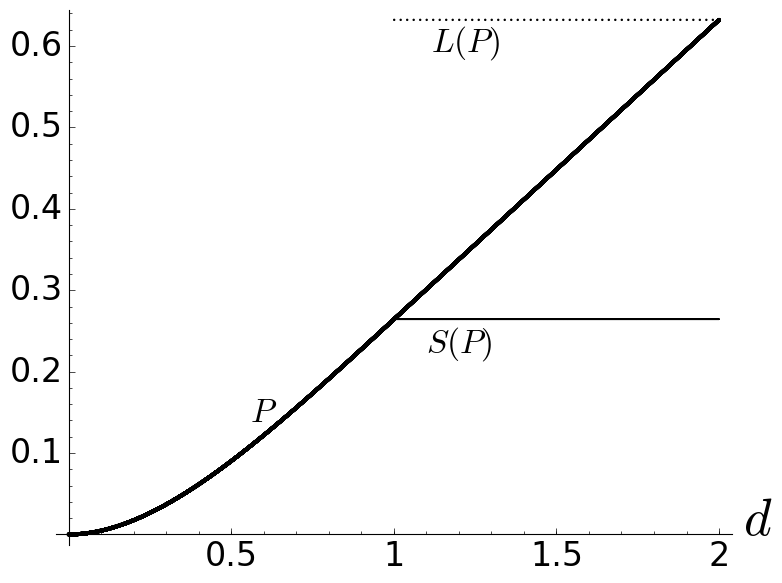
\includegraphics[scale=0.251]{cutvertices-planar.png}\hspace*{1cm}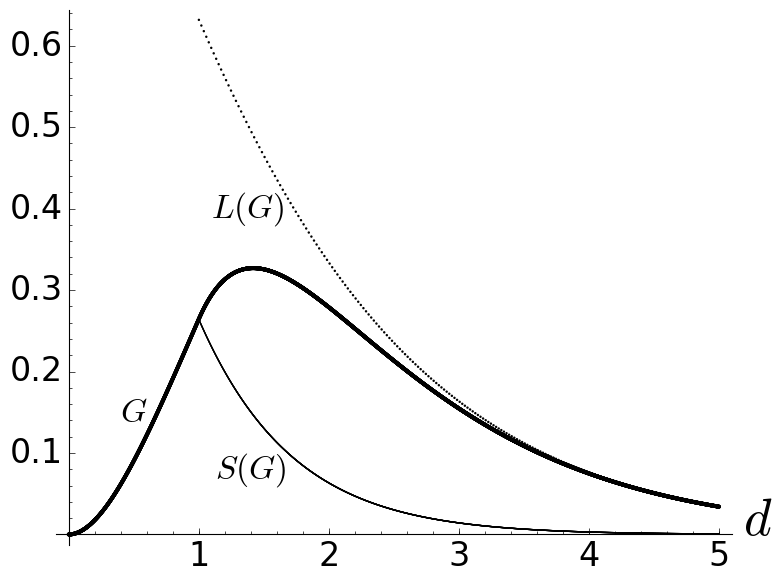
\includegraphics[scale=0.251]{cutvertices-ER.png}
\caption{Fraction of cut vertices in $P=P(n,m)$ and $G=G(n,m)$, where $m=m(n)$ is such that $2m/n\to d$.}
\label{fig:cv}
\end{figure}
\Cref{thm:planar_sub,thm:er_sub} show that $\cv{P}$ and $\cv{G}$ coincide asymptotically as long as $m\leq n/2+\bigo{n^{2/3}}$. However, \Cref{thm:planar_sup,thm:er_sup} reveal a completely different behaviour of $\cv{P}$ and $\cv{G}$ beyond this region (see also \Cref{fig:cv}). We could not find the results of \Cref{thm:er_sub,thm:er_sup} in literature and therefore, we provide sketches of their proofs in \Cref{sec:er}. In \Cref{sec:planar}, we show \Cref{thm:planar_sub,thm:planar_sup}. 
	
\section{Cut vertices in the \ER\ random graph}\label{sec:er}
To prove \Cref{thm:er_sub,thm:er_sup} on the number of cut vertices in the \ER\ random graph $G=G(n,m)$, we will use the following facts (see e.g. \cite{Bollobas2001}).
\begin{thm}\label{thm:er}
Let $k\in \N$, $G=G(n,m)$, $L=L(G)$ be the largest component of $G$, and $m=m(n)$ be such that $2m/n \to d\geq 0$. Then whp \textup{(i)} $v(L)=\left(\beta_d+\smallo{1}\right)n$, \textup{(ii)} the second largest component of $G$ has $\smallo{n}$ vertices, and \textup{(iii)} $\left|\left\{v\in V(G)\mid d_G(v)=k\right\}\right|=\left(e^{-d}d^k/k!+\smallo{1}\right) n$.
\end{thm}
{\itshape Sketch proofs of \Cref{thm:er_sub,thm:er_sup}.}~
We estimate the number $X^{(k)}$ of cut vertices in $G$ with $d_G(v)=k$ for $k\geq 2$. Let $X_v^{(k)}=1$ if $v\in V(G)$ is a cut vertex and $d_G(v)=k$, otherwise we set $X_v^{(k)}=0$. We construct $G$ conditioned on the event $d_G(v)=k$: We choose a random graph $G'$ on vertex set $[n]\setminus\{v\}$ with $m-k$ edges and then pick independently a set $N_v\subseteq [n]\setminus\{v\}$ for the $k$ neighbours of $v$. Now $v$ is not a cut vertex if and only if all $k$ vertices of $N_v$ lie in the same component of $G'$. As $G'$ is distributed like $G(n-1,m-k)$, \Cref{thm:er} implies that whp the largest component of $G'$ has $\left(\beta_d+\smallo{1}\right)n$ vertices, while all other components have $o(n)$ vertices. Together with \Cref{thm:er} this shows $\prob{X_v^{(k)}=1}=e^{-d}d^k/k! \cdot \left(1-\beta_d^k\right)+\smallo{1}$. Similarly, we obtain $\prob{X_v^{(k)}=X_w^{(k)}=1}=\left(e^{-d}d^k/k! \cdot \left(1-\beta_d^k\right)\right)^2+\smallo{1}$ for $v\neq w$. Hence, whp $X^{(k)}=\left(e^{-d}d^k(1-\beta_d^k)/k!+\smallo{1}\right)n$ by the first and second moment method. Due to \Cref{thm:er} there are $\smallo{n}$ vertices $v\in V(G)$ with $d_G(v)=\smallomega{1}$. Thus, whp $ \cv{G}=\left(\sum_{k\geq 2}X^{(k)}  + o(n)\right)/n=\sum_{k\geq 2}\left(e^{-d}d^k(1-\beta_d^k)/k!\right)+\smallo{1}=1-\left(d+e^{d\beta_d}-d\beta_d\right)e^{-d}+\smallo{1}$, which proves the statements on $\cv{G}$. Similarly, we show the assertions on $\cv{L}$ and $\cv{S}$. \qed

\section{Cut vertices in the random planar graph}\label{sec:planar}
\subsection[Average degree at most one]{Average degree at most one: Proof of \Cref{thm:planar_sub}}
\Cref{thm:planar_sub} is a direct consequence of the following well-known fact from \cite{Britikov1989}.
\begin{thm}[\hspace{1sp}\cite{Britikov1989}]\label{thm:non_complex}
Let $G=G(n,m)$ and $m=m(n)\leq n/2+\bigo{n^{2/3}}$. Then we have $\liminf_{n \to \infty}~ \prob{G \text{ has no components with at least two cycles}}>0$.	
\end{thm}
{\itshape Proof of \Cref{thm:planar_sub}.}~
Due to \Cref{thm:non_complex} we have  $\liminf_{n \to \infty}~ \prob{G \text{ is planar}}>0$. Therefore, each property that holds whp in $G(n,m)$ is also true whp in $P(n,m)$ as long as $m\leq n/2+\bigo{n^{2/3}}$. Hence, \Cref{thm:planar_sub} follows by \Cref{thm:er_sub}. \qed
	
\subsection{Graph decomposition and conditional random graphs}\label{sub:decomp}
To show \Cref{thm:planar_sup} we use the graph decomposition as in \cite{KangMosshammerSpruessel2020}. Given a graph $H$, the {\em complex part} $Q(H)$ of $H$ is the union of all components with at least two cycles. The remaining part $U(H):=H\setminus Q(H)$ is called the {\em non-complex part} and we define $n_U(H):=v(U(H))$ and $m_U(H):=e(U(H))$. The {\em core} $C(H)$ is the maximal subgraph of $Q(H)$ with minimum degree at least two. We note that $Q(H)$ arises from $C(H)$ by replacing each vertex by a rooted tree. The following results of Kang, Mo{\ss}hammer, and Spr\"{u}ssel \cite{KangMosshammerSpruessel2020} will be useful. 
	
\begin{thm}[\hspace{1sp}\cite{KangMosshammerSpruessel2020}]\label{thm:internal_structure}
Let $P=P(n,m)$, $Q=Q(P)$ the complex part of $P$, $C=C(P)$ the core, $L=L(P)$ the largest component, and $S=S(P)=P\setminus L$. Moreover, let $U=U(P)$ be the non-complex part of $P$, $n_U=v(U)$, and $m_U=e(U)$. Assume $m=m(n)$ is such that $n/2+\smallomega{n^{2/3}}\leq m \leq n+\smallo{n\left(\log n\right)^{-2/3}}$ and $2m/n \to d\in[1,2]$. Then whp \textup{(i)} $v(C)=\smallo{v(Q)}$, \textup{(ii)} $v(L)=\left(d-1+\smallo{1}\right)n$, \textup{(iii)} $n_U=\smallomega{1}$, \textup{(iv)} $m_U= n_U/2+\bigo{hn_U^{2/3}}$ for each function $h=h(n)=\smallomega{1}$, \textup{(v)} $\left|V(L)\triangle V(Q)\right|=\smallo{v(L)}$, and \textup{(vi)} $\left|V(S)\triangle V(U)\right|=\smallo{v(S)}$.
\end{thm}
\Cref{thm:internal_structure}(v) and (vi) imply that whp $\cv{L}=\cv{Q}+\smallo{1}$ and $\cv{S}=\cv{U}+\smallo{1}$. Furthermore, \Cref{thm:internal_structure}(ii) allows us to compute $\cv{P}$ once $\cv{L}$ and $\cv{S}$ are known. Thus, it suffices to determine $\cv{Q}$ and $\cv{U}$, which we will do in \Cref{sub:complex,sub:non_complex}, respectively. We will compute $\cv{Q}$ and $\cv{U}$ conditioned that $P$ satisfies some properties. Then we will use the following definition and lemma from \cite{KangMissethan2021} to deduce $\cv{Q}$ and $\cv{U}$.
	
\begin{definition}[{\hspace{1sp}\cite[Definition 3.1]{KangMissethan2021}}]\label{def:feasible} 
Given a class $\mathcal{A}$ of graphs let $\mathcal{A}(n)$ be the subclass containing those graphs with vertex set $[n]$.
Let $S$ be a set  and $\Phi:\mathcal{A}\to S$ a function. We say that a sequence $\mathbf{a}=(a_n)_{n\in \N}$ is {\em feasible} for $\left(\mathcal{A}, \Phi\right)$ if for each $n \in \N$  there is a graph $H \in \mathcal{A}(n)$ such that $\Phi(H)=a_n$. Furthermore, for each $n\in \N$ we write $\left(A\mid\mathbf{a}\right)(n)$ for a graph chosen uniformly at random from the set $\left\{H \in \mathcal{A}(n): \Phi(H)=a_n\right\}$. We will often omit the dependence on $n$ and write $A\mid\mathbf{a}$ instead of $\left(A\mid\mathbf{a}\right)(n)$.
\end{definition}
\begin{lem}[{\hspace{1sp}\cite[Lemma 3.2]{KangMissethan2021}}]\label{lem:conditional_random_graphs}
Let $\mathcal{A}$ be a class of graphs, $A=A(n)$ a graph chosen uniformly at random from $\mathcal{A}(n)$, $S$ a set, $\Phi:\mathcal{A}\to S$ a function, and $\mathcal{R}$ a graph property, i.e. $\mathcal{R}$ is a set of graphs. If for every sequence $\mathbf{a}=(a_n)_{n\in \N}$ that is feasible for $\left(\mathcal{A}, \Phi\right)$ whp $A\mid\mathbf{a}\in \mathcal{R}$, then we have whp $A \in \mathcal{R}$.
\end{lem}
	
\subsection{Cut vertices in the complex part}\label{sub:complex}
Using the concept of \lq conditional\rq\ random graphs (see \Cref{def:feasible} and \Cref{lem:conditional_random_graphs}) we will determine $\cv{Q(P)}$ in this section. For a given core $C$ and $q\in\N$ we denote by $Q(C,q)$ a graph chosen uniformly at random from the class of all complex parts which have $C$ as its core and vertex set $[q]$. We observe that $Q(C,q)$ is distributed like $Q(P)$ conditioned on the event $C(P)=C$ and $v(Q(P))=q$. Furthermore, $Q(C,q)$ can be constructed by choosing a random forest $F$ on vertex set $[q]$ with $v(C)$ many tree components such that the vertices from $C$ lie all in different tree components. Then we obtain $Q(C,q)$ by replacing each vertex $v$ in $C$ by the tree component of $F$ which is rooted at $v$. Therefore, we estimate first $\cv{F}$ in \Cref{lem:cut_vertices_forest} and then deduce $\cv{Q(C,q)}$ in \Cref{lem:cut_vertices_complex}. To that end, we denote by $F(n,t)$ a forest chosen uniformly at random from the class of all forests on vertex set $[n]$ having exactly $t$ trees as components such that the vertices $1, \ldots, t$ lie all in different tree components.
\begin{lem}\label{lem:cut_vertices_forest}
Let $t=t(n)=\smallo{n}$ and $F=F(n,t)$ be the random forest. Then we have whp $\cv{F}=1-e^{-1}+\smallo{1}$.
\end{lem}
\begin{proof}
A vertex $v\in[n]\setminus[t]$ is a cut vertex in $F$ if and only if $d_F(v)\neq 1$. We set $X_v=1$ if $d_F(v)= 1$ and $X_v=0$ otherwise. As $t=\smallo{n}$, it suffices to prove whp $\sum_{v\in[n]\setminus[t]}X_v=\left(e^{-1}+\smallo{1}\right)n$. Each realisation $H$ of $F$ with $d_H(v)=1$ can be constructed by first choosing a forest $H'$ on vertex set $[n]\setminus\left\{v\right\}$ with $t$ tree components such that the vertices in $[t]$ lie all in different tree components. Then we obtain $H$ by picking a vertex $v'\in [n]\setminus\left\{v\right\}$ and adding the edge $vv'$ in $H'$. This implies $\prob{X_v=1}=t(n-1)^{n-t-2}\cdot(n-1)/\left(tn^{n-t-1}\right)=e^{-1}+\smallo{1}$. Similarly, we obtain $\prob{X_v=X_w=1}=t(n-2)^{n-t-3}\cdot(n-2)^2/\left(tn^{n-t-1}\right)=e^{-2}+\smallo{1}$ for all $v\neq w$. The statement follows by the first and second moment method.
\end{proof}
	
\begin{lem}\label{lem:cut_vertices_complex}
For each $n\in\N$, let $C=C(n)$ be a core, $q=q(n)\in\N$, and $Q=Q(C,q)$ be the random complex part with core $C$ and vertex set $[q]$. If $v(C)=\smallo{q}$, then whp $\cv{Q}=1-e^{-1}+\smallo{1}$.
\end{lem}
\begin{proof}
W.l.o.g. we assume $V(C)=[v(C)]$. We construct $Q$ by picking a random forest $F=F(q,v(C))$ and replacing each vertex $v$ in $C$ by the tree component of $F$ which is rooted at $v$. A vertex $v\in [q]\setminus[v(C)]$ is a cut vertex in $Q$ if and only if it is a cut vertex in $F$. Together with the fact $v(C)=\smallo{q}$ it implies  whp $\cv{Q}=\cv{F}+\smallo{1}$. Hence, whp $\cv{Q}=1-e^{-1}+\smallo{1}$ by \Cref{lem:cut_vertices_forest}.
\end{proof}
	
Finally, we use \Cref{lem:conditional_random_graphs} to transfer the result on the fraction of cut vertices in $Q(C,q)$ from \Cref{lem:cut_vertices_complex} to the complex part $Q(P)$ of $P$.
\begin{lem}\label{lem:cv_complex}
Let $P=P(n,m)$ and $Q=Q(P)$ be the complex part of $P$. Assume $m=m(n)$ is such that $n/2+\smallomega{n^{2/3}}\leq m \leq n+\smallo{n\left(\log n\right)^{-2/3}}$ and $2m/n \to d\in[1,2]$. Then whp $\cv{Q}=1-e^{-1}+\smallo{1}$.
\end{lem}
\begin{proof}
To use \Cref{lem:conditional_random_graphs}, let $\mathcal{A}(n)$ be the class of planar graphs $H$ with vertex set $[n]$ and $m$ edges satisfying $v(C(H))=\smallo{v(Q(H))}$. By \Cref{thm:internal_structure}(i) we have whp $P\in\mathcal{A}:=\cup_{n\in\N}\mathcal{A}(n)$. Let $\Phi$ be such that $\Phi(H)=\left(C(H), v(Q(H))\right)$ for each $H\in\mathcal{A}$, $A=A(n)$ be a graph chosen uniformly at random from $\mathcal{A}(n)$, and $\mathbf{a}=(C_n, q_n)_{n\in\N}$ be a sequence that is feasible for $\left(\mathcal{A},\Phi\right)$. We note that $Q(A \mid \mathbf{a})$ is distributed like the random complex part $Q(C_n, q_n)$. Thus, we get by \Cref{lem:cut_vertices_complex} that whp $\cv{Q(A \mid \mathbf{a})}=1-e^{-1}+\smallo{1}$. Combining it with \Cref{lem:conditional_random_graphs} yields whp $\cv{Q(A)}=1-e^{-1}+\smallo{1}$. This shows the statement, since whp $P\in\mathcal{A}$.
\end{proof}
	
\subsection{Cut vertices in the non-complex part}\label{sub:non_complex}
 For given $n,m\in\N$ let $U(n,m)$ be a graph chosen uniformly at random from all graphs with vertex set $[n]$ and $m$ edges in which every component has at most one cycle. First we will determine $\cv{U(n,m)}$ and then deduce $\cv{U(P)}$.
\begin{lem}\label{lem:cv_non_complex}
Let $U=U(n,m)$ and $m=m(n)\leq n/2+\bigo{n^{2/3}}$ such that $2m/n \to d\in[0,1]$. Then whp $\cv{U}=1-(d+1)e^{-d}+\smallo{1}$.	
\end{lem}
\begin{proof}
The assertion follows by combining \Cref{thm:er_sub,thm:non_complex}. 
\end{proof}
\begin{lem}\label{lem:cv_non_complex1}
Let $P=P(n,m)$ and $U=U(P)$ be the non-complex part of $P$. Assume $m=m(n)$ is such that $n/2+\smallomega{n^{2/3}}\leq m \leq n+\smallo{n\left(\log n\right)^{-2/3}}$ and $2m/n \to d\in[1,2]$. Then whp $\cv{U}=1-2e^{-1}+\smallo{1}$.
\end{lem}
\begin{proof}
To use \Cref{lem:conditional_random_graphs}, let $\mathcal{A}(n)$ be the class of planar graphs $H$ with vertex set $[n]$ and $m$ edges satisfying $n_U(H)=\smallomega{1}$ and $m_U(H)=n_U(H)/2+\bigo{n_U(H)^{2/3}}$. By \Cref{thm:internal_structure}(iii) and (iv) we can choose the implicit constants in these equations such that $P\in\mathcal{A}:=\cup_{n\in\N}\mathcal{A}(n)$ with a probability of at least $1-\delta$, where $\delta>0$ is a given constant. Let $\Phi$ be such that $\Phi(H)=\left(n_U(H), m_U(H)\right)$ for each $H\in\mathcal{A}$, $A=A(n)$ be a graph chosen uniformly at random from $\mathcal{A}(n)$ and $\mathbf{a}=(\nu_n, \mu_n)_{n\in\N}$ be a sequence that is feasible for $\left(\mathcal{A},\Phi\right)$. By \Cref{lem:cv_non_complex} we get whp $\cv{U(A \mid \mathbf{a})}=1-2e^{-1}+\smallo{1}$, as $U(A \mid \mathbf{a})$ is distributed like $U(\nu_n, \mu_n)$. Together with \Cref{lem:conditional_random_graphs} this implies whp $\cv{U(A)}=1-2e^{-1}+\smallo{1}$. Using $\prob{P\in\mathcal{A}}>1-\delta$, we obtain that $\cv{U(P)}=1-2e^{-1}+\smallo{1}$ holds with a probability of at least $1-2\delta$. The statement follows, as $\delta>0$ was arbitrary.
\end{proof}
	
\subsection[Average degree between one and two]{Average degree between one and two: Proof of \Cref{thm:planar_sup}}
Let $Q=Q(P)$ be the complex part of $P$. By \Cref{thm:internal_structure}(v) we have whp $\cv{L}=\cv{Q}+\smallo{1}$ and \Cref{lem:cv_complex} states that whp $\cv{Q}=1-e^{-1}+\smallo{1}$. Thus, whp $\cv{L}=1-e^{-1}+\smallo{1}$. Due to \Cref{thm:internal_structure}(vi) and \Cref{lem:cv_non_complex1} we have whp $\cv{S}=\cv{U}+\smallo{1}=1-2e^{-1}+\smallo{1}$, where $U=U(P)$ is the non-complex part of $P$. Finally, by \Cref{thm:internal_structure}(ii) we have whp $v(L)=\left(d-1+\smallo{1}\right)n$. Thus, we get whp $\cv{P}=\left(\cv{L}v(L)+\cv{S}v(S)\right)/n=1-(3-d)e^{-1}+\smallo{1}$. \qed

% !TEX root = phd-missethan.tex

\def\seq{\mathbf{a}} %sequence
\def\property{\mathcal{R}}
\renewcommand{\Rest}{R}
\renewcommand{\rest}[1]{R\left(#1\right)} %graph without largest component ('rest')

\chapter{Maximum degree of random planar graphs}\label{cha:max_degree}

\section{Introduction and results}\label{MDsec:intro}

\subsection{Motivation}\label{MDsubsec:motivation}
The \ER\ random graph $G(n,m$), introduced by \Erdos\ and \Renyi\ \cite{ErdoesRenyi1959,ErdoesRenyi1960}, is a graph chosen uniformly at random from the class $\mathcal{G}(n,m)$ of all vertex-labelled graphs on vertex set $[n]:=\left\{1, \ldots, n\right\}$ with $m=m(n)$ edges, denoted by $G(n,m)\ur \mathcal{G}(n,m)$. Since its introduction $G(n,m)$, together with the closely related binomial random graph $G(n,p)$, has been intensively studied (see e.g. \cite{FriezeKaronski2016, JansonLuczakRucinski2000, Bollobas2001}). A remarkable feature of this model is the \lq concentration\rq\ of many graph parameters. That is, with high probability (meaning with probability tending to 1 as $n$ tends to infinity, {\em \whp\ } for short) certain graph parameters in $G(n,m)$ lie in \lq small\rq\ intervals, which only depend on $n$ and $m$.

The graph parameter we will focus on in this paper is the maximum degree of a graph $H$, denoted by $\maxdegree{H}$. \Erdos\ and \Renyi\ \cite{ErdoesRenyi1959} were the first to consider $\maxdegree{G(n,m)}$ and since then, many results on $\maxdegree{G(n,m)}$ and, more generally, the degree sequence of $G(n,m)$ were obtained (see e.g. \cite{Bollobas1980b,RiordanSelby2000,ErdosWilson1977,Bollobas1981,McKayWormald1997,Ivcenko1973,Bollobas1982}). A particular interesting result by \Bollobas\ \cite{Bollobas1982} is that $m\sim n\log n$ is a \lq threshold\rq\ for the concentration of $\maxdegree{G(n,m)}$. More formally, \whp\ $\maxdegree{G(n,m)}$ takes one of two values when $m=\smallo{n \log n}$, while $\maxdegree{G(n,m)}$ is not concentrated on any subset of $[n]$ with bounded size when $m=\smallomega{n \log n}$ and $m=\smallo{n^2}$.

\begin{thm}[{\hspace{1sp}\cite{Bollobas1982}}]\label{MDthm:max_degree_ergraph}
Let $m=m(n)=\smallo{n\log n}$ and $G=G(n,m)\ur \mathcal G(n,m)$. Then there exists a $\twoconcentration=\twoconcentration(n)\in \N$ such that \whp\ $\maxdegree{G}\in\left\{\twoconcentration, \twoconcentration+1\right\}$.
\end{thm}

\begin{thm}[{\hspace{1sp}\cite{Bollobas1982}}]\label{MDthm:max_degree_ergraph2}
	Let $m=m(n)=\smallomega{n\log n}$, $m=\smallo{n^2}$, and $G=G(n,m)\ur \mathcal G(n,m)$. If $I=I(n)\subseteq[n]$ is such that \whp\ $\maxdegree{G}\in I$, then $\left|I\right|=\smallomega{1}$.
\end{thm}

We note that \Bollobas\ \cite{Bollobas1982} actually considered the binomial random graph $G(n,p)$. But by using standard tools of relating $G(n,m)$ and $G(n,p)$ (see e.g. \cite[Section 1.1]{FriezeKaronski2016}) one can translate his results as stated in \Cref{MDthm:max_degree_ergraph,MDthm:max_degree_ergraph2}.

In recent decades various models of random graphs have been introduced by imposing additional constraints to $G(n,m)$, e.g. degree restrictions or topological constraints. In particular, random planar graphs and related structures, like random graphs on surfaces and random planar maps, have attained considerable attention \cite{ChapuyFusyGimenezMoharNoy2011,DowdenKangSpruessel2018,KangMosshammerSpruessel2020,McDiarmid2008,ChapuyFusyGimenezNoy2015,GimenezNoy2009,KangLuczak2012,McDiarmidStegerWelsh2005,McDiarmidReed2008,DrmotaGimenezNoyPanagiotouSteger2014,ColletDrmotaKlausner2019,DrmotaStufler2020,DrmotaNoyStufler2020,DrmotaGimenezNoy2011,Fusy2009,NoyRequileRue2020,PanagiotouSteger2011,FountoulakisPanagioutou2011,PanagiotouSteger2010,GerkeMcDiarmidStegerWeissl2005,GerkeMcDiarmid2004,GerkeSchlatterStegerTaraz2008,GerkeMcDiarmidStegerWeissl2007}. McDiarmid and Reed \cite{McDiarmidReed2008} considered the so-called $n$-vertex model for random planar graphs, that is, a graph $\planargraph(n)$ chosen uniformly at random from the class of all vertex-labelled planar graphs on vertex set $[n]$. They proved that \whp\ $\maxdegree{\planargraph(n)}=\Th{\log n}$. Later Drmota, Giménez, Noy, Panagiotou, and Steger \cite{DrmotaGimenezNoyPanagiotouSteger2014} used tools from analytic combinatorics and Boltzmann sampling techniques to show that \whp\ $\maxdegree{\planargraph(n)}$ is concentrated in an interval of length $\bigo{\log\log n}$. 

A more natural generalisation of $G(n,m)$ seems to be the random planar graph $\planargraph(n,m)$, which is a graph chosen uniformly at random from the class $\planarclass(n,m)$ of all vertex-labelled planar graphs on vertex set $[n]$ with $m=m(n)$ edges, denoted by $\planargraph(n,m)\ur \planarclass(n,m)$. The random planar graph $\planargraph(n,m)$ has been studied separately for the \lq sparse\rq\ regime where $m\leq n+\smallo{n}$ (see \cite{KangLuczak2012,KangMosshammerSpruessel2020}) and the \lq dense\rq\ regime where $m=\rounddown{\ratio n}$ for a constant $\ratio\in (1,3)$ (see e.g. \cite{GimenezNoy2009}). In this paper we show, in the flavour of \Cref{MDthm:max_degree_ergraph,MDthm:max_degree_ergraph2}, that in the sparse regime \whp\ $\maxdegree{\planargraph(n,m)}$ takes one of two values (see \Cref{MDthm:main,MDthm:main_sub}), while in the dense regime $\maxdegree{\planargraph(n,m)}$ is not concentrated on any subset of $[n]$ with bounded size (see \Cref{MDthm:main_dense}).

\subsection{Main results}\label{MDsubsec:main}
In order to state our main results, we need the following definition, where we denote by $\log$ the natural logarithm.
\begin{definition}\label{MDdef:nu}
	Let $\Concentration:\N^2\to \R^+$ be a function such that $\concentration{\nbins}{\nballs}$ is the unique positive zero of
	\begin{align*}
	f(x)=f_{\nbins, \nballs}(x)\defined x\log k+x-(x+1/2)\log x-(x-1)\log n.
	\end{align*}
	In case of $\nbins=\nballs$, we write $\specialconcentration{\nbins}:=\concentration{\nbins}{\nbins}$.
\end{definition}
In \Cref{MDsub:well_definedness} we will prove that the function $\Concentration$ is well defined, i.e. $f$ has a unique positive zero. In \Cref{MDlem:nu} we will provide some important properties of $\Concentration$ and in \Cref{MDsec:balls_bins} we motivate the definition of $\Concentration$ in the context of the balls-into-bins model.

We distinguish different cases according to which \lq region\rq\ the edge density falls into. The first regime which we consider is when $m\leq n/2+\bigo{n^{2/3}}$.

\begin{thm}\label{MDthm:main_sub}
Let $\planargraph=\planargraph(n,m)\ur \planarclass(n,m)$, $m=m(n)\leq n/2+\bigo{n^{2/3}}$, and $\varepsilon>0$. Then we have \whp\ $\rounddown{\concentration{n}{2m}-\varepsilon}\lessorequal \maxdegree{\planargraph}\lessorequal \rounddown{\concentration{n}{2m}+\varepsilon}$. In particular, \whp\ $\maxdegree{P}\in \left\{\twoconcentration, \twoconcentration+1\right\}$, where $\twoconcentration=\twoconcentration(n):=\rounddown{\concentration{n}{2m}-1/3}$.
\end{thm}

Next, we consider the case where $m\geq n/2+\smallomega{n^{2/3}}$ is such that $m\leq n+n^{1-\delta}$ for some $\delta>0$. Kang and \Luczak\ \cite{KangLuczak2012} and Kang, Moßhammer, and Sprüssel \cite{KangMosshammerSpruessel2020} showed that, in contrast to the case when $m\leq n/2+\bigo{n^{2/3}}$, in this regime \whp\ the largest component of $\planargraph=\planargraph(n,m)$ contains significantly more vertices than the second largest component. Therefore, we provide a concentration result on the maximum degree not only for $\planargraph$, but also for the largest component $\largestcomponent{\planargraph}$ of $\planargraph$ and the \lq rest\rq\ $\rest{\planargraph}:=\planargraph\setminus\largestcomponent{\planargraph}$. We will see that $\maxdegree{\largestcomponent{\planargraph}}$ and $\maxdegree{\rest{\planargraph}}$ are strongly concentrated around $\specialconcentration{\funcL}$ and $\specialconcentration{\funcR}$ for suitable $\funcL=\funcL(n)$ and $\funcR=\funcR(n)$, respectively. 

\begin{definition}\label{MDdef:functionLR}
Let $m=m(n)\geq n/2+\smallomega{n^{2/3}}$ be such that $m\leq n+n^{1-\delta}$ for some $\delta>0$. Then we define $\funcL=\funcL(n)$ and $\funcR=\funcR(n)$ as follows.	
\begin{center}
	\def\arraystretch{1.25}
	\begin{tabular}{l|c c }
	 \multicolumn{1}{c|}{ranges of $m$}	& $\funcL$ & $\funcR$
		\\
		\hline
		(a) $m=n/2+s$ for $s=s(n)>0$ such that $s=\smallo{n}$ and $s^3n^{-2}\to \infty$ & $s$ & $n$ \\
		(b) $m=d n/2$ where $d=d(n)$ tends to a constant in $\left(1,2\right)$ & $n$ & $n$ \\
		(c) $m=n+t$ for $t=t(n)<0$ such that $t=\smallo{n}$ and $t^5n^{-3}\to -\infty$ & $n$ & $\left|t\right|$ \\
		(d) $m=n+t$ for $t=t(n)$ such that $t^5n^{-3}$ tends to a constant in $\R$ & $n$ & $n^{3/5}$ \\
		(e) $m=n+t$ for $t=t(n)>0$ such that $t=\smallo{n}$ and $t^5n^{-3}\to \infty$ & $n$ & $n^{3/2}t^{-3/2}$\hspace{-0.05cm}
	\end{tabular}
\end{center}
\end{definition}

We note that $\funcL$ and $\funcR$ are chosen such that \whp\ the number of vertices in $\largestcomponent{\planargraph}$ and $\rest{\planargraph}$ are $\Th{\funcL}$ and $\Th{\funcR}$, respectively, according to results in \cite{KangMosshammerSpruessel2020,KangLuczak2012}. Throughout the paper, we will assume that if $m=m(n)\geq n/2+\smallomega{n^{2/3}}$ is such that $m\leq n+n^{1-\delta}$ for some $\delta>0$, then $m=m(n)$ lies in one of the five regimes considered in \Cref{MDdef:functionLR}, which is due to the critical phenomena observed in random planar graphs. Our next result states that in all these cases $\maxdegree{\planargraph}$, $\maxdegree{\largestcomponent{\planargraph}}$, and $\maxdegree{\rest{\planargraph}}$ are strongly concentrated. 

\begin{thm}\label{MDthm:main}
Let $\planargraph=\planargraph(n,m)\ur \planarclass(n,m)$, $\Largestcomponent=\largestcomponent{\planargraph}$ be the largest component of $\planargraph$, and $\Rest=\planargraph\setminus\Largestcomponent$. Assume $m=m(n)\geq n/2+\smallomega{n^{2/3}}$ is such that $m\leq n+n^{1-\delta}$ for some $\delta>0$. Let $\funcL=\funcL(n)$ and $\funcR=\funcR(n)$ be as in \Cref{MDdef:functionLR} and $\varepsilon>0$. Then \whp
\begin{enumerate}
	\item\label{MDthm:main1} $\rounddown{\specialconcentration{\funcL}-\varepsilon}+1\lessorequal \maxdegree{\Largestcomponent}\lessorequal \rounddown{\specialconcentration{\funcL}+\varepsilon}+1$;
	\item\label{MDthm:main2} $\rounddown{\specialconcentration{\funcR}-\varepsilon}\lessorequal \maxdegree{\Rest}\lessorequal \rounddown{\specialconcentration{\funcR}+\varepsilon}$.
\end{enumerate}
In particular, \whp\ we have that $\maxdegree{P}\in \left\{\twoconcentration, \twoconcentration+1\right\}$, where we let $\twoconcentration=\twoconcentration(n):=\max\left\{\rounddown{\specialconcentration{\funcL}+2/3}, \rounddown{\specialconcentration{\funcR}-1/3}\right\}$.
\end{thm}

For example, \Cref{MDthm:main} says that if $m=n/2+s$ for $s=s(n)>0$ such that $s=\smallo{n}$ and $s^3n^{-2}\to \infty$, known as the weakly supercritical regime, then \whp\ $\rounddown{\specialconcentration{s}-\varepsilon}+1\lessorequal \maxdegree{\Largestcomponent}\lessorequal \rounddown{\specialconcentration{s}+\varepsilon}+1$. In contrast, if $m=d n/2$ where $d=d(n)$ tends to a constant in $\left(1,2\right)$, which is the so-called intermediate regime, then \whp\ $\rounddown{\specialconcentration{n}-\varepsilon}+1\lessorequal \maxdegree{\Largestcomponent}\lessorequal \rounddown{\specialconcentration{n}+\varepsilon}+1$.

Combining \Cref{MDthm:main,MDthm:main_sub} we can determine the asymptotic order of $\maxdegree{\planargraph}$ in the sparse regime.
\begin{coro}\label{MDcor:maxdegree}
	Let $\planargraph=\planargraph(n,m)\ur \planarclass(n,m)$ and assume $m=m(n)$ is such that $\liminf_{n \to \infty} m/n>0$ and $m\leq n+n^{1-\delta}$ for some $\delta>0$. Then \whp
	\begin{align*}
	\maxdegree{\planargraph}=\left(1+\smallo{1}\right)\frac{\log n}{\log \log n}.
	\end{align*}
\end{coro}

It is well known that when $m\leq n/2+\bigo{n^{2/3}}$, the probability that $G(n,m)$ is planar is bounded away from 0 (see e.g. \Cref{MDthm:non_complex} and \cite{JansonKnuthLuczakPittel1993,LuczakPittelWierman1994,NoyRavelomananaRue2015}) and therefore, $\planargraph(n,m)$ \lq behaves\rq\ asymptotically like $G(n,m)$. However, this is not the case anymore when $m\geq n/2+\smallomega{n^{2/3}}$, since then \whp\ $G(n,m)$ is not planar (see \cite{LuczakPittelWierman1994,NoyRavelomananaRue2015}). \Cref{MDthm:main} reveals the following, perhaps surprising, difference between $\planargraph=\planargraph(n,m)$ and $G=G(n,m)$ in the case that $m=m(n)=d n/2$ where $d=d(n)$ tends to a constant in $\left(1,2\right)$. Roughly speaking, the maximum degrees $\maxdegree{\planargraph}$, $\maxdegree{\largestcomponent{\planargraph}}$, and $\maxdegree{\rest{\planargraph}}$ are {\em independent} of $d=d(n)$. Furthermore, $\maxdegree{\largestcomponent{\planargraph}}$ and $\maxdegree{\rest{\planargraph}}$ typically differ at most by two.

\begin{coro}\label{MDcor:independent}
Let $\planargraph=\planargraph(n,m)\ur \planarclass(n,m)$, $\Largestcomponent=\largestcomponent{\planargraph}$ be the largest component of $\planargraph$, and $\Rest=\planargraph\setminus\Largestcomponent$. There exists a $\twoconcentration=\twoconcentration(n)$ such that for all $m=m(n)=d n/2$ where $d=d(n)$ tends to a constant in $\left(1,2\right)$, we have \whp\ 
\begin{align*}
\maxdegree{\Largestcomponent}&\in \left\{\twoconcentration, \twoconcentration+1\right\};\\
\maxdegree{\Rest}&\in \left\{\twoconcentration-1, \twoconcentration\right\};\\
\maxdegree{\planargraph}&\in \left\{\twoconcentration, \twoconcentration+1\right\}.
\end{align*}
In particular, \whp\ $\maxdegree{\Rest}\leq\maxdegree{\Largestcomponent}\leq \maxdegree{\Rest}+2$.
\end{coro}

In contrast to \Cref{MDcor:independent}, $G=G(n,m)$ exhibits a perhaps more intuitive behaviour. If the average degree $d=2m/n$ is growing, then $\maxdegree{G}$ and $\maxdegree{\largestcomponent{G}}$ are increasing, while $\maxdegree{\rest{G}}$ is decreasing. As a consequence, $\maxdegree{\largestcomponent{G}}$ is typically much larger than $\maxdegree{\rest{G}}$. 

\begin{prop}\label{MDpro:ER}
For $i=1,2$, let $m_i=m_i(n)=d_i n/2$ where $d_i=d_i(n)$ tends to a constant $c_i>1$ and $G_i=G(n,m_i)\ur \mathcal G(n,m_i)$. If $c_1<c_2$ and $G_1$ and $G_2$ are chosen independently from each other, then \whp\ $\maxdegree{G_2}-\maxdegree{G_1}$, $\maxdegree{\largestcomponent{G_2}}-\maxdegree{\largestcomponent{G_1}}$, 	$\maxdegree{\rest{G_1}}-\maxdegree{\rest{G_2}}$, and $\maxdegree{\largestcomponent{G_1}}-\maxdegree{\rest{G_1}}$ are strictly positive and of order $\Th{\log n/\left(\log \log n\right)^2}$.
\end{prop}

We note that \Cref{MDpro:ER} follows by a generalised version of \Cref{MDthm:max_degree_ergraph} (see \Cref{MDthm:G_n_m_bins_balls}\ref{MDthm:G_n_m_bins_balls2}) and classical results on the \ER\ random graph $G(n,m)$. (For the sake of completeness, we provide a sketch of the proof of \Cref{MDpro:ER} in \Cref{MDsec:proof_er}.)

Finally, we consider the dense case when $m=m(n)=\rounddown{\ratio n}$ for $\ratio \in(1,3)$ and show that in this regime $\maxdegree{\planargraph}$ is not concentrated on any subset of $[n]$ with bounded size. 
\begin{thm}\label{MDthm:main_dense}
	Let $\planargraph=\planargraph(n,m)\ur \planarclass(n,m)$ and assume $m=m(n)=\rounddown{\ratio n}$ for $\ratio \in(1,3)$. If $I=I(n)\subseteq[n]$ is such that \whp\ $\maxdegree{\planargraph}\in I$, then $\left|I\right|=\smallomega{1}$.
\end{thm}

We note that in a planar graph on $n\geq 3$ vertices there are at most $3n-6$ edges, while a general (not necessarily planar) graph can have up to $\binom{n}{2}$ edges. In view of this fact, it seems natural that the \lq transition\rq\ from the two-point concentration to the non-concentration of the maximum degree occurs {\em much earlier} in $\planargraph(n,m)$ than in $G(n,m)$, namely at $m\sim n$ in $\planargraph(n,m)$ (cf. \Cref{MDthm:main_sub,MDthm:main,MDthm:main_dense}) instead of $m\sim n\log n$ in $G(n,m)$ (cf. \Cref{MDthm:max_degree_ergraph,MDthm:max_degree_ergraph2}). It is worth noting that the \lq threshold\rq\ where the number of vertices outside the largest component drops from linear to sublinear is $m\sim n$ for the random planar graph $\planargraph(n,m)$, while it is $m \sim n\log n$ in the case of $G(n,m)$.

\subsection{Outline of the paper} 
The rest of the paper is structured as follows. After giving the necessary definitions, notations, and concepts in \Cref{MDsec:prelim}, we provide our proof strategy in \Cref{MDsec:strategy}. \Cref{MDsec:balls_bins} is devoted to the balls-into-bins model, which we use in \Cref{MDsec:ergraph,MDsec:forests} to show concentration of the maximum degree in the \ER\ random graph, in a random graph without complex components, and in a random forest with specified roots, respectively. In \Cref{MDsec:proof,MDsec:planar_dense} we provide the proofs of our main results. Subsequently in \Cref{MDsec:nu}, we consider the function $\concentration{\nbins}{\nballs}$ introduced in \Cref{MDdef:nu} in more detail. In \Cref{MDsec:proof_pruefer,MDsec:proof_er} we proof results on $\maxdegree{G(n,m)}$ and a generalised version of Prüfer sequences, respectively. Finally in \Cref{MDsec:discussion}, we discuss a possible generalisation of our results and various questions that remain unanswered.

\section{Preliminaries}\label{MDsec:prelim}
\subsection{Notations for graphs}
We consider only undirected graphs or multigraphs and we always assume that the graphs are vertex-labelled.
\begin{definition}
	Given a (simple or multi) graph $H$ we denote by
	\begin{itemize}
		\item 
		$\vertexSet{H}$ the vertex set of $H$ and
		\item[]
		$\numberVertices{H}$ the order of $H$, i.e. the number of vertices in $H$;
		\item 
		$\edgeSet{H}$ the edge set of $H$ and
		\item[]
		$\numberEdges{H}$ the size of $H$, i.e. the number of edges in $H$;	
		\item 
		$\largestcomponent{H}$ the largest component of $H$;
		\item
		$\rest{H}:=H \setminus \largestcomponent{H}$ the graph obtained from $H$ by deleting the largest component;
		\item
		$\degree{v}{H}$ the degree of a vertex $v\in\vertexSet{H}$. Moreover, if $\vertexSet{H}=[n]$, then we call $\left(\degree{1}{H}, \ldots, \degree{n}{H}\right)$ the degree sequence of $H$.
	\end{itemize}
\end{definition}
\begin{definition}\label{MDdef:graph_class}
	Given a class $\cl$ of graphs (e.g. the class of planar graphs), we denote by 
	$\cl(n)$ the subclass of $\cl$ containing the graphs on vertex set $[n]$ 
	and by $\cl(n,m)$ the subclass of $\cl$ containing the graphs on vertex set $[n]$ with $m$ edges, respectively. We write $\randomGraph(n)\ur \cl(n)$ for a graph chosen uniformly at random from $\cl(n)$
	and $\randomGraph(n,m)\ur \cl(n,m)$ for a graph chosen uniformly at random from $\cl(n,m)$, respectively.
\end{definition}

\subsection{Random variables and asymptotic notation}
\begin{definition}
	Let $S$ be a finite set and let $Y$ and $Z$ be random variables with values in $S$. Then we say that $Y$ is {\em distributed like} $Z$, denoted by $Y\sim Z$, if for all $x \in S$ we have $\prob{Y=x}=\prob{Z=x}$.
\end{definition}
Throughout this paper, we use the standard Landau notation and all asymptotics are taken with respect to $n$, i.e. when $n\to \infty$. In order to express that two random variables have asymptotically a \lq similar\rq\ distribution, we use the notion of contiguity.
\begin{definition}
	For each $n\in\N$, let $S=S(n)$ be a finite set and let $Y=Y(n)$ and $Z=Z(n)$ be random variables with values in $S$. We say that $Z$ is {\em contiguous} with respect to $Y$, denoted by $\contiguous{Z}{Y}$, if for all sequences $I=I(n)\subseteq S(n)$
	\begin{align*}
		\left(\lim\limits_{n\to \infty}\prob{Y\in I}=1\right) ~\implies~ \left(\lim\limits_{n\to \infty}\prob{Z\in I}=1\right).
	\end{align*}
\end{definition}

\subsection{Complex part and core}\label{MDsub:decomposition}
We say that a component of a graph $H$ is {\em complex} if it has at least two cycles. The union of all complex components is called the {\em complex part} $\complexpart{H}$. We call the graph $H$ {\em complex} if all its components are complex. The union of all non-complex components is the {\em non-complex part} $\restcomplex{H}:=H\setminus \complexpart{H}$. The {\em core} $\core{H}$, also known as the 2-core, is the maximal subgraph of $\complexpart{H}$ of minimum degree at least two. We observe that the core $\core{H}$ can be obtained from $H$ by first removing vertices of degree one recursively and then deleting isolated cycles. We denote by $\complexlargestcore{H}$ the component of $\complexpart{H}$ containing the largest component of the core $\largestcomponent{\core{H}}$. The rest of the complex part is denoted by $\complexrestcore{H}:=\complexpart{H}\setminus\complexlargestcore{H}$. We call $\complexlargestcore{H}$ and $\complexrestcore{H}$ the {\em large complex part} and the {\em small complex part}, respectively. We note that the number of vertices in $\complexlargestcore{H}$ is not necessarily larger than in $\complexrestcore{H}$, but it will be true in most cases we consider. Using this decomposition we can split $H$ into the three disjoint parts $\complexlargestcore{H}$, $\complexrestcore{H}$, and $\restcomplex{H}$. Moreover, we have the relations $\core{\complexlargestcore{H}}=\largestcomponent{\core{H}}$ and $\core{\complexrestcore{H}}=\rest{\core{H}}$.

Later we will construct the large complex part, the small complex part, and the non-complex part of a random planar graph independently of each other. To that end, we will use the following two graph classes.
\begin{definition}\label{MDdef:random_complex_part}
	Let $C$ be a core, i.e. a graph with minimum degree at least two containing no isolated cycles, and $q\in \N$. Then we denote by $\complexclass(C,q)$ the class consisting of {\em complex} graphs having core $C$ and vertex set $[q]$. We let $\complexgraph(C,q)\ur\complexclass(C,q)$ be a graph chosen uniformly at random from this class.
\end{definition}

\begin{definition}\label{MDdef:nocomplex}
We denote by $\nocomplexclass$ the class consisting of all graphs without complex components. For $n,m\in\N$ we let $\nocomplexclass(n,m)\subseteq\nocomplexclass$ be the subclass of all graphs on vertex set $[n]$ with $m$ edges and we write $\nocomplex(n,m)\ur \nocomplexclass(n,m)$ for a graph chosen uniformly at random from $\nocomplexclass(n,m)$.
\end{definition}

\begin{remark}\label{MDrem:connection_conditional}
Let $C$ be a core, $q, n, m \in\N$, and $H\in\complexclass(C,q)$ be a fixed graph. Then there are precisely $\left|\nocomplexclass(u,w)\right|$ many graphs $H'\in\planarclass(n,m)$ whose complex part is $H$, where $u:=n-q$ and $w:=m-\numberEdges{C}+\numberVertices{C}-q$. As this number is independent of $H\in\complexclass(C,q)$, there is a nice relation between the complex part $\complexpart{\planargraph}$ of the random planar graph $\planargraph=\planargraph(n,m)$ and $\complexgraph(C,q)\ur\complexclass(C,q)$, the latter being as in \Cref{MDdef:random_complex_part}: Conditioned on the event that the core $\core{\planargraph}$ is $C$ and $\numberVertices{\complexpart{\planargraph}}=q$, the complex part $\complexpart{\planargraph}$ is distributed like $\complexgraph(C,q)$. Similarly, for fixed $\tilde{n},\tilde{m},n,m \in \N$ let $\restcomplex{\planargraph}$ be the non-complex part of $\planargraph$ and $\nocomplex(\tilde{n},\tilde{m})\ur \nocomplexclass(\tilde{n},\tilde{m})$ be as in \Cref{MDdef:nocomplex}. Then, conditioned on the event that $\numberVertices{\restcomplex{\planargraph}}=\tilde{n}$ and $\numberEdges{\restcomplex{\planargraph}}=\tilde{m}$, the non-complex part $\restcomplex{\planargraph}$ is distributed like $\nocomplex(\tilde{n},\tilde{m})$.
\end{remark}

\subsection{Conditional random graphs}\label{MDsub:conditional_random_graphs}
Given a class $\cl$ of graphs it is sometimes quite difficult to directly analyse the random graph $\randomGraph=\randomGraph(n)\ur\cl(n)$. In such cases we will use the idea of conditional random graphs. Loosely speaking, we split $\cl$ into disjoint subclasses and consider for each subclass $\tilde{\cl}$ the random graph $\tilde{\randomGraph}=\tilde{\randomGraph}(n)\ur \tilde{\cl}(n)$, in other words, the random graph $\randomGraph$ conditioned on the event that $\randomGraph\in \tilde{\cl}$. If we can show that some graph property holds in all these \lq conditional\rq\ random graphs \whp, then \whp\ this property holds also in $\randomGraph$. The following definition and lemma make that idea more precise.
\begin{definition}\label{MDdef:feasible}
	Given a class $\cl$ of graphs, a set $S$, and a function $\func:\cl\to S$, we call a sequence $\seq=(\term_n)_{n\in \N}$ {\em feasible} for $\left(\cl, \func\right)$ if for each $n \in \N$ there exists a graph $H \in \cl(n)$ such that $\func(H)=\term_n$. Moreover, for each $n\in \N$ we denote by $\left(\condGraph{\randomGraph}{\seq}\right)(n)$ a graph chosen uniformly at random from the set $\left\{H \in \cl(n): \func(H)=\term_n\right\}$. We will often omit the dependence on $n$ and write just $\condGraph{\randomGraph}{\seq}$ (i.e. \lq $\randomGraph$ conditioned on $\seq$\rq) instead of $\left(\condGraph{\randomGraph}{\seq}\right)(n)$.
\end{definition}
\begin{lem}[\hspace{1sp}{\cite[Lemma 3.2]{KangMissethan2021}}]\label{MDlem:conditional_random_graphs}
	Let $\cl$ be a class of graphs, $S$ a set, $\func:\cl\to S$ a function, $\property$ a graph property, and $\randomGraph=\randomGraph(n)\ur \cl(n)$. If for every sequence $\seq=(\term_n)_{n\in \N}$ that is feasible for $\left(\cl, \func\right)$ we have \whp\ $\condGraph{\randomGraph}{\seq} \in \property$, then we have \whp\ $\randomGraph \in \property$.
\end{lem}

\subsection{Internal structure of a random planar graph}\label{MDsub:internal_structure}
In the proofs of our main results we will use some results from \cite{KangLuczak2012,KangMosshammerSpruessel2020} on the internal structure of a random planar graph $\planargraph(n,m)$, e.g. asymptotic order of the core, which are reformulated to simplify asymptotic notation. 
\begin{thm}[{\hspace{1sp}\cite{KangLuczak2012,KangMosshammerSpruessel2020}}]\label{MDthm:internal_structure}
	Let $\planargraph=\planargraph(n,m)\ur \planarclass(n,m)$, $C=\core{\planargraph}$ be the core, $\Complexlargestcore=\complexlargestcore{\planargraph}$ the large complex part, $\Complexrestcore=\complexrestcore{\planargraph}$ the small complex part, $\Restcomplex=\restcomplex{\planargraph}$ the non-complex part, and $\Largestcomponent=\largestcomponent{\planargraph}$ the largest component of $\planargraph$. In addition, let $h=h(n)=\smallomega{1}$ be a function tending to $\infty$ arbitrarily slowly and $\funcL=\funcL(n)$ and $\funcR=\funcR(n)$ be as in \Cref{MDdef:functionLR}. We assume that $m=m(n)\geq n/2+\smallomega{n^{2/3}}$ is such that $m\leq n+n^{1-\delta}$ for some $\delta>0$ and let $\beta:=\min\left\{\delta/2,1/5\right\}$. Then \whp\ the following hold.
\begin{enumerate}
\item\label{MDthm:internal_structure1}
$\maxdegree{C}=\Th{1}$;
\item\label{MDthm:internal_structure2}
$\numberVertices{\largestcomponent{C}}=\bigo{\funcL^{1-\beta}}$;
\item\label{MDthm:internal_structure3}
$\Complexlargestcore=\Largestcomponent$;
\item\label{MDthm:internal_structure4}
$\numberVertices{\Complexlargestcore}=\Th{\funcL}$;
\item\label{MDthm:internal_structure5}
$\numberVertices{\Complexrestcore}=\bigo{h\funcR^{2/3}}$;
\item\label{MDthm:internal_structure6}
$\numberVertices{\Restcomplex}=\Th{\funcR}$;
\item\label{MDthm:internal_structure7}
$\numberEdges{\Restcomplex}=\numberVertices{\Restcomplex}/2+\bigo{h\numberVertices{\Restcomplex}^{2/3}}$.
\end{enumerate}	
\end{thm}

\subsection[Properties of \lq concentration-function\rq]{Properties of \texorpdfstring{$\concentration{\nbins}{\nballs}$}{nu(n,k)}}
We will use the following basic properties of $\concentration{\nbins}{\nballs}$ introduced in \Cref{MDdef:nu}. 
\begin{lem}\label{MDlem:nu}
Let the function $\concentration{\nbins}{\nballs}$ be defined as in \Cref{MDdef:nu} and $\specialconcentration{\nbins}=\concentration{n}{n}$. Then we have
\begin{enumerate}
\item \label{MDlem:nu5} $\concentration{\nbins}{\nballs}>1$ for all $\nbins, \nballs \in \N$;
\item \label{MDlem:nu7} if $\nballs=\nballs(\nbins)=\bigo{n^{1/3}}$, then $\concentration{\nbins}{\nballs}\leq 5/3+\smallo{1}$;
\item \label{MDlem:nu1} if $\nballs=\nballs(\nbins)=\Th{\nbins}$, then $\concentration{\nbins}{\nballs}=\left(1+\smallo{1}\right)\log \nbins/\log\log\nbins$;
\item \label{MDlem:nu8} if $\nballs=\nballs(\nbins)=\bigo{\nbins}$, then $\concentration{\nbins}{\nballs}=\smallo{\log n}$;
\item \label{MDlem:nu6}
if $\nballs=\nballs(\nbins)=\bigo{\nbins}$, then $\concentration{\nbins}{\nballs}=\smallomega{\nballs/\nbins}$;
\item \label{MDlem:nu4} $\concentration{\nbins}{\nballs}$ is strictly increasing in the argument $\nballs$;
\item \label{MDlem:nu3} if $\nballs=\nballs(\nbins)=\Th{\nbins}$ and $d=d(n)=\smallo{\nbins\left(\log \log \nbins\right)^2/\log \nbins}$, then $\concentration{\nbins}{\nballs+d}-\concentration{\nbins}{\nballs}=\smallo{1}$;
\item \label{MDlem:nu9} $\specialconcentration{\nbins}$ is strictly increasing;
\item \label{MDlem:nu2} if $c=c(\nbins)=\Th{1}$ and $\nballs=\nballs(\nbins)=\Th{\nbins}$, then $\concentration{c\nbins}{c\nballs}=\concentration{\nbins}{\nballs}+\smallo{1}$;
\item \label{MDlem:nu10} if $c=c(\nbins)=\Th{1}$, then $\concentration{\nbins}{c\nbins}-\specialconcentration{\nbins}=\left(\log c+\smallo{1}\right)\log n/\left(\log \log n\right)^2$.
\end{enumerate}
\end{lem}
We provide a proof of \Cref{MDlem:nu} in \Cref{MDsub:proof_nu}.

\section{Proof strategy}\label{MDsec:strategy}
In order to prove \Cref{MDthm:main_sub} on the two-point concentration of $\maxdegree{\planargraph(n,m)}$ when $m\leq n/2+\bigo{n^{2/3}}$, we will use the known fact that with positive probability the \ER\ random graph $G(n,m)$ is planar in this regime (see \Cref{MDthm:non_complex}). Thus, it suffices to determine $\maxdegree{G(n,m)}$ instead of $\maxdegree{P(n,m)}$, which we will do by proving that $\maxdegree{G(n,m)}$ \lq behaves\rq\ like the maximum load of an appropriate ball-into-bins model (see \Cref{MDsub:strategy_without_complex} for details).

The proof of \Cref{MDthm:main} will be based on the following result on the typical structure of $\planargraph=\planargraph(n,m)$, which can be derived by using statements from \cite{KangLuczak2012,KangMosshammerSpruessel2020}: Informally speaking, the largest component $\Largestcomponent=\largestcomponent{\planargraph}$ consists of a family $F$ of rooted tree components, which are connected via \lq few\rq\ edges between the {\em roots} of the tree components that are exactly the vertices of $\largestcomponent{\core{\planargraph}}$, i.e. the largest component of the core. The number of tree components in $F$ is much smaller than $\numberVertices{F}$, because the order of the core is typically much smaller than the order of the largest component (see \Cref{MDthm:internal_structure}\ref{MDthm:internal_structure2} and \ref{MDthm:internal_structure4}). In addition, the remaining part $\Rest=\rest{\planargraph}=\planargraph\setminus\Largestcomponent$ \lq behaves\rq\ like an \ER\ random graph $G(\tilde{n}, \tilde{n}/2)$ for a suitable $\tilde{n}=\tilde{n}(n)$. We refer to \Cref{MDfig:typical_structure} for an illustration of this structure. 

Then we will derive the two-point concentration of $\maxdegree{\Rest}$ by studying $G(\tilde{n}, \tilde{n}/2)$. Using the property that the number of tree components in $F$, and therefore also the number of roots, is small compared to $\numberVertices{F}$, we will show that the degrees of the roots are typically much smaller than $\maxdegree{F}$ (see \Cref{MDthm:forest_max_degree}\ref{MDthm:forest_max_degree2}). Together with the fact that the number of \lq additional\rq\ edges connecting the roots is \lq small\rq, this will yield $\maxdegree{L}=\maxdegree{F}$. Then the two-point concentration of $\maxdegree{L}$ will follow by analysing $\maxdegree{F}$ via the balls-into-bins model and Prüfer sequences (see \Cref{MDsec:forests}). In the following sections we will describe these ideas in more detail. In \Cref{MDsub:strategy_decomposition} we will use a graph decomposition and conditional random graphs to make the aforementioned structural result on $\planargraph$ more formal. Subsequently, we determine the maximum degrees of $F$ and $G(n,m)$ in \Cref{MDsub:strategy_complex_part,MDsub:strategy_without_complex}, respectively. 

\begin{figure}[t]
		\begin{tikzpicture}[scale=0.72, line width=0.65mm, every node/.style={circle,fill=gray,draw,line width=0.25mm,inner sep=0,minimum size=0.21cm}]

	\node (A) at (0,0) [draw,rectangle] {};
	\node (B) at (0.5,-0.95) [draw,rectangle] {};
	\node (C) at (1.5,-1.4) [draw,rectangle] {};
	\node (D) at (2.5,-0.95) [draw,rectangle] {};
	\node (E) at (3,0) [draw,rectangle] {};
	\node (F) at (2.5,0.95) [draw,rectangle] {};
	\node (G) at (1.5,1.4) [draw,rectangle] {};
	\node (H) at (0.5,0.95) [draw,rectangle] {};
	
	\node (I) at (4.2,0) [draw,rectangle] {};
	\node (J) at (5,1) [draw,rectangle] {};
	\node (K) at (6.2,0.7) [draw,rectangle] {};
	\node (L) at (6.2,-0.7) [draw,rectangle] {};
	\node (M) at (5,-1) [draw,rectangle] {};
		
	\node (N) at (5.8,-1.7) [draw] {};
	\node (O) at (5,-1.9) [draw] {};
	\node (P) at (6.6,-1.3) [draw] {};
	\node (Q) at (7.4,-1.1) [draw] {};
	\node (R) at (6.5,-2.3) [draw] {};
	\node (S) at (8.1,-0.7) [draw] {};
	\node (T) at (8.8,-0.4) [draw] {};
	\node (U) at (7.1,-1.8) [draw] {};
	\node (V) at (7.8,-1.8) [draw] {};
	\node (W) at (5.5,-2.7) [draw] {};
	\node (X) at (7.4,-2.5) [draw] {};
	\node (Y) at (8.5,-1.6) [draw] {};
	\node (Z) at (8.3,-2.3) [draw] {};
	\draw[-] (M) to (N);
	\draw[-] (M) to (O);
	\draw[-] (N) to (P);
	\draw[-] (P) to (Q);
	\draw[-] (N) to (R);
	\draw[-] (Q) to (S);
	\draw[-] (S) to (T);
	\draw[-] (P) to (U);
	\draw[-] (U) to (V);
	\draw[-] (U) to (X);
	\draw[-] (O) to (W);
	\draw[-] (V) to (Y);
	\draw[-] (V) to (Z);
	
	\node (1) at (2.7,-1.9) [draw] {};
	\node (2) at (3.3,-1.3) [draw] {};
	\node (3) at (3.3,-2.1) [draw] {};
	\node (4) at (4,-1.3) [draw] {};
	\node (5) at (3.9,-1.8) [draw] {};
	\node (6) at (4.5,-2.3) [draw] {};
	\draw[-] (D) to (1);
	\draw[-] (D) to (2);
	\draw[-] (2) to (3);
	\draw[-] (2) to (4);
	\draw[-] (2) to (5);
	\draw[-] (5) to (6);
	
	\node (7) at (7,1.1) [draw] {};
	\node (8) at (7,0.35) [draw] {};
	\node (9) at (7.7,1.1) [draw] {};
	\draw[-] (K) to (7);
	\draw[-] (K) to (8);
	\draw[-] (7) to (9);
	
	\node (10) at (0.6,-1.5) [draw] {};
	\node (11) at (-0.3,-1.5) [draw] {};
	\node (12) at (-1,-1.1) [draw] {};
	\node (13) at (-1,-1.8) [draw] {};
	\node (14) at (-1.7,-2) [draw] {};
	\node (15) at (-1.7,-1.5) [draw] {};
	\node (16) at (-1.7,-0.7) [draw] {};
	\node (17) at (-1.7,-1.1) [draw] {};
	\node (18) at (-2.2,-0.5) [draw] {};
	\node (19) at (-2.2,-1.1) [draw] {};
	
	\draw[-] (C) to (10);
	\draw[-] (10) to (11);
	\draw[-] (11) to (12);
	\draw[-] (11) to (13);
	\draw[-] (13) to (14);
	\draw[-] (12) to (15);
	\draw[-] (12) to (16);
	\draw[-] (12) to (17);
	\draw[-] (16) to (18);
	\draw[-] (17) to (19);
	
	\node (20) at (4.4,1.2) [draw] {};
	\node (21) at (5.6,1.2) [draw] {};
	\draw[-] (J) to (20);
	\draw[-] (J) to (21);
	
	\node (22) at (-0.7,0.3) [draw] {};
	\node (23) at (-1.3,0.5) [draw] {};
	\draw[-] (A) to (22);
	\draw[-] (22) to (23);
	
	\node (24) at (3.2,1.2) [draw] {};
	\draw[-] (F) to (24);
		
	\draw[-,thin] (A) to (B);
	\draw[-,thin] (B) to (C);
	\draw[-,thin] (C) to (D);
	\draw[-,thin] (D) to (E);
	\draw[-,thin] (E) to (F);
	\draw[-,thin] (F) to (G);
	\draw[-,thin] (G) to (H);
	\draw[-,thin] (H) to (A);
	\draw[-,thin] (C) to (H);
	\draw[-,thin] (I) to (J);
	\draw[-,thin] (J) to (K);
	\draw[-,thin] (K) to (L);
	\draw[-,thin] (L) to (M);
	\draw[-,thin] (M) to (I);
	\draw[-,thin] (E) to (I);
	
	\draw[-, thin] (-2.5,-3) to (-2.5,-3.1);
	\draw[-, thin] (-2.5,-3.1) to (9,-3.1);
	\draw[-, thin] (9,-3) to (9,-3.1);
	\node () at (3.75,-3.5) [draw=none, rectangle, fill=white] {$L$};
	
	\node (25) at (11.5,1.4) [draw] {};
	\node (26) at (11.5,0.8) [draw] {};
	\node (27) at (11.5,0.2) [draw] {};
	\node (28) at (11.8,-0.4) [draw] {};
	\node (29) at (11.1,-0.4) [draw] {};
	\node (30) at (11.1,-1) [draw] {};
	\node (31) at (10.8,-1.6) [draw] {};
	\node (32) at (11.4,-1.6) [draw] {};
	
	\draw[-] (25) to (26);
	\draw[-] (26) to (27);
	\draw[-] (27) to (28);
	\draw[-] (27) to (29);
	\draw[-] (29) to (30);
	\draw[-] (30) to (31);
	\draw[-] (30) to (32);
	
	\node (33) at (13,1.4) [draw] {};
	\node (34) at (12.6,0.8) [draw] {};
	\node (35) at (13.4,0.8) [draw] {};
	\node (36) at (13.1,0.2) [draw] {};
	\node (37) at (13.7,0.2) [draw] {};
	\node (38) at (13.1,-0.4) [draw] {};
	\draw[-] (33) to (34);
	\draw[-] (33) to (35);
	\draw[-] (35) to (36);
	\draw[-] (35) to (37);
	\draw[-] (36) to (38);
	
	\node (39) at (12.5,-1.2) [draw] {};
	\node (40) at (13.1,-1.2) [draw] {};
	\node (41) at (13.7,-0.8) [draw] {};
	\node (42) at (13.7,-1.6) [draw] {};
	\draw[-] (39) to (40);
	\draw[-] (40) to (41);
	\draw[-] (40) to (42);
	
	\node (43) at (14.4,1.3) [draw] {};
	\node (44) at (15.1,1.3) [draw] {};
	\draw[-] (43) to (44);
	
	\node (45) at (14.4,0.6) [draw] {};
	\node (46) at (15.1,0.6) [draw] {};
	\draw[-] (45) to (46);
	
	\node (47) at (14.4,-0.1) [draw] {};
	\node (48) at (15.1,-0.1) [draw] {};
	\draw[-] (47) to (48);
	
	\node (49) at (14.4,-0.8) [draw] {};
	\node (50) at (15.1,-0.8) [draw] {};
	\draw[-] (49) to (50);
	
	\node (51) at (14.4,-1.5) [draw] {};
	\node (52) at (15.1,-1.5) [draw] {};
	\draw[-] (51) to (52);
	
	\node (53) at (16.1,1.4) [draw] {};
	\node (54) at (16.9,1.4) [draw] {};
	\node (55) at (16.1,0.8) [draw] {};
	\node (56) at (16.9,0.8) [draw] {};
	\node (57) at (16.1,0.2) [draw] {};
	\node (58) at (16.9,0.2) [draw] {};
	\node (59) at (16.1,-0.4) [draw] {};
	\node (60) at (16.9,-0.4) [draw] {};
	\node (61) at (16.1,-1) [draw] {};
	\node (62) at (16.9,-1) [draw] {};
	\node (63) at (16.1,-1.6) [draw] {};
	\node (64) at (16.9,-1.6) [draw] {};
	
	\draw[-, thin] (10.5,-2.1) to (10.5,-2.2);
	\draw[-, thin] (10.5,-2.2) to (17.2,-2.2);
	\draw[-, thin] (17.2,-2.1) to (17.2,-2.2);
	\node () at (13.75,-2.7) [draw=none, fill=white, rectangle] {$R$};	
\end{tikzpicture}
\caption{Typical structure of $\planargraph=\planargraph(n,m)$ when $m$ is as in \Cref{MDthm:main}: The largest component $\Largestcomponent=\largestcomponent{\planargraph}$ consists of a family of rooted tree components, which are connected via \lq few\rq\ edges (drawn with thin lines) between the roots (square boxes). The remaining part $\Rest=\planargraph\setminus\Largestcomponent$ \lq behaves\rq\ like an \ER\ random graph $G(\tilde{n}, \tilde{n}/2)$ for a suitable $\tilde{n}=\tilde{n}(n)$.}
\label{MDfig:typical_structure}
\end{figure}

\subsection{Decomposition and conditional random graphs}\label{MDsub:strategy_decomposition}
Instead of considering $\Largestcomponent$ and $\Rest$ directly, we will actually split the random planar graph $\planargraph$ into the large complex part $\Complexlargestcore=\complexlargestcore{\planargraph}$, the small complex part $\Complexrestcore=\complexrestcore{\planargraph}$, and the non-complex part $\Restcomplex=\restcomplex{\planargraph}$ (see \Cref{MDsub:decomposition} for a formal definition of $\Complexlargestcore$, $\Complexrestcore$, and $\Restcomplex$). We then use the fact that by \Cref{MDthm:internal_structure}\ref{MDthm:internal_structure3} we have \whp\
\begin{align}\label{MDeq:37}
\Largestcomponent=\Complexlargestcore,
\end{align}
which also implies that \whp\ $\Rest=\Complexrestcore \cup \Restcomplex$. In order to analyse $\Complexlargestcore$, $\Complexrestcore$, and $\Restcomplex$, we will use the concept of conditional random graphs (see \Cref{MDsub:conditional_random_graphs}): For given $\lambda, \sigma\in \N$ and a core $C$, we denote by $\tilde{\planargraph}$ the random planar graph $\planargraph$ conditioned on the event that $\core{\planargraph}=C$, $\numberVertices{\complexlargestcore{\planargraph}}=\lambda$, and $\numberVertices{\complexrestcore{\planargraph}}=\sigma$. By \Cref{MDrem:connection_conditional} we have
\begin{align}
\complexlargestcore{\tilde{\planargraph}}&\sim\complexgraph\left(\largestcomponent{C},\lambda\right),\label{MDeq:25}\\
\complexrestcore{\tilde{\planargraph}}&\sim\complexgraph\left(\rest{C},\sigma\right),\label{MDeq:26}\\
\restcomplex{\tilde{\planargraph}}&\sim\nocomplex(u,w),\label{MDeq:27}
\end{align}
where the random graphs on the right hand side are as defined in \Cref{MDdef:random_complex_part,MDdef:nocomplex}, $\largestcomponent{C}$ the largest component of $C$, $\rest{C}=C\setminus\largestcomponent{C}$, $u:=n-\lambda-\sigma$, and $w:=m-\numberEdges{C}+\numberVertices{C}-\lambda-\sigma$. 

Roughly speaking, there is the following elementary but very useful relation between the \lq conditional\rq\ random graph $\tilde{\planargraph}$ and the original random planar graph $\planargraph$ (see also \Cref{MDlem:conditional_random_graphs}): If for all \lq typical\rq\ choices of $C$, $\lambda$, and $\sigma$ \whp\ a graph property holds in $\tilde{\planargraph}$, then \whp\ this property holds in $\planargraph$. In order to determine what \lq typical\rq\ choices of $C$, $\lambda$, and $\sigma$ are, we use known results on the internal structure of $\planargraph$ (see \Cref{MDthm:internal_structure}). For example, if we know that \whp\ the core $\core{\planargraph}$ satisfies a certain structure, e.g. the maximum degree is bounded or the number of vertices lies in a certain interval, then typical choices of $C$ are those cores having this structure.

Due to this relation between $\planargraph$ and $\tilde{\planargraph}$ and (\ref{MDeq:25})--(\ref{MDeq:27}) it suffices to consider the random graphs $\complexgraph\left(C,q\right)$ and $\nocomplex(n,m)$ for fixed values of $C$, $q$, $n$, and $m$. We will see that if we consider $\nocomplex(n,m)$, then we always have $m=n/2+\bigo{n^{2/3}}$. It is well known that in this regime the \ER\ random graph $G(n,m)$ has with positive probability no complex components (see \Cref{MDthm:non_complex}). Hence, we can consider $\maxdegree{G(n,m)}$ instead of $\maxdegree{\nocomplex(n,m)}$, which we will do in \Cref{MDsub:strategy_without_complex}. Furthermore, in \Cref{MDsub:strategy_complex_part} we will study $\complexgraph\left(C,q\right)$ by using the balls-into-bins model.

We emphasize that the decomposition $\planargraph=\Complexlargestcore~\dot{\cup}~\Complexrestcore~\dot{\cup}~\Restcomplex$ describes the structure of $\planargraph$ as stated at the beginning of \Cref{MDsec:strategy} and illustrated in \Cref{MDfig:typical_structure}: By (\ref{MDeq:37}) the large complex part $\Complexlargestcore$ corresponds to the largest component $\Largestcomponent=\largestcomponent{\planargraph}$. Using (\ref{MDeq:25}) this implies that $\Largestcomponent$ \lq behaves\rq\ similarly like $\complexgraph\left(C,q\right)$ for a suitable core $C$ and $q\in \N$. The random graph $\complexgraph\left(C,q\right)$ can be constructed by replacing each vertex of $C$ randomly by a rooted tree component such that a complex graph with $q$ vertices is obtained. Furthermore, in our applications $\maxdegree{C}$ will be bounded and $\numberVertices{C}$ will be \lq small\rq\ compared to $q$ (see \Cref{MDthm:internal_structure}\ref{MDthm:internal_structure1} and \ref{MDthm:internal_structure2}). This implies that $\complexgraph\left(C,q\right)$, and therefore also $\Largestcomponent$, consists of a family of rooted tree components (containing the edges not lying in $C$), which are connected via \lq few\rq\ additional edges (which are the edges lying in $C$). For the structure of the remaining part $\Rest=\planargraph\setminus\Largestcomponent$ we observe that $\Rest$ corresponds to $\Complexrestcore \cup \Restcomplex$ (see (\ref{MDeq:37})). Combining the facts that $\numberVertices{\Complexrestcore}$ will be \lq small\rq\ compared to $\numberVertices{\Restcomplex}$ and $\numberEdges{\Restcomplex}\approx \numberVertices{\Restcomplex}/2$ (see \Cref{MDthm:internal_structure}\ref{MDthm:internal_structure5} and \ref{MDthm:internal_structure7}) with (\ref{MDeq:27}), we obtain that $\Rest$ behaves similarly like $\nocomplex(\tilde{n},\tilde{n}/2)$, and therefore also like $G(\tilde{n},\tilde{n}/2)$, for a suitable $\tilde{n}\in\N$.

\subsection{Random complex part and forests with specified roots}\label{MDsub:strategy_complex_part}
Let $C$ be a core (on vertex set $[\numberVertices{C}]$) and $q\in \N$. In \Cref{MDdef:random_complex_part} we denoted by $\complexgraph\left(C,q\right)$ a graph chosen uniformly at random from the family $\complexclass(C,q)$ of all complex graphs with core $C$ and vertex set $[q]$. Moreover, we let $\forestclass(n, \ntrees)$ be the class of forests on vertex set $[n]$ consisting of $\ntrees$ tree components such that each vertex from $[\ntrees]$ lies in a different tree component. The elements in $\forestclass(n, \ntrees)$ are called {\em forests with specified roots} and the vertices in $[\ntrees]$ {\em roots}. For simplicity, we will often just write forest instead of forest with specified roots. We can construct $\complexgraph=\complexgraph\left(C,q\right)$ by choosing a random forest $\forest=\forest(q, \numberVertices{C})\ur\forestclass(q, \numberVertices{C})$ and replacing each vertex $v$ in $C$ by the tree component with root $v$. For the degrees of vertices in $\complexgraph$ we obtain $\degree{v}{\complexgraph}=\degree{v}{C}+\degree{v}{\forest}$ for $v\in C$ and $\degree{v}{\complexgraph}=\degree{v}{\forest}$ otherwise. In our applications we will have that $\maxdegree{C}$ is bounded and $\numberVertices{C}=\bigo{q^{1-\beta}}$ for some $\beta>0$, i.e. $\numberVertices{C}$ is \lq small\rq\ compared to $q$ (see \Cref{MDthm:internal_structure}\ref{MDthm:internal_structure1}, \ref{MDthm:internal_structure2}, and \ref{MDthm:internal_structure4}). This will imply that \whp\ $\maxdegree{\complexgraph}=\maxdegree{\forest}$ (see \Cref{MDthm:random_complex_part}). 

In order to determine the maximum degree $\maxdegree{\forest}$, we will introduce a bijection between $\forestclass(n, \ntrees)$ and $\sequences{n}{\ntrees}:=[n]^{n-\ntrees-1}\times [\ntrees]$ similar to Prüfer sequences for trees (see \Cref{MDsub:pruefer}). Given a forest $\forest\in \forestclass(n,\ntrees)$ we recursively delete the leaf, i.e. a vertex with degree one, with largest label and thereby build a sequence by noting the unique neighbours of the leaves. We will show in \Cref{MDthm:pruefer} that this is indeed a bijection and that the degree of a vertex $v$ is determined by the number of occurrences of $v$ in the sequence (see (\ref{MDeq:12})). It is straightforward to construct a random element from $\sequences{n}{\ntrees}$ by a balls-into-bins model such that the load of a bin equals the number of occurrences in the sequence of the corresponding element. Thus, we will derive the concentration of the maximum degree $\maxdegree{\forest}$ from a concentration result on the maximum load. We refer to \Cref{MDfig:construction_complex_part} for an illustration of the construction of $\complexgraph\left(C,q\right)$ via the random forest $\forest$ and the balls-into-bins model.

\subsection{\ER\ random graph and the balls-into-bins model}\label{MDsub:strategy_without_complex}
Given $n$ bins $\bin_1, \ldots, \bin_\nbins$ and $2m$ balls $B_1, \ldots, B_{2m}$ we denote by $\locationBit_i$ the index of the bin to which the $i$-th ball $B_i$ is assigned for each $i\in[2m]$. We will consider the random multigraph $\multigraph$ with $\vertexSet{\multigraph}=[n]$ and $\edgeSet{\multigraph}=\setbuilder{\left\{\locationBit_{2i-1}, \locationBit_{2i}\right\}}{i \in [m]}$ (see also \Cref{MDfig:Gnm_balls_bins}). We will see that conditioned on $\multigraph$ being simple, $\multigraph$ is distributed like $G(n,m)$. Furthermore, we will show that as long as $m=\bigo{n}$, with positive probability $\multigraph$ is simple. Hence, the concentration of $\maxdegree{G(n,m)}$ will follow by the concentration of the maximum load of a bin (see \Cref{MDthm:concentration_balls_bins}).

\begin{figure}[t]
	\begin{tikzpicture}[scale=1.12, very thick, every node/.style={circle,draw,fill=lightgray, minimum size=0.5cm, inner sep=0pt}]	
		\draw[-] (0,2) to (0,0);
		\draw[-] (-0.02,0) to (1.22,0);
		\draw[-] (1.2,0) to (1.2,2);
		\node () at (0.6,-0.35) [rectangle] {\large \textbf{1}};
		
		\draw[-] (1.8,2) to (1.8,0);
		\draw[-] (1.78,0) to (3.02,0);
		\draw[-] (3,0) to (3,2);
		\node () at (2.4,-0.35) [rectangle] {\large \textbf{2}};
		
		\draw[-] (3.6,2) to (3.6,0);
		\draw[-] (3.58,0) to (4.82,0);
		\draw[-] (4.8,0) to (4.8,2);
		\node () at (4.2,-0.35) [rectangle] {\large \textbf{3}};
		
		\draw[-] (5.4,2) to (5.4,0);
		\draw[-] (5.38,0) to (6.62,0);
		\draw[-] (6.6,0) to (6.6,2);
		\node () at (6,-0.35) [rectangle] {\large \textbf{4}};
		
		\draw[-] (7.2,2) to (7.2,0);
		\draw[-] (7.18,0) to (8.42,0);
		\draw[-] (8.4,0) to (8.4,2);
		\node () at (7.8,-0.35) [rectangle] {\large \textbf{5}};
		
		\node (1) at (11.5,-0.2) [rectangle] {\large \textbf{1}};
		\node (2) at (12.53,0.52) [rectangle] {\large \textbf{2}};
		\node (3) at (12.14,1.7) [rectangle] {\large \textbf{3}};
		\node (4) at (10.86,1.7) [rectangle] {\large \textbf{4}};
		\node (5) at (10.47,0.52) [rectangle] {\large \textbf{5}};
		
		\node () at (4.6,-1) [rectangle,fill=none,draw=none] {(a) balls-into-bins experiment};
		\node () at (11.5,-1) [rectangle,fill=none,draw=none] {(b) multigraph $M$};
		
		\draw[-,dashed] (9.5,-1.1) to (9.5,2.15);

		\node () at (7.8,0.75) [] {\textbf{1}};
		\node () at (3.92,0.3) [] {\textbf{2}};
		\node () at (7.52,0.3) [dashed] {\textbf{3}};
		\node () at (0.6,0.3) [dashed] {\textbf{4}};
		
		\node () at (2.68,0.3) [dotted] {\textbf{5}};
		\node () at (8.08,0.3) [dotted] {\textbf{6}};
		\node () at (2.12,0.3) [loosely dotted] {\textbf{7}};
		\node () at (4.48,0.3) [loosely dotted] {\textbf{8}};
		\draw[-,dotted] (2) to (5);	
		\draw[-,dashed] (1) to (5);
		\draw[-] (3) to (5);
		\draw[-,loosely dotted] (2) to (3);
				
	\end{tikzpicture}
	\caption{Construction of a multigraph $M$ via the balls-into-bins model. In (a) we have $n=5$ bins, $2m=8$ balls, and $A_1=5, A_2=3, A_3=5, \ldots, A_8=3$. In (b) this results in a multigraph $M$ with $\vertexSet{M}=[5]$ and $\edgeSet{M}=\left\{\{5,3\}, \{5,1\}, \{2,5\}, \{2,3\}\right\}$. The maximum load of a bin ($=3$) corresponds to the maximum degree $\maxdegree{M}=3$ of $M$.}
	\label{MDfig:Gnm_balls_bins}
\end{figure}

\subsection{Double counting}\label{MDsub:strategy_dense}
To prove \Cref{MDthm:main_dense}, we will combine results on the asymptotic number of planar graphs from \cite{GimenezNoy2009} (see \Cref{MDthm:number_planar}) and a double counting argument (see \Cref{MDlem:isolated}) and deduce that for all fixed $\niv,\nie\in\N$ we have 
\begin{align}\label{MDeq:33}
	\liminf_{n\to \infty}~ \prob{P \text{ has }\niv \text{ isolated vertices and }\nie \text{ isolated edges}}>0,
\end{align}
where we call a vertex isolated if it has degree zero and say that an edge is isolated if both endpoints have degree one. Then we introduce an operation that uses an isolated vertex and two isolated edges to increase the maximum degree of a graph by one (see \Cref{MDfig:double_counting}). Starting with a graph that has \lq many\rq\ isolated vertices and isolated edges, we can repeatedly apply this operation to create lots of graphs with various maximum degrees (see \Cref{MDlem:increase_max_degree}). Together with (\ref{MDeq:33}) this will imply that also $\maxdegree{\planargraph}$ takes \lq many\rq\ different values.

\section{Balls into bins}\label{MDsec:balls_bins}
Balls-into-bins models have been extensively studied in the literature (see e.g. \cite{JohnsonKotz1977, MitzenmacherUpfal2017}). Throughout the paper, we will use the following model. Given $\nbins$ bins $\bin_1, \ldots, \bin_\nbins$ we sequentially assign $\nballs$ balls $B_1, \ldots, B_\nballs$ to those $\nbins$ bins by choosing a bin for each ball, independently and uniformly at random. Let $\location=\left(\locationBit_1, \ldots, \locationBit_\nballs\right)$ be the location vector, i.e. $\locationBit_i$ is the index of the bin to which the $i$-th ball $B_i$ is assigned. For each $j\in [\nbins]$ we call the number of balls in the $j$-th bin $\bin_j$ the {\em load} $\load_j=\load_j(\location)$. We write $\loadvector=\loadvector(\location)=\left(\load_1, \ldots, \load_\nbins\right)$ for the vector of all loads and denote by $\maxload=\maxload(\location)=\max_{j \in [\nbins]}\load_j$ the maximum load in a bin. For $\ntrees\in[\nbins]$ we let $\maxload_{ \ntrees}=\maxload_{\ntrees}(\location)=\max_{j \in [\ntrees]}\load_j$ be the maximum load in one of the first $\ntrees$ bins $\bin_1, \ldots, \bin_\ntrees$. We write $\binsandballs{\nbins}{\nballs}$ for a random vector distributed like the location vector $\location$ of a balls-into-bins experiment with $\nbins$ bins and $\nballs$ balls, denoted by 
\begin{align*}
\location\sim \binsandballs{\nbins}{\nballs}
\end{align*}
and $\maxbinsandballs{\nbins}{\nballs}$ for a random variable distributed like the maximum load $\maxload$, which we denote by
\begin{align*}
\maxload=\maxload(\location)\sim \maxbinsandballs{\nbins}{\nballs}.
\end{align*}

Gonnet \cite{Gonnet1981} proved in the case $\nbins=\nballs$ that \whp\ $\maxbinsandballs{\nbins}{\nbins}=\left(1+\smallo{1}\right)\log n/\log\log n$. Later Raab and Steger \cite{RaabSteger1998} considered $\maxbinsandballs{\nbins}{\nballs}$ for different ranges of $\nballs$. Amongst other results, they showed that \whp\ $\maxbinsandballs{\nbins}{\nballs}=\left(1+\smallo{1}\right)\log n/\log\log n$ is still true, as long as $\nballs=\Th{\nbins}$. In the following we refine their result, showing that if $\nballs=\bigo{\nbins}$, then \whp\ $\maxbinsandballs{\nbins}{\nballs}$ is actually concentrated at two values.

Before proving that rigorously, we motivate this result by providing the following heuristic. For $l=l(n)\in\N$ we let $X^{(l)}$ be the number of bins with load $l$. We have 
\begin{align}\label{MDeq:28}
	\expec{X^{(l)}}=\nbins\binom{\nballs}{l}\left(1/n\right)^l\left(1-1/n\right)^{\nballs-l}=:\mu(l).
\end{align}
We expect that the load $l$ of a bin is much smaller than $\nballs$ and therefore we have
\begin{align*}
	\mu(l)=\Th{1}k^le^ll^{-l-1/2}n^{-l+1}.
\end{align*}
Intuitively, the maximum load $\maxload\sim \maxbinsandballs{\nbins}{\nballs}$ should be close to the largest $l$ for which $\mu(l)=\Th{1}$ is satisfied, in other words, $\log \left(\mu(\maxload)\right)$ should be close to 0. This motivates the definition of $\concentration{\nbins}{\nballs}$ in \Cref{MDdef:nu} as the unique positive zero of the function
\begin{align*}
	f(l)=f_{\nbins, \nballs}(l):=l\log k+l-(l+1/2)\log l-(l-1)\log n,
\end{align*}
which is asymptotically equal to $\log\left(\mu(l)\right)$ up to an additive constant. We will use the first and second moment method (see e.g. \cite{AlonSpencer2008,FriezeKaronski2016}) to make that heuristic rigorous and show that the maximum load $\maxload\sim \maxbinsandballs{\nbins}{\nballs}$ is strongly concentrated around $\concentration{\nbins}{\nballs}$.

\begin{thm}\label{MDthm:concentration_balls_bins}
If $\nballs=\nballs(\nbins)=\bigo{\nbins}$ and $\varepsilon>0$, then \whp
\begin{align*}
\rounddown{\concentration{\nbins}{\nballs}-\varepsilon}\lessorequal \maxbinsandballs{\nbins}{\nballs}\lessorequal \rounddown{\concentration{\nbins}{\nballs}+\varepsilon}.
\end{align*}
\end{thm}
\begin{proof}
Let $\location\sim \binsandballs{\nbins}{\nballs}$ be the location vector, $\load_j=\load_j(\location)$ the load of bin $\bin_j$ for each $j\in[\nbins]$, and $\maxload=\maxload(\location)\sim \maxbinsandballs{\nbins}{\nballs}$ the maximum load. First we consider the case $\nballs\leq \nbins^{1/3}$. Then we have
\begin{align}\label{MDeq:18}
	\prob{\maxload=1}=\prod_{i=1}^{\nballs-1}\left(1-\frac{i}{\nbins}\right)\greaterorequal \left(1-\frac{\nballs}{\nbins}\right)^\nballs=1-\smallo{1}.
\end{align}
Due to \Cref{MDlem:nu}\ref{MDlem:nu5} and \ref{MDlem:nu7} we have $1<\concentration{\nbins}{\nballs}\leq 7/4$ for $\nbins$ large enough. Together with (\ref{MDeq:18}) this shows the statement for the case $\nballs\leq \nbins^{1/3}$. Hence, it remains to consider the case $\nballs>\nbins^{1/3}$. For $l\in[\nballs]$ and $j\in[\nbins]$ we let $X_j^{(l)}=1$ if $\load_j=l$, i.e. the number $\load_j$ of balls (among $\nballs$ balls) in the $j$-th bin $\bin_j$ is equal to $l$, and $X_j^{(l)}=0$ otherwise. In addition, we let $X^{(l)}=\sum_{j=1}^{\nbins}X_j^{(l)}$ be the number of bins with load $l$. Then we have 
$\prob{X_j^{(l)}=1}=\binom{\nballs}{l}\left(1/n\right)^l\left(1-1/n\right)^{\nballs-l}$ and obtain (\ref{MDeq:28}). If $l=\bigo{\nballs^{1/2}}$, then
$\binom{\nballs}{l}=\Th{1}\nballs^le^l/l^{l+1/2}$,
where we used Stirling's formula for $l!$. Hence, we get 
\begin{align}\label{MDeq:13}
	\mu(l)=\Th{1}\frac{\nballs^l e^l}{l^{l+1/2}n^{l-1}},
\end{align}
because $\left(1-1/n\right)^{\nballs-l}=\Theta(1)$. For an upper bound of the maximum load $\maxload$ we will use the first moment method. Let $l^\ast=l^\ast(\nbins):=\rounddown{\concentration{\nbins}{\nballs}+\varepsilon}+1$ and $\tau=\tau(n):=l^\ast-\concentration{\nbins}{\nballs}\geq\varepsilon$. Due to \Cref{MDlem:nu}\ref{MDlem:nu8} and the assumption $\nballs> \nbins^{1/3}$ we have $l^\ast=\bigo{\nballs^{1/2}}$. Thus, equation (\ref{MDeq:13}) holds for $l=l^\ast$ and by the definition of $\Concentration=\concentration{\nbins}{\nballs}$ we obtain
\begin{align}
	\mu\left(l^\ast\right)=\Th{1}\frac{\nballs^{\Concentration+\tau}e^{\Concentration+\tau}}{\left(\Concentration+\tau\right)^{\Concentration+\tau+1/2}n^{\Concentration+\tau-1}}=\Th{1}\left(\frac{\nballs e}{\nbins\left(\Concentration+\tau\right)}\right)^\tau\left(\frac{\Concentration}{\Concentration+\tau}\right)^{\Concentration+1/2}.
\end{align}
Together with \Cref{MDlem:nu}\ref{MDlem:nu6} this yields $\mu\left(l^\ast\right)=\smallo{1}$. Due to \Cref{MDlem:nu}\ref{MDlem:nu6} we have $\mu\left(l+1\right)/\mu\left(l\right)=\left(\nballs-l\right)/\left(\left(l+1\right)\left(\nbins-1\right)\right)=o(1)$ for all $l\geq l^\ast$. Hence,
\begin{align*}
	\prob{\maxload\geq l^\ast}\lessorequal \sum_{l\geq l^\ast}\mu(l)=\left(1+\smallo{1}\right)\mu(l^\ast)=o(1).
\end{align*}
For a lower bound, we will show that $\prob{X^{\left(l_\ast\right)}>0}=1-o(1)$, where $l_\ast=l_\ast(\nbins):=\rounddown{\concentration{\nbins}{\nballs}-\varepsilon}$, using the second moment method. In the following we consider the random variables $X_j^{(l)}$ and $X^{(l)}$ only for $l=l_\ast$ and therefore we use $X_j=X_j^{\left(l_\ast\right)}$ and $X=X^{\left(l_\ast\right)}$ for simplicity. In order to apply the second moment method, we will show $\expec{X}=\smallomega{1}$ and $\expec{X_i X_j}=\left(1+\smallo{1}\right)\expec{X_i}\expec{X_j}$ for all $i\neq j$. We let $\rho=\rho(n):=\Concentration-l_\ast\geq\varepsilon$ and by (\ref{MDeq:13}), \Cref{MDlem:nu}\ref{MDlem:nu6}, and the definition of $\Concentration$ we obtain
\begin{align*}
	\mu\left(l_\ast\right)=\Th{1}\frac{\nballs^{\Concentration-\rho}e^{\Concentration-\rho}}{\left(\Concentration-\rho\right)^{\Concentration-\rho+1/2}n^{\Concentration-\rho-1}}=\Th{1}\left(\frac{\nbins\left(\Concentration-\rho\right)}{\nballs e}\right)^\rho\left(\frac{\Concentration}{\Concentration-\rho}\right)^{\Concentration+1/2}=\smallomega{1}.
\end{align*}
Next, we note that conditioned on the event $X_i=1$, i.e. $\load_i=l_\ast$, the loads $\load_j$ for $j\neq i$ are distributed like the loads of a balls-into-bins experiment with $\nbins-1$ bins and $\nballs-l_\ast$ balls, and thus
\begin{align*}
	\condprob{X_j=1}{X_i=1}\equal\binom{\nballs-l_\ast}{l_\ast}\left(1/(\nbins-1)\right)^{l_\ast}\left(1-1/(\nbins-1)\right)^{\nballs-2l_\ast}.
\end{align*}
Hence, we obtain
\begin{align*}
	\frac{\expec{X_i X_j}}{\expec{X_i}\expec{X_j}}&\equal\frac{\condprob{X_j=1}{X_i=1}}{\prob{X_j=1}}\equal\frac{\binom{\nballs-l_\ast}{l_\ast}\left(1/(\nbins-1)\right)^{l_\ast}\left(1-1/(\nbins-1)\right)^{\nballs-2l_\ast}}{\binom{\nballs}{l_\ast}\left(1/n\right)^{l_\ast}\left(1-1/n\right)^{\nballs-l_\ast}} 
	\\
	&\equal1+\smallo{1},
\end{align*}
where we used the assumption $\nballs>\nbins^{1/3}$ and the fact $l_\ast=\smallo{\log n}$ by \Cref{MDlem:nu}\ref{MDlem:nu8}. Thus, by the second moment method we obtain $\prob{X>0}=1-o(1)$, which finishes the proof.
\end{proof}

Next, we show that if we consider a \lq small\rq\ subset of bins, then the maximum load in one of these bins is significantly smaller than the maximum load of all bins. We will use this fact later when we relate random forests to the balls-into-bins model (see \Cref{MDsec:forests}), in which this \lq small\rq\ subset will correspond to the set of all roots.

\begin{lem}\label{MDlem:max_load_subset}
Let $\nballs=\nballs(n)$ and $t=t(n) \in \N$ be such that $\nballs=\Th{n}$ and $t= \bigo{n^{1-\beta}}$ for some $\beta>0$. Let $\location\sim\binsandballs{\nbins}{\nballs}$, $\maxload=\maxload(\location)\sim \maxbinsandballs{\nbins}{\nballs}$ be the maximum load, and $\maxload_{t}=\maxload_{t}(\location)$ be the maximum load in one of the first $t$ bins. Then, \whp\ $\maxload-\maxload_{ t}\equal\smallomega{1}$.
\end{lem}

\begin{proof}
We observe that $\maxload-\maxload_{ t}$ is strictly decreasing in $t$. Thus, it suffices to show $\maxload-\maxload_{ t}\equal\smallomega{1}$ for $t=\rounddown{n^{1-\beta}}$ and $\beta\in (0,1)$. We denote by $S_t$ the total number of balls in the first $t$ bins. We have $\expec{S_t}=t\nballs/\nbins$ and $\variance{S_t}\leq \expec{S_t}$. Hence, by Chebyshev's inequality, we have \whp\
\begin{align}\label{MDeq:19}
	S_t\lessorequal \frac{t\nballs}{\nbins}+\left(\frac{t\nballs}{\nbins}\right)^{2/3}=:\bar{l}=\bar{l}(n).
\end{align}
Conditioned on the event $S_t=l$ for $l\in\N$, $\maxload_{t}$ is distributed like $\maxbinsandballs{t}{l}$. Thus,
\begin{align*}
	\prob{\maxload_{t}\lessorequal \rounddown{\concentration{t}{\bar{l}}}+1}&\greaterorequal \sum_{l=1}^{\bar{l}}\probLarge{S_t=l}\condprob{\maxload_{t}\lessorequal \rounddown{\concentration{t}{\bar{l}}}+1}{S_t=l}
	\\
	&\greaterorequal \prob{S_t\leq \bar{l}}\prob{\maxbinsandballs{t}{\bar{l}}\lessorequal \rounddown{\concentration{t}{\bar{l}}}+1}
	\equal\left(1-\smallo{1}\right),
\end{align*}
where the last equality follows from \Cref{MDthm:concentration_balls_bins} and (\ref{MDeq:19}). Due to \Cref{MDlem:nu}\ref{MDlem:nu1} and the assumption $t=\rounddown{n^{1-\beta}}$ we obtain
\begin{align*}
\concentration{t}{\bar{l}}=\left(1+\smallo{1}\right)\log t/\log \log t=\left(1-\beta+\smallo{1}\right)\log n/\log \log n,
\end{align*}
which yields \whp\ $\maxload_{t}\leq\left(1-\beta+\smallo{1}\right)\log n/\log\log n$. By \Cref{MDlem:nu}\ref{MDlem:nu1} we have \whp\ $\maxload=\left(1+\smallo{1}\right)\log n/\log\log n$. Hence, we get \whp\
\begin{align*}
\maxload-\maxload_{t}\greaterorequal \left(\beta+\smallo{1}\right)\log n/\log\log n=\smallomega{1},    
\end{align*}
as desired.
\end{proof}

\section{\ER\ random graph and graphs without complex components}\label{MDsec:ergraph}
We start this section by providing a relation between the degree sequence of the \ER\ random graph $G(n,m)$ and the loads of a balls-into-bins model. In particular, this yields a refined version of \Cref{MDthm:max_degree_ergraph}.

\begin{thm}\label{MDthm:G_n_m_bins_balls}
	Let $m=m(n)=\bigo{n}$ and $\degreesequence=\degreesequence(n)=\left(\degree{1}{G}, \ldots, \degree{n}{G}\right)$ be the degree sequence of $G=G(n,m)\ur \mathcal G(n,m)$. Moreover, let $\location=\location(n)\sim \binsandballs{n}{2m}$, $\loadvector=\loadvector(n)=\loadvector(\location)$ be the vector of loads of $\location$, and $\varepsilon>0$. Then
	\begin{enumerate}
	\item\label{MDthm:G_n_m_bins_balls1}
	the degree sequence $\degreesequence$ is contiguous with respect to $\loadvector$, i.e.	$\contiguous{\degreesequence}{\loadvector}$;
	\item\label{MDthm:G_n_m_bins_balls2}
	\whp\ $\rounddown{\concentration{n}{2m}-\varepsilon}\lessorequal \maxdegree{G}\lessorequal \rounddown{\concentration{n}{2m}+\varepsilon}$.
	\end{enumerate}

\end{thm}
\begin{proof}
We consider the random multigraph $\multigraph$ given by $\vertexSet{\multigraph}=[n]$ and $\edgeSet{\multigraph}=\setbuilder{\left\{\locationBit_{2i-1}, \locationBit_{2i}\right\}}{i \in [m]}$, where $\location=\left(\locationBit_1, \ldots, \locationBit_{2m}\right)$ is the location vector (see \Cref{MDfig:Gnm_balls_bins} for an illustration). We observe that for $v\in[n]$ the load $\load_v$ equals the degree $\degree{v}{\multigraph}$. For each graph $H\in \mathcal{G}(n,m)$ we have $\prob{\multigraph=H}=2^mm!/n^{2m}$. Hence, conditioned on the event that $\multigraph$ is simple, $\multigraph$ is distributed like $G$. Moreover, for $n$ large enough we have \begin{align*}
	\prob{\multigraph \text{ is simple}}&\equal\prob{\multigraph \text{ has no loops}}\cdot\condprob{\multigraph \text{ has no multiple edges}}{\multigraph \text{ has no loops}}
	\\
	&\equal
	\left(1-\frac{1}{n}\right)^m\hspace{0.05cm}\cdot\hspace{0.05cm} \prod_{i=0}^{m-1}\left(1-\frac{i}{\binom{n}{2}}\right)
	\greaterorequal
	\exp\left(\frac{-2m}{n}-\frac{4m^2}{n^2}\right)\greater\rho,
\end{align*}
for a suitable chosen $\rho>0$, since $m=\bigo{n}$. This shows $\liminf_{n\to \infty}\prob{\multigraph \text{ is simple}}>0$. Thus, each property that holds \whp\ in $\multigraph$, is also true \whp\ in $G$. In particular, the degree sequence $\degreesequence$ of $G$ is contiguous with respect to the degree sequence $\loadvector$ of $\multigraph$, i.e. $\contiguous{\degreesequence}{\loadvector}$. Together with \Cref{MDthm:concentration_balls_bins} this yields \whp\ $\rounddown{\concentration{n}{2m}-\varepsilon}\lessorequal \maxdegree{G}\lessorequal \rounddown{\concentration{n}{2m}+\varepsilon}$, as desired.
\end{proof}

We recall that we denote by $\nocomplex(n,m)$ a graph chosen uniformly at random from the class $\nocomplexclass(n,m)$ consisting of graphs having no complex components, vertex set $[n]$, and $m$ edges. Later $\nocomplex(n,m)$ will take the role of the non-complex part of the random planar graph. In this case the relation $m=n/2+\bigo{n^{2/3}}$ is satisfied (see \Cref{MDthm:internal_structure}). Britikov \cite{Britikov1989} showed that in this range $\nocomplex(n,m)$ behaves similarly like $G(n,m)$. 

\begin{thm}[\hspace{1sp}\cite{Britikov1989}]\label{MDthm:non_complex}
	Let $m=m(n)\leq n/2+\bigo{n^{2/3}}$ and $G=G(n,m)\ur \mathcal G(n,m)$. Then 
	\begin{align*}
	\liminf_{n \to \infty}~ \prob{G \text{ has no complex components }}>0.
	\end{align*}
In particular, $\liminf_{n \to \infty}~ \prob{G \text{ is planar }}>0$.
\end{thm}

Combining Theorems \ref{MDthm:G_n_m_bins_balls}\ref{MDthm:G_n_m_bins_balls2} and \ref{MDthm:non_complex} we can deduce that \whp\ $\maxdegree{\nocomplex(n,m)}$ is concentrated at two values.

\begin{lem}\label{MDlem:random_non_complex}
	Let $m=m(n)= n/2+\bigo{n^{2/3}}$, $\nocomplex=\nocomplex(n,m)\ur \nocomplexclass(n,m)$ be a random graph without complex components, and $\varepsilon>0$. Then \whp\ $\rounddown{\specialconcentration{n}-\varepsilon}\lessorequal \maxdegree{\nocomplex}\lessorequal \rounddown{\specialconcentration{n}+\varepsilon}$.
\end{lem}
\begin{proof}
Combining Theorems \ref{MDthm:G_n_m_bins_balls}\ref{MDthm:G_n_m_bins_balls2} and \ref{MDthm:non_complex} yields \whp
\begin{align}\label{MDeq:17}
	\rounddown{\concentration{n}{2m}-\varepsilon/2}\lessorequal \maxdegree{\nocomplex}\lessorequal \rounddown{\concentration{n}{2m}+\varepsilon/2}.
\end{align}
Using \Cref{MDlem:nu}\ref{MDlem:nu3} we obtain $\concentration{n}{2m}=\specialconcentration{n}+\smallo{1}$. Together with (\ref{MDeq:17}) this shows the statement. 
\end{proof}

\section{Random complex part and forests with specified roots}\label{MDsec:forests}
The goal of this section is to prove that \whp\ the maximum degree of a random complex part is concentrated at two values (see \Cref{MDthm:random_complex_part}\ref{MDthm:random_complex_part2}). As a random complex part can be constructed by using a random forest, we start by analysing the class $\forestclass(n,\ntrees)$ of forests on vertex set $[n]$ having $\ntrees$ tree components (some of which might just be isolated vertices) such that the vertices $1, \ldots, \ntrees$ lie all in different tree components. 

In \Cref{MDsub:pruefer} we generalise the concept of Prüfer sequences to forests. Then we determine the maximum degree in a random forest in \Cref{MDsub:random_forest}. Finally, we derive the concentration result on the maximum degree in a random complex part in \Cref{MDsub:random_complex_part}.

\subsection{Prüfer sequences for forests with specified roots}\label{MDsub:pruefer}
Similar to Prüfer sequences for trees (see e.g. \cite{vanLintWilson2001, MatousekNesetril2009}), there is a bijection between $\forestclass(n, \ntrees)$ and $\sequences{n}{\ntrees}:=[n]^{n-\ntrees-1}\times [\ntrees]$: Given a forest $\forest \in \forestclass(n,\ntrees)$ we construct a sequence $\left(\forest_0, \ldots, \forest_{n-\ntrees}\right)$ of forests and two sequences $\left(x_1, \ldots, x_{n-\ntrees}\right)$ and $\left(y_1, \ldots, y_{n-\ntrees}\right)$ of vertices as follows. We start with $\forest_0:=\forest$. Given $\forest_{i-1}$ for an $i\in[n-\ntrees]$, we let $y_i$ be the leaf with largest label in $\forest_{i-1}$ and $x_i$ be the unique neighbour of $y_i$. Furthermore, we obtain $\forest_i$ by deleting the edge $x_iy_i$ in $\forest_{i-1}$. We note that this construction is always possible, since $\forest_{i-1}$ has $n-t-i+1$ edges and therefore at least one leaf. We call 
\begin{align}\label{MDeq:20}
\prueferseqence(\forest):=\left(x_1, \ldots, x_{n-\ntrees}\right)
\end{align}
the {\em Prüfer sequence} of $\forest$. We denote by $\frequency{v}{\mathbf{w}}:=\left|\setbuilder{i\in[n-\ntrees]}{w_i=v}\right|$ the number of occurrences of an element $v\in[n]$ in $\mathbf{w}=\left(w_1, \ldots, w_{n-\ntrees}\right)\in[n]^{n-\ntrees}$. 

\begin{thm}\label{MDthm:pruefer}
Let $n, \ntrees\in \N$ and $\forestclass(n,\ntrees)$ be the class of forests on vertex set $[n]$ consisting of $\ntrees$ tree components such that the vertices $1, \ldots, \ntrees$ lie all in different tree components. In addition, let $\sequences{n}{\ntrees}=[n]^{n-\ntrees-1}\times [\ntrees]$ and $\prueferseqence(\forest)$ be the Prüfer sequence of $F\in\forestclass(n,\ntrees)$ as defined in (\ref{MDeq:20}). Then $\prueferseqence:\forestclass(n,\ntrees)\to \sequences{n}{\ntrees}$ is a bijection. For $\forest\in \forestclass(n,\ntrees)$ and $v\in[n]$ we have \begin{align}\label{MDeq:12}
	\degree{v}{\forest}\equal
	\begin{cases}
		\frequency{v}{\prueferseqence(\forest)} & \text{~~if~~} v\in [\ntrees]
		\\
		\frequency{v}{\prueferseqence(\forest)}+1 & \text{~~if~~} v\in[n]\setminus [\ntrees].
	\end{cases}
\end{align}
\end{thm}
\Cref{MDthm:pruefer} can be shown by using similar ideas as in the classical case of trees. For the sake of completeness, we provide a proof of \Cref{MDthm:pruefer} in \Cref{MDsec:proof_pruefer}.

\subsection{Degree sequence and maximum degree of a random forest}\label{MDsub:random_forest}
We consider a random forest $\forest=\forest(n,\ntrees)\ur \forestclass(n,\ntrees)$ and determine the degree sequence of $\forest$ and the maximum degree $\maxdegree{\forest}$. 

\begin{thm}\label{MDthm:forest_balls_bins}
Let $n, \ntrees\in \N$ and $\degreesequence=\left(\degree{1}{\forest}, \ldots, \degree{n}{\forest}\right)$ be the degree sequence of $\forest=\forest\left(n, \ntrees\right)\ur \forestclass\left(n, \ntrees\right)$. Let $\location\sim \binsandballs{n}{n-\ntrees-1}$ and $\load_j=\load_j(\location)$ be the load in bin $\bin_j$ for each $j\in[n]$. In addition, let $\rootrv\ur [\ntrees]$ (independent of $\forest$) and for $j\in[\ntrees]$ we define $\rootvectorbit_j=1$ if $\rootrv=j$ and $\rootvectorbit_j=0$ otherwise. Then
\begin{align*}
\big(\load_1+\rootvectorbit_1, \ldots, \load_\ntrees+\rootvectorbit_\ntrees, \load_{\ntrees+1}+1, \ldots, \load_n+1\big)\sim \degreesequence.
\end{align*}
\end{thm}

\begin{proof}
Instead of directly choosing $\forest$ from $\forestclass(n,\ntrees)$, we can equivalently create $\forest$ by Prüfer sequences from \Cref{MDsub:pruefer}: First we perform a balls-into-bins experiment with $n$ bins and $n-\ntrees-1$ balls and let $\location=\left(\locationBit_1, \ldots, \locationBit_{n-\ntrees-1}\right)\sim\binsandballs{n}{n-\ntrees-1}$ be the location vector. Then we independently choose $\locationBit_{n-\ntrees}\ur [\ntrees]$ and set $\forest=\prueferinvers\left(\locationBit_1, \ldots, \locationBit_{n-\ntrees}\right)$ and the statement follows by (\ref{MDeq:12}).
\end{proof}

Using this connection to the balls-into-bins model we obtain an upper bound on $\maxdegree{\forest(n,\ntrees)}$ (see \Cref{MDthm:forest_max_degree}\ref{MDthm:forest_max_degree1}). If we assume that $\ntrees$ is not too \lq large\rq, we can even show that \whp\ $\maxdegree{\forest(n,\ntrees)}$ is concentrated at two values and that the maximum degree of a root vertex, i.e. a vertex in $[\ntrees]$, is much smaller than $\maxdegree{\forest(n,\ntrees)}$ (see \Cref{MDthm:forest_max_degree}\ref{MDthm:forest_max_degree2}). We will need these facts later when we use random forests to build a random complex part (see \Cref{MDsub:random_complex_part}).
\begin{thm}\label{MDthm:forest_max_degree}
Let $\ntrees=\ntrees(n)$, $\forest=\forest\left(n, \ntrees\right)\ur \forestclass\left(n, \ntrees\right)$, and $\varepsilon>0$. Then 
\begin{enumerate}
\item\label{MDthm:forest_max_degree1}
\whp\
$\maxdegree{\forest}\lessorequal \rounddown{\specialconcentration{n}}+2$;
\item\label{MDthm:forest_max_degree2}
if $\ntrees=\bigo{n^{1-\beta}}$ for some $\beta>0$, then \whp\ $\rounddown{\specialconcentration{\nbins}-\varepsilon}+1\lessorequal \maxdegree{\forest}\lessorequal \rounddown{\specialconcentration{\nbins}+\varepsilon}+1$ and $\maxdegree{\forest}-\max\setbuilder{d_\forest(r)}{r \in [\ntrees]}=\smallomega{1}$.
\end{enumerate}
\end{thm}

\begin{proof}
Let $\location\sim \binsandballs{n}{n-\ntrees-1}$, $\maxload=\maxload(\location)\sim \maxbinsandballs{n}{n-\ntrees-1}$ be the maximum load of $\location$, and $\maxload_{t}=\maxload_{t}(\location)$ be the maximum load of one of the first $t$ bins of $\location$. Due to \Cref{MDthm:concentration_balls_bins} we have \whp\ $\maxload\leq \rounddown{\concentration{n}{n-\ntrees-1}}+1\leq\rounddown{\specialconcentration{n}}+1$, where we used in the last inequality \Cref{MDlem:nu}\ref{MDlem:nu4}. Combining it with \Cref{MDthm:forest_balls_bins} we have 
\begin{align*}
\probLarge{\maxdegree{\forest}> \rounddown{\specialconcentration{n}}+2}\lessorequal \prob{\maxload >\rounddown{\specialconcentration{n}}+1}=\smallo{1}.
\end{align*}
This shows statement \ref{MDthm:forest_max_degree1}.

By \Cref{MDlem:max_load_subset} we have \whp\ $\maxload-\maxload_{t}=\smallomega{1}$. This together with \Cref{MDthm:forest_balls_bins} implies \whp\ $\maxdegree{\forest}-\max\setbuilder{d_\forest(r)}{r \in [\ntrees]}=\smallomega{1}$ and $\contiguous{\maxdegree{\forest}}{\maxload+1}$. Thus, we obtain by \Cref{MDthm:concentration_balls_bins} that \whp
\begin{align*}
	\rounddown{\concentration{n}{n-\ntrees-1}-\varepsilon/2}+1\lessorequal \maxdegree{\forest}\lessorequal \rounddown{\concentration{n}{n-\ntrees-1}+\varepsilon/2}+1.
\end{align*}
By \Cref{MDlem:nu}\ref{MDlem:nu3} we have $\concentration{n}{n-\ntrees-1}=\specialconcentration{n}+\smallo{1}$, which proves statement \ref{MDthm:forest_max_degree2}.
\end{proof}

We note that the special case of random trees, i.e. when $\ntrees=1$, was studied in \cite{Moon1968,CarrGohSchmutz1994}. In particular, Carr, Goh, and Schmutz \cite{CarrGohSchmutz1994} used the saddle-point method to show that \whp\ the maximum degree in random trees is concentrated at two values.

\subsection{Random complex part}\label{MDsub:random_complex_part}
We consider the class $\complexclass\left(C,q\right)$ consisting of complex graphs with core $C$ and vertex set $[q]$, where $C$ is a given core and $q\in \N$ (cf. \Cref{MDdef:random_complex_part}). As illustrated in \Cref{MDfig:construction_complex_part}, we can construct $\complexgraph\left(C,q\right)\ur \complexclass\left(C,q\right)$ via the balls-into-bins model. Assuming that $\maxdegree{C}$ is bounded and $\numberVertices{C}$ is \lq small\rq\ compared to $q$, we will use \Cref{MDthm:forest_max_degree} to show that the maximum degree of $\complexgraph\left(C,q\right)$ is strongly concentrated.

\setlength\tabcolsep{0.2cm}
\begin{table}
	\begin{tabular}[t]{c|c}
		\begin{tikzpicture}[very thick, every node/.style={rectangle, inner sep=0cm, minimum size=0.4cm,fill=lightgray}]
			\small
			\node (1) at (0,0) [draw] {\textbf{1}};
			\node (2) at (1.8,0) [draw] {\textbf{2}};
			\node (3) at (0.9,1.75) [draw] {\textbf{3}};
			\node (4) at (2.6,0) [draw] {\textbf{4}};
			\node (5) at (3.2,0) [draw] {\textbf{5}};
			\node (6) at (2.6,0.7) [draw] {\textbf{6}};	
			\node (7) at (3.2,0.7) [draw] {\textbf{7}};
			\node (8) at (2.6,1.4) [draw] {\textbf{8}};
			\node (9) at (3.2,1.4) [draw] {\textbf{9}};	
			
			\draw[-] (1) to (2);
			\draw[-] (1) to (3);
			\draw[-] (2) to (3);
			
			\node () at (1.55,-0.85) [draw=none, align=left,fill=white] {(a) {\em Given}:\\Core $C=\text{\lq triangle\rq}$, $q=9$};
			
		\end{tikzpicture} &
		\begin{tikzpicture}[very thick, every node/.style={rectangle, inner sep=0cm, minimum size=0.4cm,fill=lightgray}]
			\small			
			\draw[-] (-0.02,-0.1) to (0.92,-0.1);
			\draw[-] (0,-0.1) to (0,1.4);
			\draw[-] (0.9,-0.1) to (0.9,1.4);
			\node (1) at (0.45,-0.5) [draw] {\textbf{1}};
			
			\draw[-] (1.08,-0.1) to (2.02,-0.1);
			\draw[-] (1.1,-0.1) to (1.1,1.4);
			\draw[-] (2,-0.1) to (2,1.4);
			\node (2) at (1.55,-0.5) [draw] {\textbf{2}};
			
			\draw[-] (2.18,-0.1) to (3.12,-0.1);
			\draw[-] (2.2,-0.1) to (2.2,1.4);
			\draw[-] (3.1,-0.1) to (3.1,1.4);
			\node (3) at (2.65,-0.5) [draw] {\textbf{3}};
			
			\draw[-] (3.28,-0.1) to (4.22,-0.1);
			\draw[-] (3.3,-0.1) to (3.3,1.4);
			\draw[-] (4.2,-0.1) to (4.2,1.4);
			\node (4) at (3.75,-0.5) [draw] {\textbf{4}};
			
			\draw[-] (4.38,-0.1) to (5.32,-0.1);
			\draw[-] (4.4,-0.1) to (4.4,1.4);
			\draw[-] (5.3,-0.1) to (5.3,1.4);
			\node (5) at (4.85,-0.5) [draw] {\textbf{5}};
			
			\draw[-] (5.48,-0.1) to (6.42,-0.1);
			\draw[-] (5.5,-0.1) to (5.5,1.4);
			\draw[-] (6.4,-0.1) to (6.4,1.4);
			\node (6) at (5.95,-0.5) [draw] {\textbf{6}};
			
			\draw[-] (6.58,-0.1) to (7.52,-0.1);
			\draw[-] (6.6,-0.1) to (6.6,1.4);
			\draw[-] (7.5,-0.1) to (7.5,1.4);
			\node (7) at (7.05,-0.5) [draw] {\textbf{7}};
			
			\draw[-] (7.68,-0.1) to (8.62,-0.1);
			\draw[-] (7.7,-0.1) to (7.7,1.4);
			\draw[-] (8.6,-0.1) to (8.6,1.4);
			\node (8) at (8.15,-0.5) [draw] {\textbf{8}};
			
			\draw[-] (8.78,-0.1) to (9.72,-0.1);
			\draw[-] (8.8,-0.1) to (8.8,1.4);
			\draw[-] (9.7,-0.1) to (9.7,1.4);
			\node (9) at (9.25,-0.5) [draw] {\textbf{9}};
			
			\node (B1) at (7.94,0.15) [circle, draw, minimum width=0cm, minimum height=0cm, inner sep=0.02cm] {\textbf{3}};	
			\node (B2) at (9.25,0.15) [circle, draw, minimum width=0cm, minimum height=0cm, inner sep=0.02cm] {\textbf{2}};	
			\node (B3) at (8.36,0.15) [circle, draw, minimum width=0cm, minimum height=0cm, inner sep=0.02cm] {\textbf{5}};
			\node (B4) at (0.45,0.15) [circle, draw, minimum width=0cm, minimum height=0cm, inner sep=0.02cm] {\textbf{4}};
			\node (B5) at (3.75,0.15) [circle, draw, minimum width=0cm, minimum height=0cm, inner sep=0.02cm] {\textbf{1}};	
			\node (B6) at (1.55,0.15) [circle, draw, minimum width=0cm, minimum height=0cm, inner sep=0.03cm, dashed] {\textbf{6}};		
			
			\node () at (4.9,-1.4) [draw=none, align=left,fill=white] {(b) {\em Balls into bins}: $q=9$ bins, $q-\numberVertices{C}-1=5$ balls, and a\\ball (6) that can be allocated only to the first $\numberVertices{C}=3$ bins};
			
		\end{tikzpicture}
		\\ \hline
		\multicolumn{2}{l}{	
			\begin{tabular}[t]{c|c|c}
				\begin{tikzpicture}[very thick, every node/.style={rectangle, inner sep=0cm, minimum size=0.4cm,fill=lightgray}]
					\small
					\node () at (-1.1,0.8) [draw, align=left] {\textbf{4}};
					\node () at (-0.55,0.8) [draw, align=left] {\textbf{9}};
					\node () at (0,0.8) [draw, align=left] {\textbf{8}};
					\node () at (0.55,0.8) [draw, align=left] {\textbf{1}};
					\node () at (1.1,0.8) [draw, align=left] {\textbf{8}};
					\node () at (1.65,0.8) [draw, align=left] {\textbf{2}};
					\node () at (0,2.3) [draw=none, align=left,fill=white] {};	
					\node () at (0.2,-0.7) [draw=none, align=left,fill=white] {(c) {\em Prüfer sequence}};
				\end{tikzpicture}
				&
				\begin{tikzpicture}[very thick, every node/.style={rectangle, inner sep=0cm, minimum size=0.4cm,fill=lightgray}]
					\small
					\node (1) at (0,2) [draw] {\textbf{1}};
					\node (2) at (0,1) [draw] {\textbf{2}};
					\node (3) at (0,0) [draw] {\textbf{3}};
					\node (4) at (2,0.4) [draw] {\textbf{4}};
					\node (5) at (1,2) [draw] {\textbf{5}};
					\node (6) at (3,1.6) [draw] {\textbf{6}};
					\node (7) at (3,0.4) [draw] {\textbf{7}};
					\node (8) at (1,1) [draw] {\textbf{8}};	
					\node (9) at (2,1.6) [draw] {\textbf{9}};	
					
					\draw[-] (1) to (5);
					\draw[-] (2) to (8);
					\draw[-] (8) to (4);
					\draw[-] (8) to (9);
					\draw[-] (4) to (7);
					\draw[-] (6) to (9);
					\node () at (1.5,-0.7) [draw=none, align=left,fill=white] {(d) {\em Random forest} $F(9,3)$};
					
				\end{tikzpicture} &
				\begin{tikzpicture}[very thick, every node/.style={rectangle, inner sep=0cm, minimum size=0.4cm,fill=lightgray}]
					\small
					\node (1) at (0,0) [draw] {\textbf{1}};
					\node (2) at (1.8,0) [draw] {\textbf{2}};
					\node (3) at (0.9,1.85) [draw] {\textbf{3}};
					\node (4) at (3.8,0) [draw] {\textbf{4}};
					\node (5) at (-0.3,1.1) [draw] {\textbf{5}};
					\node (6) at (4.8,1.2) [draw] {\textbf{6}};
					\node (7) at (4.8,0) [draw] {\textbf{7}};
					\node (8) at (2.8,0.6) [draw] {\textbf{8}};	
					\node (9) at (3.8,1.2) [draw] {\textbf{9}};	
					
					\draw[-] (1) to (2);
					\draw[-] (1) to (3);
					\draw[-] (2) to (3);
					\draw[-] (1) to (5);
					\draw[-] (2) to (8);
					\draw[-] (8) to (4);
					\draw[-] (8) to (9);
					\draw[-] (4) to (7);
					\draw[-] (6) to (9);	
					
					\node () at (2.4,-0.7) [draw=none, align=left,fill=white] {(e) {\em Random complex part} $Q(C,q)$};
					
				\end{tikzpicture}
			\end{tabular}
		}
	\end{tabular}
	\captionof{figure}{Construction of the random complex part $\complexgraph(C,q)$: (a) Given a core $C$ and $q\in\N$, (b) a balls-into-bins experiment is translated (deterministically) to (c) a Prüfer sequence, (d) a random forest, and finally to (e) the random complex part $\complexgraph(C,q)$.}\label{MDfig:construction_complex_part}
\end{table}

\begin{thm}\label{MDthm:random_complex_part}
For each $n\in \N$, let $C=C(n)$ be a core and $q=q(n)\in \N$. In addition, let $\complexgraph=\complexgraph\left(C,q\right)\ur \complexclass\left(C,q\right)$ be a random complex part with core $C$ and vertex set $[q]$ as in \Cref{MDdef:random_complex_part} and $\varepsilon>0$. If $\maxdegree{C}=\Th{1}$, then the following hold.
\begin{enumerate}
\item\label{MDthm:random_complex_part1}
\Whp\ $\maxdegree{Q}\lessorequal \specialconcentration{q}+\bigo{1}$.
\item\label{MDthm:random_complex_part2}
If in addition $\numberVertices{C}=\bigo{q^{1-\beta}}$ for some $\beta>0$, then \whp\ $\rounddown{\specialconcentration{q}-\varepsilon}+1\lessorequal \maxdegree{Q}\lessorequal \rounddown{\specialconcentration{q}+\varepsilon}+1$.
\end{enumerate}
\end{thm}

\begin{proof}
We note that $Q$ can be obtained by choosing a random forest $\forest=\forest(q,\numberVertices{C})\ur\forestclass(q,\numberVertices{C})$ and then replacing each vertex $r$ in $C$ by the tree component of $\forest$ with root $r$. For a vertex $v\in \vertexSet{Q}$ we have
\begin{align}\label{MDeq:3}
	\degree{v}{Q}=
	\begin{cases}
		\degree{v}{C}+\degree{v}{F}& \text{if}~~ v \in \vertexSet{C} \\
		\degree{v}{F} & \text{ otherwise}.
	\end{cases}
\end{align}
Hence, we have $\maxdegree{Q}\lessorequal \maxdegree{C}+\maxdegree{\forest}$. By \Cref{MDthm:forest_max_degree}\ref{MDthm:forest_max_degree1} we get \whp\ $\maxdegree{\forest}\lessorequal \specialconcentration{q}+2$. Together with the fact $\maxdegree{C}=\Th{1}$ this yields statement \ref{MDthm:random_complex_part1}. For \ref{MDthm:random_complex_part2} we apply \Cref{MDthm:forest_max_degree}\ref{MDthm:forest_max_degree2} to $\forest$. Together with (\ref{MDeq:3}) and $\maxdegree{C}=\Th{1}$ this implies \whp\ $\maxdegree{Q}=\maxdegree{\forest}$. Thus, statement \ref{MDthm:random_complex_part2} follows by applying again \Cref{MDthm:forest_max_degree}\ref{MDthm:forest_max_degree2}.
\end{proof}

\section[Maximum degree in the sparse regime]{Maximum degree in the sparse regime: Proofs of \Cref{MDthm:main_sub,MDthm:main} and \Cref{MDcor:maxdegree,MDcor:independent}}\label{MDsec:proof}
Throughout this section, let $\planargraph=\planargraph(n,m)\ur \planarclass(n,m)$ be the random planar graph.
\proofofN{Average degree at most one}{MDthm:main_sub}
In \Cref{MDthm:non_complex} we have seen that $\liminf_{n \to \infty} \prob{G(n,m)\text{ is planar}}>0$. Thus, each graph property that holds \whp\ in $G(n,m)$ is also true \whp\ in $\planargraph$ and the first statement follows by \Cref{MDthm:G_n_m_bins_balls}\ref{MDthm:G_n_m_bins_balls2}. By taking $\varepsilon=1/3$ we get the \lq in particular\rq\ statement. \qed

\proofofN{Average degree between one and two}{MDthm:main}
We split $\planargraph$ into the large complex part $\Complexlargestcore=\complexlargestcore{\planargraph}$, the small complex part $\Complexrestcore=\complexrestcore{\planargraph}$, and the non-complex part $\Restcomplex=\restcomplex{\planargraph}$ as described in \Cref{MDsub:decomposition}. We claim that \whp\ the following hold.
\begin{enumerate}[label=(\roman*)]
\item\label{MDcl:1}
$\rounddown{\specialconcentration{\funcL}-\varepsilon}+1\lessorequal\maxdegree{\Complexlargestcore}\lessorequal\rounddown{\specialconcentration{\funcL}+\varepsilon}+1$;
\item\label{MDcl:2}
$\maxdegree{\Complexrestcore}\lessorequal\specialconcentration{\funcR^{2/3}}+\bigo{1}$;
\item\label{MDcl:3}
$\rounddown{\specialconcentration{\funcR}-\varepsilon}\lessorequal\maxdegree{\Restcomplex}\lessorequal\rounddown{\specialconcentration{\funcR}+\varepsilon}$.
\end{enumerate}
Assuming these three claims are true we can finish the proof as follows. By \Cref{MDthm:internal_structure}\ref{MDthm:internal_structure3} we have \whp\ $\Largestcomponent=\Complexlargestcore$ and therefore also \whp\ $\Rest=\Complexrestcore\cup \Restcomplex$. Thus, statement \ref{MDthm:main1} of \Cref{MDthm:main} follows by \ref{MDcl:1}. By \Cref{MDlem:nu}\ref{MDlem:nu1} we have $\specialconcentration{\funcR^{2/3}}=\left(2/3+\smallo{1}\right)\log \funcR/\log\log \funcR$ and $\specialconcentration{\funcR}=\left(1+\smallo{1}\right)\log \funcR/\log\log \funcR$. Combining that with \ref{MDcl:2} and \ref{MDcl:3} yields \whp\ $\maxdegree{\Complexrestcore\cup \Restcomplex}=\maxdegree{\Restcomplex}$ and therefore also \whp\ $\maxdegree{\Rest}=\maxdegree{\Restcomplex}$. Hence, statement \ref{MDthm:main2} of \Cref{MDthm:main} follows by \ref{MDcl:3}. Finally, we obtain the \lq in particular\rq\ statement by taking $\varepsilon=1/3$.

To prove the claims \ref{MDcl:1}--\ref{MDcl:3}, we will follow the strategy described in \Cref{MDsec:strategy}: We will construct a conditional random graph $\condGraph{\randomGraph}{\seq}$ which is distributed like the random graph $\tilde{\planargraph}$ introduced in \Cref{MDsub:strategy_decomposition}. Then we will determine the maximum degrees of the large complex part, small complex part and non-complex part of $\condGraph{\randomGraph}{\seq}$ (or equivalently of $\tilde{\planargraph}$). Finally, we will apply \Cref{MDlem:conditional_random_graphs} to translate these results to the random planar graph $\planargraph$. 

Let $\beta:=\min\left\{\delta/2,1/5\right\}$ and $\cl(n)$ be the subclass of $\planarclass(n,m)$ consisting of those graphs $H$ satisfying
\begin{align}
\maxdegreeLarge{\core{H}}&\equal \Th{1}, \label{MDeq:7}\\
\numberVerticesLarge{\largestcomponent{\core{H}}}&\equal\bigo{\funcL^{1-\beta}},\label{MDeq:8}\\
\numberVerticesLarge{\complexlargestcore{H}}&\equal\Th{\funcL},\label{MDeq:9}\\
\numberVerticesLarge{\complexrestcore{H}}&\equal\bigo{\funcR^{2/3}},\label{MDeq:10}
\\
\numberVerticesLarge{\restcomplex{H}}&\equal\Th{\funcR},\label{MDeq:11}
\\
\numberEdgesLarge{\restcomplex{H}}&\equal\numberVerticesLarge{\restcomplex{H}}/2+\bigo{\numberVerticesLarge{\restcomplex{H}}^{2/3}}.\label{MDeq:11b}
\end{align}
Due to \Cref{MDthm:internal_structure} we can choose the implicit hidden constants in the equations (\ref{MDeq:7})--(\ref{MDeq:11b}) such that $\planargraph\in\cl(n)$ with a probability of at least $1-\gamma/2$, for arbitrary $\gamma>0$. We will apply \Cref{MDlem:conditional_random_graphs} to the class $\cl:=\bigcup_{n\in\N}\cl(n)$. To that end, we define the function $\func$ such that for $H\in\cl$ we have
\begin{align*}
\func(H):=\big(\core{H}, \numberVertices{\complexlargestcore{H}}, \numberVertices{\complexrestcore{H}}\big).
\end{align*}
Let $\seq=\left(C_n, \lambda_n, \sigma_n\right)_{n\in\N}$ be a sequence that is feasible for $(\cl, \func)$ and let $\randomGraph=\randomGraph(n)\ur \cl(n)$. 
By definition the possible realisations of $\condGraph{\randomGraph}{\seq}$ are those graphs $H \in \cl$ with $\core{H}=C_n$, $\numberVertices{\complexlargestcore{H}}=\lambda_n$, and $\numberVertices{\complexrestcore{H}}=\sigma_n$. Hence,
\begin{align*}
\condGraph{\randomGraph}{\seq}=\complexlargestcore{\condGraph{\randomGraph}{\seq}}~\dot\cup~ \complexrestcore{\condGraph{\randomGraph}{\seq}}~\dot\cup~ \restcomplex{\condGraph{\randomGraph}{\seq}}   
\end{align*}
 can be constructed as follows. For $\complexlargestcore{\condGraph{\randomGraph}{\seq}}$ we choose uniformly at random a complex graph with $\lambda_n$ vertices and core $\largestcomponent{C_n}$ and for $\complexrestcore{\condGraph{\randomGraph}{\seq}}$ a complex graph with $\sigma_n$ vertices and core $\rest{C_n}$. For $\restcomplex{\condGraph{\randomGraph}{\seq}}$ we choose a graph without complex components having $u_n:=n-\lambda_n-\sigma_n$ vertices and $w_n:=m-\numberEdges{C_n}+\numberVertices{C_n}-\lambda_n-\sigma_n$ edges. Summing up, we have
\begin{align}
\complexlargestcoreLarge{\condGraph{\randomGraph}{\seq}} &\sim \complexgraph\big(\largestcomponent{C_n}, \lambda_n\big);\label{MDeq:14}\\
\complexrestcoreLarge{\condGraph{\randomGraph}{\seq}} &\sim \complexgraph\big(\rest{C_n}, \sigma_n\big);\label{MDeq:15}\\
\restcomplexLarge{\condGraph{\randomGraph}{\seq}}&\sim \nocomplex\big(u_n,w_n\big),\label{MDeq:16}
\end{align}
where the random complex parts and the random graph without complex components on the right hand side are as defined in \Cref{MDdef:random_complex_part,MDdef:nocomplex}, respectively.
Due to (\ref{MDeq:7}) and (\ref{MDeq:8}) we have $\maxdegree{C_n}=\Th{1}$ and $\numberVerticesLarge{\largestcomponent{C_n}}=\bigo{\lambda_n^{1-\beta}}$. Hence, we can apply \Cref{MDthm:random_complex_part}\ref{MDthm:random_complex_part2} to $\complexgraph\big(\largestcomponent{C_n}, \lambda_n\big)$. Together with (\ref{MDeq:14}) this implies \whp
\begin{align}\label{MDeq:4}
	\rounddown{\specialconcentration{\lambda_n}-\varepsilon/2}+1\lessorequal \maxdegreeLarge{\complexlargestcore{\condGraph{\randomGraph}{\seq}}}\lessorequal 	\rounddown{\specialconcentration{\lambda_n}+\varepsilon/2}+1.
\end{align}
Using \Cref{MDlem:nu}\ref{MDlem:nu2} we have $\specialconcentration{\lambda_n}=\specialconcentration{\funcL}+\smallo{1}$, as $\lambda_n=\Th{\funcL}$ by (\ref{MDeq:9}). Together with (\ref{MDeq:4}) this shows \whp
\begin{align}\label{MDeq:5}
	\rounddown{\specialconcentration{\funcL}-\varepsilon}+1\lessorequal \maxdegreeLarge{\complexlargestcore{\condGraph{\randomGraph}{\seq}}}\lessorequal 	\rounddown{\specialconcentration{\funcL}+\varepsilon}+1.
\end{align}
By \Cref{MDlem:conditional_random_graphs} inequality (\ref{MDeq:5}) is also \whp\ true if we replace $\condGraph{\randomGraph}{\seq}$ by $\randomGraph$. Combining it with the fact that $\planargraph \in \cl$ with probability at least $1-\gamma/2$ we obtain that with probability at least $1-\gamma$
\begin{align*}
	\rounddown{\specialconcentration{\funcL}-\varepsilon}+1\lessorequal \maxdegree{\Complexlargestcore}\lessorequal 	\rounddown{\specialconcentration{\funcL}+\varepsilon}+1
\end{align*}
for all $n$ large enough. As $\gamma>0$ was arbitrary, this shows claim \ref{MDcl:1}. 

Next, we prove claims \ref{MDcl:2} and \ref{MDcl:3} in a similar fashion. Combining (\ref{MDeq:15}) and \Cref{MDthm:random_complex_part}\ref{MDthm:random_complex_part1} yields $\maxdegreeLarge{\complexrestcore{\condGraph{\randomGraph}{\seq}}}\leq \specialconcentration{\sigma_n}+\bigo{1}$. Due to \Cref{MDlem:nu}\ref{MDlem:nu9} and \ref{MDlem:nu2} we have $\specialconcentration{\sigma_n}\leq\specialconcentration{\funcR^{2/3}}+o(1)$, where we used $\sigma_n=\bigo{\funcR^{2/3}}$ by (\ref{MDeq:10}). This yields $\maxdegreeLarge{\complexrestcore{\condGraph{\randomGraph}{\seq}}}\leq\specialconcentration{\funcR^{2/3}}+\bigo{1}$. Thus, claim \ref{MDcl:2} follows by \Cref{MDlem:conditional_random_graphs}. 
Due to (\ref{MDeq:11b}) we have $w_n=u_n/2+\bigo{u_n^{2/3}}$. Hence, we can combine (\ref{MDeq:16}) and \Cref{MDlem:random_non_complex} to obtain \whp
\begin{align}\label{MDeq:6}
\rounddown{\specialconcentration{u_n}-\varepsilon/2}\lessorequal \maxdegreeLarge{\restcomplex{\condGraph{\randomGraph}{\seq}}}\lessorequal \rounddown{\specialconcentration{u_n}+\varepsilon/2}.
\end{align}
Due to (\ref{MDeq:11}) we have $u_n=\Th{\funcR}$ and therefore, we obtain $\specialconcentration{u_n}=\specialconcentration{\funcR}+\smallo{1}$ by \Cref{MDlem:nu}\ref{MDlem:nu2}. Using that in (\ref{MDeq:6}) we get \whp
 \begin{align*}
 \rounddown{\specialconcentration{\funcR}-\varepsilon}\lessorequal \maxdegreeLarge{\restcomplex{\condGraph{\randomGraph}{\seq}}}\lessorequal \rounddown{\specialconcentration{\funcR}+\varepsilon}.
 \end{align*}
 Now claim \ref{MDcl:3} follows by \Cref{MDlem:conditional_random_graphs}. \qed

\proofofN{Order of maximum degree}{MDcor:maxdegree}
We distinguish two cases. If $m$ is as in \Cref{MDthm:main_sub}, then \whp\ $\maxdegree{\planargraph}=\concentration{n}{2m}+\bigo{1}=\left(1+\smallo{1}\right)\log n/\log\log n$, where we used \Cref{MDthm:main_sub}, \Cref{MDlem:nu}\ref{MDlem:nu1}, and that $m=\Th{n}$. If $m$ is as in \Cref{MDthm:main}, then $\max\left\{\funcL(n),\funcR(n)\right\}=n$. Together with \Cref{MDlem:nu}\ref{MDlem:nu1} and \ref{MDlem:nu9} this implies that $\max\left\{\specialconcentration{\funcL},\specialconcentration{\funcR}\right\}=\specialconcentration{n}=\left(1+\smallo{1}\right)\log n/\log\log n$. Combining that with the \lq in particular\rq\ statement of \Cref{MDthm:main} we obtain \whp\ $\maxdegree{\planargraph}=\left(1+\smallo{1}\right)\log n/\log\log n$, as desired.
\qed

\proofofN{\lq Uniform\rq\ behaviour of the maximum degree}{MDcor:independent}
The assertion follows directly from \Cref{MDthm:main} and the fact from \Cref{MDdef:functionLR}(b) that $\funcL=n$ and $\funcR=n$. \qed

\section[Non-concentration of the maximum degree]{Non-concentration of the maximum degree: Proof of \Cref{MDthm:main_dense}}\label{MDsec:planar_dense}
We recall that we denote by $\planarclass(n,m)$ the class of all vertex-labelled planar graphs on vertex set $[n]$ with $m$ edges. Furthermore, let $\planarclass_C(n,m)\subseteq\planarclass(n,m)$ be the subclass containing all {\em connected} planar graphs on vertex set $[n]$ with $m$ edges. Our starting point is the following result of Gim\'enez and Noy \cite{GimenezNoy2009}.
\begin{thm}[\hspace{1sp}\cite{GimenezNoy2009}]\label{MDthm:number_planar}
Let $\ratio \in (1,3)$ and $m=m(n)=\rounddown{\ratio n}$. Then there exist constants $\gamma, u>0$ and $c\geq c_1>0$ such that
\begin{align*}
\left|\planarclass(n,m)\right|&=\left(1+\smallo{1}\right)c n^{-4}\gamma^n u^m n!;\\
\left|\planarclass_C(n,m)\right|&=\left(1+\smallo{1}\right)c_1 n^{-4}\gamma^n u^m n!.
\end{align*}
\end{thm}

Using \Cref{MDthm:number_planar} we can show that the probability that the dense random planar graph $\planargraph(n,m)$ has $\niv$ isolated vertices and $\nie$ isolated edges is bounded away from 0, for each fixed $\niv,\nie\in\N_0:=\N\cup\left\{0\right\}$.
\begin{lem}\label{MDlem:isolated}
Let $\planargraph=\planargraph(n,m)\ur \planarclass(n,m)$ and assume $m=m(n)=\rounddown{\ratio n}$ for $\ratio \in(1,3)$. Then we have for all fixed $\niv,\nie\in\N_0$ 
\begin{align*}
\liminf_{n\to \infty}~ \prob{P \text{ has }\niv \text{ isolated vertices and }\nie \text{ isolated edges}}>0.
\end{align*}
\end{lem}
\begin{proof}
Throughout the proof, let $n$ be sufficiently large. Let $H$ be a fixed planar graph having $\niv$ isolated vertices and $\nie$ isolated edges and satisfying $\numberEdges{H}=\rounddown{\ratio\cdot \numberVertices{H}}$. Then we can construct \lq many\rq\ graphs in $\planarclass(n,m)$ with $\niv$ isolated vertices and $\nie$ isolated edges by adding a copy of $H$ to a connected graph $H'\in \planarclass_C(n-\numberVertices{H},m-\numberEdges{H})$. More precisely, we consider the following construction:
\begin{itemize}
\item Choose a subset $L\subseteq [n]$ of size $\numberVertices{H}$ and label the vertices of $H$ with $L$;
\item
Choose a graph $H'\in \planarclass_C(n-\numberVertices{H},m-\numberEdges{H})$, label the vertices with $[n]\setminus L$, and add the copy of $H$ to $H'$.
\end{itemize}
As these constructed graphs are all pairwise distinct, we obtain
\begin{align}\label{MDeq:29}
\prob{P \text{ has }\niv \text{ isolated vertices and }\nie \text{ isolated edges}}\geq \frac{\binom{n}{\numberVertices{H}}\left|\planarclass_C(n-\numberVertices{H},m-\numberEdges{H})\right|}{\left|\planarclass(n,m)\right|}.
\end{align}
We note that $\rounddown{\ratio \cdot\left(n-\numberVertices{H}\right)}$ is either $m-\numberEdges{H}$ or $m-\numberEdges{H}-1$. We assume $\rounddown{\ratio \cdot\left(n-\numberVertices{H}\right)}=m-\numberEdges{H}$, as the latter case can be done analogously by considering instead of $H$ a graph having $\numberVertices{H}$ vertices, $\numberEdges{H}+1$ edges, $k$ isolated vertices, and $l$ isolated edges. \Cref{MDthm:number_planar} implies
\begin{align}\label{MDeq:30}
\left|\planarclass_C(n-\numberVertices{H},m-\numberEdges{H})\right|&=\Th{1}\left|\planarclass(n-\numberVertices{H},m-\numberEdges{H})\right|\nonumber
\\
&=\Th{1}n^{-\numberVertices{H}}\left|\planarclass(n,m)\right|.
\end{align}
Finally, the statement follows by using (\ref{MDeq:30}) and the fact 
$\binom{n}{\numberVertices{H}}=\Th{1}n^{\numberVertices{H}}$ in (\ref{MDeq:29}).
\end{proof}

Next, we will show that we can locally change a graph so that the maximum degree increases by one, the number of isolated vertices by three, and the number of isolated edges decreases by two. Using it we can create graphs with many different maximum degrees. The following definition and lemma make this idea more precise.
\begin{definition}
For $n,m,\md \in \N$ and $\niv,\nie\in\N_0$ we let $\planarclass(n,m,\niv,\nie,\md)\subseteq\planarclass(n,m)$ be the subclass of all planar graphs on vertex set $[n]$ having $m$ edges, $\niv$ isolated vertices, $\nie$ isolated edges, and maximum degree $\md$.
\end{definition}

\begin{lem}\label{MDlem:increase_max_degree}
Let $n,m,\niv,\nie,\md\in\N$ with $\nie\geq 2$ and $\md\geq 3$. Then we have
\begin{align*}
\frac{\left|\planarclass(n,m,\niv+3,\nie-2,\md+1)\right|}{\left|\planarclass(n,m,\niv,\nie,\md)\right|}\geq \frac{1}{8k^3}.
\end{align*}
\end{lem}
\begin{proof}
We consider the following operation that transforms a graph $H\in \planarclass(n,m,\niv,\nie,\md)$ to a graph $H' \in \planarclass(n,m,\niv+3,\nie-2,\md+1)$ (see also \Cref{MDfig:double_counting}). We pick in $H$ a vertex $v_1$ of degree $\md$, a neighbour $v_2$ of $v_1$, an isolated vertex $v_3$, and isolated edges $v_4v_5$, $v_6v_7$. Then we obtain $H'$ from $H$ by deleting the edges $v_4v_5$, $v_6v_7$ and adding $v_1v_3$ and $v_2v_3$. For two graphs $H\in \planarclass(n,m,\niv,\nie,\md)$ and $H' \in\planarclass(n,m,\niv+3,\nie-2,\md+1)$ we write $\transformation{H}{H'}$ if $H$ can be transformed to $H'$ via the above operation. For a fixed graph $H$ we have
\begin{align}\label{MDeq:31}
\left|\setbuilder{H'}{\transformation{H}{H'}}\right|\geq \md\niv\binom{\nie}{2}.
\end{align}
Next, we note that if we perform our operation $\transformation{H}{H'}$, then $H'$ satisfies the following properties:
\begin{itemize}
\item There are at most two vertices in $H'$ with degree $\md+1$;
\item The vertex $v_1$ has degree $\md+1$;
\item The vertex $v_3$ has exactly two neighbours, which are $v_1$ and $v_2$;
\item The vertices $v_4, v_5, v_6$ and $v_7$ are isolated.
\end{itemize}
Using these observations we can bound for a fixed $H'$ the number of graphs $H$ with $\transformation{H}{H'}$. There are at most two possible vertices in $H'$ which can be $v_1$ and knowing $v_1$ there are at most $\md+1$ options for the vertex $v_3$. Given $v_1$ and $v_3$ the vertex $v_2$ is already determined. Finally, for the vertices $v_4, v_5, v_6$ and $v_7$ there are $3\binom{k+3}{4}$ possibilities. Hence, we obtain
\begin{align}\label{MDeq:32}
\left|\setbuilder{H}{\transformation{H}{H'}}\right|\leq 2(\md+1)3\binom{k+3}{4}.
\end{align}
Combining (\ref{MDeq:31}) and (\ref{MDeq:32}) yields
\begin{align*}
\frac{\left|\planarclass(n,m,\niv+3,\nie-2,\md+1)\right|}{\left|\planarclass(n,m,\niv,\nie,\md)\right|}\geq \frac{\md\niv\binom{\nie}{2}}{2(\md+1)3\binom{k+3}{4}}\geq \frac{1}{8k^3},
\end{align*}
where we used $k/\binom{k+3}{4}\geq 1/k^3$ and $d/(d+1)\geq 3/4$, as $d\geq 3$. This shows the statement.
\end{proof}
\begin{figure}[t]
	\begin{tikzpicture}[scale=0.95, line width=0.38mm, every node/.style={circle,fill=lightgray, inner sep=0, minimum size=0.39cm}]
		\node (1) at (0,0) [draw,fill,line width=0.5mm] {\footnotesize $v_1$};
		\node (2) at (1,1) [draw] {};
		\node (3) at (-1,1) [draw,fill,line width=0.5mm] {\footnotesize $v_2$};
		\node (4) at (1,-1) [draw] {};
		\node (5) at (-1,-1) [draw] {};
		\node (6) at (-2,0) [draw] {};
		\node (7) at (2,-0.7) [draw,line width=0.5mm] {\footnotesize $v_4$};
		\node (8) at (2,0.7) [draw,line width=0.5mm] {\footnotesize $v_5$};
		\node (9) at (2.8,-0.7) [draw,line width=0.5mm] {\footnotesize $v_6$};
		\node (10) at (2.8,0.7) [draw,line width=0.5mm] {\footnotesize $v_7$};
		\node (11) at (3.6,-0.7) [draw] {};
		\node (12) at (3.6,0.7) [draw] {};
		\node (13) at (4.4,-0.7) [draw] {};
		\node (14) at (4.4,0.7) [draw,line width=0.5mm] {\footnotesize $v_3$};
		\draw[-] (1) to (2);
		\draw[-] (1) to (3);
		\draw[-] (1) to (4);
		\draw[-] (1) to (5);
		\draw[-] (2) to (3);
		\draw[-] (2) to (4);
		\draw[-] (3) to (6);
		\draw[-] (5) to (6);
		\draw[-] (7) to (8);
		\draw[-] (9) to (10);
		\draw[-] (11) to (12);
		
		\node (1a) at (8.5,0) [draw,line width=0.5mm] {\footnotesize $v_1$};
		\node (2a) at (9.5,1) [draw] {};
		\node (3a) at (7.5,1) [draw,line width=0.5mm] {\footnotesize $v_2$};
		\node (4a) at (9.5,-1) [draw] {};
		\node (5a) at (7.5,-1) [draw] {};
		\node (6a) at (6.5,0) [draw] {};
		\node (7a) at (10.5,-0.7) [draw,line width=0.5mm] {\footnotesize $v_4$};
		\node (8a) at (10.5,0.7) [draw,line width=0.5mm] {\footnotesize $v_5$};
		\node (9a) at (11.3,-0.7) [draw,line width=0.5mm] {\footnotesize $v_6$};
		\node (10a) at (11.3,0.7) [draw,line width=0.5mm] {\footnotesize $v_7$};
		\node (11a) at (12.1,-0.7) [draw] {};
		\node (12a) at (12.1,0.7) [draw] {};
		\node (13a) at (12.9,-0.7) [draw] {};
		\node (14a) at (7.5,0) [draw,line width=0.5mm] {\footnotesize $v_3$};
		\draw[-] (1a) to (2a);
		\draw[-] (1a) to (3a);
		\draw[-] (1a) to (4a);
		\draw[-] (1a) to (5a);
		\draw[-] (2a) to (3a);
		\draw[-] (2a) to (4a);
		\draw[-] (3a) to (6a);
		\draw[-] (5a) to (6a);
		\draw[-] (11a) to (12a);
		\draw[-] (1a) to (14a);
		\draw[-] (3a) to (14a);
		
		\node (0) at (5.42,0) [draw=none, fill=none] {\Huge $\rightarrow$};
	\end{tikzpicture}
	\caption{The operation used in the proof of \Cref{MDlem:increase_max_degree}: A graph $H\in \planarclass(n,m,\niv,\nie,\md)$ is transformed to a graph $H' \in \planarclass(n,m,\niv+3,\nie-2,\md+1)$.}
	\label{MDfig:double_counting}
\end{figure}
Finally, we can show \Cref{MDthm:main_dense} by using \Cref{MDlem:isolated} and applying \Cref{MDlem:increase_max_degree} repeatedly.
\proofofW{MDthm:main_dense}
We assume to the contrary that there is a $A\in\N$ such that $\left|I\right|\leq A$ for infinitely many $n$. To simplify notation, we even assume that $\left|I\right|\leq A$ is true for all $n\in\N$. Otherwise, we could restrict our considerations to the subsequence consisting of all $n$ satisfying $\left|I\right|\leq A$. By \Cref{MDlem:isolated} there is a $\rho>0$ such that for all $n$ large enough
\begin{align*}
\sum_{d\in I}\left|\planarclass(n,m,1,2A,\md)\right|\geq \rho \left|\planarclass(n,m)\right|.
\end{align*}
In particular, we can choose $\md=\md(n)\in\N$ such that 
\begin{align*}
\left|\planarclass(n,m,1,2A,\md)\right|\geq \frac{\rho}{A} \left|\planarclass(n,m)\right|.
\end{align*}
Combining that with \Cref{MDlem:increase_max_degree} we get for all $i\leq A$
\begin{align*}
\left|\planarclass(n,m,1+3i,2A-2i,\md+i)\right|&\geq \left(\frac{1}{8(3i-2)^3}\right)^i \left|\planarclass(n,m,1,2A,\md)\right|
\\
&\geq \left(\frac{1}{8(3A)^3}\right)^A\frac{\rho}{A}\left|\planarclass(n,m)\right|.
\end{align*}
This implies that 
\begin{align*}
\prob{\maxdegree{P}=d+i}\geq \frac{\left|\planarclass(n,m,1+3i,2A-2i,\md+i)\right|}{\left|\planarclass(n,m)\right|}\geq \left(\frac{1}{8(3A)^3}\right)^A\frac{\rho}{A}.
\end{align*}
As $A$ and $\rho$ are fixed constants and \whp\ $\maxdegree{P}\in I$, this shows that for all $n$ large enough we have $d+i\in I$. Hence, we get $\left\{d, d+1, \ldots, d+A\right\}\subseteq I$, and therefore $|I|\geq A+1$, contradicting the fact $\left|I\right|\leq A$. This finishes the proof.
\qed

\section[Properties of \lq concentration-function\rq]{Properties of $\concentration{\nbins}{\nballs}$}\label{MDsec:nu}
In this section we consider the function $\concentration{\nbins}{\nballs}$ introduced in \Cref{MDdef:nu}. First we will show that $\concentration{\nbins}{\nballs}$ is well defined and then we will provide a proof of \Cref{MDlem:nu}.
\subsection[Well-definedness]{Well-definedness of $\concentration{\nbins}{\nballs}$}\label{MDsub:well_definedness}
We recall that for given $\nbins,\nballs\in \N$ we defined the function $f$ as
\begin{align}\label{MDeq:22}
	f(x)=f_{\nbins,\nballs}(x):=x\log\nballs+x-\left(x+1/2\right)\log x-(x-1)\log \nbins. 
\end{align}
By basic calculus we obtain $f(x)>0$ for all $x\in (0,1]$, $f''(x)<0$ for all $x\geq 1$, and $f(x)\to -\infty$ as $x\to \infty$. This implies that $f$ has a unique zero in $(0, \infty)$, which shows that $\concentration{\nbins}{\nballs}$ is well defined. 

Moreover, we obtain the following fact, which we will use in \Cref{MDsub:proof_nu}:
\begin{align}\label{MDeq:24}
	f(x)
	\begin{cases}
		>0 &\text{if } x<\concentration{\nbins}{\nballs},\\
		=0 &\text{if } x=\concentration{\nbins}{\nballs},\\
		<0 &\text{if } x>\concentration{\nbins}{\nballs}.
	\end{cases}
\end{align}
\subsection[Further properties]{Further properties of $\concentration{\nbins}{\nballs}$: Proof of \Cref{MDlem:nu}}\label{MDsub:proof_nu}
Let $f$ be as defined in (\ref{MDeq:22}) and let $\concentration{\nbins}{\nballs}$ be the unique positive zero of $f$. For $x\in(0,1]$ we have $f(x)>0$, which together with (\ref{MDeq:24}) implies \ref{MDlem:nu5}, i.e. $\concentration{\nbins}{\nballs}>1$. 

In order to prove \ref{MDlem:nu7}, we may assume that $\nballs\leq C\nbins^{1/3}$ for a suitable constant $C>0$. Now we get for $\nbins$ large enough
\begin{align*}
	f(5/3)\lessorequal -1/9\log n+5/3\log C+5/3-13/6\log\left(5/3\right)<0.
\end{align*}
Together with (\ref{MDeq:24}) this implies $\concentration{\nbins}{\nballs}\leq 5/3$ for all $\nbins$ large enough, which yields \ref{MDlem:nu7}.

For \ref{MDlem:nu1} we may assume $\nballs=\Th{\nbins}$. Then we have for $a>0$
\begin{align*}
	f\left(a\frac{\log n}{\log \log n}\right)=\left(1-a+\smallo{1}\right)\log n.
\end{align*}
Thus, \ref{MDlem:nu1} follows by (\ref{MDeq:24}). 

To prove \ref{MDlem:nu8}, we write $\nballs=c\nbins\log \nbins$ for $c=c(\nbins)=\smallo{1}$. We have for $a>0$ and $\nbins$ large enough
\begin{align*}
	f(a\log \nbins)=\log \nbins\left(a\log c+a-a\log a+1\right)-1/2\log \log \nbins-1/2\log a<0,
\end{align*}
as $\log c\to -\infty$. Due to (\ref{MDeq:24}) this implies $\concentration{\nbins}{\nballs}<a\log \nbins$. As $a>0$ was arbitrary, we obtain $\concentration{\nbins}{\nballs}=\smallo{\log \nbins}$. 

For \ref{MDlem:nu6} we observe that by definition of $\Concentration=\concentration{\nbins}{\nballs}$
\begin{align*}
	1=e\frac{\nballs}{\nbins\Concentration}\exp\left(\left(\log \nbins-1/2\log \Concentration\right)/\Concentration\right).
\end{align*}
Due to \ref{MDlem:nu8} we have $\left(\log \nbins-1/2\log \Concentration\right)/\Concentration=\smallomega{1}$, which yields $\Concentration=\smallomega{\nballs/\nbins}$.

For \ref{MDlem:nu4} we fix $\nbins\in \N$ and define $K(x):=\left(1+1/(2x)\right)\log x+\left(1-1/x\right)\log n-1$. It is easy to check that $K(\concentration{\nbins}{\nballs})=\log \nballs$ and $K$ is strictly increasing. This implies \ref{MDlem:nu4}.

For \ref{MDlem:nu3} we let $\Concentration=\concentration{\nbins}{\nballs}$ and $\rho\in\R$. By \ref{MDlem:nu1} we have $\Concentration=\left(1+\smallo{1}\right)\log \nbins/\log\log \nbins$ and therefore
\begin{align}\label{MDeq:1}
	K\left(\Concentration+\rho\right)-K(\Concentration)=\frac{\left(\log\log n\right)^2}{\log n}\left(\rho +\smallo{1}\right).
\end{align}
On the other hand, we have 
\begin{align*}
	K\big(\concentration{\nbins}{\nballs+d}\big)-K\big(\concentration{\nbins}{\nballs}\big)=\log (\nballs+d)-\log\nballs=\Th{d/\nballs}=\smallo{\left(\log \log \nbins\right)^2/\log \nbins}.
\end{align*}
Together with (\ref{MDeq:1}) this implies \ref{MDlem:nu3}, as $K$ is strictly increasing.

Similarly, we define for \ref{MDlem:nu9} the function $g(x):=\left(x+1/2\right)\log x-x$. Now \ref{MDlem:nu9} follows by the facts that $g(\specialconcentration{\nbins})=\log\nbins$ and $g$ is strictly increasing. 

For \ref{MDlem:nu2}, let $C(x)=C_{n,k}(x):=\left(x+1/2\right)\log x+x\left(\log n-\log k-1\right)-\log n$ and $\rho \in \R$ be fixed. Then we have
\begin{align*}
	C(x+\rho)-C(x)&=\rho\log(x+\rho)+\left(x+1/2\right)\log\left((x+\rho)/x\right)+\rho\left(\log n-\log k-1\right)
	\\
	&=\rho\log(x+\rho)+\bigo{1}.
\end{align*}
Moreover, there is a constant $A>0$ independent of $n$ such that $C$ is strictly increasing for $x>A$. Due to \ref{MDlem:nu1} we have $\concentration{\nbins}{\nballs}=\smallomega{1}$ and $\concentration{c\nbins}{c\nballs}=\smallomega{1}$ and using the definition of $\Concentration$ we get $C\left(\concentration{c\nbins}{c\nballs}\right)-C\left(\concentration{\nbins}{\nballs}\right)=\log c-0=\bigo{1}$. This implies $\concentration{c\nbins}{c\nballs}=\concentration{\nbins}{\nballs}+\smallo{1}$.

Finally for \ref{MDlem:nu10}, let $x=\specialconcentration{n}$ and $y=\concentration{n}{cn}$. Using the definition of $\Concentration$ we have $0=x-(x+1/2)\log x+\log n=y\log c+y-(y+1/2)\log y+\log n$. Hence, we obtain
\begin{align}\label{MDeq:34}
	y-x=\frac{y\log c-\left(y+1/2\right)\log \left(y/x\right)}{\log x-1}.
\end{align}
By \ref{MDlem:nu1} we have $x,y=\left(1+\smallo{1}\right)\log n/\log\log n$ and $y/x=1+\smallo{1}$. Together with (\ref{MDeq:34}) this yields \ref{MDlem:nu10}.
\qed

\section[Maximum degree of the \ER\ random graph]{Maximum degree in the \ER\ random graph: Sketch of the proof of \Cref{MDpro:ER}}\label{MDsec:proof_er}
Due to \Cref{MDthm:G_n_m_bins_balls}\ref{MDthm:G_n_m_bins_balls2} we have \whp\ 
\begin{align}\label{MDeq:35}
\maxdegree{G_i}=\concentration{n}{d_in}+\bigo{1}.
\end{align}
Together with \Cref{MDlem:nu}\ref{MDlem:nu10} this shows \whp\
\begin{align*}
0<\maxdegree{G_2}-\maxdegree{G_1}=\Th{\log n/\left(\log \log n\right)^2}.
\end{align*}
The so-called symmetry rule (see e.g. \cite[Section 5.6]{JansonLuczakRucinski2000}) says that $\Rest(G_i)$ \lq behaves\rq\ asymptotically like $G\left(n_i', m_i'\right)$ for suitable $n_i'=n_i'(n)=\Th{n}$ and $m_i'=m_i'(n)$ such that $2m_i'/n_i'$ tends to a constant $c_i'\in (0,1)$ with $c_1'>c_2'$. Together with \Cref{MDthm:G_n_m_bins_balls}\ref{MDthm:G_n_m_bins_balls2} this implies that \whp\
\begin{align}\label{MDeq:36}
\maxdegree{\rest{G_i}}=\concentration{n_i'}{2m_i'}+\bigo{1}=\concentration{n}{c_i'n}+\smallo{\log n/\left(\log \log n\right)^2},
\end{align}
where we used in the last equality \Cref{MDlem:nu}\ref{MDlem:nu2} and \ref{MDlem:nu10}. Furthermore, due to (\ref{MDeq:36}), \Cref{MDlem:nu}\ref{MDlem:nu10}, and the fact $c_1'>c_2'$, we obtain \whp\ $0<\maxdegree{\rest{G_1}}-\maxdegree{\rest{G_2}}=\Th{\log n/\left(\log \log n\right)^2}$. Combining \Cref{MDlem:nu}\ref{MDlem:nu10}, (\ref{MDeq:35}), and (\ref{MDeq:36}) yields that \whp\ $\maxdegree{\largestcomponent{G_i}}=\maxdegree{G_i}=\concentration{n}{d_in}+\bigo{1}$. Hence, we get \whp\ $0<\maxdegree{\largestcomponent{G_2}}-\maxdegree{\largestcomponent{G_1}}=\Th{\log n/\left(\log \log n\right)^2}$ and $0<\maxdegree{\largestcomponent{G_1}}-\maxdegree{\rest{G_1}}=\Th{\log n/\left(\log \log n\right)^2}$. \qed

\section[Prüfer sequences]{Prüfer sequences: Proof of \Cref{MDthm:pruefer}}\label{MDsec:proof_pruefer}
We start by proving (\ref{MDeq:12}). To that end, let $r\in[\ntrees]$ be a root vertex. Throughout the construction of $\prueferseqence(\forest)$ the root $r$ is always the vertex with smallest label in the component of $\forest_{i}$ containing $r$. This implies $r\neq y_i$ for all $i\in[n-\ntrees]$. As the elements of the sequence $\mathbf{y}=\left(y_1, \ldots, y_{n-\ntrees}\right)$ are all distinct, we obtain 
\begin{align}\label{MDeq:21}
	\frequency{v}{\mathbf{y}}=
	\begin{cases}
		0 & \text{~~if~~} v\in [\ntrees]
		\\
		1 & \text{~~if~~} v\in[n]\setminus [\ntrees].
	\end{cases}
\end{align}
This proves (\ref{MDeq:12}), since $\degree{v}{\forest}=\frequency{v}{\mathbf{x}}+\frequency{v}{\mathbf{y}}$.

Next, we provide an algorithm that builds a graph $\prueferinvers(\mathbf{w})$ for each $\mathbf{w}\in \sequences{n}{\ntrees}$. Later we will see that the algorithm indeed reconstructs $\forest\in\forestclass(n,\ntrees)$ if the input is $\mathbf{w}=\prueferseqence(\forest)$. Let $\mathbf{w}=\left(w_1, \ldots, w_{n-\ntrees}\right)\in \sequences{n}{\ntrees}$ be given. We construct sequences $(\tilde{x}_1, \ldots, \tilde{x}_{n-\ntrees})$ and $(\tilde{y}_1, \ldots, \tilde{y}_{n-\ntrees})$ of vertices, a sequence $\left(\tilde{\forest}_0, \ldots, \tilde{\forest}_{n-\ntrees}\right)$ of forests and for each $v\in[n]$ a sequence $(\tilde{d}_0(v), \ldots, \tilde{d}_{n-\ntrees}(v))$ of degrees as follows. We start with $\vertexSet{\tilde{\forest}_0}=[n]$, $\edgeSet{\tilde{\forest}_0}=\emptyset$, $\tilde{d}_0(v)=\frequency{v}{\mathbf{w}}$ if $v\in [\ntrees]$, and $\tilde{d}_0(v)=\frequency{v}{\mathbf{w}}+1$ if $v\in [n]\setminus[\ntrees]$. For $i\in[n-\ntrees]$ we set $\tilde{x}_i=w_i$ and $\tilde{y}_i=\max\setbuilder{v}{\tilde{d}_{i-1}(v)=1}$. In addition, we let $\tilde{d}_i(v)=\tilde{d}_{i-1}(v)-1$ if $v\in\{\tilde{x}_i, \tilde{y}_i\}$ and $\tilde{d}_i(v)=\tilde{d}_{i-1}(v)$ otherwise. Finally, we obtain $\tilde{\forest}_i$ by adding the edge $\tilde{x}_i\tilde{y}_i$ in $\tilde{\forest}_{i-1}$ and we set $\prueferinvers(\mathbf{w}):=\tilde{\forest}_{n-\ntrees}$. Next, we show that this algorithm is well defined and that the output is indeed a graph. To that end, we note that for $v\in[n]\setminus[\ntrees]$ and $i\in[n-\ntrees]$ we have
\begin{align*}
	\big(\tilde{d}_{i-1}(v)\geq 1, \tilde{d}_i(v)=0\big)~ \implies~ \big(\tilde{y}_i=v\big).
\end{align*}
This yields that there are at least $(n-\ntrees-i)$ vertices $v\in[n]\setminus[\ntrees]$ with $\tilde{d}_i(v)\geq 1$. Thus, if $\tilde{d}_{i-1}(w_{n-\ntrees})\geq 1$ for some $i\in[n-\ntrees]$, then $\sum_{v\in [n]\setminus [\ntrees]}\tilde{d}_{i-1}(v)\leq 2(n-\ntrees-i)+1$ and therefore $\tilde{y}_i\in[n]\setminus[\ntrees]$. This yields $\tilde{d}_{i}(w_{n-\ntrees})\geq 1$ unless $i=n-\ntrees$. As $\tilde{d}_{0}(w_{n-\ntrees})\geq 1$ we obtain by induction that $\tilde{y}_i\in[n]\setminus[\ntrees]$ for all $i\in[n-\ntrees]$. In particular, this shows that $\tilde{y}_i$ is well defined and $\tilde{x}_i\neq \tilde{y}_i$. Thus, the algorithm is always executable and $\tilde{\forest}_{i}$ is a graph for all $i\in[n-\ntrees]$.

In order to prove that $\prueferseqence:\forestclass(n,\ntrees)\to \sequences{n}{\ntrees}$ is a bijection, it suffices to show the following claims.
\begin{enumerate}[label=(\roman*)]
	\item \label{MDcl:pruefer1}
	$\prueferseqence(\forest)\in \sequences{n}{\ntrees}$ for all $\forest\in \forestclass(n, \ntrees)$;
	\item \label{MDcl:pruefer2} $\prueferinvers(\prueferseqence(\forest))=\forest$ for all $\forest\in \forestclass(n, \ntrees)$;
	\item \label{MDcl:pruefer3}
	$\prueferinvers(\mathbf{w})\in\forestclass\left(n, \ntrees\right)$ for all $\mathbf{w}\in \sequences{n}{\ntrees}$;
	\item \label{MDcl:pruefer4}
	$\prueferseqence\left(\prueferinvers\left(\mathbf{w}\right)\right)=\mathbf{w}$ for all $\mathbf{w}\in \sequences{n}{\ntrees}$.
\end{enumerate}
We observe that $x_{n-\ntrees}\notin \left\{y_1, \ldots, y_{n-\ntrees}\right\}$. Thus, using (\ref{MDeq:21}) yields $x_{n-\ntrees}\in[\ntrees]$, which implies \ref{MDcl:pruefer1}.

To show \ref{MDcl:pruefer2}, we suppose that we first apply the algorithm to obtain $\prueferseqence(\forest)$ and then the algorithm $\prueferinvers$ with input $\mathbf{w}=\prueferseqence(\forest)$. Due to (\ref{MDeq:12}) the degree sequence of $\forest_0=\forest$ equals $\left(\tilde{d}_0(1), \ldots, \tilde{d}_0(n)\right)$ and therefore $\tilde{y}_1=y_1$. By construction we also have $\tilde{x}_1=x_1$, which implies that $\left(\tilde{d}_1(1), \ldots, \tilde{d}_1(n)\right)$ is the degree sequence of $\forest_1$. By repeating that argument we obtain by induction $\tilde{y}_i=y_i$ for all $i\in[n-\ntrees]$. As $\edgeSet{\forest}=\setbuilder{x_iy_i}{i\in[n-\ntrees]}$ and $\edgeSet{\tilde{\forest}_{n-\ntrees}}=\setbuilder{\tilde{x}_i\tilde{y}_i}{i\in[n-\ntrees]}$ this shows $\tilde{\forest}_{n-\ntrees}=\forest$, i.e. $\prueferinvers(\prueferseqence(\forest))=\forest$.

For \ref{MDcl:pruefer3} we assume that we apply the algorithm $\prueferinvers$ with input $\mathbf{w}\in \sequences{n}{\ntrees}$. By induction it follows that for all $i\in\left\{0, \ldots, n-\ntrees\right\}$ each component of $\tilde{\forest}_i$ contains at most one vertex $v$ with $\tilde{d}_i(v)>0$. This implies that we never close a cycle when adding the edge $\tilde{x}_{i+1}\tilde{y}_{i+1}$ in $\tilde{\forest}_i$, which shows that $\prueferinvers(\mathbf{w})$ is a forest. We saw before that $\tilde{y}_i\in[n]\setminus[\ntrees]$ for all $i\in[n-\ntrees]$. Thus, if $r\in[\ntrees]$ is a root and the component of $\tilde{\forest}_i$ containing $r$ has a vertex $v$ with $\tilde{d}_i(v)>0$, then $v=r$. This implies that adding the edge $\tilde{x}_{i+1}\tilde{y}_{i+1}$ never connects two components of $\tilde{\forest}_i$ which contain both a root. Hence, $\prueferinvers(\mathbf{w})\in \forestclass(n,\ntrees)$. 

Finally for \ref{MDcl:pruefer4}, we suppose that for given $\mathbf{w}\in \sequences{n}{\ntrees}$ we first apply the algorithm to construct $\prueferinvers(\mathbf{w})$ and then the algorithm to obtain the Prüfer sequence of $\prueferinvers(\mathbf{w})$. We note that the degree sequence of $\forest_0=\prueferinvers(\mathbf{w})$ equals $\left(\tilde{d}_0(1), \ldots, \tilde{d}_0(n)\right)$ and therefore $y_1=\tilde{y}_1$. By construction $\tilde{x}_1$ is the unique neighbour of $\tilde{y}_1$ in $\forest_0$, which implies $x_1=\tilde{x}_1$. This yields that the degree sequence of $\forest_1$ is $\left(\tilde{d}_1(1), \ldots, \tilde{d}_1(n)\right)$. Repeating that argument we obtain by induction $\tilde{x}_i=x_i$ for all $i\in[n-\ntrees]$, which proves \ref{MDcl:pruefer4}. \qed

\section{Discussion}\label{MDsec:discussion}
The only properties about the random planar graph $\planargraph=\planargraph(n,m)$ which we used in the proofs of our main results in the sparse regime (\Cref{MDthm:main_sub,MDthm:main} and \Cref{MDcor:maxdegree,MDcor:independent}) are the results on the internal structure in \Cref{MDthm:internal_structure}. Kang, Moßhammer, and Sprüssel \cite{KangMosshammerSpruessel2020} showed that \Cref{MDthm:internal_structure} is true for much more general classes of graphs. Prominent examples of such classes are cactus graphs, series-parallel graphs, and graphs embeddable on an orientable surface of genus $g\in \N\cup \{0\}$ (see \cite[Section 4]{KangMissethan2021}). Using the generalised version of \Cref{MDthm:internal_structure} and analogous proofs of \Cref{MDthm:main_sub,MDthm:main} and \Cref{MDcor:maxdegree,MDcor:independent}, one can show the following.
\begin{thm}\label{MDthm:general}
\Cref{MDthm:main_sub,MDthm:main} and \Cref{MDcor:maxdegree,MDcor:independent} are true for the class of cactus graphs, the class of series-parallel graphs, and the class of graphs embeddable on an orientable surface of genus $g\in \N_0$.
\end{thm}

\Cref{MDthm:main} does not cover the whole regime $m=n+\smallo{n}$ and leaves a small gap of order $n^{\smallo{1}}$ to the dense case where $m=m(n)=\rounddown{\ratio n}$ for $\ratio \in(1,3)$. This leads to the following natural question on the behaviour of $\maxdegree{\planargraph}$ in the unconsidered region where $m=m(n)=n+t$ for a $t=t(n)>0$ such that $t=n^{1+\smallo{1}}$ and $t=\smallo{n}$.
\begin{question}
Let $\planargraph=\planargraph(n,m)\ur \planarclass(n,m)$ and $m=m(n)=n+t$ where $t=t(n)>0$ is such that $t=n^{1+\smallo{1}}$ and $t=\smallo{n}$. Is $\maxdegree{\planargraph}$ concentrated on a subset of $[n]$ with bounded size?
\end{question}

In \Cref{MDthm:main_dense} we saw that $\maxdegree{\planargraph}$ is not concentrated on any subset of $[n]$ with bounded size if $m=m(n)=\rounddown{\ratio n}$ for $\ratio \in(1,3)$. This raises the question how large a set $I=I(n)\subseteq[n]$ needs to be such that \whp\ $\maxdegree{\planargraph}\in I$ can hold. Furthermore, it would be interesting to know the precise asymptotic order of $\maxdegree{\planargraph}$ in that regime.
\begin{question}
Let $\planargraph=\planargraph(n,m)\ur \planarclass(n,m)$ and assume $m=m(n)=\rounddown{\ratio n}$ for $\ratio \in(1,3)$. What is the smallest size of a set $I=I(n)\subseteq[n]$ satisfying \whp\ $\maxdegree{\planargraph}\in I$? Moreover, what is the asymptotic order of $\maxdegree{\planargraph}$?
\end{question}




% !TEX root = phd-missethan.tex

\chapter{Local structure of random planar graphs}\label{cha:local_structure}

\section{Introduction and results}\label{LSsec:intro}

\subsection{Motivation}\label{LSsub:motivation}
In 1959 \Erdos\ and \Renyi\ \cite{ErdoesRenyi1959} introduced the \ER\ random graph $G(n,m)$, which is a graph chosen uniformly at random from the class $\mathcal{G}(n,m)$ of all vertex-labelled graphs on vertex set $[n]:=\left\{1, \ldots, n\right\}$ with $m=m(n)$ edges, denoted by $G(n,m)\ur\mathcal{G}(n,m)$. Since then, $G(n,m)$ and the closely related binomial random graph $G(n,p)$ have been intensively studied (see \cite{FriezeKaronski2016,JansonLuczakRucinski2000,Bollobas2001} for an overview). Prominent examples of properties that were considered in $G(n,m)$ are the order of the largest component \cite{ErdoesRenyi1960,Luczak1990,Bollobas1984}, the length of the longest cycle \cite{Luczak1991b,LuczakPittelWierman1994,AjtaiKomlosSzemeredi1981}, and the maximum degree \cite{Bollobas1982,Bollobas1980b,RiordanSelby2000}. While these are all \lq global\rq\ properties, also the \lq local\rq\ structure of $G(n,m)$ was studied. For instance, it is well known that if $m=cn/2$ for a constant $c\geq 0$, then $G(n,m)$ locally looks like a \GW\ tree $\gwt{c}$ with offspring distribution $\poisson{c}$. To make that statement more formal, we use the concept of {\em local weak convergence} of random rooted graphs, which was introduced by Benjamini and Schramm \cite{BenjaminiSchramm2001} and by Aldous and Steele \cite{AldousSteele2004}: A {\em rooted graph} is a pair $\rootedGraph{H}{\root}$, where $H$ is a graph and $\root$ is a vertex of $H$. Two rooted graphs $\rootedGraph{H_1}{\root_1}$ and $\rootedGraph{H_2}{\root_2}$ are {\em isomorphic}, denoted by $\rootedGraph{H_1}{\root_1}\isomorphic\rootedGraph{H_2}{\root_2}$, if there exists an isomorphism of $H_1$ onto $H_2$ which takes $r_1$ to $r_2$. Given a rooted graph $\rootedGraph{H}{\root}$ and $\radius\in\N:=\left\{1, 2, \ldots\right\}$, the ball $\ball{\radius}{H}{\root}$ of radius $\radius$ and centre $\root$ in $H$ is the subgraph of $H$ induced on the vertices with distance at most $\radius$ to $\root$. For each $n\in\N$ let $\rootedGraph{G}{\root}=\rootedGraph{G}{\root}(n)$ be a random rooted graph, that is a random variable which takes rooted graphs as values. We say that another random rooted graph $\rootedGraph{G_0}{\root_0}$ is the {\em local weak limit}, or just the local limit, of $\rootedGraph{G}{\root}$, denoted by $\distributionalLimit{\rootedGraph{G}{\root}}{\rootedGraph{G_0}{\root_0}}$, if for each fixed rooted graph $\rootedGraph{H}{\root_H}$ and $\radius\in\N$ we have
\begin{align*}
\prob{\ball{\radius}{G}{\root}\isomorphic\rootedGraph{H}{\root_H}}~\to~ \prob{\ball{\radius}{G_0}{\root_0}\isomorphic\rootedGraph{H}{\root_H}} \text{~~~~as~~~~} n\to \infty.
\end{align*}
In the literature the local weak limit is also called the distributional limit or Benjamini-Schramm local weak limit. We can consider the \ER\ random graph $G=G(n,m)$ as a random rooted graph $\rootedGraph{G}{\root}$ by assuming that given the realisation $H$ of $G$ the root $\root$ is chosen uniformly at random from the vertices of $H$, denoted by $r\ur\vertexSet{G}$. Using the notions introduced above we can describe the local structure of $G$ as follows.
\begin{thm}\label{LSthm:local_er}
Let $G=G(n,m)\ur\mathcal{G}(n,m)$ be the \ER\ random graph, $\root=\root(n)\ur \vertexSet{G}$, $c\geq 0$, and $m=m(n)$ such that $2m/n\to c$ as $n \to \infty$. Then $\distributionalLimit{\rootedGraph{G}{\root}}{\gwt{c}}$.
\end{thm}
A proof of \Cref{LSthm:local_er} can be found for example in \cite{DemboMontanari2010}. Another random graph for which the local structure is well understood is the random tree $T=T(n)$, which is a graph chosen uniformly at random from the class of all vertex-labelled trees on vertex set $[n]$. Grimmett \cite{Grimmett198081} showed that the local limit of $T$ is the {\em Skeleton tree} $\skeletonTree$, which can be obtained by connecting independent \GW\ trees $T_1, T_2, \ldots$ with offspring distribution $\poisson{1}$ and roots $\root_1, \root_2, \ldots$ via edges $\root_1\root_2, \root_2\root_3, \ldots$ and considering $\root_1$ as the root of $\skeletonTree$. We refer to \Cref{LSfig:skeleton_tree} for an illustration of $\skeletonTree$ and note that further results on limits of random trees can be found for example in \cite{Aldous1991,Devroye1998,Aldous1991b}.
\begin{figure}[t]
\centering
	\begin{tikzpicture}[scale=1, line width=0.4mm, every node/.style={circle,fill=gray, inner sep=0, minimum size=0.22cm}]
		\node (1) at (0,0) [rectangle,draw]  {};
		\node (1a) at (0,-0.4) [draw=none, fill=none]  {$\root_1$};
		\node (2) at (1,0) [draw]  {};
		\node (2a) at (1,-0.4) [draw=none, fill=none]  {$\root_2$};
		\node (3) at (2,0) [draw]  {};
		\node (3a) at (2,-0.4) [draw=none, fill=none]  {$\root_3$};
		\node (4) at (3,0) [draw]  {};
		\node (4a) at (3,-0.4) [draw=none, fill=none]  {$\root_4$};
		\node (5) at (4,0) [draw]  {};
		\node (5a) at (4,-0.4) [draw=none, fill=none]  {$\root_5$};
		\node (6) at (5,0) [draw]  {};
		\node (6a) at (5,-0.4) [draw=none, fill=none]  {$\root_6$};
		\node (7) at (6,0) [draw]  {};
		\node (7a) at (6,-0.4) [draw=none, fill=none]  {$\root_7$};
		\node (8) at (7,0) [draw]  {};
		\node (8a) at (7,-0.4) [draw=none, fill=none]  {$\root_8$};
		\draw[-] (1) to (2);
		\draw[-] (2) to (3);
		\draw[-] (3) to (4);
		\draw[-] (4) to (5);
		\draw[-] (5) to (6);
		\draw[-] (6) to (7);
		\draw[-] (7) to (8);
		\node (9) at (0,0.7) [draw]  {};
		\draw[-] (1) to (9);
		\node (10) at (0.7,0.7) [draw]  {};
		\node (11) at (1.3,0.7) [draw]  {};
		\draw[-] (2) to (10);
		\draw[-] (2) to (11);
		\node (12) at (0.2,1.4) [draw]  {};
		\node (13) at (0.7,1.4) [draw]  {};
		\node (14) at (1.2,1.4) [draw]  {};
		\draw[-] (10) to (12);
		\draw[-] (10) to (13);
		\draw[-] (10) to (14);
		\node (15) at (0.2,2.1) [draw]  {};
		\node (16) at (0.9,2.1) [draw]  {};
		\node (17) at (1.5,2.1) [draw]  {};
		\draw[-] (12) to (15);
		\draw[-] (14) to (16);
		\draw[-] (14) to (17);
		\node (18) at (-0.1,2.8) [draw]  {};
		\node (19) at (0.5,2.8) [draw]  {};	
		\draw[-] (15) to (18);
		\draw[-] (15) to (19);
		\node (20) at (0.5,3.5) [draw]  {};
		\draw[-] (19) to (20);	
		\node (21) at (5.6,0.7) [draw]  {};
		\node (22) at (6,0.7) [draw]  {};
		\node (23) at (6.4,0.7) [draw]  {};
		\draw[-] (7) to (21);	
		\draw[-] (7) to (22);	
		\draw[-] (7) to (23);
		\node (24) at (5.3,1.4) [draw]  {};
		\node (25) at (5.9,1.4) [draw]  {};
		\node (26) at (6.4,1.4) [draw]  {};
		\draw[-] (21) to (24);	
		\draw[-] (21) to (25);	
		\draw[-] (23) to (26);
		\node (27) at (5.3,2.1) [draw]  {};
		\node (28) at (6,2.1) [draw]  {};
		\node (29) at (6.4,2.1) [draw]  {};
		\node (30) at (6.8,2.1) [draw]  {};
		\draw[-] (24) to (27);	
		\draw[-] (26) to (28);	
		\draw[-] (26) to (29);
		\draw[-] (26) to (30);	
		\node (31) at (5,2.8) [draw]  {};
		\node (32) at (5.6,2.8) [draw]  {};
		\node (33) at (6.4,2.8) [draw]  {};
		\node (34) at (6.8,2.8) [draw]  {};
		\draw[-] (27) to (31);	
		\draw[-] (27) to (32);	
		\draw[-] (29) to (33);
		\draw[-] (30) to (34);
		\node (35) at (5,3.5) [draw]  {};
		\node (36) at (6.2,3.5) [draw]  {};
		\node (37) at (6.6,3.5) [draw]  {};
		\draw[-] (31) to (35);	
		\draw[-] (33) to (36);	
		\draw[-] (33) to (37);
		\node (38) at (5,4.2) [draw]  {};
		\node (39) at (6.2,4.2) [draw]  {};
		\draw[-] (35) to (38);	
		\draw[-] (36) to (39);	
		\node (40) at (4,0.7) [draw]  {};
		\node (41) at (3.7,1.4) [draw]  {};
		\node (42) at (4.3,1.4) [draw]  {};
		\node (43) at (3.7,2.1) [draw]  {};	
		\draw[-] (5) to (40);	
		\draw[-] (40) to (41);	
		\draw[-] (40) to (42);	
		\draw[-] (41) to (43);	
		\node (44) at (3,0.7) [draw]  {};
		\node (45) at (3,1.4) [draw]  {};	
		\draw[-] (4) to (44);	
		\draw[-] (44) to (45);	
		\node (46) at (7.8,0) [draw=none, fill=none]  {};
		\draw[->] (8) to (46);
		\node (47) at (8.2,1) [draw=none, fill=none]  {\Huge $\ldots$};
	\end{tikzpicture}
	\caption{The Skeleton Tree $\skeletonTree$ with root $\root=\root_1$.}
	\label{LSfig:skeleton_tree}
\end{figure}
\begin{thm}[\hspace{1sp}\cite{Grimmett198081}]\label{LSthm:limit_tree1}
Let $T=T(n)$ be a random tree and $\root=\root(n)\ur\vertexSet{T}$. Then $\distributionalLimit{\rootedGraph{T}{\root}}{\skeletonTree}$.
\end{thm}
In the last decades random planar graphs and, more generally, random graphs on surfaces have attracted attention \cite{KangLuczak2012,McDiarmidStegerWelsh2005,GerkeMcDiarmidStegerWeissl2005,McDiarmidReed2008,Fusy2009,DrmotaGimenezNoy2011,McDiarmid2008,KangMosshammerSpruessel2020,ChapuyFusyGimenezMoharNoy2011}. In this paper we investigate the local structure of $\planargraph(n,m)$, which is a graph chosen uniformly at random from the class $\planarclass(n,m)$ of all vertex-labelled planar graphs on vertex set $[n]$ with $m=m(n)$ edges, denoted by $\planargraph(n,m)\ur\planarclass(n,m)$. In particular, we determine the local weak limit of $\planargraph(n,m)$, in the flavour of \Cref{LSthm:local_er}. We note that there are results on similar types of convergence in related structures known, like random planar maps \cite{LeGallMiermont2012}, random outerplanar graphs \cite{PanagiotouStuflerWeller2016}, and $n$-vertex random planar graphs \cite{StuflerAppear}.

\subsection{Main results}\label{LSsub:main}
Throughout the paper, we use the standard Landau notations for asymptotic orders and all asymptotics are taken as $n\to\infty$. We investigate the local weak limit of $\planargraph(n,m)$ in the sparse regime when $m\leq n+\smallo{n\left(\log n\right)^{-2/3}}$ and distinguish four cases depending on how large the number of edges $m$ is. The first regime is when $m\leq n/2+\bigo{n^{2/3}}$, where $\planargraph(n,m)$ behaves very similarly as the \ER\ random graph $G(n,m)$ and has therefore also a \GW\ tree as its local limit.
\begin{thm}\label{LSthm:main1}
Let $\planargraph=\planargraph(n,m)\ur\planarclass(n,m)$, $\root=\root(n)\ur \vertexSet{\planargraph}$, and $m=m(n)\leq n/2+\bigo{n^{2/3}}$ such that $2m/n \to c\in[0,1]$. Then $\distributionalLimit{\rootedGraph{\planargraph}{\root}}{\gwt{c}}$.	
\end{thm}

Kang and \Luczak\ \cite{KangLuczak2012} showed that if $m\geq n/2+\smallomega{n^{2/3}}$, then with high probability (meaning with probability tending to 1 as $n$ tends to infinity, {\em \whp} for short) the largest component of $\planargraph=\planargraph(n,m)$ has significantly more vertices than the second largest component. Therefore, we determine in the following the local limit not only for $\planargraph$, but also for the largest component $\largestcomponent{\planargraph}$ of $\planargraph$ and the remaining part $\restLocal{\planargraph}:=\planargraph\setminus\largestcomponent{\planargraph}$, which we call (the union of) the small components. We write $\root_L\ur\vertexSet{\Largestcomponent}$ (and $\root_\RestLocal\ur\vertexSet{\RestLocal}$) for a vertex that is obtained by first picking the realisation $H$ of $\planargraph$ and then choosing uniformly at random a vertex from the largest component $\largestcomponent{H}$ of $H$ (and the small components $\restLocal{H}$, respectively). The next case is when $m\geq n/2+\smallomega{n^{2/3}}$, but the average degree $2m/n$ still tends to 1.
\begin{thm}\label{LSthm:main2}
Let $\planargraph=\planargraph(n,m)\ur\planarclass(n,m)$, $\Largestcomponent=\largestcomponent{P}$ be the largest component of $P$, and $\RestLocal=\restLocal{\planargraph}=\planargraph\setminus\Largestcomponent$. Assume $m=m(n)=n/2+s$ for $s=s(n)>0$ such that $s=\smallo{n}$ and $s^3n^{-2}\to\infty$. Moreover, let $\root=\root(n)\ur\vertexSet{\planargraph}$, $\root_L=\root_L(n)\ur\vertexSet{\Largestcomponent}$, and $\root_\RestLocal=\root_\RestLocal(n)\ur\vertexSet{\RestLocal}$. Then we have
\begin{enumerate}[label=\normalfont(\roman*)]
\item\label{LSthm:main2A} $\distributionalLimit{\rootedGraph{\Largestcomponent}{\root_L}}{\skeletonTree}$;
\item\label{LSthm:main2B}
$\distributionalLimit{\rootedGraph{\RestLocal}{\root_\RestLocal}}{\gwt{1}}$;
\item\label{LSthm:main2C}
$\distributionalLimit{\rootedGraph{\planargraph}{\root}}{\gwt{1}}$.
\end{enumerate}
\end{thm}
Next, we consider the regime when the average degree $2m/n$ tends to a constant $c\in (1,2)$. Then the local limit of $\planargraph(n,m)$ is a \lq linear combination\rq\ of the \GW\ tree $\gwt{1}$ and the Skeleton tree $\skeletonTree$. More formally, given two random rooted graphs $\rootedGraph{G_1}{\root_1}, \rootedGraph{G_2}{\root_2}$ and a constant $a\in[0,1]$, we write $a\rootedGraph{G_1}{\root_1}+(1-a)\rootedGraph{G_2}{\root_2}$ for the random rooted graph $\rootedGraph{G}{\root}$ that satisfies 
\begin{align*}
\prob{\rootedGraph{G}{\root}=\rootedGraph{H}{\root_H}}=a~\prob{\rootedGraph{G_1}{\root_1}=\rootedGraph{H}{\root_H}}+(1-a)~\prob{\rootedGraph{G_2}{\root_2}=\rootedGraph{H}{\root_H}},
\end{align*}
for each fixed rooted graph $\rootedGraph{H}{\root_H}$.
\begin{thm}\label{LSthm:main3}
	Let $\planargraph=\planargraph(n,m)\ur\planarclass(n,m)$, $\Largestcomponent=\largestcomponent{P}$ be the largest component of $P$, and $\RestLocal=\restLocal{\planargraph}=\planargraph\setminus\Largestcomponent$. Assume $m=m(n)=\alpha n/2$, where $\alpha=\alpha(n)$ tends to a constant $c\in (1,2)$. Moreover, let $\root=\root(n)\ur\vertexSet{\planargraph}$, $\root_L=\root_L(n)\ur\vertexSet{\Largestcomponent}$, and $\root_\RestLocal=\root_\RestLocal(n)\ur\vertexSet{\RestLocal}$. Then we have
	\begin{enumerate}[label=\normalfont(\roman*)]
		\item\label{LSthm:main3A} $\distributionalLimit{\rootedGraph{\Largestcomponent}{\root_L}}{\skeletonTree}$;
		\item\label{LSthm:main3B}
		$\distributionalLimit{\rootedGraph{\RestLocal}{\root_\RestLocal}}{\gwt{1}}$;
		\item\label{LSthm:main3C}
		$\distributionalLimit{\rootedGraph{\planargraph}{\root}}{\left(c-1\right)\skeletonTree+\left(2-c\right)\gwt{1}}$.
	\end{enumerate}
\end{thm}

Finally, we consider the case that the average degree $2m/n$ tends to 2 and $m\leq n+\smallo{n\left(\log n\right)^{-2/3}}$.
\begin{thm}\label{LSthm:main4}
	Let $\planargraph=\planargraph(n,m)\ur\planarclass(n,m)$, $\Largestcomponent=\largestcomponent{P}$ be the largest component of $P$, and $\RestLocal=\restLocal{\planargraph}=\planargraph\setminus\Largestcomponent$. Assume $m=m(n)$ is such that $m=n+\smallo{n}$ and $m\leq n+\smallo{n\left(\log n\right)^{-2/3}}$. Moreover, let $\root=\root(n)\ur\vertexSet{\planargraph}$, $\root_L=\root_L(n)\ur\vertexSet{\Largestcomponent}$, and $\root_\RestLocal=\root_\RestLocal(n)\ur\vertexSet{\RestLocal}$. Then we have
	\begin{enumerate}[label=\normalfont(\roman*)]
		\item $\distributionalLimit{\rootedGraph{\Largestcomponent}{\root_L}}{\skeletonTree}$;
		\item
		$\distributionalLimit{\rootedGraph{\RestLocal}{\root_\RestLocal}}{\gwt{1}}$;
		\item
		$\distributionalLimit{\rootedGraph{\planargraph}{\root}}{\skeletonTree}$.
	\end{enumerate}
\end{thm}
We conclude this section with some observations on the case that $m$ is as in \Cref{LSthm:main2}, \ref{LSthm:main3}, or \ref{LSthm:main4}. The local limit of the largest component $\largestcomponent{\planargraph}$ of $\planargraph=\planargraph(n,m)$ is the Skeleton tree $\skeletonTree$ and that of the small components $\restLocal{\planargraph}$ is the \GW\ tree $\gwt{1}$. In view of \Cref{LSthm:local_er,LSthm:limit_tree1} this indicates that $\largestcomponent{\planargraph}$ locally looks like a tree and $\restLocal{\planargraph}$ like the \ER\ random graph with average degree 1. Moreover, \Cref{LSthm:main3} provides a {\em smooth} transition between the cases when the average degree $2m/n$ is tending to 1 and 2, in the sense that we obtain the statements of \Cref{LSthm:main2,LSthm:main4} if we plug in the extreme cases $c=1$ and $c=2$ in \Cref{LSthm:main3}, respectively. \Cref{LSthm:main3}\ref{LSthm:main3C} says that the local limit of $\planargraph$ is a \lq linear combination\rq\ of the local limit of the largest component $\largestcomponent{\planargraph}$ and that of the small components $\restLocal{\planargraph}$. 

\subsection{Outline of the paper} 
The rest of the paper is structured as follows. After setting the basic notations and definitions in \Cref{LSsec:prelim}, we present our proof strategy in \Cref{LSsec:strategy}. In \Cref{LSsec:local_er_non_complex} we provide statements on the local structure of the \ER\ random graph and the so-called non-complex part, which will be later the main ingredients to determine the local limit of the small components. Similarly, we consider in \Cref{LSsec:local_complex} the so-called complex part, which we will use later to deduce the local limit of the largest component. \Cref{LSsec:proofs} is devoted to the proofs of the main results. Subsequently in \Cref{LSsec:local_core_kernel}, we look deeper into the local structure of a random planar graph by considering cores and kernels. In \Cref{LSapp:local_er} we prove an auxiliary result on the local structure of the \ER\ random graph. Finally in \Cref{LSsec:discussion}, we conclude with a possible generalisation of our results.

\section{Preliminaries}\label{LSsec:prelim}
\subsection{Notations for graphs}
Throughout the paper, we consider only undirected (simple or multi) graphs.
\begin{definition}
	Given a (simple or multi) graph $H$ we denote by
	\begin{itemize}
		\item 
		$\vertexSet{H}$ the vertex set of $H$ and
		\item[]
		$\numberVertices{H}$ the order of $H$, i.e. the number of vertices in $H$;
		\item 
		$\edgeSet{H}$ the edge set of $H$ and
		\item[]
		$\numberEdges{H}$ the size of $H$, i.e. the number of edges in $H$;	
		\item 
		$\largestcomponent{H}$ the largest component of $H$;
		\item
		$\restLocal{H}:=H \setminus \largestcomponent{H}$ the graph obtained from $H$ by deleting the largest component, called (the union of) the small components;
		\item
		$\distance{H}{v}{w}$ the distance between the vertices $v,w\in\vertexSet{H}$ in $H$, i.e. the length of the shortest path from $v$ to $w$. 
	\end{itemize}
\end{definition}
\begin{definition}\label{LSdef:graph_class}
	Given a class $\cl$ of graphs, we write
	$\cl(n)$ for the subclass of $\cl$ containing the graphs on vertex set $[n]$ 
	and $\cl(n,m)$ for the subclass of $\cl$ containing the graphs on vertex set $[n]$ with $m$ edges, respectively. We denote by $A(n)\ur \cl(n)$ a graph chosen uniformly at random from $\cl(n)$
	and by $A(n,m)\ur \cl(n,m)$ a graph chosen uniformly at random from $\cl(n,m)$, respectively. We tacitly assume that $|\cl(n)|$ and $|\cl(n,m)|$ are finite for all considered classes $\cl$ and all $n,m\in \N$.  
\end{definition}

\subsection{Complex part, core, and kernel}\label{LSsub:decomposition}
Given a graph $H$, we call a component {\em complex} if it has at least two cycles. Furthermore, we say that $H$ is {\em complex} if all its components are. We denote by $\complexpart{H}$ the {\em complex part} of $H$, which is the union of all complex components. The remaining part $\restcomplex{H}:=H\setminus\complexpart{H}$ is called the {\em non-complex part} of $H$. We denote by $n_U(H):=\numberVertices{\restcomplex{H}}$ and $m_U(H):=\numberEdges{\restcomplex{H}}$ the number of vertices and edges in $\restcomplex{H}$, respectively. The {\em core} $\core{H}$ is the maximal subgraph of $\complexpart{H}$ with minimum degree at least two. Equivalently, the core $\core{H}$ is obtained by recursively deleting vertices of degree one in $\complexpart{H}$. Conversely, the complex part $\complexpart{H}$ can be constructed by replacing each vertex in $\core{H}$ by a rooted tree. Finally, we obtain the {\em kernel} $\kernel{H}$ of $H$ by replacing all maximal paths in $\core{H}$ having only internal vertices of degree two by an edge between the endpoints of the path. We note that the kernel $\kernel{H}$ can contain multiple edges and loops. Reversing this construction, the core $\core{H}$ arises from the kernel $\kernel{H}$ by subdividing edges.

Later we will see that the local structures of the largest component $\largestcomponent{\planargraph}$ of $\planargraph=\planargraph(n,m)$ and the small components $\restLocal{\planargraph}$ are closely related to the local limits of the complex part $\complexpart{\planargraph}$ and the non-complex part $\restcomplex{\planargraph}$, respectively. In order to analyse $\complexpart{\planargraph}$ and $\restcomplex{\planargraph}$, we will use the following random graphs.

\begin{definition}\label{LSdef:random_complex}
	Let $C$ be a core, i.e. a graph with minimum degree at least two, and $q\in\N$. We denote by $Q(C,q)$ a graph chosen uniformly at random from the class of all complex graphs having core $C$ and vertex set $[q]$.
\end{definition}

\begin{definition}\label{LSdef:random_non_complex}
	We let $\nocomplexClass$ be the class of all graphs without complex components. For $n,m\in\N$ we denote by $\nocomplexClass(n,m)$ the subclass of $\nocomplexClass$ containing all graphs on vertex set $[n]$ with $m$ edges and write $U(n,m)\ur \nocomplexClass(n,m)$ for a graph chosen uniformly at random from $\nocomplexClass(n,m)$.
\end{definition}

\subsection{Internal structure of a random planar graph}
In the proofs of \Cref{LSthm:main2,LSthm:main3,LSthm:main4} we will use results on the internal structure of $\planargraph=\planargraph(n,m)$ from \cite{KangMosshammerSpruessel2020}, e.g. the order of the largest component $\largestcomponent{\planargraph}$, the complex part $\complexpart{\planargraph}$, and the core $\core{\planargraph}$.
\begin{thm}[\hspace{1sp}\cite{KangMosshammerSpruessel2020}]\label{LSthm:internal_structure}
	Let $\planargraph=\planargraph(n,m)\ur\planarclass(n,m)$ be the random planar graph, $Q=\complexpart{\planargraph}$ the complex part of $\planargraph$, $C=\core{\planargraph}$ the core, $K=\kernel{\planargraph}$ the kernel, $\largestcomponent{\planargraph}$ the largest component, and $\restLocal{\planargraph}$ the small components. We denote by $\largestcomponent{Q}$ and $\restLocal{Q}$ the largest component and the small components of $Q$, respectively. Moreover, let $\numberVerticesOutside=\numberVerticesOutside(\planargraph)$ and $\numberEdgesOutside=\numberEdgesOutside(\planargraph)$ be the number of vertices and edges in the non-complex part $\restcomplex{\planargraph}$ of $\planargraph$, respectively. We assume that either $m=n/2+s$ for $s=s(n)>0$ such that $s=\smallo{n}$ and $s^3n^{-2}\to \infty$, $m=\alpha n/2$ for $\alpha=\alpha(n)$ tending to a constant in $(1,2)$, or $m=n+\smallo{n}$ and $m\leq n+\smallo{n\left(\log n\right)^{-2/3}}$. Then \whp
	\begin{enumerate}[label=\normalfont(\roman*)]
		\item\label{LSthm:internal_structure1}
		$\numberEdges{K}=\smallo{\numberVertices{C}}$;
		\item\label{LSthm:internal_structure9}
		$\numberEdges{K}=\left(3/2+\smallo{1}\right)\numberVertices{K}$;
		\item\label{LSthm:internal_structure2}
		$\numberVertices{C}=\smallo{\numberVertices{Q}}$;
		\item\label{LSthm:internal_structure3}
		$\numberVertices{\largestcomponent{\planargraph}}=\left(2m/n-1+\smallo{1}\right)n$;
		\item\label{LSthm:internal_structure4}
		$\numberVerticesOutside=\smallomega{1}$;
		\item\label{LSthm:internal_structure5}
		$m_U= n_U/2+\bigo{hn_U^{2/3}}$ for each function $h=h(n)=\smallomega{1}$;
		\item\label{LSthm:internal_structure6}
		$\largestcomponent{\planargraph}=\largestcomponent{Q}$;
		\item\label{LSthm:internal_structure7}
		$\numberVertices{\restLocal{Q}}=\smallo{\numberVertices{Q}}$;
		\item\label{LSthm:internal_structure8}
		$\numberVertices{\restLocal{Q}}=\smallo{\numberVerticesOutside}$.
	\end{enumerate}
\end{thm}
\subsection{Rooted graphs}
We can relate each random graph $G$ to a random rooted graph $\unbiased{G}$ in a canonical way as follows.
\begin{definition}\label{LSdef:unbiased}
Given a random graph $G$, the random rooted graph $\unbiased{G}$ is the random rooted graph $\rootedGraph{G}{\root}$ where we first sample $G$ and given the realisation $H$ of $G$ the root $\root\ur\vertexSet{H}$ is chosen uniformly at random from $\vertexSet{H}$.
\end{definition}
In \cite{BenjaminiSchramm2001} the random rooted graph $\unbiased{G}$ is also called {\em unbiased}, as the root of $\unbiased{G}$ is chosen {\em uniformly} at random. In some cases we want to pick the root only from a subset of vertices rather than from the whole vertex set as in \Cref{LSdef:unbiased}, e.g. from the set of all vertices that are in the largest component. 

\begin{definition}\label{LSdef:R_rooted}
Let $\cl$ be a class of graphs and for each graph $H\in\cl$ let $\rootSet=\rootSet(H)\subseteq\vertexSet{H}$ be a non-empty subset. The {\em random $\rootSet$-rooted graph} $A_{\rootSet}=A_{\rootSet}(n)$ is the random rooted graph $\rootedGraph{A}{\root_{\rootSet}}$ where
\begin{itemize}
\item
$A=A(n)\ur\cl(n)$ is chosen uniformly at random from $\cl(n)$ and
\item
given the realisation $H$ of $A$, $\root_{\rootSet}\ur\rootSet(H)$ is chosen uniformly at random from $\rootSet(H)$.
\end{itemize}
\end{definition}
In most of our applications of \Cref{LSdef:R_rooted} the subset $\rootSet=\rootSet(H)$ will be given as the vertex set $V(H')$ of a subgraph $H'$ of $H$, i.e. $\rootSet=\vertexSet{H'}$. With a slight abuse of notation we will write $A_{H'}$ instead of $A_{V(H')}$, e.g. $A_\Largestcomponent$ denotes the random rooted graph where the root is chosen uniformly at random from $V(\Largestcomponent)$, i.e. the set of all vertices that lie in the largest component $\Largestcomponent$. If we want to specify the root of the random rooted graph $A_{\rootSet}$ explicitly, we will use $\rootedGraph{A}{\root_{\rootSet}}$ instead of $A_{\rootSet}$. The next lemma will allow to analyse the local structure of a random rooted graph by means of random $\rootSet$-rooted graphs. In particular, we will use it to deduce the local limit of the random planar graph $\planargraph=\planargraph(n,m)$ from the local limits of the largest component $\largestcomponent{\planargraph}$ and the small components $\restLocal{\planargraph}$.

\begin{lem}\label{LSlem:linear_combination}
Let $\cl$ be a class of graphs and $A=A(n)\ur\cl(n)$. Furthermore, for each $H\in\cl$ let $\rootSet=\rootSet(H)\subseteq\vertexSet{H}$ and $\overline{\rootSet}=\overline{\rootSet}(H):=\vertexSet{H}\setminus\rootSet$ be non-empty subsets. We suppose that there exist a constant $a \in [0,1]$ and random rooted graphs $G_1$ and $G_2$ such that \begin{enumerate}[label=\normalfont(\roman*)]
\item\label{LSass:1}
\whp\ $\left|\rootSet\left(A\right)\right|=\left(a+\smallo{1}\right)n$;
\item\label{LSass:2}
$\distributionalLimit{A_{\rootSet}}{G_1}$ and $\distributionalLimit{A_{\overline{\rootSet}}}{G_2}$.
\end{enumerate}
Then we have
\begin{align*}
\distributionalLimit{\unbiased{A}}{a~G_1+\left(1-a\right)G_2}.
\end{align*} 
\end{lem}
\begin{proof}
Assume $\unbiased{A}=\rootedGraph{A}{\root}$, where $r=r(n)\ur[n]$. We denote by $\tilde{\cl}(n)\subseteq\cl(n)$ the subclass containing those graphs $H\in\cl(n)$ satisfying $\left|\rootSet\left(H\right)\right|=\left(a+\smallo{1}\right)n$. By assumption \ref{LSass:1} we have \whp\ $A\in\tilde{\cl}(n)$. Using that we obtain for each rooted graph $\detGraph$ and $\radius\in \N$

\begin{align}\label{LSeq:2}
&\prob{\ballP{\ell}{\unbiased{A}}\isomorphic\detGraph}=\sum_{H\in\tilde{\cl}(n)}\prob{A=H,\root\in \rootSet(H)}\condprob{\ballP{\ell}{\unbiased{A}}\isomorphic\detGraph}{A=H,\root\in \rootSet(H)}\nonumber
\\&+\sum_{H\in\tilde{\cl}(n)}\prob{A=H,\root\in \overline{\rootSet}(H)}\condprob{\ballP{\ell}{\unbiased{A}}\isomorphic\detGraph}{A=H,\root\in \overline{\rootSet}(H)}+\smallo{1}.
\end{align}
By definition of $\tilde{\cl}$ we have uniformly over all $H\in\tilde{\cl}(n)$
\begin{align}\label{LSeq:5}
\prob{A=H,\root\in \rootSet(H)}&=\prob{A=H}\condprob{\root\in\rootSet(H)}{A=H}
\nonumber
\\
&=\left|\cl(n)\right|^{-1}\frac{\left|\rootSet(H)\right|}{n}
\nonumber
\\
&= \left(a+\smallo{1}\right)\left|\cl(n)\right|^{-1}.
\end{align}
Moreover, we have
\begin{align}\label{LSeq:6}
\condprob{\ballP{\ell}{\unbiased{A}}\isomorphic\detGraph}{A=H,\root\in \rootSet(H)}&=\condprob{\ballP{\ell}{A_{\rootSet}}\isomorphic\detGraph}{A=H}
\nonumber
\\[0.1cm]
&=\left|\cl(n)\right|\prob{\ballP{\ell}{A_{\rootSet}}\isomorphic\detGraph, A=H}.
\end{align}
Combining (\ref{LSeq:5}) and (\ref{LSeq:6}) yields
\begin{align}\label{LSeq:7}
\sum_{H\in\tilde{\cl}(n)}&\prob{A=H,\root\in \rootSet(H)}\condprob{\ballP{\ell}{\unbiased{A}}\isomorphic\detGraph}{A=H,\root\in \rootSet(H)}
\nonumber
\\
&=\left(a+\smallo{1}\right)\sum_{H\in\tilde{\cl}(n)}\prob{\ballP{\ell}{A_{\rootSet}}\isomorphic\detGraph, A=H}\nonumber
\\
&=\left(a+\smallo{1}\right)\prob{\ballP{\ell}{A_{\rootSet}}\isomorphic\detGraph, A\in\tilde{\cl}}\nonumber
\\
&
=\left(a+\smallo{1}\right)\prob{\ballP{\ell}{A_{\rootSet}}\isomorphic\detGraph},
\end{align}
where we used in the last equality that \whp\ $A\in\tilde{\cl}$. Analogously, we obtain
\begin{align}\label{LSeq:8}
	\sum_{H\in\tilde{\cl}(n)}\prob{A=H,\root\in \overline{\rootSet}(H)}\condprob{\ballP{\ell}{\unbiased{A}}\isomorphic\detGraph}{A=H,\root\in \overline{\rootSet}(H)}
	\\
	=\left(1-a+\smallo{1}\right)\prob{\ballP{\ell}{A_{\overline{\rootSet}}}\isomorphic\detGraph}.
\end{align}
Next we plug (\ref{LSeq:7}) and (\ref{LSeq:8}) in equation (\ref{LSeq:2}) to get
\begin{align*}
\prob{\ballP{\ell}{\unbiased{A}}\isomorphic\detGraph}&=\left(a+\smallo{1}\right)\prob{\ballP{\ell}{A_{\rootSet}}\isomorphic\detGraph}+\left(1-a+\smallo{1}\right)\prob{\ballP{\ell}{A_{\overline{\rootSet}}}\isomorphic\detGraph}\hspace{-0.06cm}+\hspace{-0.06cm}\smallo{1}
\\
&=a~\prob{\ballP{\ell}{G_1}\isomorphic\detGraph}+\left(1-a\right)\prob{\ballP{\ell}{G_2}\isomorphic\detGraph}+\smallo{1},
\end{align*}
as $\distributionalLimit{A_{\rootSet}}{G_1}$ and $\distributionalLimit{A_{\overline{\rootSet}}}{G_2}$ by assumption \ref{LSass:2}. As this is true for all rooted graphs $\detGraph$ and $\radius\in\N$, we obtain $\distributionalLimit{\unbiased{A}}{a~G_1+\left(1-a\right)G_2}$, as desired.
\end{proof}

\subsection{Conditional random rooted graphs}\label{LSsub:conditional_random_graphs}
Instead of considering $\planargraph=\planargraph(n,m)$ directly, we will later analyse the local structure of $\planargraph$ conditioned that certain properties hold, e.g. $\planargraph$ has a given graph $C$ as its core. We expect that if \lq most\rq\ of these \lq conditional\rq\ random rooted graphs have the same local limit $G$, then $G$ should also be the local limit of $\planargraph$. In the following we make that more precise by considering conditional random rooted graphs, which generalise the concept of conditional random graphs introduced in \cite[Section 3.4]{KangMissethan2021}.
\begin{definition}
Let $\cl$ be a class of graphs, $\rootSet=\rootSet(H)\subseteq \vertexSet{H}$ a non-empty subset for each graph $H\in\cl$, $\imageSet$ a set, and $\func:\cl\to \imageSet$ a function. We call a sequence $\seqLocal=\left(\term_n\right)_{n\in\N}$ {\em feasible} for $\left(\cl, \func\right)$ if for each $n\in\N$ there exists a graph $H\in\cl(n)$ such that $\func(H)=\term_n$. Furthermore, for each $n\in\N$ we denote by $\left(\condGraph{A_{\rootSet}}{\seqLocal}\right)(n)$ the random rooted graph $\rootedGraph{G}{\root}$ which is constructed in two steps as follows:
\begin{itemize}
	\item
	$G$ is chosen uniformly at random from the set $\setbuilder{H\in\cl(n)}{\func(H)=\term_n}$;
	\item
	Given the realisation $H$ of $G$, the root $\root$ is chosen uniformly at random from $\rootSet(H)$.
\end{itemize} 
We will often omit the dependence on $n$ and write just $\condGraph{A_{\rootSet}}{\seqLocal}$.
\end{definition}

\begin{lem}\label{LSlem:conditional}
Let $\cl$ be a class of graphs, $\rootSet=\rootSet(H)\subseteq\vertexSet{H}$ a non-empty subset for each graph $H\in\cl$, $\imageSet$ a set, and $\func:\cl\to \imageSet$. Suppose that $G$ is a random rooted graph such that $\distributionalLimit{\condGraph{A_{\rootSet}}{\seqLocal}}{G}$ for each sequence $\seqLocal$ that is feasible for $\left(\cl, \func\right)$. Then we have $\distributionalLimit{A_{\rootSet}}{G}$.
\end{lem}
\begin{proof}
Assume $A_{\rootSet}=\rootedGraph{A}{\root_{\rootSet}}$, where $A=A(n)\ur\cl(n)$. Furthermore, let $\detGraph$ be a rooted graph and $\radius\in\N$. We define $\seqLocal^\ast=\left(\term_n^\ast\right)_{n\in\N}$ such that for each $n\in \N$ the probability $\condprob{\ballP{\radius}{A_{\rootSet}(n)}\isomorphic \detGraph}{\func(A)=\term}$ is maximised for $\term=\term_n^\ast$ (among all $\term\in \imageSet$ for which there is a graph $H\in\cl(n)$ with $\func(H)=\term$). Then we have for $n\in\N$
\begin{align}\label{LSeq:9}
\prob{\ballP{\radius}{A_{\rootSet}}\isomorphic \detGraph}&=\sum_{\term\in \imageSet}\prob{\func(A)=\term}\condprob{\ballP{\radius}{A_{\rootSet}}\isomorphic \detGraph}{\func(A)=\term}\nonumber
\\
&
\leq\sum_{\term\in \imageSet}\prob{\func(A)=\term}\condprob{\ballP{\radius}{A_{\rootSet}}\isomorphic \detGraph}{\func(A)=\term_n^\ast}\nonumber
\\
&
=\condprob{\ballP{\radius}{A_{\rootSet}}\isomorphic \detGraph}{\func(A)=\term_n^\ast}\nonumber
\\
&
=\prob{\ballP{\radius}{\condGraph{A_{\rootSet}}{\seqLocal^\ast}}\isomorphic \detGraph}.
\end{align}
We note that the sequence $\seqLocal^\ast$ is feasible and therefore we have $\distributionalLimit{\condGraph{A_{\rootSet}}{\seqLocal^\ast}}{G}$. Using that in (\ref{LSeq:9}) yields $\prob{\ballP{\radius}{A_{\rootSet}}\isomorphic \detGraph}\leq\prob{\ballP{\radius}{G}\isomorphic \detGraph}+\smallo{1}$. Analogously, we obtain $\prob{\ballP{\radius}{A_{\rootSet}}\isomorphic \detGraph}\geq \prob{\ballP{\radius}{G}\isomorphic \detGraph}+\smallo{1}$ and therefore $\distributionalLimit{A_{\rootSet}}{G}$, as desired.
\end{proof}

\subsection{Contiguity of random rooted graphs}
To express that the local structures of two random rooted graphs are asymptotically similar, we use the concept of contiguity.  
\begin{definition}
For each $n\in\N$, let $G_1=G_1(n)$ and $G_2=G_2(n)$ be random rooted graphs. We say that $G_1$ and $G_2$ are {\em contiguous}, denoted by $\contiguousLocal{G_1}{G_2}$, if for all rooted graphs $\detGraph$ and $\radius\in\N$
\begin{align*}
\Big|\prob{\ballP{\radius}{G_1}\isomorphic\detGraph}-\prob{\ballP{\radius}{G_2}\isomorphic\detGraph}\Big|=\smallo{1}.
\end{align*}
\end{definition}

As expected, the local limits of two contiguous random rooted graphs coincide provided they exist.
\begin{lem}\label{LSlem:contiguous1}
For each $n\in\N$, let $G_1=G_1(n)$ and $G_2=G_2(n)$ be random rooted graphs such that $\contiguousLocal{G_1}{G_2}$. If there exists a random rooted graph $G$ such that $\distributionalLimit{G_1}{G}$, then also $\distributionalLimit{G_2}{G}$.
\end{lem}
\begin{proof}
Let $\detGraph$ be a rooted graph and $\radius\in\N$. We have
\begin{align*}
\prob{\ballP{\radius}{G_2}\isomorphic\detGraph}=\prob{\ballP{\radius}{G_1}\isomorphic\detGraph}+\smallo{1}=\prob{\ballP{\radius}{G}\isomorphic\detGraph}+\smallo{1},
\end{align*}
which shows the statement.
\end{proof}

Finally, we again consider the random $\rootSet$-rooted graph $A_{\rootSet}$ introduced in \Cref{LSdef:R_rooted}. Roughly speaking, the next lemma states that the local structure of $A_{\rootSet}$ is \lq robust\rq\ against minor changes of the class $\cl$ or the root set $\rootSet$.
\begin{lem}\label{LSlem:contiguous2}
Let $\cl$ be a class of graphs, $A=A(n)\ur\cl(n)$, and for each graph $H\in\cl$ let $\rootSet=\rootSet(H)\subseteq\vertexSet{H}$ be a non-empty subset.
\begin{enumerate}[label=\normalfont(\roman*)]
\item\label{LSlem:contiguous2A}
Let $\tilde{\cl}\subseteq\cl$ be a subclass and $\tilde{A}=\tilde{A}(n)\ur\tilde{\cl}(n)$. If \whp\ $A\in\tilde{\cl}$, then $\contiguousLocal{A_\rootSet}{\tilde{A}_\rootSet}$.
\item\label{LSlem:contiguous2B}
For each $H\in\cl$ let $\rootSet'=\rootSet'(H)\subseteq\vertexSet{H}$ be a non-empty subset. If \whp\ $\left|\symmetricDifference{\rootSet(A)}{\rootSet'(A)}\right|=\smallo{\left|\rootSet(A)\right|}$, then $\contiguousLocal{A_{\rootSet}}{A_{\rootSet'}}$.
\end{enumerate}
\end{lem}
\begin{proof}
Let $\detGraph$ be a rooted graph and $\radius\in\N$. Conditioned on the event $A\in\tilde{\cl}$ the random rooted graph $A_\rootSet$ is distributed like $\tilde{A}_{\rootSet}$. Hence, we obtain
\begin{align*}
\prob{\ballP{\radius}{A_{\rootSet}}\isomorphic\detGraph}&=\prob{A\in \tilde{\cl}}\condprob{\ballP{\radius}{A_{\rootSet}}\isomorphic\detGraph}{A\in \tilde{\cl}}+\smallo{1}
\\
&=\left(1-\smallo{1}\right)\prob{\ballP{\radius}{\tilde{A}_{\rootSet}}\isomorphic\detGraph}+\smallo{1}
\\
&=\prob{\ballP{\radius}{\tilde{A}_{\rootSet}}\isomorphic\detGraph}+\smallo{1},
\end{align*}
which shows \ref{LSlem:contiguous2A}. For \ref{LSlem:contiguous2B} let $A_\rootSet=\rootedGraph{A}{\root_{\rootSet}}$ and $A_{\rootSet'}=\rootedGraph{A}{\root_{\rootSet'}}$, i.e. $\root_{\rootSet}\ur\rootSet(A)$ and $\root_{\rootSet'}\ur\rootSet'(A)$. Since \whp\ $\left|\symmetricDifference{\rootSet(A)}{\rootSet'(A)}\right|=\smallo{\left|\rootSet(A)\right|}$, we have \whp\ $\left|\rootSet(A)\cap\rootSet'(A)\right|=\left(1+\smallo{1}\right)\left|\rootSet(A)\right|=\left(1+\smallo{1}\right)\left|\rootSet'(A)\right|$. Hence, \whp\ $\root_{\rootSet}, \root_{\rootSet'}\in \rootSet(A)\cap\rootSet'(A)$. Using that we obtain
\begin{align*}
\prob{\ball{\radius}{A}{\root_{\rootSet}}\isomorphic\detGraph}&=\condprob{\ball{\radius}{A}{\root_{\rootSet}}\isomorphic\detGraph}{\root_{\rootSet}\in \rootSet(A)\cap\rootSet'(A)}+\smallo{1}
\\
&=\condprob{\ball{\radius}{A}{\root_{\rootSet'}}\isomorphic\detGraph}{\root_{\rootSet'}\in \rootSet(A)\cap\rootSet'(A)}+\smallo{1}
\\
&=\prob{\ball{\radius}{A}{\root_{\rootSet'}}\isomorphic\detGraph}+\smallo{1},
\end{align*}
which proves \ref{LSlem:contiguous2B}.
\end{proof}


\section{Proof strategy for main results}\label{LSsec:strategy}
\subsection{Local structure of the \ER\ random graph}\label{LSsub:strategy_er}
In order to show \Cref{LSthm:main1} we will use a result of Britikov \cite{Britikov1989} which implies that the random planar graph $\planargraph(n,m)$ \lq behaves\rq\ similarly like the \ER\ random graph $G(n,m)$ as long as $m\leq n/2+\bigo{n^{2/3}}$(see \Cref{LSthm:non_complex}). Then we will obtain \Cref{LSthm:main1} by analysing the local structure of $G(n,m)$ (see \Cref{LSlem:local_er}).

\subsection{Global and local structure of the random planar graph}
If $m$ is as in \Cref{LSthm:main2,LSthm:main3,LSthm:main4} we cannot transfer asymptotic results from $G(n,m)$ to $\planargraph=\planargraph(n,m)$ any more. Roughly speaking, we will show the following instead. The largest component $\Largestcomponent=\largestcomponent{\planargraph}$ of $\planargraph$ consists of a family of trees which is connected via a \lq small\rq\ graph of minimum degree at least two. Thus, a randomly chosen root $\root_L$ from $\Largestcomponent$ will typically lie \lq far away\rq\ from all vertices which are not in the same tree as $\root_L$. This will imply that the local limit of $\Largestcomponent$ coincides with that of a random tree, which is known to be the Skeleton Tree $\skeletonTree$ (see \Cref{LSthm:limit_tree1}). In addition, we will see that the graph $\RestLocal=P\setminus\Largestcomponent$ outside the largest component $\Largestcomponent$ \lq behaves\rq\ asymptotically like the \ER\ random graph $G(n_U, n_U/2)$ for a suitable $n_U=n_U(n)\in\N$. Thus, the local limit of $\RestLocal$ will be $\gwt{1}$, as it is well known that this is the case for $G(n_U, n_U/2)$. Finally for the local structure of $\planargraph$, we use the known fact that \whp\ $\numberVertices{\Largestcomponent}=\left(c-1+\smallo{1}\right)n$, where $c:=\lim_{n\to\infty} 2m/n$ (see \Cref{LSthm:internal_structure}\ref{LSthm:internal_structure3}). Thus, the probability that the root $\root$ is in the largest component tends to $(c-1)$ and the local limit of $P=\Largestcomponent \cup\RestLocal$ will be a \lq linear combination\rq\ of the local limit of $\Largestcomponent$, which is $\skeletonTree$, and that of $\RestLocal$, which is $\gwt{1}$, i.e. $\left(c-1\right)\skeletonTree+\left(2-c\right)\gwt{1}$. We refer to \Cref{LSfig:local_structure_planar} for an illustration of the \lq typical\rq\ structure of $\planargraph(n,m)$.

\begin{figure}[t]
\centering
	\begin{tikzpicture}[scale=0.71, line width=0.4mm, every node/.style={circle,fill=gray, inner sep=0, minimum size=0.22cm}]
		\node (A) at (0,0) [draw,rectangle]  {};
		\node (B) at (0.5,-0.95) [draw,rectangle]  {};
		\node (C) at (1.5,-1.4) [draw,rectangle]  {};
		\node (D) at (2.5,-0.95) [draw,rectangle]  {};
		\node (E) at (3,0) [draw,rectangle]  {};
		\node (F) at (2.5,0.95) [draw,rectangle]  {};
		\node (G) at (1.5,1.4) [draw,rectangle]  {};
		\node (H) at (0.5,0.95) [draw,rectangle]  {};
		\draw[-] (A) to (B);
		\draw[-] (B) to (C);
		\draw[-] (C) to (D);
		\draw[-] (D) to (E);
		\draw[-] (E) to (F);
		\draw[-] (F) to (G);
		\draw[-] (G) to (H);
		\draw[-] (H) to (A);
		\draw[-] (C) to (F);
		\draw[-] (C) to (H);
		
		\node (I) at (4.2,0) [draw,rectangle]  {};
		\node (J) at (5,1) [draw,rectangle]  {};
		\node (K) at (6.2,0.7) [draw,rectangle]  {};
		\node (L) at (6.2,-0.7) [draw,rectangle]  {};
		\node (M) at (5,-1) [draw,rectangle]  {};
		\draw[-] (I) to (J);
		\draw[-] (J) to (K);
		\draw[-] (K) to (L);
		\draw[-] (L) to (M);
		\draw[-] (M) to (I);
		\draw[-] (E) to (I);
		
		\node (N) at (5.8,-1.7) [draw]  {};
		\node (O) at (5.95,-1.15) [draw]  {};
		\node (P) at (6.6,-1.3) [draw]  {};
		\node (Q) at (7.4,-1.1) [draw]  {};
		\node (R) at (8.1,-1.5) [draw]  {};
		\node (S) at (8.1,-0.7) [draw]  {};
		\node (T) at (8.8,-0.4) [draw]  {};
		\node (U) at (8.8,-1.0) [draw]  {};
		\node (V) at (9.5,-0.7) [draw]  {};
		\node (W) at (9.5,-0.1) [draw]  {};
		\node (X) at (9.5,-1.3) [draw]  {};
		\node (Y) at (10.2,-0.7) [draw]  {};
		\node (Z) at (10.2,-1.3) [draw]  {};
		\draw[-] (M) to (N);
		\draw[-] (M) to (O);
		\draw[-] (N) to (P);
		\draw[-] (P) to (Q);
		\draw[-] (Q) to (R);
		\draw[-] (Q) to (S);
		\draw[-] (S) to (T);
		\draw[-] (S) to (U);
		\draw[-] (U) to (V);
		\draw[-] (U) to (X);
		\draw[-] (T) to (W);
		\draw[-] (V) to (Y);
		\draw[-] (X) to (Z);
		
		
		\node (1) at (3.3,-0.6) [draw]  {};
		\node (2) at (3.3,-1.3) [draw]  {};
		\node (3) at (4,-0.8) [draw]  {};
		\node (4) at (4,-1.3) [draw]  {};
		\node (5) at (4,-1.8) [draw]  {};
		\node (6) at (4.7,-1.8) [draw]  {};
		\draw[-] (D) to (1);
		\draw[-] (D) to (2);
		\draw[-] (2) to (3);
		\draw[-] (2) to (4);
		\draw[-] (2) to (5);
		\draw[-] (5) to (6);
		
		\node (7) at (7,1.1) [draw]  {};
		\node (8) at (7,0.35) [draw]  {};
		\node (9) at (7.7,1.1) [draw]  {};
		\draw[-] (K) to (7);
		\draw[-] (K) to (8);
		\draw[-] (7) to (9);
		
		\node (10) at (0.6,-1.5) [draw]  {};
		\node (11) at (-0.2,-1.2) [draw]  {};
		\node (12) at (-0.9,-0.8) [draw]  {};
		\node (13) at (-0.9,-1.5) [draw]  {};
		\node (14) at (-1.6,-1.7) [draw]  {};
		\node (15) at (-1.6,-1.2) [draw]  {};
		\node (16) at (-1.6,-0.4) [draw]  {};
		\node (17) at (-1.6,-0.8) [draw]  {};
		\node (18) at (-2.1,-0.2) [draw]  {};
		\node (19) at (-2.1,-0.8) [draw]  {};
		
		\draw[-] (C) to (10);
		\draw[-] (10) to (11);
		\draw[-] (11) to (12);
		\draw[-] (11) to (13);
		\draw[-] (13) to (14);
		\draw[-] (12) to (15);
		\draw[-] (12) to (16);
		\draw[-] (12) to (17);
		\draw[-] (16) to (18);
		\draw[-] (17) to (19);
		
		\node (20) at (4.4,1.2) [draw]  {};
		\node (21) at (5.6,1.2) [draw]  {};
		\draw[-] (J) to (20);
		\draw[-] (J) to (21);
		
		\node (22) at (-0.7,0.3) [draw]  {};
		\node (23) at (-1.3,0.5) [draw]  {};
		\draw[-] (A) to (22);
		\draw[-] (22) to (23);
		
		\node (24) at (3.2,1.2) [draw]  {};
		\draw[-] (F) to (24);
		%%%%%%%%%%%%%%%%%%%%%%%%%%%%%%%%%%%%%
		\node (25) at (12.5,1.4) [draw]  {};
		\node (26) at (12.5,0.8) [draw]  {};
		\node (27) at (12.5,0.2) [draw]  {};
		\node (28) at (12.8,-0.4) [draw]  {};
		\node (29) at (12.1,-0.4) [draw]  {};
		\node (30) at (12.1,-1) [draw]  {};
		\node (31) at (11.8,-1.6) [draw]  {};
		\node (32) at (12.4,-1.6) [draw]  {};
		
		\draw[-] (25) to (26);
		\draw[-] (26) to (27);
		\draw[-] (27) to (28);
		\draw[-] (27) to (29);
		\draw[-] (29) to (30);
		\draw[-] (30) to (31);
		\draw[-] (30) to (32);
		
		\node (33) at (14,1.4) [draw]  {};
		\node (34) at (13.6,0.8) [draw]  {};
		\node (35) at (14.4,0.8) [draw]  {};
		\node (36) at (14.1,0.2) [draw]  {};
		\node (37) at (14.7,0.2) [draw]  {};
		\node (38) at (14.1,-0.4) [draw]  {};
		\draw[-] (33) to (34);
		\draw[-] (33) to (35);
		\draw[-] (35) to (36);
		\draw[-] (35) to (37);
		\draw[-] (36) to (38);
		
		\node (39) at (13.5,-1.2) [draw]  {};
		\node (40) at (14.1,-1.2) [draw]  {};
		\node (41) at (14.7,-0.8) [draw]  {};
		\node (42) at (14.7,-1.6) [draw]  {};
		\draw[-] (39) to (40);
		\draw[-] (40) to (41);
		\draw[-] (40) to (42);
		
		\node (43) at (15.4,1.3) [draw]  {};
		\node (44) at (16.1,1.3) [draw]  {};
		\draw[-] (43) to (44);
		
		\node (45) at (15.4,0.6) [draw]  {};
		\node (46) at (16.1,0.6) [draw]  {};
		\draw[-] (45) to (46);
		
		\node (47) at (15.4,-0.1) [draw]  {};
		\node (48) at (16.1,-0.1) [draw]  {};
		\draw[-] (47) to (48);
		
		\node (49) at (15.4,-0.8) [draw]  {};
		\node (50) at (16.1,-0.8) [draw]  {};
		\draw[-] (49) to (50);
		
		\node (51) at (15.4,-1.5) [draw]  {};
		\node (52) at (16.1,-1.5) [draw]  {};
		\draw[-] (51) to (52);
		
		\node (53) at (17.1,1.4) [draw]  {};
		\node (54) at (17.9,1.4) [draw]  {};
		\node (55) at (17.1,0.8) [draw]  {};
		\node (56) at (17.9,0.8) [draw]  {};
		\node (57) at (17.1,0.2) [draw]  {};
		\node (58) at (17.9,0.2) [draw]  {};
		\node (59) at (17.1,-0.4) [draw]  {};
		\node (60) at (17.9,-0.4) [draw]  {};
		\node (61) at (17.1,-1) [draw]  {};
		\node (62) at (17.9,-1) [draw]  {};
		\node (63) at (17.1,-1.6) [draw]  {};
		\node (64) at (17.9,-1.6) [draw]  {};
	\end{tikzpicture}
	\caption{\lq Typical\rq\ structure of the random planar graph $P(n,m)$ when $m$ is as in \Cref{LSthm:main2,LSthm:main3,LSthm:main4}: The largest component consists of trees which are connected via a \lq small\rq\ graph of minimum degree at least two (with vertices marked by squares). The remaining part behaves similarly like the \ER\ random graph $G(n_U,n_U/2)$ for some $n_U=n_U(n)\in\N$.}
	\label{LSfig:local_structure_planar}
\end{figure}

In order to make that more precise, we use the graph decomposition introduced in \Cref{LSsub:decomposition}. We recall that the complex part $Q=\complexpart{\planargraph}$ is the union of all components of $P$ that contain at least two cycles and the remaining part $\Restcomplex=\restcomplex{\planargraph}$ is called the non-complex part. Instead of dividing $\planargraph$ into $\Largestcomponent$ and $\RestLocal$, we actually consider $Q$ and $\Restcomplex$. Then we will use that \whp\ the largest component $\largestcomponent{Q}$ of $Q$ coincides with $\Largestcomponent$ (see \Cref{LSthm:internal_structure}\ref{LSthm:internal_structure6}) and $\restLocal{Q}=Q\setminus\largestcomponent{Q}$ is \lq small\rq\ compared to $Q$ and $\Restcomplex$ (see \Cref{LSthm:internal_structure}\ref{LSthm:internal_structure7} and \ref{LSthm:internal_structure8}). This implies $\contiguousLocal{\unbiased{\Largestcomponent}}{\unbiased{Q}}$ and $\contiguousLocal{\unbiased{\RestLocal}}{\unbiased{\Restcomplex}}$. In other words, it suffices to determine the local limits of $Q$ and $\Restcomplex$. 

\subsection{Local structure of the complex part}\label{LSsub:strategy_complex}
To determine the local structure of the complex part $Q$, we will use the concept of conditional random rooted graphs (see \Cref{LSsub:conditional_random_graphs}): For a given core $C$ and $q\in\N$, we consider $Q$ conditioned on the event that the core $\core{\planargraph}$ of $\planargraph$ is $C$ and that $\numberVertices{Q}=q$. Then $Q$ is distributed like $Q(C,q)$ as defined in \Cref{LSdef:random_complex}, which is a graph chosen uniformly at random from the class of all complex graphs with core $C$ and vertex set $[q]$. As \whp\ $\planargraph$ satisfies $\numberVertices{\core{\planargraph}}=\smallo{\numberVertices{\complexpart{\planargraph}}}$ (see \Cref{LSthm:internal_structure}\ref{LSthm:internal_structure2}), it suffices to determine the local structure of $Q(C,q)$ for all $C$ and $q$ fulfilling $\numberVertices{C}=\smallo{q}$. We note that $Q(C,q)$ can be constructed by choosing a random forest $F=F(q, \numberVertices{C})$ on vertex set $[q]$ with $\numberVertices{C}$ tree components such that all vertices from $C$, i.e. vertices in $[\numberVertices{C}]$, lie in different tree components (cf. \Cref{LSdef:random_forest}). Then we obtain $Q(C,q)$ by replacing each vertex $v$ in $C$ by the tree component of $F$ which is rooted at $v$. Let $\root_Q$ be a vertex chosen uniformly at random from $\vertexSet{Q(C,q)}$, $T$ the tree component of $F$ containing $\root_Q$, and $\root_T$ the root of $T$, i.e. $\root_T$ is the unique vertex of $T$ lying in the core $C$. As $\numberVertices{C}=\smallo{q}$, the tree $T$ should be \lq large\rq, i.e. \whp\ $\numberVertices{T}=\smallomega{1}$. We will use this fact to show that then also \whp\ $\distance{T}{\root_Q}{\root_T}=\smallomega{1}$ (see \Cref{LSlem:limit_forest}\ref{LSlem:limit_forest2}). In other words, \whp\ there is no vertex from the core lying in the neighbourhood of radius $\radius$ around $\root_Q$. In particular, this shows that $\contiguousLocal{\unbiased{Q(C,q)}}{\unbiased{T}}$. Then we will use that $T$ \lq behaves\rq\ similarly like a random tree and therefore has the same local limit, which is known to be $\skeletonTree$ (see \Cref{LSthm:limit_tree1} and \Cref{LSlem:limit_forest}\ref{LSlem:limit_forest1}). Thus, we obtain $\distributionalLimit{\unbiased{Q(C,q)}}{\skeletonTree}$ (see \Cref{LSlem:local_random_complex}) and therefore also $\distributionalLimit{\unbiased{\complexpart{\planargraph}}}{\skeletonTree}$ (see \Cref{LSlem:local_complex}) and $\distributionalLimit{\unbiased{\Largestcomponent}}{\skeletonTree}$.

\subsection{Local structure of the non-complex part}\label{LSsub:strategy_non_complex}
Similarly, we determine the local structure of the non-complex part $\Restcomplex$. Conditioned on $\numberVertices{\Restcomplex}=n_U$ and $\numberEdges{\Restcomplex}=m_U$ for $n_U, m_U \in\N$, the non-complex part $\Restcomplex$ is distributed like a graph $U(n_U,m_U)$ chosen uniformly at random from the class of all graphs without complex components and $n_U$ vertices and $m_U$ edges as defined in \Cref{LSdef:random_non_complex}. It is known that \whp\ $\numberEdges{U}=\numberVertices{U}/2+\bigo{h\numberVertices{U}^{2/3}}$ for each function $h=h(n)=\smallomega{1}$ (see \Cref{LSthm:internal_structure}\ref{LSthm:internal_structure5}). Thus, we can restrict our considerations to the case $m_U=n_U/2+\bigo{n_U^{2/3}}$. In this regime the probability that the \ER\ random graph $G=G(n_U,m_U)$ has no complex component is bounded away from zero (see \Cref{LSthm:non_complex}). Hence, each graph property that holds \whp\ in $G(n_U,m_U)$ is also true \whp\ in $U(n_U,m_U)$. We observe that this is not enough to deduce $\contiguousLocal{\unbiased{G(n_U,m_U)}}{\unbiased{U(n_U,m_U)}}$. However, we will use the first and second moment method to count the number of vertices $v$ in $G=G(n_U,m_U)$ satisfying $\ball{\radius}{G}{v}\isomorphic\detGraph$ for a fixed rooted graph $\detGraph$ and $\radius\in\N$. More precisely, we will show that \whp\ this number is $\left(1+\smallo{1}\right)\prob{\ballP{\radius}{\gwt{1}}\isomorphic\detGraph}\cdot n_U$ (see \Cref{LSlem:local_er}). In particular, this is also true for $U(n_U,m_U)$, which immediately implies $\distributionalLimit{\unbiased{U(n_U,m_U)}}{\gwt{1}}$ (see \Cref{LScoro:local_no_complex}). Hence, we obtain $\distributionalLimit{\unbiased{U}}{\gwt{1}}$ (see \Cref{LSlem:local_non_complex}) and $\distributionalLimit{\unbiased{\RestLocal}}{\gwt{1}}$.



\section[Local structure of the \ER\ random graph and non-complex part]{Local structure of the \ER\ random graph and the non-complex part}\label{LSsec:local_er_non_complex}
We start this section with a stronger statement than \Cref{LSthm:local_er} on the local structure of the \ER\ random graph $G(n,m)$, which will have two main applications. Firstly, we will use \Cref{LSlem:local_er} in the proof of \Cref{LSthm:main1}, where the random planar graph $\planargraph=\planargraph(n,m)$ \lq behaves\rq\ similarly like $G(n,m)$ (see \Cref{LSsub:strategy_er}). Secondly, later in this section \Cref{LSlem:local_er} will be the starting point of determining the local limit of the non-complex part $\restcomplex{\planargraph}$ of $\planargraph$ as described in \Cref{LSsub:strategy_non_complex}.
\begin{lem}\label{LSlem:local_er}
Let $m=m(n)=\alpha n/2$ where $\alpha=\alpha(n)$ tends to a constant $c\geq 0$, $\detGraph$ be a rooted graph, $\radius\in\N$, and $G=G(n,m)\ur\erClass(n,m)$. Then \whp
\begin{align*}
n^{-1}\cdot\Big|\setbuilderBig{v\in\vertexSet{G}}{\ball{\radius}{G}{v}\isomorphic\detGraph}\Big|=\left(1+\smallo{1}\right)\prob{\ballP{\radius}{\gwt{c}}\isomorphic\detGraph}.
\end{align*}
\end{lem}

A version of \Cref{LSlem:local_er} for the binomial random graph $G(n,p)$ is well known and its proof can be found e.g. in {\cite[Chapter 2]{vanderHofstadAppear}}, but for the sake of completeness we provide a proof of \Cref{LSlem:local_er} in \Cref{LSapp:local_er}. In the next step, we transfer the statement of \Cref{LSlem:local_er} to the random graph $U(n,m)$, which is a graph chosen uniformly at random from the class $\nocomplexClass(n,m)$ of all graphs without complex components on vertex set $[n]$ with $m$ edges (cf. \Cref{LSdef:random_non_complex}). To that end, we use the following result of Britikov \cite{Britikov1989}.

\begin{thm}[\hspace{1sp}\cite{Britikov1989}]\label{LSthm:non_complex}
	Let $m=m(n)\leq n/2+\bigo{n^{2/3}}$ and $G=G(n,m)\ur \erClass(n,m)$ be the \ER\ random graph. Then 
	\begin{align*}
		\liminf_{n \to \infty}~ \prob{G \text{ has no complex component }}>0.
	\end{align*}
\end{thm}

\Cref{LSthm:non_complex} implies that each graph property that holds \whp\ in $G(n,m)$ is also true \whp\ in $U(n,m)$ as long as $m\leq n/2+\bigo{n^{2/3}}$. In particular, we can combine it with \Cref{LSlem:local_er} to deduce the local limit of $U(n,m)$. 

\begin{coro}\label{LScoro:local_no_complex}
	Let $m=m(n)\leq n/2+\bigo{n^{2/3}}$ be such that $2m/n\to c\in[0,1]$ and $U=U(n,m)\ur\nocomplexClass(n,m)$. Then $\distributionalLimit{\unbiased{U}}{\gwt{c}}$.
\end{coro}
\begin{proof}
Let $\detGraph$ be a rooted graph and $\radius\in\N$. To simplify notation we set 
\begin{align*}
\beta:=\prob{\ballP{\radius}{\gwt{c}}\isomorphic\detGraph}.    
\end{align*}
We consider the random variable
\begin{align*}
X:=\left|\setbuilder{v\in\vertexSet{U}}{\ball{\radius}{U}{v}\isomorphic\detGraph}\right|.
\end{align*}
By \Cref{LSlem:local_er} and \Cref{LSthm:non_complex} we have \whp\ $X=\left(1+\smallo{1}\right)\beta n$ and in particular $\expec{X}=\left(1+\smallo{1}\right)\beta n$. Hence, we obtain
\begin{align*}
\prob{\ballP{\radius}{\unbiased{U}}\isomorphic\detGraph}=n^{-1}\expec{X}=\left(1+\smallo{1}\right)\beta,
\end{align*}
which shows the statement.
\end{proof}

Finally, we use \Cref{LScoro:local_no_complex} to determine the local limit of the non-complex part $\restcomplex{\planargraph}$ of $\planargraph=\planargraph(n,m)$ under reasonable assumptions. Later we will see that in all considered cases $\planargraph$ satisfies these conditions.

\begin{lem}\label{LSlem:local_non_complex}
Let $\planargraph=\planargraph(n,m)\ur\planarclass(n,m)$ be the random planar graph and $\Restcomplex=\Restcomplex(\planargraph)$ the non-complex part of $\planargraph$ with  $\numberVerticesOutside=\numberVerticesOutside(\planargraph)$ vertices and $\numberEdgesOutside=\numberEdgesOutside(\planargraph)$ edges. Assume that $m=m(n)$ is such that \whp\ $n_U=\smallomega{1}$, $m_U\leq n_U/2+\bigo{hn_U^{2/3}}$ for each $h=h(n)=\smallomega{1}$, and $2m_U/n_U\to c\in [0,1]$. Then $\distributionalLimit{\planargraph_\Restcomplex}{\gwt{c}}$.
\end{lem}
\begin{proof}
We will use \Cref{LSlem:conditional}. To that end, let $\cl(n)$ be the subclass of $\planarclass(n,m)$ that contains those graphs $H$ satisfying
\begin{align*}
\numberVerticesOutside(H)&=\smallomega{1},\\
\numberEdgesOutside(H)&\leq \numberVerticesOutside(H)/2+\bigo{\numberVerticesOutside(H)^{2/3}},\\
2\numberEdgesOutside(H)/\numberVerticesOutside(H)&=c+\smallo{1}.
\end{align*}
By assumption, we can choose the implicit constants in the equations above such that $\planargraph\in\cl:=\cup_n\cl(n)$ with a probability of at least $1-\delta$, so as to obtain for each rooted graph $\detGraph$ and $\radius\in\N$
\begin{align}\label{LSeq:10}
&\prob{\ballP{\radius}{\planargraph_U}\isomorphic\detGraph}
\nonumber
\\[0.1cm]
&~~~~~=\prob{P\in\cl}\condprob{\ballP{\radius}{\planargraph_U}\isomorphic\detGraph}{P\in\cl}+\prob{P\notin\cl}\condprob{\ballP{\radius}{\planargraph_U}\isomorphic\detGraph}{P\notin\cl}\nonumber
\\[0.1cm]
&~~~~~\leq
\condprob{\ballP{\radius}{\planargraph_U}\isomorphic\detGraph}{P\in\cl}+\delta,
\end{align}
for an arbitrary $\delta>0$. Let $A_U=A_U(n)$ be the random rooted graph such that $A=A(n)\ur\cl(n)$ and given the realisation $H$ of $A$, the root is chosen uniformly at random from $\vertexSet{\restcomplex{H}}$. We define the function $\func$ such that $\func(H)=\left(\numberVerticesOutside(H), \numberEdgesOutside(H)\right)$ for each $H\in\cl$ and let $\seqLocal=\left(\nu_n, \mu_n\right)_{n\in\N}$ be a sequence that is feasible for $(\cl, \func)$. We note that the local structure of $\condGraph{A_U}{\seqLocal}$ is distributed like that of $\unbiased{U\left(\nu_n, \mu_n\right)}$, i.e. for each rooted graph $\detGraph$ and $\radius\in\N$ we have 
\begin{align*}
\prob{\ballP{\radius}{\condGraph{A_U}{\seqLocal}}\isomorphic \detGraph}=\prob{\ballP{\radius}{\unbiased{U\left(\nu_n, \mu_n\right)}}\isomorphic \detGraph}.
\end{align*}
Thus, we obtain by \Cref{LScoro:local_no_complex} that $\distributionalLimit{\condGraph{A_U}{\seqLocal}}{\gwt{c}}$. Combining that with \Cref{LSlem:conditional} yields $\distributionalLimit{A_U}{\gwt{c}}$, i.e.
\begin{align*}
\prob{\ballP{\radius}{A_U}\isomorphic\detGraph}=\prob{\ballP{\radius}{\gwt{c}}\isomorphic\detGraph}+\smallo{1}.  
\end{align*}
Conditioned on $\planargraph\in\cl$, $\planargraph$ is distributed like $A$. Hence, we have 
\begin{align*}
\condprob{\ballP{\radius}{\planargraph_U}\isomorphic\detGraph}{P\in\cl}=\prob{\ballP{\radius}{A_U}\isomorphic\detGraph}=\prob{\ballP{\radius}{\gwt{c}}\isomorphic\detGraph}+\smallo{1}    
\end{align*}
Plugging this in (\ref{LSeq:10}) yields
\begin{align*}
\prob{\ballP{\radius}{\planargraph_U}\isomorphic\detGraph}
\leq
\prob{\ballP{\radius}{\gwt{c}}\isomorphic\detGraph}+\smallo{1}+\delta.
\end{align*}
As $\delta>0$ is arbitrary, we obtain $\prob{\ballP{\radius}{\planargraph_U}\isomorphic\detGraph}\leq \prob{\ballP{\radius}{\gwt{c}}\isomorphic\detGraph}+\smallo{1}$. Analogously, we can show $\prob{\ballP{\radius}{\planargraph_U}\isomorphic\detGraph}\geq \prob{\ballP{\radius}{\gwt{c}}\isomorphic\detGraph}+\smallo{1}$. Thus, we have $\distributionalLimit{\planargraph_U}{\gwt{c}}$, as desired.
\end{proof}

\section{Local structure of the complex part}\label{LSsec:local_complex}
In this section we determine the local structure of the complex part $\complexpart{\planargraph}$ of $\planargraph=\planargraph(n,m)$ as described in \Cref{LSsub:strategy_complex}. We recall that given a graph $H$, the complex part $\complexpart{H}$ is the union of all components of $H$ with at least two cycles. In \Cref{LSsub:strategy_complex} we saw that there is a close relation between the complex part and random forests. Therefore, we start with the known result that two randomly chosen vertices in a random tree are \lq far away\rq\ from each other.

\begin{thm}[\hspace{1sp}\cite{MeirMoon1970}]\label{LSthm:limit_tree2}
Let $T=T(n)$ be a random tree and $\root=\root(n), \root'=\root'(n)\ur\vertexSet{T}$ be chosen independently and uniformly at random from $\vertexSet{T}$. Then \whp\ $~\distance{T}{\root}{\root'}=\smallomega{n^{1/3}}$.
\end{thm}
In \cite{MeirMoon1970} a more general version than \Cref{LSthm:limit_tree2} is actually shown, namely that $\distance{T}{\root}{\root'}$ is concentrated around $n^{1/2}$. Next, we consider the random forest $\forest(n,\ntrees)$ defined as follows.
\begin{definition}\label{LSdef:random_forest}
	Given $n, \ntrees\in\N$, let $\forestClass(n,\ntrees)$ be the class of all forests on vertex set $[n]$ having $\ntrees$ trees as components such that the vertices $1, \ldots, \ntrees$ lie all in different tree components. We denote by $\forest(n,\ntrees)\ur\forestClass(n,\ntrees)$ a forest chosen uniformly at random from $\forestClass(n,\ntrees)$ and call the vertices $1, \ldots, \ntrees$ the {\em roots} of the tree components of $\forest(n,\ntrees)$.
\end{definition}
In our applications the number of tree components will always be \lq small\rq, in other words $t=\smallo{n}$. Thus, a randomly chosen vertex $r\ur\vertexSet{\forest}$ should lie in a \lq large\rq\ tree component, i.e. $\numberVertices{T'}=\smallomega{1}$, where $T'$ is the tree component of $\forest$ containing $r$. Therefore, we expect that the local structures of $T'$ and $\forest$ should be close to that of a random tree. In the following Lemma we will show that this is indeed true. In view of \Cref{LSthm:limit_tree2} we also expect that the distance between $r$ and the root of $T'$ should be $\smallomega{\numberVertices{T'}^{1/3}}$, so in particular tending to infinity.
\begin{lem}\label{LSlem:limit_forest}
Let $t=t(n)=\smallo{n}$ and $\forest=\forest(n,t)\ur\forestClass(n,t)$. Moreover, let $\root=\root(n)\ur\vertexSet{\forest}$ and $\root'=\root'(n)\in[t]$ be the root of the tree component in $\forest$ that contains $\root$. Then we have
\begin{enumerate}[label=\normalfont(\roman*)]
\item\label{LSlem:limit_forest1}
$\distributionalLimit{\unbiased{\forest}}{\skeletonTree}$;
\item\label{LSlem:limit_forest2}
\whp\ $~\distance{\forest}{\root}{\root'}=\smallomega{1}$.
\end{enumerate}
\end{lem}
\begin{proof}
Without loss of generality, we can assume $\unbiased{\forest}=\rootedGraph{\forest}{\root}$. Let $T'$ be the tree component of $F$ that contains $r$, $h=h(n):=n/t=\smallomega{1}$, and $T(k)$ be the random tree on $k\in \N$ vertices. Conditioned on the event $\numberVertices{T'}=k$, the random rooted tree $\rootedGraph{T'}{\root}$ is distributed like $\unbiased{T(k)}$. Thus, we obtain for each rooted graph $\detGraph$ and $\radius\in \N$
\begin{align}\label{LSeq:11}
\prob{\ball{\radius}{T'}{\root}\isomorphic\detGraph}&=
\sum_{k=1}^{n}\prob{\numberVertices{T'}=k}\condprob{\ball{\radius}{T'}{\root}\isomorphic\detGraph}{\numberVertices{T'}=k}\nonumber
\\
&=
\sum_{k=1}^{n}\prob{\numberVertices{T'}=k}\prob{\ballP{\radius}{\unbiased{T(k)}}\isomorphic\detGraph}\nonumber
\\
&=
\sum_{k\leq \sqrt{h}}\prob{\numberVertices{T'}=k}\prob{\ballP{\radius}{\unbiased{T(k)}}\isomorphic\detGraph}
\nonumber
\\
&\hspace{0.5cm}+
\sum_{k>\sqrt{h}}\prob{\numberVertices{T'}=k}\prob{\ballP{\radius}{\unbiased{T(k)}}\isomorphic\detGraph}.
\end{align}
We note that $F$ has at least $n-t\sqrt{h}=\left(1-\smallo{1}\right)n$ vertices that lie in a tree component with more than $\sqrt{h}$ vertices. Hence, \whp\ $\numberVertices{T'}>\sqrt{h}$, which implies 
\begin{align}\label{LSeq:12}
\sum_{k\leq \sqrt{h}}\prob{\numberVertices{T'}=k}\prob{\ballP{\radius}{\unbiased{T(k)}}\isomorphic\detGraph}=\smallo{1}.
\end{align}
Due to \Cref{LSthm:limit_tree1} we have $\prob{\ballP{\radius}{\unbiased{T(k)}}\isomorphic\detGraph}=\prob{\ballP{\radius}{\skeletonTree}\isomorphic\detGraph}+\smallo{1}$ uniformly over all $k>\sqrt{h}$. Hence, we obtain
\begin{align}\label{LSeq:13}
\sum_{k>\sqrt{h}}\prob{\numberVertices{T'}=k}\prob{\ballP{\radius}{\unbiased{T(k)}}\isomorphic\detGraph}
&=
\big(\prob{\ballP{\radius}{\skeletonTree}\isomorphic\detGraph}+\smallo{1}\big)\sum_{k>\sqrt{h}}\prob{\numberVertices{T'}=k}\nonumber
\\
&=\big(\prob{\ballP{\radius}{\skeletonTree}\isomorphic\detGraph}+\smallo{1}\big)\prob{\numberVertices{T'}>\sqrt{h}}\nonumber
\\
&=
\prob{\ballP{\radius}{\skeletonTree}\isomorphic\detGraph}+\smallo{1}.
\end{align}
Using (\ref{LSeq:12}) and (\ref{LSeq:13}) in equation (\ref{LSeq:11}) yields $\prob{\ball{\radius}{T'}{\root}\isomorphic\detGraph}=\prob{\ballP{\radius}{\skeletonTree}\isomorphic\detGraph}+\smallo{1}$. This shows statement \ref{LSlem:limit_forest1}, as the local structure of $\unbiased{\forest}=\rootedGraph{\forest}{\root}$ is that of $\rootedGraph{T'}{\root}$.

Next, we prove statement \ref{LSlem:limit_forest2} in a similar way. Conditioned on $\left\{\numberVertices{T'}=k, \root\notin [\ntrees]\right\}$, the distance $\distance{F}{\root}{\root'}$ between $\root$ and the root $\root'$ of $T'$ is distributed like the distance between two randomly chosen distinct vertices in $T(k)$, which is \whp\ larger than $k^{1/3}$ due to \Cref{LSthm:limit_tree2}. Hence, we obtain uniformly over all $k>\sqrt{h}$
\begin{align*}
\condprob{\distance{F}{\root}{\root'}\geq h^{1/6}}{\numberVertices{T'}=k, \root\notin [\ntrees]}&
\geq \condprob{\distance{F}{\root}{\root'}\geq k^{1/3}}{\numberVertices{T'}=k, \root\notin [\ntrees]}
\\
&=1-\smallo{1}.
\end{align*}
Using that yields
\begin{align*}
&\prob{\distance{F}{\root}{\root'}\geq h^{1/6}}
\geq \prob{\distance{F}{\root}{\root'}\geq h^{1/6}, \root\notin [\ntrees]}
\\
&~~~~~=\sum_{k=1}^{n}\prob{\numberVertices{T'}=k, \root\notin [\ntrees]}\condprob{\distance{F}{\root}{\root'}\geq h^{1/6}}{\numberVertices{T'}=k, \root\notin [\ntrees]}
\\
&~~~~~\geq
\sum_{k>\sqrt{h}}\prob{\numberVertices{T'}=k, \root\notin [\ntrees]}\condprob{\distance{F}{\root}{\root'}\geq h^{1/6}}{\numberVertices{T'}=k, \root\notin [\ntrees]}
\\
&~~~~~=
\left(1-\smallo{1}\right)\prob{\numberVertices{T'}>\sqrt{h}, \root\notin [\ntrees]}
\\
&~~~~~=1-\smallo{1},
\end{align*}
where we used in the last equality that \whp\ $\numberVertices{T'}>\sqrt{h}$ and $\prob{\root\notin [\ntrees]}=\left(n-t\right)/n=1-\smallo{1}$.
This proves statement \ref{LSlem:limit_forest2}.
\end{proof}

We recall that given a core $C$ and $q\in\N$, we denote by $Q=Q(C,q)$ a graph chosen uniformly at random from the class of all complex graphs with core $C$ and vertex set $[q]$. Furthermore, we can construct $Q$ by choosing a forest $\forest=\forest(q, \numberVertices{C})$ and replacing each vertex $v$ in $C$ by the tree component of $\forest$ which is rooted at $v$. Assuming $\numberVertices{C}=\smallo{q}$ we can use \Cref{LSlem:limit_forest}. Hence, a randomly chosen vertex $r\ur\vertexSet{Q}$ will typically lie \lq far away\rq\ from all vertices in $C$. Using that we will show that the local limit of $Q$ coincides with that of $\forest$.
\begin{lem}\label{LSlem:local_random_complex}
For each $n\in\N$, let $C=C(n)$ be a core, $q=q(n)\in\N$, and $Q=Q(C,q)$ be the random complex part with core $C$ and vertex set $[q]$. If $\numberVertices{C}=\smallo{q}$, then $\distributionalLimit{\unbiased{Q}}{\skeletonTree}$.
\end{lem}
\begin{proof}
We assume that $\unbiased{Q}=\rootedGraph{Q}{r}$, i.e. $r\ur\vertexSet{Q}$, and that $Q$ can be constructed by choosing a random forest $\forest=\forest(q, \numberVertices{C})$ and replacing each vertex $v$ in $C$ by the tree component of $\forest$ rooted at $v$. Due to \Cref{LSlem:limit_forest}\ref{LSlem:limit_forest2} \whp\ the distance from $r$ to the root of the tree component in $F$ containing $r$ is larger than a fixed constant $\radius\in\N$. Thus, we get \whp\ $\ball{\radius}{Q}{\root}=\ball{\radius}{\forest}{\root}$, which implies $\contiguousLocal{\unbiased{Q}}{\unbiased{\forest}}$. Combining that with \Cref{LSlem:contiguous1} and \Cref{LSlem:limit_forest}\ref{LSlem:limit_forest1} yields the statement.
\end{proof}	


In all our applications the core $\core{\planargraph}$ will be \lq small\rq\ compared to the complex part $\complexpart{\planargraph}$, i.e. \whp\ $\numberVertices{\core{\planargraph}}=\smallo{\numberVertices{\complexpart{\planargraph}}}$. In such a case we can apply \Cref{LSlem:local_random_complex} to deduce the local structure of $\complexpart{\planargraph}$.
\begin{lem}\label{LSlem:local_complex}
Let $\planargraph=\planargraph(n,m)\ur\planarclass(n,m)$ be the random planar graph and $Q=\complexpart{\planargraph}$ the complex part of $\planargraph$. Assume that $m=m(n)$ is such that \whp\ $\numberVertices{\core{\planargraph}}=\smallo{\numberVertices{\complexpart{\planargraph}}}$. Then $\distributionalLimit{\planargraph_Q}{\skeletonTree}$.
\end{lem}
\begin{proof}
We will use \Cref{LSlem:conditional}. Let $\cl(n)$ be the subclass of $\planarclass(n,m)$ containing those graphs $H$ satisfying $\numberVertices{\core{H}}=\smallo{\numberVertices{\complexpart{H}}}$. By assumption we have \whp\ $\planargraph\in \cl:=\cup_n\cl(n)$. Let $A_Q=A_Q(n)$ be the random rooted graph such that $A=A(n)\ur\cl(n)$ and given the realisation $H$ of $A$, the root is chosen uniformly at random from $\vertexSet{\complexpart{H}}$. We define the function $\func$ such that $\func(H)=\left(\core{H}, \numberVertices{\complexpart{H}}\right)$ for each $H\in\cl$ and let $\seqLocal=\left(C_n, q_n\right)_{n\in\N}$ be a sequence that is feasible for $\left(\cl, \func\right)$. The local structure of $\condGraph{A_Q}{\seqLocal}$ is distributed like that of $\unbiased{Q(C_n, q_n)}$, i.e. for each rooted graph $\detGraph$ and $\radius\in\N$ we have
\begin{align*}
	\prob{\ballP{\radius}{\condGraph{A_Q}{\seqLocal}}\isomorphic \detGraph}=\prob{\ballP{\radius}{\unbiased{Q\left(C_n, q_n\right)}}\isomorphic \detGraph}.
\end{align*}
Hence, we obtain $\distributionalLimit{\condGraph{A_Q}{\seqLocal}}{\skeletonTree}$ by \Cref{LSlem:local_random_complex}. Together with \Cref{LSlem:conditional} this implies $\distributionalLimit{A_Q}{\skeletonTree}$. Due to \Cref{LSlem:contiguous2}\ref{LSlem:contiguous2A} and the fact that \whp\ $\planargraph\in \cl$ we have $\contiguousLocal{\planargraph_Q}{A_Q}$. Thus, we get $\distributionalLimit{\planargraph_Q}{\skeletonTree}$ by \Cref{LSlem:contiguous1}, as desired.
\end{proof}

\section{Proofs of main results}\label{LSsec:proofs}
Throughout this section, let $\planargraph=\planargraph(n,m)\ur \planarclass(n,m)$ be the random planar graph.
\proofofN{Average degree at most one}{LSthm:main1}
Let $G=G(n,m)\ur\erClass(n,m)$ be the \ER\ random graph. Due to \Cref{LSthm:non_complex} we have
\begin{align*}
	\liminf_{n \to \infty}~ \prob{G \text{ is planar }}>0.
\end{align*}
Thus, each graph property that holds \whp\ in $G$, is also true \whp\ in $P$. In particular, \Cref{LSlem:local_er} remains true if we replace $G$ by $P$, which proves the statement. \qed

\subsection[Average degree between one and two]{Average degree between one and two: Proof of \Cref{LSthm:main2,LSthm:main3,LSthm:main4}}\label{LSsub:main_proofs}
We prove \Cref{LSthm:main2,LSthm:main3,LSthm:main4} simultaneously. Let $\Largestcomponent=\largestcomponent{\planargraph}$ be the largest component of $P$ and $Q=\complexpart{\planargraph}$ the complex part of $\planargraph$. Using the notation from \Cref{LSdef:R_rooted} we can rewrite statements \ref{LSthm:main2A} and \ref{LSthm:main2B} to $\distributionalLimit{\planargraph_{\Largestcomponent}}{\skeletonTree}$ and $\distributionalLimit{\planargraph_{\RestLocal}}{\gwt{1}}$, respectively. Let $\largestcomponent{Q}$ be the largest component of $Q$ and let $\restLocal{Q}=Q\setminus\largestcomponent{Q}$. Due to \Cref{LSthm:internal_structure}\ref{LSthm:internal_structure6} we have \whp\ $\Largestcomponent=\largestcomponent{Q}$. Hence, \whp\ $\symmetricDifference{\vertexSet{\Largestcomponent}}{\vertexSet{Q}}=\vertexSet{\restLocal{Q}}$. Combining that with \Cref{LSthm:internal_structure}\ref{LSthm:internal_structure7} yields $\left|\symmetricDifference{\vertexSet{\Largestcomponent}}{\vertexSet{Q}}\right|=\smallo{\numberVertices{Q}}$. Thus, we obtain by \Cref{LSlem:contiguous2}\ref{LSlem:contiguous2B}
\begin{align}\label{LSeq:4}
\contiguousLocal{\planargraph_\Largestcomponent}{\planargraph_Q}.
\end{align}
Due to \Cref{LSthm:internal_structure}\ref{LSthm:internal_structure2} we have \whp\ $\numberVertices{\core{\planargraph}}=\smallo{\numberVertices{\complexpart{\planargraph}}}$ and therefore we can apply \Cref{LSlem:local_complex} to get $\distributionalLimit{\planargraph_Q}{\skeletonTree}$. Together with (\ref{LSeq:4}) and \Cref{LSlem:contiguous1} this yields $\distributionalLimit{\planargraph_L}{\skeletonTree}$, which shows statement \ref{LSthm:main2A} of \Cref{LSthm:main2,LSthm:main3,LSthm:main4}.

We prove \ref{LSthm:main2B} similarly. To that end, let $\Restcomplex=\restcomplex{\planargraph}=\planargraph\setminus Q$ be the non-complex part of $\planargraph$ and let $\RestLocal=\planargraph\setminus\Largestcomponent$. We have \whp\ $\symmetricDifference{\vertexSet{\RestLocal}}{\vertexSet{\Restcomplex}}=\vertexSet{\restLocal{Q}}$, as \whp\ $\vertexSet{\RestLocal}=\vertexSet{\Restcomplex}\cup\vertexSet{\restLocal{Q}}$ by \Cref{LSthm:internal_structure}\ref{LSthm:internal_structure6}. Together with \Cref{LSthm:internal_structure}\ref{LSthm:internal_structure8} this implies $\left|\symmetricDifference{\vertexSet{\RestLocal}}{\vertexSet{\Restcomplex}}\right|=\smallo{\numberVertices{\Restcomplex}}$. Hence, we have $\contiguousLocal{\planargraph_\RestLocal}{\planargraph_U}$ by \Cref{LSlem:contiguous2}\ref{LSlem:contiguous2B}. Next, we combine \Cref{LSthm:internal_structure}\ref{LSthm:internal_structure4}, \ref{LSthm:internal_structure5} and \Cref{LSlem:local_non_complex} to get $\distributionalLimit{\planargraph_U}{\gwt{1}}$. Together with \Cref{LSlem:contiguous1} this implies $\distributionalLimit{\planargraph_\RestLocal}{\gwt{1}}$, which proves \ref{LSthm:main2B} of \Cref{LSthm:main2,LSthm:main3,LSthm:main4}.

Due to \Cref{LSthm:internal_structure}\ref{LSthm:internal_structure3} we have \whp\ $\numberVertices{\Largestcomponent}=\smallo{n}$, $\numberVertices{\Largestcomponent}=\left(c-1+\smallo{1}\right)n$, and $\numberVertices{\Largestcomponent}=\left(1-\smallo{1}\right)n$ if $m$ is as in \Cref{LSthm:main2}, \Cref{LSthm:main3}, and \Cref{LSthm:main4}, respectively. Thus, \ref{LSthm:main2C} of \Cref{LSthm:main2,LSthm:main3,LSthm:main4} follows by combining \Cref{LSlem:linear_combination} with statements \ref{LSthm:main2A} and \ref{LSthm:main2B}. \qed

\section{Local structure of the core and kernel}\label{LSsec:local_core_kernel}
Let $\planargraph=\planargraph(n,m)\ur\planarclass(n,m)$ be the random planar graph and we recall that the core $C=\core{\planargraph}$ of $\planargraph$ is the maximal subgraph of the complex part $\complexpart{\planargraph}$ of minimum degree at least two. Furthermore, we obtain the kernel $K=\kernel{\planargraph}$ of $\planargraph$ by replacing all maximal paths in $\core{\planargraph}$ having only internal vertices of degree two by an edge between the endpoints of the path. In this section we consider the local structure of $\planargraph$ around a root which is chosen uniformly at random from $\vertexSet{C}$ and $\vertexSet{K}$, respectively. More precisely, we determine the local limits of the random rooted graphs $\planargraph_C$ and $\planargraph_K$.

If $m\leq n/2+\bigo{n^{2/3}}$, then $\liminf_{n \to \infty}\prob{\vertexSet{C}=\emptyset}=\liminf_{n \to \infty}\prob{\vertexSet{K}=\emptyset}>0$ by \Cref{LSthm:non_complex}. Hence, we will restrict our considerations to the cases where $m$ is as in \Cref{LSthm:main2,LSthm:main3,LSthm:main4}. We start with the following definition, which provides a generalised version of the Skeleton tree $\skeletonTree$.
\begin{definition}
For $k\in\N_0:=\N\cup\left\{0\right\}$ we denote by $\infinitepath{k}$ the rooted graph consisting of a root and $k$ infinite paths starting at the root, i.e. $\infinitepath{k}$ is the unique rooted tree such that the root has degree $k$ and all other vertices have degree two. Moreover, the {\em Skeleton tree with $k$ rays}, denoted by $\skeletonTreeRays{k}$, is the random rooted graph which is obtained by replacing each vertex of $\infinitepath{k}$ by an independent \GW\ tree $\gwt{1}$ with offspring distribution $\poisson{1}$.  
\end{definition}
\begin{figure}[t]
\centering
	\begin{tikzpicture}[scale=0.95, line width=0.4mm, every node/.style={circle,fill=gray, inner sep=0, minimum size=0.22cm}]
		\node (0) at (0,0) [draw,rectangle]  {};
	%	\node (l0) at (0,-0.4) [draw=none, fill=none]  {$\root_0$};
		\node (11) at (-0.7,0.7) [draw]  {};
	%	\node (l11) at (-0.7,0.3) [draw=none, fill=none]  {$\root_{1,1}$};
		\node (12) at (-1.4,1.4) [draw]  {};
	%	\node (l12) at (-1.85,1.4) [draw=none, fill=none]  {$\root_{1,2}$};
		\node (13) at (-2.1,2.1) [draw]  {};
	%	\node (l13) at (-1.65,2.1) [draw=none, fill=none]  {$\root_{1,3}$};
		\node (14) at (-2.6,2.6) [draw=none, fill=none]  {};
		\node (21) at (0,1) [draw]  {};
	%	\node (l21) at (-0.35,1.2) [draw=none, fill=none]  {$\root_{2,1}$};
		\node (22) at (0,2) [draw]  {};
	%	\node (l22) at (-0.45,2) [draw=none, fill=none]  {$\root_{2,2}$};
		\node (23) at (0,3) [draw]  {};
	%	\node (l23) at (-0.45,3) [draw=none, fill=none]  {$\root_{2,3}$};
		\node (24) at (0,3.8) [draw=none, fill=none]  {};
		\node (31) at (0.7,0.7) [draw]  {};
	%	\node (l31) at (0.6,1) [draw=none, fill=none]  {$\root_{3,1}$};
		\node (32) at (1.4,1.4) [draw]  {};
	%	\node (l32) at (1.3,1.7) [draw=none, fill=none]  {$\root_{3,2}$};
		\node (33) at (2.1,2.1) [draw]  {};
	%	\node (l33) at (2,2.4) [draw=none, fill=none]  {$\root_{3,3}$};
		\node (34) at (2.6,2.6) [draw=none, fill=none]  {};		
		\draw[-] (0) to (11);
		\draw[-] (11) to (12);
		\draw[-] (12) to (13);
		\draw[->] (13) to (14);
		\draw[-] (0) to (21);
		\draw[-] (21) to (22);
		\draw[-] (22) to (23);
		\draw[->] (23) to (24);
		\draw[-] (0) to (31);
		\draw[-] (31) to (32);
		\draw[-] (32) to (33);
		\draw[->] (33) to (34);
		
		\node (0a) at (0.8,0) [draw,fill=none]  {};
		\draw[-] (0) to (0a);
		
		\node (31a) at (1.3,0.2) [draw,fill=none]  {};
		\node (31b) at (1.5,0.6) [draw,fill=none]  {};
		\node (31c) at (1.4,1) [draw,fill=none]  {};
		\node (31d) at (2.1,1.4) [draw,fill=none]  {};
		\node (31e) at (2.1,0.9) [draw,fill=none]  {};
		\node (31f) at (2.1,0.5) [draw,fill=none]  {};
		\node (31g) at (2.1,0.1) [draw,fill=none]  {};
		\node (31h) at (2.7,1.6) [draw,fill=none]  {};
		\node (31i) at (2.7,1.2) [draw,fill=none]  {};
		\node (31j) at (2.7,0.1) [draw,fill=none]  {};
		\node (31k) at (3.3,1.5) [draw,fill=none]  {};
		\node (31l) at (3.3,1.2) [draw,fill=none]  {};
		\node (31m) at (3.3,0.9) [draw,fill=none]  {};
		\node (31n) at (3.3,0.5) [draw,fill=none]  {};
		\node (31o) at (3.3,0) [draw,fill=none]  {};
		\node (31p) at (3.9,1.5) [draw,fill=none]  {};
		\node (31q) at (3.9,1.2) [draw,fill=none]  {};
		\node (31r) at (3.9,0.7) [draw,fill=none]  {};
		\node (31s) at (3.9,0.3) [draw,fill=none]  {};
		\node (31t) at (4.5,1.2) [draw,fill=none]  {};
		\node (31u) at (4.5,0.3) [draw,fill=none]  {};
		\node (31v) at (5.1,1.4) [draw,fill=none]  {};
		\node (31w) at (5.1,1) [draw,fill=none]  {};
		\node (31x) at (5.7,1) [draw,fill=none]  {};
		\draw[-] (31) to (31a);
		\draw[-] (31) to (31b);
		\draw[-] (31) to (31c);
		\draw[-] (31a) to (31g);
		\draw[-] (31b) to (31f);
		\draw[-] (31c) to (31d);
		\draw[-] (31c) to (31e);
		\draw[-] (31d) to (31h);
		\draw[-] (31d) to (31i);
		\draw[-] (31g) to (31j);
		\draw[-] (31i) to (31k);
		\draw[-] (31i) to (31l);
		\draw[-] (31i) to (31m);
		\draw[-] (31j) to (31n);
		\draw[-] (31j) to (31o);
		\draw[-] (31k) to (31p);
		\draw[-] (31l) to (31q);
		\draw[-] (31n) to (31r);
		\draw[-] (31n) to (31s);
		\draw[-] (31q) to (31t);
		\draw[-] (31s) to (31u);
		\draw[-] (31t) to (31v);
		\draw[-] (31t) to (31w);
		\draw[-] (31w) to (31x);
		
		\node (33a) at (2.7,2.2) [draw,fill=none]  {};
		\node (33b) at (3.3,2.5) [draw,fill=none]  {};
		\node (33c) at (3.3,2) [draw,fill=none]  {};
		\node (33d) at (3.9,2.5) [draw,fill=none]  {};
		\draw[-] (33) to (33a);	
		\draw[-] (33a) to (33b);	
		\draw[-] (33a) to (33c);	
		\draw[-] (33b) to (33d);
		
		\node (22a) at (0.6,1.9) [draw,fill=none]  {};	
		\node (22b) at (0.6,2.3) [draw,fill=none]  {};
		\node (22c) at (1.2,2.3) [draw,fill=none]  {};
		\draw[-] (22) to (22a);	
		\draw[-] (22) to (22b);	
		\draw[-] (22b) to (22c);
		
		\node (11a) at (-1.3,0.3) [draw,fill=none]  {};
		\node (11b) at (-1.3,0.9) [draw,fill=none]  {};	
		\node (11c) at (-1.9,0.1) [draw,fill=none]  {};	
		\node (11d) at (-1.9,0.45) [draw,fill=none]  {};	
		\node (11e) at (-1.9,0.9) [draw,fill=none]  {};	
		\node (11f) at (-2.5,0.1) [draw,fill=none]  {};	
		\node (11g) at (-2.5,0.9) [draw,fill=none]  {};	
		\draw[-] (11) to (11a);
		\draw[-] (11) to (11b);	
		\draw[-] (11a) to (11c);
		\draw[-] (11a) to (11d);	
		\draw[-] (11b) to (11e);
		\draw[-] (11c) to (11f);
		\draw[-] (11e) to (11g);
		
		\node (13a) at (-2.7,2.1) [draw,fill=none]  {};	
		\node (13b) at (-3.3,2.1) [draw,fill=none]  {};	
		\node (13c) at (-3.9,1.8) [draw,fill=none]  {};	
		\node (13d) at (-3.9,2.4) [draw,fill=none]  {};	
		\node (13e) at (-4.5,2.4) [draw,fill=none]  {};	
		\node (13f) at (-4.5,2) [draw,fill=none]  {};	
		\node (13g) at (-4.5,1.6) [draw,fill=none]  {};	
		\node (13h) at (-5.1,2.4) [draw,fill=none]  {};	
		\node (13i) at (-5.1,1.6) [draw,fill=none]  {};	
		\draw[-] (13) to (13a);
		\draw[-] (13a) to (13b);
		\draw[-] (13b) to (13c);
		\draw[-] (13b) to (13d);
		\draw[-] (13d) to (13e);
		\draw[-] (13c) to (13f);
		\draw[-] (13c) to (13g);
		\draw[-] (13e) to (13h);
		\draw[-] (13g) to (13i);
		
		\node (A) at (-8,0) [draw,rectangle]  {};
		\node (B) at (-8,0.8) [draw]  {};
		\node (C) at (-8,1.6) [draw]  {};
		\node (D) at (-8,2.4) [draw]  {};
		\node (E) at (-8.4,0.6) [draw]  {};
		\node (F) at (-8.8,1.2) [draw]  {};
		\node (G) at (-9.2,1.8) [draw]  {};
		\node (H) at (-7.6,0.6) [draw]  {};
		\node (I) at (-7.2,1.2) [draw]  {};
		\node (J) at (-6.8,1.8) [draw]  {};
		\node (K) at (-8,3.05) [draw=none,fill=none]  {};
		\node (L) at (-9.525,2.2875) [draw=none,fill=none]  {};
		\node (M) at (-6.475,2.2875) [draw=none,fill=none]  {};
		
		\draw[-] (A) to (B);
		\draw[-] (B) to (C);
		\draw[-] (C) to (D);
		\draw[-] (A) to (E);
		\draw[-] (E) to (F);
		\draw[-] (F) to (G);
		\draw[-] (A) to (H);
		\draw[-] (H) to (I);
		\draw[-] (I) to (J);
		\draw[->] (D) to (K);
		\draw[->] (G) to (L);
		\draw[->] (J) to (M);					
	\end{tikzpicture}
	\caption{The rooted graph $\infinitepath{3}$ on the left-hand side and the Skeleton tree $\skeletonTreeRays{3}$ with $k=3$ rays on the right-hand side.}
	\label{LSfig:skeleton_tree_rays}
\end{figure}
We refer to \Cref{LSfig:skeleton_tree_rays} for an illustration of $\infinitepath{3}$ and the Skeleton tree $\skeletonTreeRays{3}$ with $k=3$ rays. Now we can state the main result of this section.
\begin{thm}\label{LSthm:local_core}
Let $\planargraph=\planargraph(n,m)\ur\planarclass(n,m)$, $C=\core{\planargraph}$ be the core of $\planargraph$, and $K=\kernel{\planargraph}$ the kernel. Suppose that $m=m(n)$ lies in one of the three regimes where $m=n/2+s$ with $s=s(n)>0$ satisfying $s=o(n)$ and $s^3n^{-2}\to\infty$, $m=\alpha n/2$ with $\alpha=\alpha(n)$ tending to a constant in $(1,2)$, or $m=n+\smallo{n}$ with $m\leq n+\smallo{n\left(\log n\right)^{-2/3}}$. Then $\distributionalLimit{\planargraph_C}{\skeletonTreeRays{2}}$ and $\distributionalLimit{\planargraph_K}{\skeletonTreeRays{3}}$.
\end{thm}
Before providing a proof of \Cref{LSthm:local_core}, we relate this result to the local limits of the non-complex part $\Restcomplex=\restcomplex{\planargraph}$ of $\planargraph$ and the complex part $Q=\complexpart{\planargraph}$. In \Cref{LSsub:main_proofs} we showed $\distributionalLimit{\planargraph_U}{\gwt{1}}$ and  $\distributionalLimit{\planargraph_Q}{\skeletonTree}$. By definition, $\gwt{1}$ is distributed like $\skeletonTreeRays{0}$ and the Skeleton tree $\skeletonTree$ like $\skeletonTreeRays{1}$. Thus, we have the following \lq sequence\rq\ of local limits
\begin{align*}
\distributionalLimit{\planargraph_U}{\skeletonTreeRays{0}};\\
\distributionalLimit{\planargraph_Q}{\skeletonTreeRays{1}};\\
\distributionalLimit{\planargraph_C}{\skeletonTreeRays{2}};\\ \distributionalLimit{\planargraph_K}{\skeletonTreeRays{3}}.
\end{align*}

In the remaining part of this section we prove \Cref{LSthm:local_core}. We will restrict our considerations to the complex part $Q$, as the local limits of $\planargraph_C$ and $\planargraph_K$ are completely determined by $Q$. We recall that the complex part $Q$ can be obtained by replacing each vertex of the core $C$ by a rooted tree. This motivates to proceed in two proof steps, which mirror the definition of $\skeletonTreeRays{k}$ via $\infinitepath{k}$. More precisely, we will first consider only the core $C$ and will show that $\distributionalLimit{\unbiased{ C}}{\infinitepath{2}}$ and $\distributionalLimit{C_K}{\infinitepath{3}}$ (see \Cref{LSlem:core_local}). Then in the second step we will prove that the trees attached to the vertices in $C$ to obtain $Q$ behave asymptotically like independent \GW\ trees with common offspring distribution $\poisson{1}$ (see \Cref{LSlem:limit_trees_forest}). 

Instead of directly analysing the local structure of $C$, we will first determine the local structure of a random core with a fixed kernel and a fixed number of vertices. To that end, we introduce the following definition. 

\begin{definition}\label{LSdef:random_core}
	Let $K$ be a kernel and $k\in\N$. The random core $C(K,k)$ is a graph chosen uniformly at random from the class of all cores having $K$ as its kernel and $\numberVertices{K}+k$ vertices. 
\end{definition}

We note that $C(K,k)$ can be obtained by randomly subdividing the edges of $K$ with $k$ additional vertices. In our applications the number of edges in $K$ will be much smaller than $k$ (see \Cref{LSthm:internal_structure}\ref{LSthm:internal_structure1}). Therefore, we expect that an edge $e\in\edgeSet{K}$ will be subdivided by \lq many\rq\ vertices. In the following we make that more precise by introducing the subdivision number of an edge and showing that it is \lq large\rq.

\begin{definition}
Let $C$ be a given core with kernel $K=\kernel{C}$. To obtain $C$ from $K$ we have to subdivide each edge of $K$ with a certain number of vertices. For a fixed edge $e\in\edgeSet{K}$ we call this number of vertices the {\em subdivision number} $\subdivisionNumberLocal{C}{e}$.
\end{definition}

\begin{lem}\label{LSlem:subdivision_number}
For each $n\in\N$, let $K=K(n)$ be a kernel, $k=k(n)\in\N$, $e=e(n)\in\edgeSet{K}$, and $C=C(n)=C(K,k)$ the random core as defined in \Cref{LSdef:random_core}. If $\numberEdges{K}=\smallo{k}$, then \whp\ $\subdivisionNumberLocal{C}{e}=\smallomega{1}$.
\end{lem}
\begin{proof}
We denote by $\mathcal{C}$ the class of all cores having $K$ as its kernel and $\numberVertices{K}+k$ vertices, i.e. $C(K,k)$ is chosen uniformly at random from $\mathcal{C}$. Furthermore, for $i\in\N_0$ let $\mathcal{C}_i\subseteq\mathcal{C}$ be the subclass containing all cores $H\in \mathcal{C}$ for which $\subdivisionNumberLocal{H}{e}=i$. First we aim to find an upper bound for $\left|\mathcal{C}_i\right|/\left|\mathcal{C}_{i+1}\right|$ using a double counting argument. To that end, let $i\in\N_0$ and $H\in\mathcal{C}_i$ be given. Then we can build a graph $H'\in\mathcal{C}_{i+1}$ via the following construction. We start by picking a vertex $v\in\vertexSet{H}\setminus\vertexSet{K}$ which does not lie on $e$, but on an edge $f\in\edgeSet{K}$ with $\subdivisionNumberLocal{H}{f}\geq 3$. Then we choose an edge $e'\in\edgeSet{H}$ which is a \lq part\rq\ of $e$ and move the vertex $v$ to the edge $e'$ (see also \Cref{LSfig:double_counting}). We note that we have at least $\left(k-i-2\numberEdges{K}\right)$ different choices for $v$ and precisely $(i+1)$ for $e'$. Considering the reverse operation we obtain that for a fixed graph $H'\in\mathcal{C}_{i+1}$ there are at most $(i+1)\left(\numberEdges{K}+k-i-2\right)$ graphs $H\in\mathcal{C}_i$ which can be transformed to $H'$ via the above operation. Thus, we obtain
\begin{align*}
\frac{\left|\mathcal{C}_i\right|}{\left|\mathcal{C}_{i+1}\right|}\leq \frac{(i+1)\left(\numberEdges{K}+k-i-2\right)}{\left(k-i-2\numberEdges{K}\right)(i+1)}\leq 1+\frac{3\numberEdges{K}}{k-i-2\numberEdges{K}}\leq\exp\left(\frac{3\numberEdges{K}}{k-i-2\numberEdges{K}}\right).
\end{align*}
Combining that with the assumption $\numberEdges{K}=\smallo{k}$ we obtain for $n$ large enough and all $i\leq N=N(n):=\lfloor k/\numberEdges{K}\rfloor$
\begin{align}\label{LSeq:22}
\frac{\left|\mathcal{C}_i\right|}{\left|\mathcal{C}_{i+1}\right|}\leq\exp\left(\frac{8\numberEdges{K}}{k}\right).
\end{align}
For fixed $j\in\N_0$ inequality (\ref{LSeq:22}) implies that for all $i\in\N$ with $j\leq i\leq N$ we have
\begin{align}\label{LSeq:23}
\frac{\left|\mathcal{C}_j\right|}{\left|\mathcal{C}_i\right|}=\prod_{i'=j}^{i-1}\frac{\left|\mathcal{C}_{i'}\right|}{\left|\mathcal{C}_{i'+1}\right|}\leq \exp\left(\frac{8\numberEdges{K}(i-j)}{k}\right)\leq  \exp\left(\frac{8\numberEdges{K}N}{k}\right) \leq e^8,
\end{align}
where we used in the last inequality that $N=\lfloor k/\numberEdges{K}\rfloor$.
Summing up (\ref{LSeq:23}) for all $i\in\N$ with $j\leq i\leq N$ yields  
\begin{align*}
	(N-j+1)\left|\mathcal{C}_j\right| \leq e^8\sum_{i=j}^{N}\left|\mathcal{C}_i\right|=\bigo{\left|\mathcal{C}\right|},
\end{align*}
as $\sum_{i=j}^{N}\left|\mathcal{C}_i\right|\leq \left|\mathcal{C}\right|$. Combining that with the fact $N-j+1=\smallomega{1}$, we obtain $\prob{\subdivisionNumberLocal{C}{e}=j}=\left|\mathcal{C}_j\right|/\left|\mathcal{C}\right|=\smallo{1}$. Thus, we have $\prob{\subdivisionNumberLocal{C}{e}\leq j}=\smallo{1}$ for each fixed $j\in \N_0$, which shows the statement.
\end{proof}
\begin{figure}[t]
\centering
	\begin{tikzpicture}[scale=0.92, line width=0.4mm, every node/.style={circle, fill=gray, inner sep=0, minimum size=0.22cm}, decoration=brace]
		\clip (-0.3cm,-0.7cm) rectangle (15.6cm,2.2cm);
		\node (1) at (0,0) [draw,rectangle]  {};
		\node (2) at (3,0) [draw,rectangle]  {};
		\node (3) at (4.8,0) [draw,rectangle]  {};
		\node (4) at (1.5,2) [draw,rectangle]  {};
		\node (5) at (1.5,0) [draw]  {};
		\node (6) at (0.5,2/3) [draw]  {};
		\node (7) at (1,4/3) [draw]  {};
		\node (8) at (2.25,1) [draw]  {};
		\node (9) at (1.875,1.5) [draw,fill=none]  {};
		\node (9a) at (1.6,1.5) [draw=none,fill=none]  {$v$};
		\node (10) at (2.625,0.5) [draw]  {};
		\node (11) at (3.9,0) [draw]  {};
		
		\draw[-] (1) to (5);
		\draw[-] (2) to (5);
		\draw[-] (1) to (6);
		\draw[-] (6) to (7);
		\draw[-] (4) to (7);
		\draw[-] (2) to (10);
		\draw[-] (4) to (9);
		\draw[-] (8) to (10);
		\draw[-] (8) to (9);
		\draw[-] (2) to (11);
		\draw[-] (3) to (11);	
		\draw [out=100,in=180,looseness=1](1) to  (4);
		\node (12) at (-0.02,0.7) [draw]  {};
		\node (13) at (0.225,1.325) [draw]  {};
		\node (14) at (0.72,1.82) [draw]  {};
		\draw [out=0,in=90,looseness=50](3) to  (3);
		\node (15) at (5.8,0.11) [draw]  {};	
		\node (16) at (6.63,0.8) [draw]  {};
		\node (17) at (5.8,1.81) [draw]  {};
		\node (18) at (4.9,1) [draw]  {};
		\draw[decorate, yshift=-1.5ex] (3,0) -- node[below=1ex,draw=none,fill=none] {$e$} (0,0);
		\draw[decorate, yshift=1ex]  (1.5,0) -- node[above=0.4ex,draw=none,fill=none] {$e'$}  (3,0);
		\draw[decorate, yshift=1ex, xshift=1ex]  (1.5,2) -- node[right=0.6ex, draw=none,fill=none] {$f$}  (3,0);
		\node (19) at (7.6,0.9) [circle, fill=none]  {\Huge $\rightarrow$};
		
		
		\node (1A) at (8.8,0) [draw,rectangle]  {};
		\node (2A) at (11.8,0) [draw,rectangle]  {};
		\node (3A) at (13.6,0) [draw,rectangle]  {};
		\node (4A) at (10.3,2) [draw,rectangle]  {};
		\node (5A) at (10.3,0) [draw]  {};
		\node (6A) at (9.3,2/3) [draw]  {};
		\node (7A) at (9.8,4/3) [draw]  {};
		\node (8A) at (11.05,1) [draw]  {};
		\node (9A) at (11.05,0) [draw,fill=none]  {};
		\node (9aA) at (11.05,-0.3) [draw=none,fill=none]  {$v$};
		\node (10A) at (11.425,0.5) [draw]  {};
		\node (11A) at (12.7,0) [draw]  {};
		
		\draw[-] (1A) to (5A);
		\draw[-] (5A) to (9A);
		\draw[-] (1A) to (6A);
		\draw[-] (6A) to (7A);
		\draw[-] (4A) to (7A);
		\draw[-] (2A) to (10A);
		\draw[-] (4A) to (8A);
		\draw[-] (8A) to (10A);
		\draw[-] (2A) to (9A);
		\draw[-] (2A) to (11A);
		\draw[-] (3A) to (11A);	
		\draw [out=100,in=180,looseness=1](1A) to  (4A);
		\node (12A) at (8.78,0.7) [draw]  {};
		\node (13A) at (9.025,1.325) [draw]  {};
		\node (14A) at (9.52,1.82) [draw]  {};
		\draw [out=0,in=90,looseness=50](3A) to  (3A);
		\node (15A) at (14.6,0.11) [draw]  {};	
		\node (16A) at (15.43,0.8) [draw]  {};
		\node (17A) at (14.6,1.81) [draw]  {};
		\node (18A) at (13.7,1) [draw]  {};	
	\end{tikzpicture}
	\caption{The construction used in the double counting argument in the proof of \Cref{LSlem:subdivision_number}. The vertices lying in the kernel are marked by a square, the others by a circle.}
	\label{LSfig:double_counting}
\end{figure}
In our applications a vertex $v\in\vertexSet{K}$ will typically have degree three in $K$ (see \Cref{LSthm:internal_structure}\ref{LSthm:internal_structure9}). Then in the process of obtaining $C(K,k)$ the three edges of $K$ incident to $v$ will be subdivided by \lq many\rq\ vertices due to \Cref{LSlem:subdivision_number}. Hence, the local limit of $C(K,k)$ around $v$ should be $\infinitepath{3}$. Moreover, $K$ will typically be quite \lq small\rq\ compared to $k$ (see \Cref{LSthm:internal_structure}\ref{LSthm:internal_structure1}). Thus, \lq most\rq\ of the vertices in $C(K,k)$ have degree two, which will imply that the local limit of $C(K,k)$ around a randomly chosen vertex is $\infinitepath{2}$.
\begin{lem}\label{LSlem:random_core_local}
	For each $n\in\N$, let $K=K(n)$ be a kernel, $k=k(n)\in\N$, and $C=C(K,k)$ the random core as defined in \Cref{LSdef:random_core}. If $\numberEdges{K}=\smallo{k}$ and $\numberEdges{K}=\left(3/2+\smallo{1}\right)\numberVertices{K}$, then $\distributionalLimit{\unbiased{C}}{\infinitepath{2}}$ and $\distributionalLimit{C_K}{\infinitepath{3}}$.
\end{lem}
\begin{proof}
We assume that $\unbiased{C}=\rootedGraph{C}{r_C}$, i.e. $r_C\ur\vertexSet{C}$, and let $\radius\in\N$. We note that the core $C$ arises from the kernel $K$ by subdividing edges. Thus, there are at most $2\radius\numberEdges{K}$ vertices $v\in\vertexSet{C}\setminus\vertexSet{K}$ such that $\vertexSet{\ball{\radius}{C}{v}}\cap\vertexSet{K} \neq\emptyset$. Hence,
\begin{align*}
	\prob{\vertexSet{\ball{\radius}{C}{r_C}}\cap\vertexSet{K}\neq \emptyset}\leq\frac{\numberVertices{K}+2\radius\numberEdges{K}}{\numberVertices{C}}=\smallo{1},
\end{align*}
as $\numberEdges{K}=\smallo{\numberVertices{C}}$ and $\numberEdges{K}=\left(3/2+\smallo{1}\right)\numberVertices{K}$.
This shows $\distributionalLimit{\unbiased{C}}{\infinitepath{2}}$.

Next, we suppose that $C_K=\rootedGraph{C}{r_K}$, i.e. $r_K\ur\vertexSet{K}$. As each realisation of $C$ has $K$ as its kernel, we can assume that we first pick $r_K$ and then independently choose the realisation of $C$. We note that \whp\ the degree of $r_K$ in $K$ is three, since $\numberEdges{K}=\left(3/2+\smallo{1}\right)\numberVertices{K}$ and the minimum degree of $K$ is at least three. Furthermore, for each edge $e\in \edgeSet{K}$ we have \whp\ $\subdivisionNumberLocal{C}{e}=\smallomega{1}$ by \Cref{LSlem:subdivision_number}. In particular, this is true for all edges that are incident to $r_K$. Hence, we obtain $\distributionalLimit{C_K}{\infinitepath{3}}$, which finishes the proof.
\end{proof}

Next, we will transfer the results of \Cref{LSlem:random_core_local} to the core $\core{\planargraph}$ of the random planar graph $\planargraph$ by using the concept of conditional random rooted graphs and \Cref{LSlem:conditional}.
\begin{lem}\label{LSlem:core_local}
	Let $\planargraph=\planargraph(n,m)\ur\planarclass(n,m)$, $C=\core{\planargraph}$ be the core of $\planargraph$, and $K=\kernel{\planargraph}$ the kernel. Suppose that $m=m(n)$ lies in one of the three regimes of \Cref{LSthm:main2,LSthm:main3,LSthm:main4}. Then $\distributionalLimit{\unbiased{C}}{\infinitepath{2}}$ and $\distributionalLimit{C_K}{\infinitepath{3}}$.
\end{lem}
\begin{proof}
We will use \Cref{LSlem:conditional}. To that end, let $\cl(n)$ be the subclass of $\planarclass(n,m)$ containing those graphs $H$ satisfying
\begin{align*}
\numberEdges{\kernel{H}}&=\smallo{\numberVertices{\core{H}}} ~~~~~~~\text{and}\\
\numberEdges{\kernel{H}}&=\left(3/2+\smallo{1}\right)\numberVertices{\kernel{H}}.
\end{align*}
By \Cref{LSthm:internal_structure}\ref{LSthm:internal_structure1} and \ref{LSthm:internal_structure9} we have \whp\ $\planargraph\in \cl:=\cup_n\cl(n)$. Let $A=A(n)\ur\cl(n)$ and we define the function $\func$ such that $\func(H)=\big(\kernel{H}, \numberVertices{\core{H}}-\numberVertices{\kernel{H}}\big)$ for each $H\in\cl$. Let $\seqLocal=\left(K_n, k_n\right)_{n\in\N}$ be a sequence that is feasible for $\left(\cl, \func\right)$. Moreover, let $\core{A}_C$ and $\core{A}_K$ be the random rooted graphs where we first pick the realisation of $\core{A}$ and then independently choose the root uniformly at random from $\vertexSet{\core{A}}$ and $\vertexSet{\kernel{A}}$, respectively. The local structures of $\condGraph{\core{A}_C}{\seqLocal}$ and $\condGraph{\core{A}_K}{\seqLocal}$ are distributed like that of $\unbiased{C(K_n, k_n)}$ and $C(K_n, k_n)_K$, respectively. Thus, we obtain by \Cref{LSlem:random_core_local,LSlem:conditional} that $\distributionalLimit{\unbiased{\core{A}}}{\infinitepath{2}}$ and $\distributionalLimit{\core{A}_K}{\infinitepath{3}}$. Using \Cref{LSlem:contiguous2}\ref{LSlem:contiguous2A} and the fact that \whp\ $\planargraph\in \cl$ we obtain $\contiguousLocal{\unbiased{C}}{\unbiased{\core{A}}}$ and $\contiguousLocal{C_K}{\core{A}_K}$. Thus, the statement follows by \Cref{LSlem:contiguous1}.
\end{proof}

In the second main part of the proof of \Cref{LSthm:local_core} we consider the trees which we attach to the vertices of the core $\core{\planargraph}$ to obtain the complex part $\complexpart{\planargraph}$. More precisely, we analyse the components of the random forest $\forest(n,\ntrees)$, which is a graph chosen uniformly at random from the class $\forestClass(n,\ntrees)$ of all forests on vertex set $[n]$ having $\ntrees$ trees as components such that the vertices $1, \ldots, \ntrees$ lie all in different tree components (cf. \Cref{LSdef:random_forest}). We will show that if we consider only a fixed number of tree components of $\forest(n,\ntrees)$, then these trees behave asymptotically like independent \GW\ trees with common offspring distribution $\poisson{1}$ (see \Cref{LSlem:limit_trees_forest}). To that end, we start by proving that these trees have the \lq right\rq\ number of vertices, which is given by \Cref{LSthm:total_progeny}.
\begin{lem}\label{LSlem:number_vertices_gwt}
Let $\ntrees=\ntrees(n)=\smallo{n}$ be such that $t=\smallomega{1}$, $N\in\N$, $k_1, \ldots, k_N\in\N$, and $\forest=\forest(n,\ntrees)\ur\forestClass(n,\ntrees)$. For $i\in[\ntrees]$ we denote by $F_i$ the tree component of $\forest$ containing vertex $i$. Then we have
\begin{align*}
\prob{\forall i\in[N]:\numberVertices{F_i}=k_i }=\left(1+\smallo{1}\right)\prod_{i=1}^{N}e^{-k_i}k_i^{k_i-1}/k_i!.
\end{align*}
\end{lem}
\begin{proof}
Every realisation of $\forest$ such that $\numberVertices{F_i}=k_i$ for each $i\in[N]$ can be constructed as follows. First we choose pairwise disjoint subsets $S_1, \ldots, S_N\subseteq [n]\setminus[t]$ such that $\left|S_i\right|=k_i-1$ for all $i\in[N]$. Then we pick a tree on vertex set $S_i\cup \left\{i\right\}$ for each $i\in[N]$. Finally, we add a forest on vertex set $[n]\setminus\left(\bigcup_{i\in[N]}S_i\cup\left\{i\right\}\right)$ with $(\ntrees-N)$ tree components such that the vertices $N+1, \ldots, t$ lie all in different tree components. Thus, we obtain with $K_i:=\sum_{j=1}^{i}k_j$
\begin{align*}
&\prob{\forall i\in[N]:\numberVertices{F_i}=k_i}
\\
&~~~~~~=\left(\prod_{i=1}^{N}\binom{n-\ntrees-K_{i-1}}{k_i-1}k_i^{k_i-2}\right)\cdot (\ntrees-N)\left(n-K_N\right)^{n-K_N-\ntrees+N-1}/\left(\ntrees n^{n-t-1}\right)
\\
&~~~~~~=\left(1+\smallo{1}\right)\left(\prod_{i=1}^{N}n^{k_i-1}/\left(k_i-1\right)!\cdot  k_i^{k_i-2}\right)n^{n-K_N-\ntrees+N-1}e^{-K_N}/n^{n-\ntrees-1}
\\
&~~~~~~=\left(1+\smallo{1}\right)\prod_{i=1}^{N}e^{-k_i}k_i^{k_i-1}/k_i!,
\end{align*}
as desired.
\end{proof}
In the proof of \Cref{LSlem:limit_trees_forest} we will use the following two known facts.
\begin{thm}[{\hspace{1sp}\cite[Theorem 3.16]{vanderHofstad2017}}]\label{LSthm:total_progeny}
Let $\gwt{1}$ be a \GW\ tree with offspring distribution $\poisson{1}$. Then for each $k\in\N$
\begin{align*}
	\prob{\numberVertices{\gwt{1}}=k}=e^{-k}k^{k-1}/k!.
\end{align*}
\end{thm}

\begin{thm}[\hspace{1sp}\cite{Aldous1991b}]\label{LSthm:cayley_gwt_tree}
Let $k\in\N$ be fixed, $T=T(k)$ the random tree on vertex set $[k]$, and $\gwt{1}$ the \GW\ tree with offspring distribution $\poisson{1}$. Then for each rooted graph $\detGraph$
\begin{align*}
\prob{\unbiased{T}\isomorphic\detGraph}=\condprob{\gwt{1}\isomorphic\detGraph}{\numberVertices{\gwt{1}}=k}.
\end{align*} 
\end{thm}
\Cref{LSthm:cayley_gwt_tree} says that $T(k)$, considered as a rooted graph, is distributed like a \GW\ tree $\gwt{1}$ conditioned on the event that $\gwt{1}$ has $k$ vertices. Now we can determine the asymptotic behaviour of the components of the random forest $F(n,\ntrees)$.
\begin{lem}\label{LSlem:limit_trees_forest}
Let $\ntrees=\ntrees(n)=\smallo{n}$ be such that $t=\smallomega{1}$, $N\in\N$, $\detGraph_1, \ldots, \detGraph_N$ rooted graphs, and $\forest=\forest(n,\ntrees)\ur\forestClass(n,\ntrees)$. For $i\in[\ntrees]$ we denote by $F_i$ the tree component of $\forest$ containing vertex $i$. Then we have
\begin{align*}
	\prob{\forall i\in[N]:\rootedGraph{F_i}{i}\isomorphic \detGraph_i }=\left(1+\smallo{1}\right)\prod_{i=1}^{N}\prob{\gwt{1}\isomorphic\detGraph_i}.
\end{align*}
\end{lem}
\begin{proof}
Let $k_1, \ldots, k_N$ be the number of vertices in the rooted graphs $\detGraph_1, \ldots, \detGraph_N$, respectively. Using \Cref{LSlem:number_vertices_gwt} we obtain
\begin{align}\label{LSeq:20}
&\prob{\forall i\in[N]:\rootedGraph{F_i}{i}\isomorphic \detGraph_i}
\nonumber
\\[0.1cm]
&~~~=\prob{\forall i\in[N]:\numberVertices{F_i}=k_i}~\condprob{\forall i\in[N]:\rootedGraph{F_i}{i}\isomorphic \detGraph_i}{\forall i\in[N]:\numberVertices{F_i}=k_i}\nonumber
\\
&~~~=\left(1+\smallo{1}\right)\left(\prod_{i=1}^{N}e^{-k_i}k_i^{k_i-1}/k_i!\right)~\condprob{\forall i\in[N]:\rootedGraph{F_i}{i}\isomorphic \detGraph_i}{\forall i\in[N]:\numberVertices{F_i}=k_i}.
\end{align}
Conditioned on the event $\left\{\forall i\in[N]:\numberVertices{F_i}=k_i\right\}$ the tree components $F_1, \ldots, F_N$ are independent and distributed like random trees $T(k_1), \ldots, T(k_N)$, respectively. Thus, we obtain by \Cref{LSthm:cayley_gwt_tree}
\begin{align}\label{LSeq:19}
&\condprob{\forall i\in[N]:\rootedGraph{F_i}{i}\isomorphic \detGraph_i}{\forall i\in[N]:\numberVertices{F_i}=k_i}=\prod_{i=1}^{N}\prob{\unbiased{T(k_i)}\isomorphic \detGraph_i}\nonumber
\\
&~~~~~~~=\prod_{i=1}^{N}\condprob{\gwt{1}\isomorphic\detGraph_i}{\numberVertices{\gwt{1}}=k_i}\nonumber
\\
&~~~~~~~=\prod_{i=1}^{N}\prob{\gwt{1}\isomorphic\detGraph_i}/\prob{\numberVertices{\gwt{1}}=k_i}.
\end{align}
Using \Cref{LSthm:total_progeny} in (\ref{LSeq:19}) we obtain
\begin{align*}
\condprob{\forall i\in[N]:\rootedGraph{F_i}{i}\isomorphic \detGraph_i}{\forall i\in[N]:\numberVertices{F_i}=k_i}=\prod_{i=1}^{N}\prob{\gwt{1}\isomorphic\detGraph_i}e^{k_i}k_i^{-k_i+1}k_i!.
\end{align*}
Plugging in that in (\ref{LSeq:20}) yields
\begin{align*}
&\prob{\forall i\in[N]:\rootedGraph{F_i}{i}\isomorphic \detGraph_i}
\\
&~~~=\left(1+\smallo{1}\right)\left(\prod_{i=1}^{N}e^{-k_i}k_i^{k_i-1}/k_i!\right)~\left(\prod_{i=1}^{N}\prob{\gwt{1}\isomorphic\detGraph_i}e^{k_i}k_i^{-k_i+1}k_i!\right)\\
&~~~=\left(1+\smallo{1}\right)\prod_{i=1}^{N}\prob{\gwt{1}\isomorphic\detGraph_i},
\end{align*}
which finishes the proof.
\end{proof}

In \Cref{LSlem:core_local} we obtained the local structure of the core $\core{\planargraph}$ and in \Cref{LSlem:limit_trees_forest} the asymptotic behaviour of the trees which we attach to $\core{\planargraph}$. Combining these two statements we can prove \Cref{LSthm:local_core} by first considering the random complex part $Q(C,q)$ as defined in \Cref{LSdef:random_complex} and then using the concept of conditional random rooted graphs.
\begin{lem}\label{LSlem:local_core_complex}
	For each $n\in\N$, let $C=C(n)$ be a core with kernel $K=\kernel{C}$, $q=q(n)\in\N$, and $Q=Q(C,q)$ be the random complex part with core $C$ and vertex set $[q]$. Suppose that $\numberEdges{K}=\smallo{\numberVertices{C}}$, $\numberVertices{C}=\smallo{q}$, $\distributionalLimit{\unbiased{C}}{\infinitepath{2}}$, and $\distributionalLimit{C_K}{\infinitepath{3}}$. Then we have $\distributionalLimit{Q_C}{\skeletonTreeRays{2}}$ and $\distributionalLimit{Q_K}{\skeletonTreeRays{3}}$.
\end{lem}
\begin{proof}
We assume that $Q_C=\rootedGraph{Q}{r_C}$, i.e. $r_C\ur\vertexSet{C}$, and let $\radius\in\N$. We recall that $Q$ can be constructed by choosing a random forest $\forest=\forest(q, \numberVertices{C})$ and replacing each vertex $v$ in $C$ by the tree component of $\forest$ rooted at $v$. We can assume that we first pick the root $\root_C$ and then independently the forest $F$. Then $\ball{\radius}{Q}{\root_C}$ depends only on those trees of $F$ which are attached to vertices in $\ball{\radius}{C}{\root_C}$. Due to the assumption $\distributionalLimit{Q_C}{\skeletonTreeRays{2}}$ \whp\ $\ball{\radius}{C}{\root_C}$ is a graph consisting of two paths of length $\radius$ starting at $\root_C$. If this is the case, then $\numberVertices{\ball{\radius}{C}{\root_C}}=2\radius+1$ and we can apply \Cref{LSlem:limit_trees_forest} to the $2\radius+1$ trees attached to the vertices in 
$\vertexSet{\ball{\radius}{C}{\root_C}}$, since $\numberVertices{C}=\smallo{q}$ and the assumption $\numberEdges{\kernel{C}}=\smallo{\numberVertices{C}}$ implies $\numberVertices{C}=\smallomega{1}$. Hence, these trees behave asymptotically like independent \GW\ trees $\gwt{1}$ with offspring distribution $\poisson{1}$, which implies $\distributionalLimit{Q_C}{\skeletonTreeRays{2}}$. The second statement $\distributionalLimit{Q_K}{\skeletonTreeRays{3}}$ follows analogously.
\end{proof}

\proofofW{LSthm:local_core}
To use \Cref{LSlem:conditional}, let $\cl(n)$ be the subclass of $\planarclass(n,m)$ containing those graphs $H$ satisfying $\numberEdges{\kernel{H}}=\smallo{\numberVertices{\core{H}}}$, $\numberVertices{\core{H}}=\smallo{\numberVertices{\complexpart{H}}}$, and $\distributionalLimit{\unbiased{\core{H}}}{\infinitepath{2}}$. Due to \Cref{LSthm:internal_structure}\ref{LSthm:internal_structure1}, \ref{LSthm:internal_structure2} and \Cref{LSlem:core_local} we have \whp\ $\planargraph\in \cl:=\cup_n\cl(n)$. Let $A_C=A_C(n)$ be the random rooted graph where we first pick $A=A(n)\ur\cl(n)$ and given the realisation $H$ of $A$, the root is chosen uniformly at random from the vertex set of the core $\core{H}$. We define the function $\func$ such that $\func(H)=\left(\core{H}, \numberVertices{\complexpart{H}}\right)$ for each $H\in\cl$ and let $\seqLocal=\left(C_n, q_n\right)_{n\in\N}$ be a sequence that is feasible for $\left(\cl, \func\right)$. The local structure of $\condGraph{A_C}{\seqLocal}$ is distributed like that of $Q(C_n, q_n)_{C_n}$, which is the graph $Q(C_n, q_n)$, as defined in \Cref{LSdef:random_complex}, rooted at a randomly chosen vertex from the core $C_n$. Hence, we obtain $\distributionalLimit{\condGraph{A_C}{\seqLocal}}{\skeletonTreeRays{2}}$ by \Cref{LSlem:local_core_complex}, which implies  $\distributionalLimit{A_C}{\skeletonTreeRays{2}}$ due to \Cref{LSlem:conditional}. Using \Cref{LSlem:contiguous2}\ref{LSlem:contiguous2A} and the fact that \whp\ $\planargraph\in \cl$ we obtain $\contiguousLocal{\planargraph_C}{A_C}$. Thus, we have $\distributionalLimit{\planargraph_C}{\skeletonTreeRays{2}}$ by \Cref{LSlem:contiguous1}. The assertion $\distributionalLimit{\planargraph_K}{\skeletonTreeRays{3}}$ can be shown analogously. \qed

\section[Local structure of the \ER\ random graph]{Local structure of the \ER\ random graph: Proof of \Cref{LSlem:local_er}}\label{LSapp:local_er}
In order to show \Cref{LSlem:local_er} we will consider plane trees, i.e. rooted unlabelled trees in which the children of each vertex are distinguishable. For instance, we can think that such a tree is embedded in the plane and the children of a vertex are ordered from \lq left\rq\ to \lq right\rq. We note that a rooted labelled tree $\rootedGraph{H}{\root}$ corresponds to a plane tree $\planeTree$ in a canonical way: The root of $\planeTree$ is $\root$ and the children of a vertex are ordered according to their labels in $\rootedGraph{H}{\root}$, e.g. in ascending order. Finally, we \lq forget\rq\ the labels in $H$ to obtain $\planeTree$. We refer to \Cref{LSfig:plane_tree} for an illustration of connecting a rooted labelled tree to a plane tree. Given a plane tree $\planeTree$, a rooted graph $\rootedGraph{H}{\root}$, and $\radius\in\N$, we will write in the following $\ball{\radius}{H}{\root}=\planeTree$ to express that $\ball{\radius}{H}{\root}$ is a tree and the corresponding plane tree equals $\planeTree$. 

\begin{figure}[t]
	\centering
	\begin{tikzpicture}[thick, every node/.style={circle, inner sep=0, minimum size=0.4cm}, scale=0.8]
		
		\node (A) at (0,0) [draw,rectangle]  {3};
		\node (B) at (-1.3,-1.2) [draw]  {5};
		\node (C) at (0,-1.2) [draw]  {9};
		\node (D) at (1.3,-1.2) [draw]  {2};
		\node (E) at (-0.7,-2.4) [draw]  {8};
		\node (F) at (0.5,-2.4) [draw]  {7};
		\node (G) at (1.5,-2.4) [draw]  {4};
		\node (H) at (-0.7,-3.6) [draw]  {10};
		\node (I) at (0.1,-3.6) [draw]  {1};
		\node (J) at (1,-3.6) [draw]  {6};
		\draw[-] (A) to (B);
		\draw[-] (A) to (C);
		\draw[-] (A) to (D);
		\draw[-] (C) to (E);
		\draw[-] (C) to (F);
		\draw[-] (D) to (G);
		\draw[-] (E) to (H);
		\draw[-] (F) to (I);
		\draw[-] (F) to (J);
				
		\node (A1) at (4.5,0) [draw,rectangle]  {3};
		\node (B1) at (4.5,-1.2) [draw]  {5};
		\node (C1) at (5.8,-1.2) [draw]  {9};
		\node (D1) at (3.2,-1.2) [draw]  {2};
		\node (E1) at (6.3,-2.4) [draw]  {8};
		\node (F1) at (5.3,-2.4) [draw]  {7};
		\node (G1) at (3.2,-2.4) [draw]  {4};
		\node (H1) at (6.5,-3.6) [draw]  {10};
		\node (I1) at (4.8,-3.6) [draw]  {1};
		\node (J1) at (5.8,-3.6) [draw]  {6};
		\draw[-] (A1) to (B1);
		\draw[-] (A1) to (C1);
		\draw[-] (A1) to (D1);
		\draw[-] (C1) to (E1);
		\draw[-] (C1) to (F1);
		\draw[-] (D1) to (G1);
		\draw[-] (E1) to (H1);
		\draw[-] (F1) to (I1);
		\draw[-] (F1) to (J1);
		
		\node (A2) at (9.3,0) [draw,fill=gray,rectangle]  {};
		\node (B2) at (9.3,-1.2) [draw,fill=gray]  {};
		\node (C2) at (10.6,-1.2) [draw,fill=gray]  {};
		\node (D2) at (8,-1.2) [draw,fill=gray]  {};
		\node (E2) at (11.1,-2.4) [draw,fill=gray]  {};
		\node (F2) at (10.1,-2.4) [draw,fill=gray]  {};
		\node (G2) at (8,-2.4) [draw,fill=gray]  {};
		\node (H2) at (11.3,-3.6) [draw,fill=gray]  {};
		\node (I2) at (9.6,-3.6) [draw,fill=gray]  {};
		\node (J2) at (10.6,-3.6) [draw,fill=gray]  {};
		\draw[-] (A2) to (B2);
		\draw[-] (A2) to (C2);
		\draw[-] (A2) to (D2);
		\draw[-] (C2) to (E2);
		\draw[-] (C2) to (F2);
		\draw[-] (D2) to (G2);
		\draw[-] (E2) to (H2);
		\draw[-] (F2) to (I2);
		\draw[-] (F2) to (J2);
	\end{tikzpicture} 
	\caption{A rooted labelled tree $H$ with root $3$ on the left-hand side together with the corresponding plane tree on the right-hand side. The tree in the middle reflects $H$ after ordering the children of each vertex according to their labels.}
	\label{LSfig:plane_tree}
\end{figure}

A \GW\ tree $\gwt{c}$ with offspring distribution $\poisson{c}$ can also be considered as a plane tree if we build $\gwt{c}$ via a branching process: We start by revealing the number of children of the root $v_0$ by drawing a random variable $X_0$ according to the $\poisson{c}$-distribution. Then we let $v_1, \ldots, v_{X_0}$ be the children of $v_0$ and determine the number of children of $v_1, \ldots, v_{X_0}$ one after another by drawing i.i.d. $\poisson{c}$-distributed random variables. Next, we sequentially choose the number of children of these new vertices and so on. Now it suffices to show the following modified version of \Cref{LSlem:local_er}. Roughly speaking, it is easier to show \Cref{LSlem:local_er2} than proving \Cref{LSlem:local_er} directly, because considering plane trees breaks some possible symmetries in a rooted unlabelled tree. 
\begin{lem}\label{LSlem:local_er2}
	Let $m=m(n)=\alpha n/2$ where $\alpha=\alpha(n)$ tends to a constant $c\geq 0$, $\planeTree$ be a plane tree, $\radius\in\N$, and $G=G(n,m)\ur\erClass(n,m)$. Then \whp
	\begin{align*}
		n^{-1}\cdot\Big|\setbuilderBig{v\in\vertexSet{G}}{\ball{\radius}{G}{v}=\planeTree}\Big|=\left(1+\smallo{1}\right)\prob{\ballP{\radius}{\gwt{c}}=\planeTree},
	\end{align*}
where the \GW\ tree $\gwt{c}$ is considered as a plane tree.
\end{lem}
\begin{proof}
	To simplify notation, we set for $v\in\vertexSet{G}$
\begin{align*}
X_v:=
\begin{cases}
	1  & \text{~~if~~} \ball{\radius}{G}{v}=\planeTree,\\
	0  & \text{~~otherwise~~}.
\end{cases}	
\end{align*}
We also define $X:=\sum_{v}X_v$ and $\gamma:=\prob{\ballP{\radius}{\gwt{c}}=\planeTree}$. Using these notations we can rewrite the statement as \whp\ $X=\left(1+\smallo{1}\right)\gamma n$. Let $v_1, \ldots, v_{\numberVertices{\planeTree}}$ be the vertices of $\planeTree$ in the order they are found by a breadth-first algorithm which starts at the root of $\planeTree$ and chooses the order of the children according to their order in $\planeTree$. If $\distance{\planeTree}{v_1}{v_{\numberVertices{\planeTree}}}>\radius$, then we obviously have $X=\gamma=0$. Thus, we can restrict our considerations to the case $\distance{\planeTree}{v_1}{v_{\numberVertices{\planeTree}}}\leq\radius$. Now let $k\in[{\numberVertices{\planeTree}}]$ be such that $\distance{\planeTree}{v_1}{v_i}<\radius$ for all $i\leq k$ and $\distance{\planeTree}{v_1}{v_i}=\radius$ if $i>k$. For each $i\in[k]$ we denote by $d_i$ the number of children of $v_i$ in $\planeTree$, i.e. $d_1=\degree{v_1}{\planeTree}$ and $d_i=\degree{v_i}{\planeTree}-1$ for $i\geq 2$, where $\degree{v_i}{\planeTree}$ is the degree of $v_i$ in $\planeTree$. By revealing the number of children of each vertex in the \GW\ tree $\gwt{c}$ sequentially, we obtain
\begin{align}\label{LSeq:16}
\gamma=\prod_{i=1}^{k}\frac{e^{-c}c^{d_i}}{d_i!}=e^{-ck}c^{\numberVertices{\planeTree}-1}\prod_{i=1}^{k}\frac{1}{d_i!},
\end{align}
where we used in the last equality that $\sum_{i=1}^{k}d_i=\numberVertices{\planeTree}-1$.

In the next step, we show \whp\ $X=\left(1+\smallo{1}\right)\gamma n$ by the first and second moment method. To that end, it suffices to prove $\prob{X_v=1}=\left(1+\smallo{1}\right)\gamma$ for each $v\in\vertexSet{G}$ and $\prob{X_v=X_w=1}=\left(1+\smallo{1}\right)\gamma^2$ for all $v\neq w$. For the former one we fix a vertex $v\in[\vertexSet{G}]$ and estimate the number of graphs $H\in \mathcal{G}(n,m)$ with $\ball{\radius}{H}{v}=\planeTree$. Each such graph can be constructed by first creating $\ball{\radius}{H}{v}$ and then choosing the edges outside $\ball{\radius}{H}{v}$. To obtain $\ball{\radius}{H}{v}$ we choose sets of neighbours one after another. More precisely, we start by picking a subset $S_1\subseteq[n]\setminus\left\{v\right\}$ of size $d_1$ for the neighbourhood of $v$. Then we choose $S_2\subseteq[n]\setminus\left(\left\{v\right\}\cup S_1\right)$ of size $d_2$ for the neighbours of the next vertex and so on. We note that given the set of neighbours for a vertex the ordering of them in the plane tree $\ball{\radius}{H}{v}$ is already determined by the labels of the neighbours. Hence, the number of different ways of choosing the sets $S_1, \ldots, S_k$ of neighbours and thereby building $\ball{\radius}{H}{v}$ such that $\ball{\radius}{H}{v}=\planeTree$ is
\begin{align}\label{LSeq:14}
\prod_{i=1}^{k} \binom{n-1-D_{i-1}}{d_i}=\left(1+\smallo{1}\right)n^{\numberVertices{\planeTree}-1}\prod_{i=1}^{k}\frac{1}{d_i!},
\end{align}
where $D_i:=\sum_{j=1}^{i}d_{j}$ and $D_k=\numberVertices{\planeTree}-1$. Now we assume that $B=\ball{\radius}{H}{v}$ is already built and we want to choose the set $E$ of edges outside $B$. Let $B'$ be the set of vertices $w\in\vertexSet{B}$ with $\distance{B}{v}{w}<\radius$. We note that $|B'|=k$ and the endpoints of the edges in $E$ lie in $[n]\setminus B'$ but not both endpoints of an edge can lie in $\vertexSet{B}\setminus B'$.  
Thus, the number of possible choices of $E$ is
\begin{align}\label{LSeq:15}
\binom{\binom{n-k}{2}-\binom{\numberVertices{\planeTree}-k}{2}}{m-\numberVertices{\planeTree}+1}=\left(1+\smallo{1}\right)e^{-ck}\left(c/n\right)^{\numberVertices{\planeTree}-1}\binom{\binom{n}{2}}{m},
\end{align}
where the equality follows by a standard asymptotic computation. Combining (\ref{LSeq:14}) and (\ref{LSeq:15}) yields
\begin{align}
\Big|\setbuilder{H\in\mathcal{G}(n,m)}{\ball{\radius}{H}{v}=\planeTree}\Big|=\left(1+\smallo{1}\right)e^{-ck}c^{\numberVertices{\planeTree}-1}\binom{\binom{n}{2}}{m}\prod_{i=1}^{k}\frac{1}{d_i!}.
\end{align}
Together with (\ref{LSeq:16}) this implies
\begin{align}\label{LSeq:17}
\prob{X_v=1}=\frac{\left|\setbuilder{H\in\mathcal{G}(n,m)}{\ball{\radius}{H}{v}=\planeTree}\right|}{\left|\mathcal{G}(n,m)\right|}=\left(1+\smallo{1}\right)\gamma.
\end{align}

In the next step, we show $\prob{X_v=X_w=1}=\left(1+\smallo{1}\right)\gamma^2$ for all $v\neq w$. To that end, we start by estimating the number of graphs $H\in\mathcal{G}(n,m)$ which satisfy $\ball{\radius}{H}{v}=\ball{\radius}{H}{w}=\planeTree$ and $\ball{\radius}{H}{v}\cap\ball{\radius}{H}{w}=\emptyset$, i.e. $\ball{\radius}{H}{v}$ and $\ball{\radius}{H}{w}$ share no vertex and considered as plane trees they coincide both with $\planeTree$. Each such graph can be constructed by choosing sequentially $\ball{\radius}{H}{v}$, $\ball{\radius}{H}{w}$, and then the remaining edges. Analogously to (\ref{LSeq:14}) and (\ref{LSeq:15}), the possible number of doing that is
\begin{align}\label{LSeq:18}
&\Big|\setbuilder{H\in\mathcal{G}(n,m)}{\ball{\radius}{H}{v}=\ball{\radius}{H}{w}=\planeTree, \ball{\radius}{H}{v}\cap\ball{\radius}{H}{w}=\emptyset}\Big|\nonumber
\\&=\prod_{i=1}^{k} \binom{n-2-D_{i-1}}{d_i}\cdot \prod_{i=1}^{k} \binom{n-1-\numberVertices{\planeTree}-D_{i-1}}{d_i}\cdot\binom{\binom{n-2k}{2}-2\binom{\numberVertices{\planeTree}-k}{2}}{m-2\numberVertices{\planeTree}+2}\nonumber
\\
&=\left(1+\smallo{1}\right)\gamma^2\binom{\binom{n}{2}}{m}.
\end{align}
Next, we prove that the number of graphs $H\in\mathcal{G}(n,m)$ with $\ball{\radius}{H}{v}\cap\ball{\radius}{H}{w}\neq\emptyset$ is \lq small\rq, which will imply together with (\ref{LSeq:18}) that $\prob{X_v=X_w=1}=\left(1+\smallo{1}\right)\gamma^2$. To that end, let $i\in\N$ be fixed. Each graph $H\in\mathcal{G}(n,m)$ with $\distance{H}{v}{w}=i$ can be constructed (not necessarily in a unique way) by choosing first a path of length $i$ from $v$ to $w$ and then picking the $m-i$ remaining edges. Hence, we obtain
\begin{align*}
\Big|\setbuilder{H\in\mathcal{G}(n,m)}{\distance{H}{v}{w}=i}\Big|&\leq (n-2)(n-3)\ldots(n-i)\binom{\binom{n}{2}-i+1}{m-i}
\\&=\bigo{n^{-1}}\binom{\binom{n}{2}}{m}.
\end{align*}
In particular, this implies
\begin{align*}
	\Big|\setbuilder{H\in\mathcal{G}(n,m)}{\ball{\radius}{H}{v}\cap\ball{\radius}{H}{w}\neq\emptyset}\Big|=\bigo{n^{-1}}\binom{\binom{n}{2}}{m}.
\end{align*}
Combining that with (\ref{LSeq:18}) yields
\begin{align*}
\Big|\setbuilder{H\in\mathcal{G}(n,m)}{\ball{\radius}{H}{v}=\ball{\radius}{H}{w}=\planeTree}\Big|=\left(1+\smallo{1}\right)\gamma^2\binom{\binom{n}{2}}{m}.
\end{align*}
Finally, this implies
\begin{align}\label{LSeq:1}
\prob{X_v=X_w=1}=
\frac{\left|\setbuilder{H\in\mathcal{G}(n,m)}{\ball{\radius}{H}{v}=\ball{\radius}{H}{w}=\planeTree}\right|}{\left|\mathcal{G}(n,m)\right|}=\left(1+\smallo{1}\right)\gamma^2.
\end{align}
Hence, the statement follows by (\ref{LSeq:17}), (\ref{LSeq:1}), and the first and second moment method.
\end{proof}

\section{Discussion}\label{LSsec:discussion}
The only properties of $\planargraph(n,m)$ used in our proofs are the statements on the internal structure from \Cref{LSthm:internal_structure}. Kang, Moßhammer, and Sprüssel \cite{KangMosshammerSpruessel2020} proved that \Cref{LSthm:internal_structure} holds also for many other graph classes, including cactus graphs, series-parallel graphs, and graphs embeddable on an orientable surface of genus $g\in\N_0$ (see also \cite[Section 4]{KangMissethan2021}). Combining the generalised version of \Cref{LSthm:internal_structure} and analogous proofs of \Cref{LSthm:main1,LSthm:main2,LSthm:main3,LSthm:main4,LSthm:local_core}, one can show the following result, which answers a question of Kang, Moßhammer, and Sprüssel \cite[Question 8.7]{KangMosshammerSpruessel2020}.
\begin{thm}\label{LSthm:general}
	\Cref{LSthm:main1,LSthm:main2,LSthm:main3,LSthm:main4,LSthm:local_core} are also true for the class of cactus graphs, the class of series-parallel graphs, and the class of graphs embeddable on an orientable surface of genus $g\in \N_0$.
\end{thm}

% !TEX root = phd-missethan.tex

\chapter{Random planar graph process}\label{cha:process}

\section{Introduction and results}\label{PPsec:intro}
\subsection{Motivation}\label{PPsubsec:motivation}
\Erdos\ and \Renyi\ \cite{ErdoesRenyi1959,ErdoesRenyi1960} introduced the classical random graph process $\left(\er{n}{t}\right)_{t=0}^{N}$, where one starts with an empty graph on vertex set $[n]:=\left\{1, \ldots, n\right\}$ and adds the $N:=\binom{n}{2}$ many edges of the complete graph $K_n$ one after another in a random order. Since then, many exciting results on $\er{n}{t}$ have been obtained (see e.g., \cite{Bollobas2001,JansonLuczakRucinski2000,FriezeKaronski2016} for an overview), and $\er{n}{t}$ is also known as the \ER\ random graph, because it has the same distribution as the uniform random graph on $[n]$ with exactly $t$ edges.

A variant of the \ER\ random graph process is the $\mathcal{P}$-constrained random graph process, where an edge is added only when a certain graph property $\mathcal{P}$ is preserved. More formally, given $n\in\N$ and a graph property $\mathcal{P}$, i.e., a class of graphs with specific properties, we choose a random ordering $e_1, \ldots, e_{N}$ of the edges of the complete graph $K_n$. Then we let $\pro{n}{0}$ be the empty graph on vertex set $[n]$. For $t\in\left[N\right]$, we set $\pro{n}{t}=\pro{n}{t-1}+e_t$ and say that $e_t$ is \textit{accepted} if $\pro{n}{t-1}+e_t\in \mathcal{P}$; otherwise, we set $\pro{n}{t}=\pro{n}{t-1}$ and say that $e_t$ is \textit{rejected}. Furthermore, we say that the edge $e_t$ is \textit{queried} at step $t$. We denote by $\numberEdges{\pro{n}{t}}$ the number of edges accepted until step $t$ and by $\rej{t}:=t-\numberEdges{\pro{n}{t}}$ the number of rejected edges.

Prominent examples of a graph property $\mathcal{P}$ for which the $\mathcal{P}$-constrained random graph process has been extensively studied include triangle-freeness \cite{ErdoesSuenWinkler1993,Bohman2009,FizPontiverosGriffithsMorris2020}, and more generally $H$-freeness for a fixed graph $H$ \cite{OsthusTaraz2001,BohmanKeevash2010,BollobasRiordan2000}, or having bounded maximum degree \cite{RucinskiWormald1992,RucinskiWormald1997}; these are all \lq local\rq\ properties. More \lq global\rq\ properties have also been considered, such as planarity \cite{GerkeSchlatterStegerTaraz2008}, $k$-colourability \cite{KrivelevichSudakovVilenchik2009}, $k$-matching-freeness \cite{KrivelevichKwanLohSudakov2018}, and the {K}{\H{o}}nig property \cite{KamcevKrivelevichMorrisonSudakov2020}. Most of the obtained results are on properties of the final graph $\pro{n}{N}$ and much less is known about the \lq evolution\rq\ of these processes.

Gerke, Schlatter, Steger, and Taraz \cite{GerkeSchlatterStegerTaraz2008} considered the $\mathcal{P}$-constrained random graph process for the property $\mathcal{P}$ of being planar. Among other interesting results, they showed the following.

\begin{thm}[{\hspace{1sp}\cite[Theorem 1.1]{GerkeSchlatterStegerTaraz2008}}]\label{PPthm:Gerke}
Let $\mathcal{P}$ be the class of planar graphs and $\left(\pro{n}{t}\right)_{t=0}^{N}$ the $\mathcal{P}$-constrained random graph process. For every $\varepsilon>0$ there exists $\delta>0$ such that
\begin{align*}
\prob{\numberEdges{\pro{n}{\delta n^2}}\geq \left(1+\varepsilon\right)n}<e^{-n}.
\end{align*}
\end{thm}

\Cref{PPthm:Gerke} immediately implies the following result on the asymptotic number of edges accepted until a superlinear step. Throughout the paper, we will use standard Landau notation for asymptotics and all the asymptotics are taken as $n\to \infty$. We say that an event holds {\em with high probability} (\whp\ for short) if it holds with probability tending to one as $n\to\infty$.
	
\begin{coro}\label{PPcoro:numberEdges}
Let $\mathcal{P}$ be the class of planar graphs. Let $\left(\pro{n}{t}\right)_{t=0}^{N}$ be the $\mathcal{P}$-constrained random graph process and $t=t(n)\in\left[N\right]$ be such that $n\ll t\ll n^2$. Then \whp\ $\numberEdges{\pro{n}{t}}=\left(1+\smallo{1}\right)n$.
\end{coro}

We note that the upper bound in \Cref{PPcoro:numberEdges}, i.e., $\numberEdges{\pro{n}{t}}\leq \left(1+\smallo{1}\right)n$, follows directly from \Cref{PPthm:Gerke}. Furthermore, it is well known that \whp\ the largest component of $\er{n}{t}$ has $\left(1+\smallo{1}\right)n$ vertices if $t\gg n$ (see e.g., \cite{ErdoesRenyi1960}). Together with the simple fact that the number of vertices in the largest components of $\er{n}{t}$ and $\pro{n}{t}$ coincide (see \Cref{PPrem:component_structure}) this implies the lower bound on $\numberEdges{\pro{n}{t}}$ in \Cref{PPcoro:numberEdges}.

Gerke, Schlatter, Steger, and Taraz asked the asymptotic behaviour of $\numberEdges{\pro{n}{t}}$ in the earlier stage when $t=\bigo{n}$. In this paper we answer this question in a more general setting: We determine $\numberEdges{\pro{n}{t}}$ in the case $t=\bigo{n}$ for a wide range of graph classes, including outerplanar graphs, planar graphs, and graphs on surfaces (see \Cref{PPthm:main}).

Gerke, Schlatter, Steger, and Taraz also studied a random graph $\acc{n}{m_0}$, which is a graph obtained from the $\mathcal{P}$-constrained random graph process when $m_0$ many edges have actually been accepted: In other words,
\begin{align}\label{PPeq:9}
	\acc{n}{m_0}=\pro{n}{t_0}, \quad \text{where}\quad t_0:=\min\setbuilder{t}{\numberEdges{\pro{n}{t}}=m_0}.
\end{align}
Equivalently, $\acc{n}{m_0}$ can be obtained by the so-called \textit{random greedy process}. There we start with an empty graph on $n$ vertices and in each step we add an edge chosen uniformly at random from those which are not yet in the graph and do not violate the property $\mathcal{P}$. They showed that in the \lq dense\rq\ regime when $m_0=cn/2$ for $2<c<6$, \whp\ $\acc{n}{m_0}$ is connected.

\begin{thm}[{\hspace{1sp}\cite[Theorem 1.2]{GerkeSchlatterStegerTaraz2008}}]\label{PPthm:connected}
Let $\mathcal{P}$ be the class of planar graphs and $\acc{n}{m_0}$ be as defined in \eqref{PPeq:9}.
If $m_0=m_0(n)$ is such that $m_0=cn/2$ for $2<c<6$, then \whp\ $\acc{n}{m_0}$ is connected.
\end{thm}

In other words, \Cref{PPthm:connected} says that if $m_0=cn/2$ for $2<c<6$, then \whp\ the largest component $\largestcomponent{\acc{n}{m_0}}$ of $\acc{n}{m_0}$ contains all $n$ vertices. In this paper we determine the asymptotic order of $\largestcomponent{\acc{n}{m_0}}$ also in the \lq sparse\rq\ regime when $c<2$ (see \Cref{PPthm:largestComponent}).

Another well-known random graph model is the {\em uniform} random planar graph. More generally, let $P(n,m_0)$ denote a graph that is chosen uniformly at random from all graphs in $\mathcal{P}$ having vertex set $[n]$ and $m_0$ edges. A classical question is whether or not a random graph $\acc{n}{m_0}$ \lq behaves\rq\ like the uniform random graph $P(n,m_0)$. For example, Gim\'{e}nez and Noy \cite{GimenezNoy2009} showed that the probability that the uniform random planar graph $P(n,m_0)$ is connected is bounded away from one if $m_0=cn/2$ for $2<c<6$, i.e., a statement as in \Cref{PPthm:connected} is not true for $P(n,m_0)$. A consequence of our results will be that the largest components of the two random graphs $\acc{n}{m_0}$ and $P(n,m_0)$ behave \lq differently\rq\ also in the sparse regime when $m_0=cn/2$ for $1<c<2$ (see \eqref{PPeq:11}).

Another natural property which was considered in \cite{GerkeSchlatterStegerTaraz2008} is the number of edges one has to query until $m_0$ of them have been accepted. We denote this number by $\con{m_0}$, i.e.,
\begin{align}\label{PPeq:10}
	\con{m_0}:=\min\setbuilder{t}{\numberEdges{\pro{n}{t}}=m_0}.
\end{align}
Gerke, Schlatter, Steger, and Taraz \cite{GerkeSchlatterStegerTaraz2008} asked the order of $\con{3n/4}$ when $\mathcal{P}$ is the class of planar graphs. In \Cref{PPcoro:considered} we will determine $\con{3n/4}$ as a special case of our general result.

\subsection{Main results}\label{PPsubsec:main}
In the following definition we extract the properties of planar graphs which are essential for our proof, but are satisfied by other well-known classes of graphs that can be characterised by \lq forbidden minors\rq\ (see \Cref{PPprop:graph_classes}). 

\begin{definition}\label{PPdef:class}
Throughout the paper, let $\mathcal{P}$ be a class of graphs fulfilling the following properties:
\begin{enumerate}
\item\label{PPdef:classA}
it is not equal to the class of all graphs;
\item\label{PPdef:classB}
it contains all edgeless graphs;
\item\label{PPdef:classC}
it is closed under taking isomorphism;
\item\label{PPdef:classD}
it is closed under taking minors;
\item\label{PPdef:classE}
it is weakly addable, i.e., it is closed under adding an edge between two components;
\item\label{PPdef:classF}
it is closed under adding an edge in a tree component.
\end{enumerate}
\end{definition}

Throughout the paper, we consider only vertex-labelled simple undirected graphs. It is straightforward to check the properties in \Cref{PPdef:class} for the following general class of graphs.
\begin{prop}\label{PPprop:graph_classes}
For any $r\in\N$ let $H_1, \ldots, H_r$ be 2-edge-connected graphs that contain at least two cycles. Then the class $\mathcal{H}$ of all graphs that contain none of $H_1, \ldots, H_r$ as a minor fulfils the properties \ref{PPdef:classA}--\ref{PPdef:classF} in \Cref{PPdef:class}.
\end{prop}

Prominent examples for the class $\mathcal{H}$ in \Cref{PPprop:graph_classes} are the following:
\begin{itemize}
	\item
	the class of all cactus graphs ($H_1=\text{\lq diamond graph\rq}$, that is, $K_4$ minus one edge);
	\item
	the class of all outerplanar graphs ($H_1=K_4$, $H_2=K_{2,3}$);
	\item
	the class of all series-parallel graphs ($H_1=K_4$);
	\item
	the class of all planar graphs ($H_1=K_5$, $H_2=K_{3,3}$);
	\item
	the class of all graphs embeddable on an orientable surface of genus $g\in\N$ (only the existence of graphs $H_1, \ldots, H_r$ is known, see \cite{RobertsonSeymour1990}).
\end{itemize}

To state our main results, we need also the following definition.
\begin{definition}\label{PPdef:func}
Given $c>1$ let $\sol{c}$ be the unique positive solution of the equation $1-x=e^{-cx}$ and define 
\begin{align*}
\funcPro{c}:=2\sol{c}+c\left(1-\sol{c}\right)^2.
\end{align*}
Denote by $f^{-1}$ the inverse function of $f$.
\end{definition}

Note that $\sol{c}$ is equal to the survival probability of a Galton-Watson process with offspring distribution Poisson with mean $c$.
Basic properties of the function $f:\left(1,\infty\right)\to \left(1,2\right)$, including the existence of the inverse function $f^{-1}$, can be found in \Cref{PPlem:function}.

In the following theorem we provide the asymptotic order of the number of accepted edges $\numberEdges{\pro{n}{t}}$ when $t=\bigo{n}$ for any class of graphs $\mathcal{P}$ satisfying the properties in \Cref{PPdef:class}. As $\numberEdges{\pro{n}{t}}$ is \lq quite close\rq\ to $t$ in this early stage of the evolution, it is more convenient to state the asymptotic order of the number of {\em rejected} edges $\rej{t}=t-\numberEdges{\pro{n}{t}}$ instead of $\numberEdges{\pro{n}{t}}$.
\begin{thm}\label{PPthm:main}
	Let $\mathcal{P}$ be a class of graphs satisfying the properties \ref{PPdef:classA}--\ref{PPdef:classF} in \Cref{PPdef:class} and $\left(\pro{n}{t}\right)_{t=0}^{N}$ be the $\mathcal{P}$-constrained random graph process. Let $t=t(n)\in\left[N\right]$, $s=s(n)$, and $h=h(n)=\smallomega{1}$. Then \whp
	\begin{align*}
	\rej{t}=
	\begin{cases}
	0 & \text{if} ~~ t=n/2-s ~~\text{for}~~ s\gg n^{2/3};
	\\
	\bigo{h}& \text{if} ~~ t=n/2+s ~~\text{for}~~ s=\bigo{n^{2/3}};
	\\
	\Th{s^3/n^2}& \text{if} ~~ t=n/2+s ~~\text{for}~~ n^{2/3}\ll s\ll n;
	\\
	\left(c-\funcPro{c}+\smallo{1}\right)n/2& \text{if} ~~ t=cn/2 ~~\text{for}~~ c>1.
	\end{cases}
	\end{align*}
\end{thm}

\begin{figure}[t]
\centering
	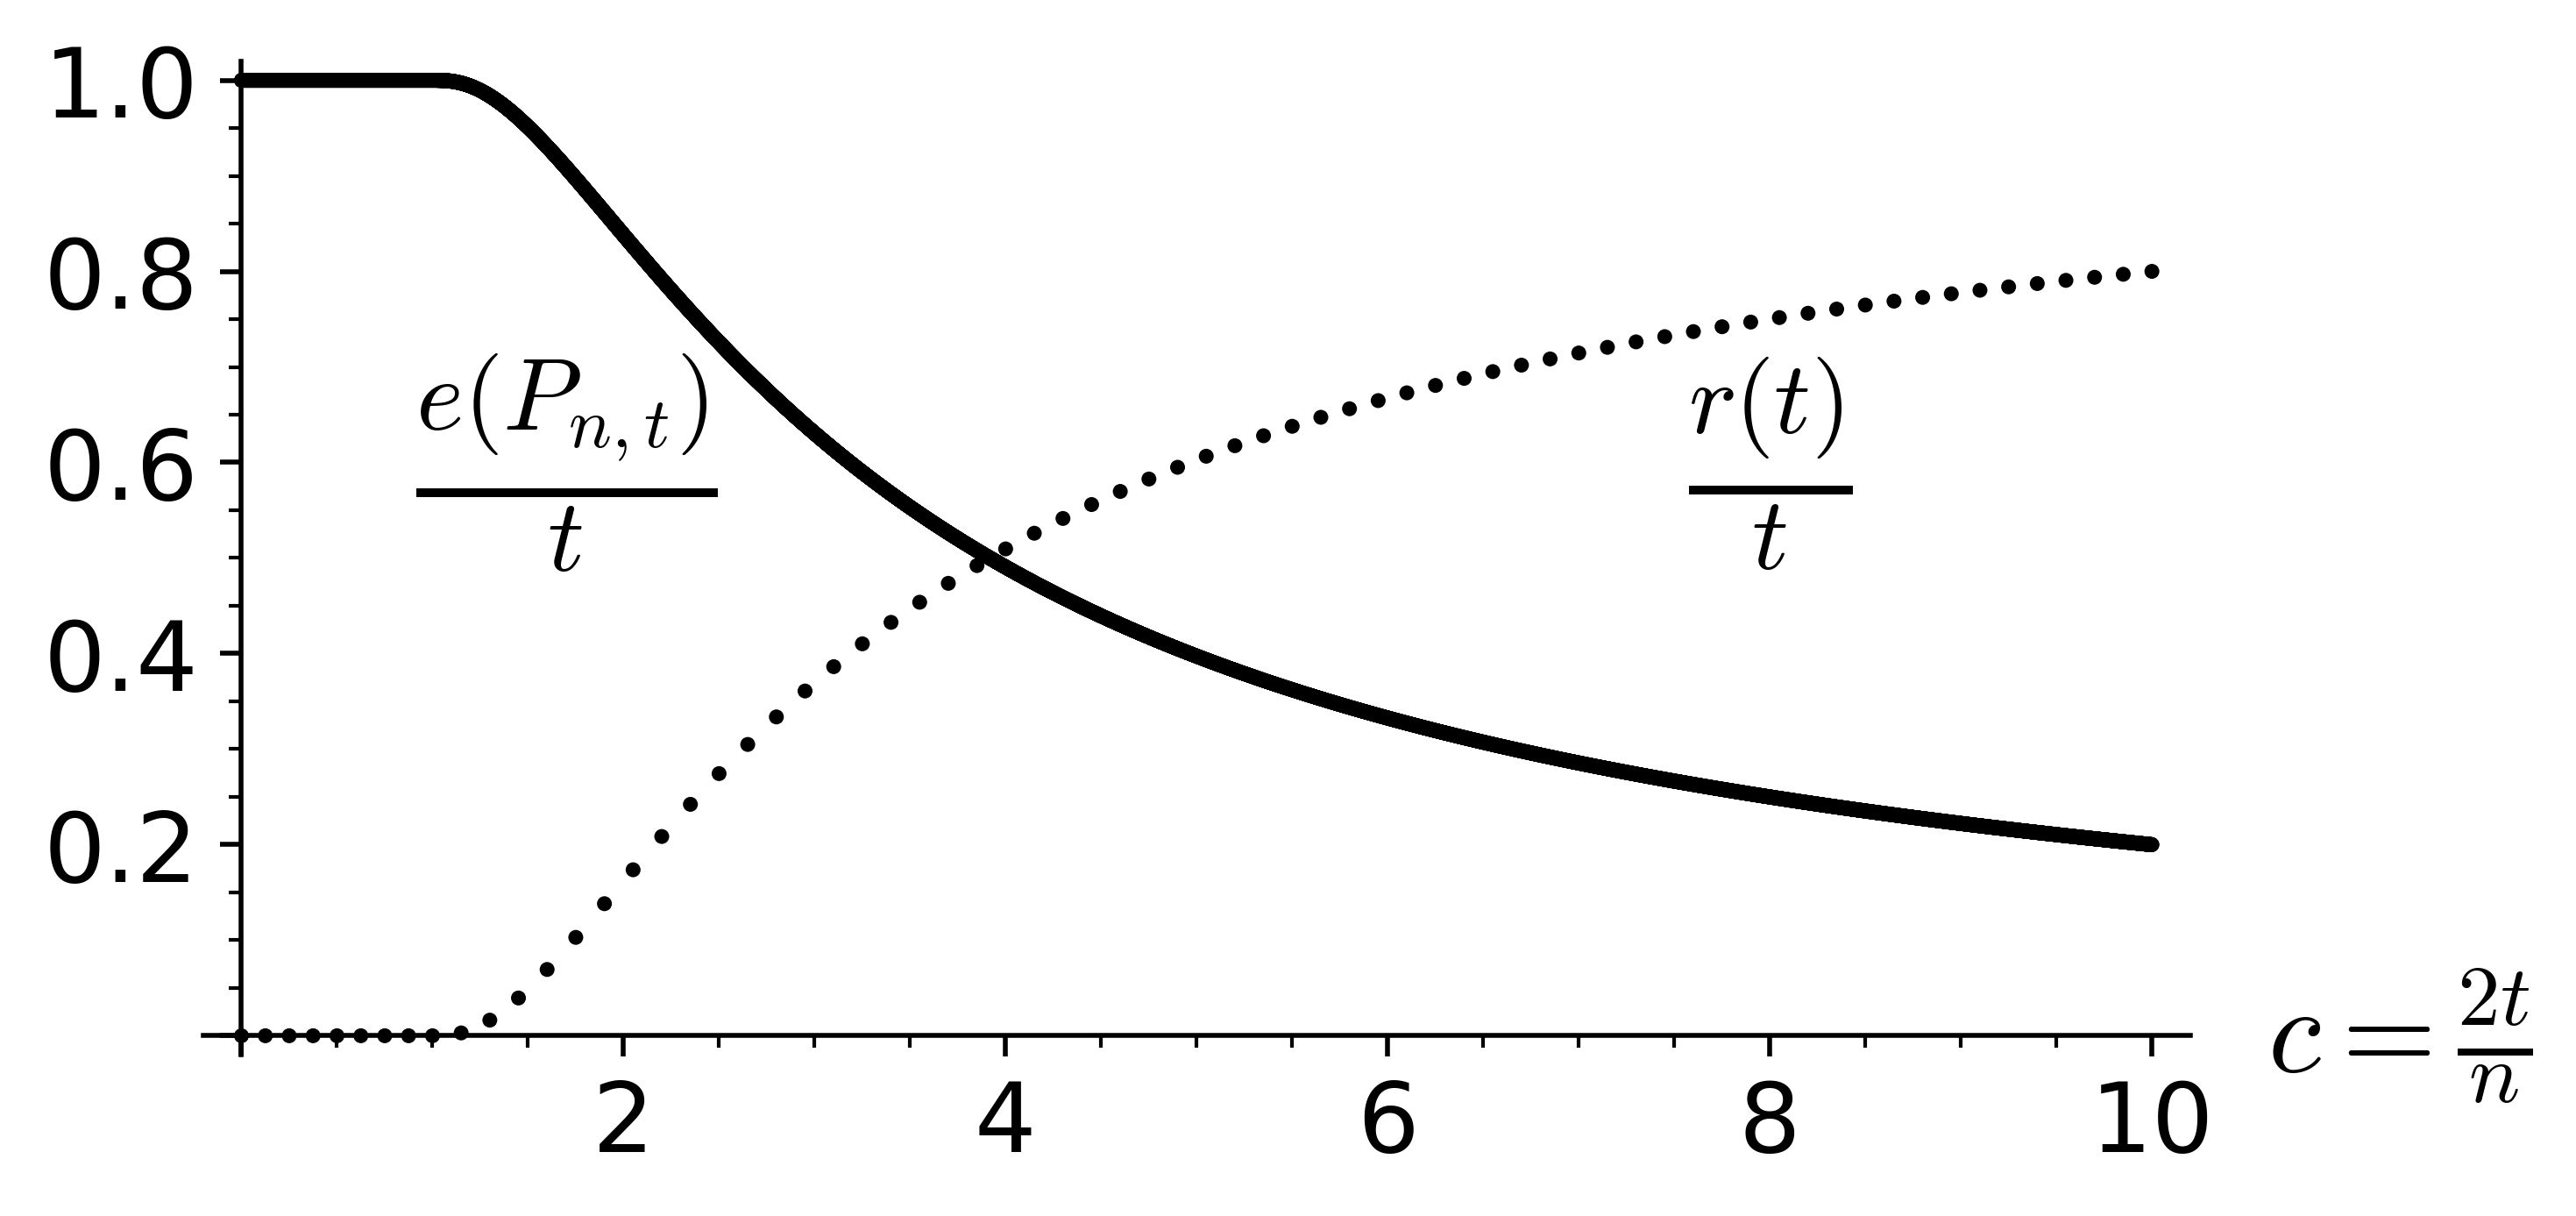
\includegraphics[scale=0.6]{process-fraction.png}
	\caption{The fraction $\numberEdges{\pro{n}{t}}/t$ of edges that are accepted up to step $t=cn/2$ (solid line) and the fraction $\rej{t}/t$ of rejected edges (dotted line). For $c>1$ we have $\numberEdges{\pro{n}{t}}/t\sim \funcPro{c}/c$ and $\rej{t}/t\sim 1-\funcPro{c}/c$.}
	\label{PPfig:fraction}
\end{figure}

We note that in the case $t=cn/2$ for $c>1$ the statement can be simplified to \whp\ $\numberEdges{\pro{n}{t}}=\left(\funcPro{c}+\smallo{1}\right)n/2$. Using \Cref{PPthm:main} we obtain the following nice, alternative description of a $\mathcal{P}$-constrained random graph process: In the very early stage of the process when $t\leq n/2+\smallo{n}$, \lq almost\rq\ all edges are accepted. More formally, \whp\ the \lq next\rq\ edge $e_{t+1}$ will be accepted as long as $t\leq n/2+\smallo{n}$. However, this changes when $t=cn/2$ for $c>1$: The acceptance mainly depends whether or not both of the endpoints of $e_{t+1}$ lie in the largest component of $\pro{n}{t}$.

\begin{coro}\label{PPcoro:main}
Let $\mathcal{P}$ be a class of graphs satisfying the properties \ref{PPdef:classA}--\ref{PPdef:classF} in \Cref{PPdef:class} and $\left(\pro{n}{t}\right)_{t=0}^{N}$ be the $\mathcal{P}$-constrained random graph process. Let $t=t(n)\in\left[N\right]$ be such that $t=cn/2$ for a constant $c>1$, and let $L=\largestcomponent{\pro{n}{t}}$ denote the largest component of $\pro{n}{t}$. Then \whp\ the following hold.
\begin{enumerate}
\item\label{PPcoro:mainA}
If $e_{t+1}\subseteq \vertexSet{\Largestcomponent}$, then $e_{t+1}$ is rejected.
\item\label{PPcoro:mainB}
If $e_{t+1}\nsubseteq \vertexSet{\Largestcomponent}$, then $e_{t+1}$ is accepted.
\end{enumerate}
\end{coro}

Using \Cref{PPthm:main} we can determine the asymptotic number of queried edges $\con{m_0}$ until $m_0$ of them have been accepted in the case $m_0=cn/2$ for $1<c<2$. In particular, this answers the open problem on $\con{3n/4}$ for the property $\mathcal{P}$ of being planar from \cite{GerkeSchlatterStegerTaraz2008}.

\begin{coro}\label{PPcoro:considered}
	Let $\mathcal{P}$ be a class of graphs satisfying the properties \ref{PPdef:classA}--\ref{PPdef:classF} in \Cref{PPdef:class} and $\con{m_0}$ be as defined in \eqref{PPeq:10}. If $m_0=cn/2$ for a constant $c\in(1,2)$, then \whp
	\begin{align*}
		\con{m_0}=\left(\invFunc{c}+\smallo{1}\right)n/2.
	\end{align*}
	In particular, \whp\ $\con{3n/4}=\left(\invFunc{3/2}+\smallo{1}\right)n/2$, where $\invFunc{3/2}=1.6188\ldots$.
\end{coro}

We note that \Cref{PPcoro:considered} follows directly from \Cref{PPthm:main} and the observation that $f$ is strictly increasing (see \Cref{PPlem:function}\ref{PPlem:functionB}).

Our next main result provides the asymptotic order of the largest component of $\acc{n}{m_0}$.

\begin{thm}\label{PPthm:largestComponent}
	Let $\mathcal{P}$ be a class of graphs satisfying the properties \ref{PPdef:classA}--\ref{PPdef:classF} in \Cref{PPdef:class} and $\left(\pro{n}{t}\right)_{t=0}^{N}$ be the $\mathcal{P}$-constrained random graph process. Let $m_0=m_0(n)\in\left[N\right]$ and $s=s(n)$. Let $\acc{n}{m_0}$ be defined as in \eqref{PPeq:9} and let $\numberVertices{\largestcomponent{\acc{n}{m_0}}}$ denote the number of vertices in the largest component of $\acc{n}{m_0}$. Then \whp
	\begin{align*}
		\numberVertices{\largestcomponent{\acc{n}{m_0}}}=
		\begin{cases}
			\bigo{\log n} & \text{if} ~ m_0=cn/2 ~\text{for}~ c<1;
			\\
			\left(1/2+\smallo{1}\right)n^2/s^2\log\left(s^3/n^2\right) & \text{if} ~ m_0=n/2-s \hspace{0.09cm}\text{for}~ n^{2/3}\ll s\ll n;
			\\
			\Th{n^{2/3}}& \text{if} ~ m_0=n/2+s ~\text{for}~ s=\bigo{n^{2/3}};
			\\
			\left(4+\smallo{1}\right)s& \text{if} ~ m_0=n/2+s \hspace{0.09cm}\text{for}~ n^{2/3}\ll s\ll n;
			\\
			\left(\sol{\invFunc{c}}+\smallo{1}\right)n& \text{if} ~ m_0=cn/2 ~\text{for}~ 1<c<2;
			\\
			\left(1+\smallo{1}\right)n& \text{if} ~ m_0=cn/2 ~\text{for}~ c=2;
			\\
			n& \text{if} ~ m_0=cn/2 ~\text{for}~ c>2.
		\end{cases}
	\end{align*}
\end{thm}

For the property $\mathcal{P}$ of being planar \Cref{PPthm:largestComponent} reveals a different behaviour of $\acc{n}{m_0}$ in the \lq sparse\rq\ regime than that of the uniform random planar graph $P(n,m_0)$. More formally, if $m_0=cn/2$ for $1<c<2$, then \whp
\begin{align}\label{PPeq:11}
\numberVertices{\largestcomponent{\acc{n}{m_0}}}=\left(\sol{\invFunc{c}}+\smallo{1}\right)n>\left(c-1+\smallo{1}\right)n=\numberVertices{\largestcomponent{P(n,m_0)}},
\end{align}
where the last equality follows from \cite{KangLuczak2012}. We refer to \Cref{PPfig:cv} for an illustration of $\numberVertices{\largestcomponent{\acc{n}{m_0}}}$ and $\numberVertices{\largestcomponent{P(n,m_0)}}$.




\begin{figure}[t]
\centering
	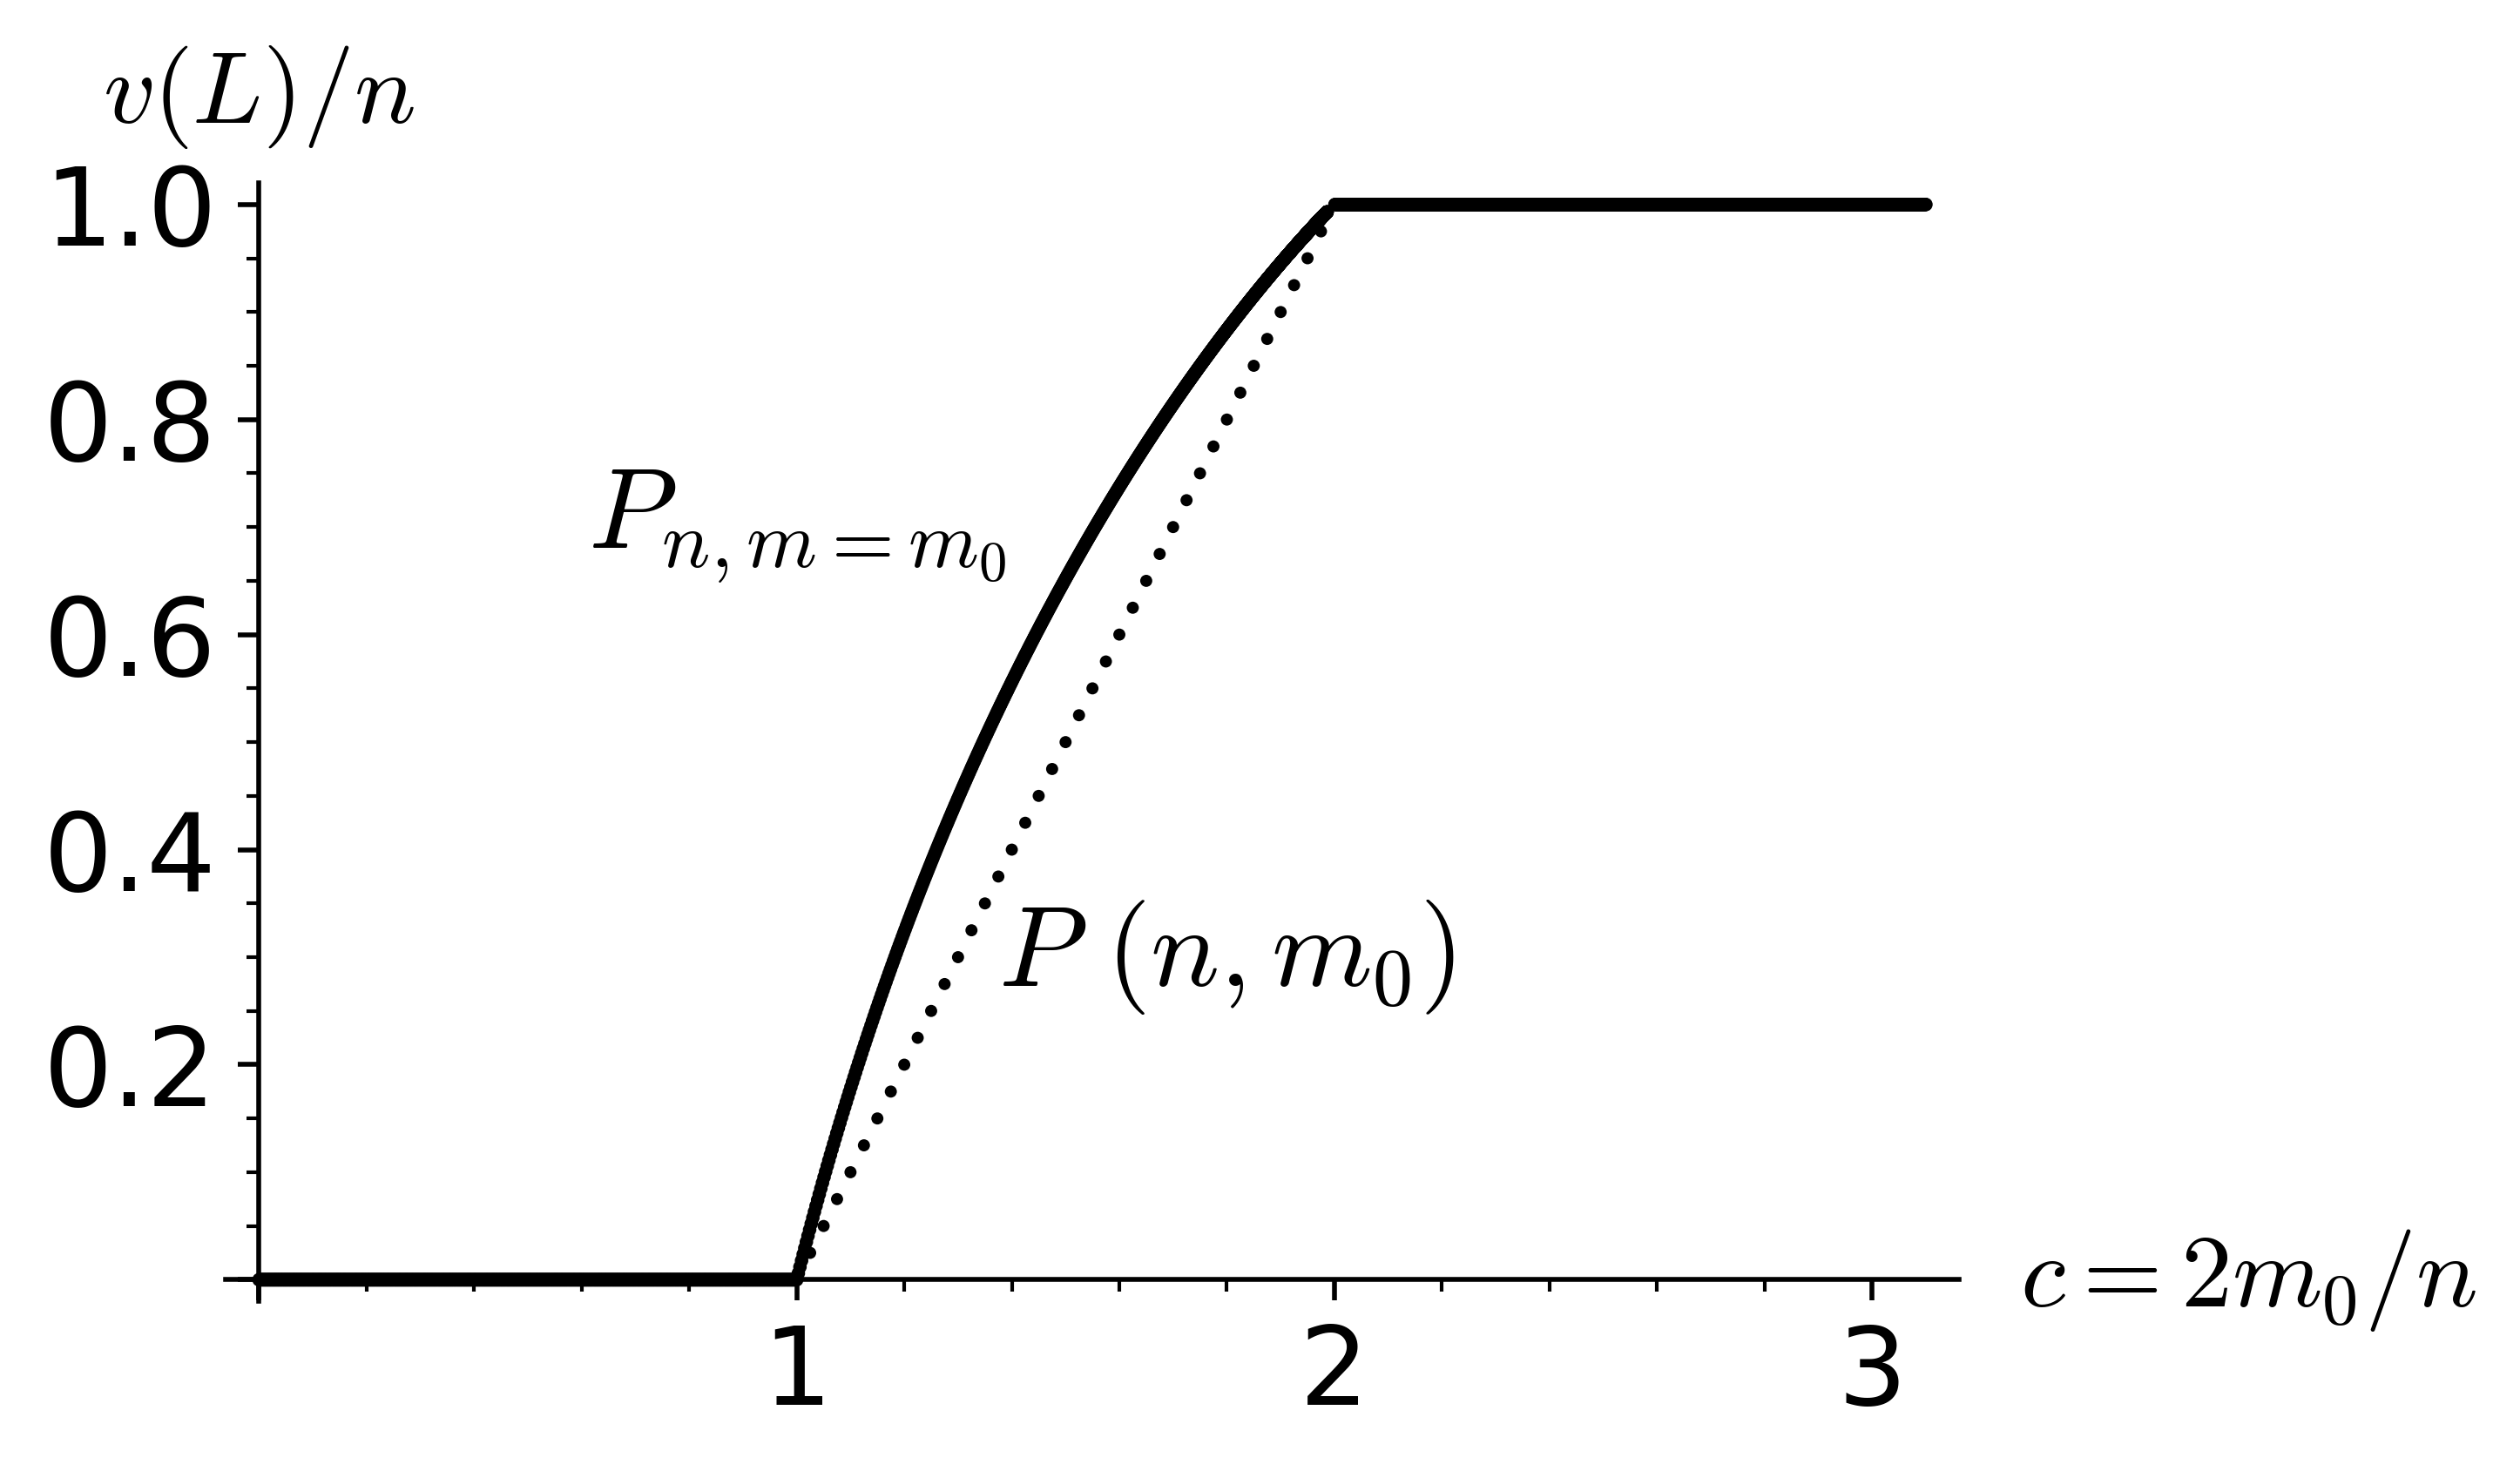
\includegraphics[scale=0.535]{process-largest_component.png}
	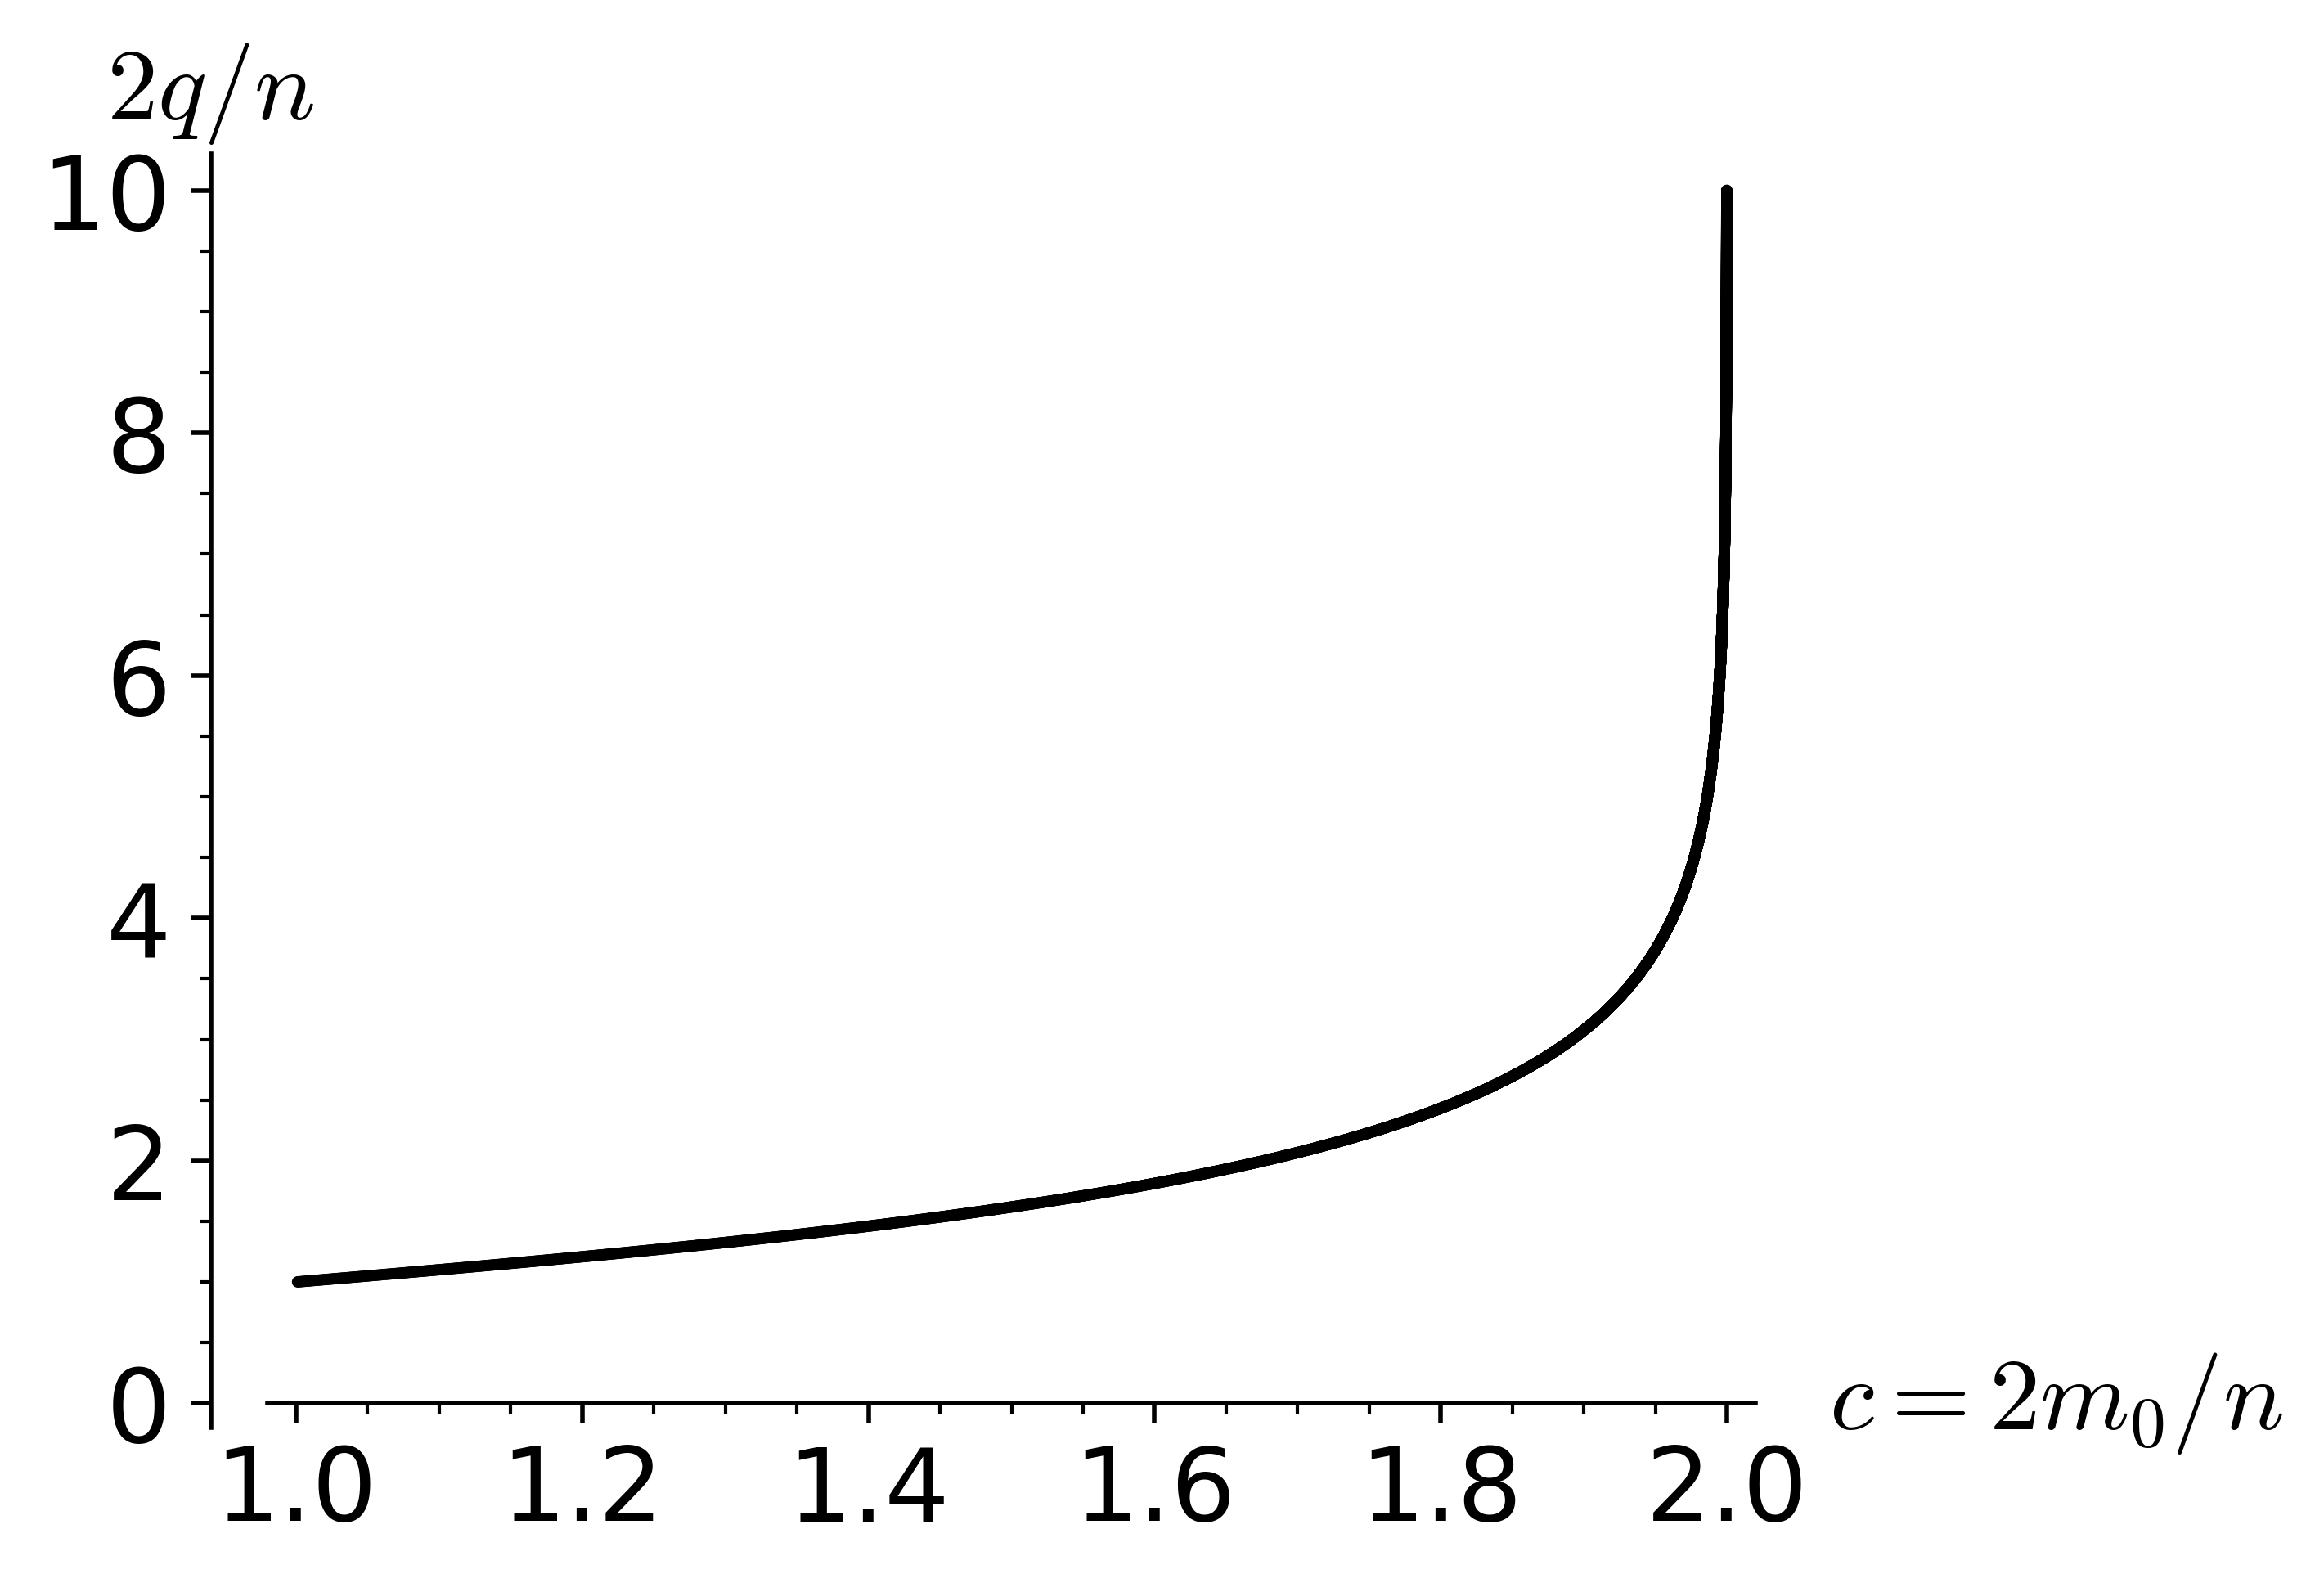
\includegraphics[scale=0.465]{process-considered.png}
	\caption{On the left-hand side: the fraction of vertices lying in the largest component of $\acc{n}{m_0}$ (solid line) and in the uniform random planar graph $P(n,m_0)$ (dotted line) are shown. For $1<c<2$ we have $\numberVertices{\largestcomponent{\acc{n}{m_0}}}/n\sim \sol{\invFunc{c}}$ and $\numberVertices{\largestcomponent{P(n,m_0)}}/n\sim c-1$. On the right-hand side: $2\con{m_0}/n\sim f^{-1}(c)$ is illustrated for the case that $m_0=cn/2$ for $c\in(1,2)$. }
	\label{PPfig:cv}
\end{figure}

\subsection{Outline of the paper}
The rest of the paper is structured as follows. After providing the necessary definitions and concepts in \Cref{PPsec:preliminaries}, we prove \Cref{PPthm:main} in \Cref{PPsec:proof_main}. In \Cref{PPsec:proof_coro} we use so-called \lq addable\rq\ and \lq forbidden\rq\ edges to prove \Cref{PPcoro:main}. Subsequently in \Cref{PPsec:accepted_graph}, we prove \Cref{PPthm:largestComponent}. Finally in \Cref{PPsec:propertiesF}, we consider the function $f$ defined in \Cref{PPdef:func}.

\section{Preliminaries}\label{PPsec:preliminaries}
\subsection{Notations for graphs}
We begin with some notations for graphs that will be used in the rest of the paper.
\begin{definition}
	Given a graph $H$ we denote by
	\begin{itemize}
		\item 
		$\vertexSet{H}$ the vertex set of $H$ and
		\item[]
		$\numberVertices{H}$ the order of $H$, i.e., the number of vertices in $H$;
		\item 
		$\edgeSet{H}$ the edge set of $H$ and
		\item[]
		$\numberEdges{H}$ the size of $H$, i.e., the number of edges in $H$;	
		\item
		$\maxdegree{H}$ the maximum degree of $H$;
		\item 
		$\largestcomponent{H}$ the largest component of $H$;
		\item
		$\core{H}$ the 2-core of $H$, which is the maximal subgraph of $H$ with minimum degree at least two;
		\item
		$\ex{H}:=\numberEdges{H}-\numberVertices{H}+\nt{H}$ the excess of $H$, where $\nt{H}$ is the number of tree components in $H$.
	\end{itemize}
\end{definition}
\begin{definition}\label{PPdef:graph_class}
	Given a class $\mathcal{P}$ of graphs, we write
	$\mathcal{P}(n)$ for the subclass of $\mathcal{P}$ containing the graphs on vertex set $[n]$ 
	and $\mathcal{P}(n,m)$ for the subclass of $\mathcal{P}$ containing the graphs on vertex set $[n]$ with $m$ edges, respectively.
\end{definition}


\subsection{Properties of the \ER\ random graph}
In this section we state the properties of the \ER\ random graph $\er{n}{t}$ which we will use in our proofs. First we consider the case $t=n/2+s$ for $n^{2/3}\ll s\ll n$ and then the case $t=cn/2$ for $c>1$.
\begin{thm}[\hspace{1sp}\cite{Bollobas1982,Luczak1990,Luczak1991b,Pavlov1977}]\label{PPthm:er}
	Let $t=t(n)\in\left[N\right]$ and $s=s(n)$ be such that $t=n/2+s$ for $n^{2/3}\ll s\ll n$ and $\Largestcomponent=\largestcomponent{\er{n}{t}}$ be the largest component of the \ER\ random graph $\er{n}{t}$. Furthermore, let $C=\core{L}$ be the 2-core of $\Largestcomponent$ and $F$ be the forest obtained from $L$ by deleting the edges of $C$. Then \whp
	\begin{enumerate}
		\item\label{PPthm:erA}
		$\numberVertices{\Largestcomponent}=\left(4+\smallo{1}\right)s$;
		\item\label{PPthm:erE}
		$\ex{\er{n}{t}}=\Th{s^3/n^2}$;
		\item\label{PPthm:erB}
		each tree component of $F$ is of order $\smallo{s}$;
		\item\label{PPthm:erC}
		$\maxdegree{\er{n}{t}}=\left(1+\smallo{1}\right)\log n/\log\log n$;
		\item\label{PPthm:erD}
		$\maxdegree{C}=3$ if in addition $s\ll n^{3/4}$.
	\end{enumerate}
\end{thm}

We note that \ref{PPthm:erA} and \ref{PPthm:erE} are shown in \cite{Luczak1990}, \ref{PPthm:erC} in \cite{Bollobas1982}, and \ref{PPthm:erD} in \cite{Luczak1991b}, respectively. Furthermore, \ref{PPthm:erB} follows by the fact from \cite{Pavlov1977} that conditioned on fixed values of $\numberVertices{\Largestcomponent}$ and $\numberVertices{C}$, \whp\ all tree components of $F$ are of order $\smallo{\numberVertices{\Largestcomponent}}$ as long as $\numberVertices{C}^2=\smallomega{\numberVertices{\Largestcomponent}}$. Furthermore, \whp\ $\er{n}{t}$ satisfies this condition, because \whp\ $\numberVertices{C}=\Th{s^2/n}$ by \cite{Luczak1991b} and $\numberVertices{\Largestcomponent}=\left(4+\smallo{1}\right)s$ by \ref{PPthm:erA}.

Next we collect some properties of the \ER\ random graph $\er{n}{t}$ when $t=cn/2$ for $c>1$.


\begin{thm}[\hspace{1sp}\cite{ErdoesRenyi1960}]\label{PPthm:erInt}
	Let $t=t(n)\in\left[N\right]$ be such that $t=cn/2$ for $c>1$. Let $G=\er{n}{t}$ be the \ER\ random graph, and $\Largestcomponent=\largestcomponent{G}$ the largest component of $G$. Furthermore, let $\sol{c}$ and $\funcPro{c}$ be as in \Cref{PPdef:func}. Then \whp
	\begin{enumerate}
		\item\label{PPthm:erIntA}
		$\numberVertices{\Largestcomponent}=\left(\sol{c}+\smallo{1}\right)n$;
		\item\label{PPthm:erIntC}
		all components of $G$ apart from $L$ are of order $\smallo{n}$;
		\item\label{PPthm:erIntB}
		$\ex{G}=\left(c-\funcPro{c}+\smallo{1}\right)n/2$.
	\end{enumerate}
\end{thm}

\subsection{Basic properties of the random planar graph process}
We will often use the following simple observation.
\begin{remark}\label{PPrem:component_structure}
Due to properties \ref{PPdef:classB} and \ref{PPdef:classE} of \Cref{PPdef:class} there is a path between two vertices in $\pro{n}{t}$ if and only if there is one in $\er{n}{t}$.
\end{remark}

Next, we show that the number of rejected edges up to step $t$ is bounded above by the excess of $\er{n}{t}$. This will be a main ingredient to obtain the upper bounds in \Cref{PPthm:main}.

\begin{lem}\label{PPlem:upperBound_excess}
For all $t\in \left[N\right]$ we have
\begin{align*}
\rej{t}\leq \ex{\er{n}{t}}.
\end{align*}
\end{lem}

\begin{proof}
We consider an edge $e_i$ which is rejected in the $\mathcal{P}$-constrained random graph process. By \Cref{PPdef:class}\ref{PPdef:classE} and \ref{PPdef:classF} the two endpoints of $e_i$ lie in the same component of $\pro{n}{i-1}$, which is not a tree component. Together with the fact $\pro{n}{i-1}\subseteq \er{n}{i-1}$ it implies that adding $e_i$ to $\er{n}{i-1}$ increases the excess by one, i.e., $\ex{\er{n}{i}}=\ex{\er{n}{i-1}}+1$. As $\ex{\er{n}{t}}$ is non-decreasing in $t$, this implies the statement.
\end{proof}

A graph class $\mathcal{A}$ for which there exists a constant $c>0$ such that $\left|\mathcal{A}(n)\right|\leq n!c^n$ for all $n\in\N$ is often called \textit{small} (see e.g., \cite{NorineSeymourThomasWollan2006}). The following statement shows that the class $\mathcal{P}$ in \Cref{PPdef:class} is small.
\begin{thm}[\hspace{1sp}\cite{NorineSeymourThomasWollan2006}]\label{PPthm:small_classes}
	Let $\mathcal{P}$ be a class of graphs satisfying the properties \ref{PPdef:classA}, \ref{PPdef:classC}, and \ref{PPdef:classD} in \Cref{PPdef:class}. Then there exists a constant $c>0$ such that $\left|\mathcal{P}(n)\right|\leq n!c^n$ for all $n\in\N$. 
\end{thm}

\subsection{Decomposition of graphs}
In the proof of \Cref{PPthm:main} we will decompose the largest component of $\pro{n}{t}$ into connected parts of roughly equal size. To that end, we will use the following lemma, which is an extension of \cite[Proposition 4.5]{KrivelevichNachmias2006} to vertex-weighted graphs.
\begin{lem}\label{PPlem:decomposition}
Let $H$ be a connected graph with maximum degree at most $\Delta\geq 1$. We assign each vertex $x\in\vertexSet{H}$ a vertex-weight $\weight{x}>0$. Assume that $\max_{x\in\vertexSet{H}}\weight{x}\leq M$ for some $M>0$. Then, given $a>0$ there exist disjoint vertex sets $V_1, \ldots, V_r\subseteq \vertexSet{H}$ such that
\begin{itemize}
\item
$H\left[V_i\right]$ is connected for each $i\in[r]$;
\item
$a\leq W_i\leq a \Delta+M$ for each $i\in[r]$;
\item
$W(H)-\sum_{i=1}^{r}W_i<a$,
\end{itemize}
where $W(H):=\sum_{x\in V(H)}\weight{x}$ is the total vertex-weight of $H$ and $W_i:=\sum_{x\in V_i}\weight{x}$ the total vertex-weight of $V_i$, respectively.
\end{lem}

\begin{proof}
We proceed by induction on $\numberVertices{H}$. For $\numberVertices{H}=1$ let $x$ denote the single vertex in $H$. We set $V_1=\left\{x\right\}$ if $\weight{x}\geq a$ and let $r=0$ otherwise.
 
Now assume $\numberVertices{H}>1$. If $W(H)<a$, we set $r=0$. Assume otherwise that $W(H)\geq a$. We perform a breadth-first search (BFS) starting at some arbitrary vertex $y$. For each vertex $x\in\vertexSet{H}$ let $D_x$ be the set of vertices consisting of $x$ and all descendants of $x$ in the BFS-tree and let $W(x):=\sum_{u\in D_x}\weight{u}$ be the total vertex-weight of $D_x$. Let $z\in \vertexSet{H}$ be the vertex such that $W(z)$ is minimal among all vertices $x$ with $W(x)\geq a$. We note that such a vertex exists, as $W(y)=W(H)\geq a$. Let $z_1, \ldots, z_k$ be the neighbours of $z$ that are contained in $D_z$. By minimality of $z$ we have $W(z_i)<a$ for all $i\in[k]$. Thus, we get $W(z)=\sum_{i=1}^{k}\weight{z_i}+\weight{z}\leq a\Delta +M$. Therefore, we choose $V_1=D_z$. By construction $H\left[V_1\right]$ is connected and we have $a\leq W_1\leq a \Delta+M$. Furthermore, the graph obtained from $H$ by deleting $V_1$ is connected and has less vertices than $H$. Hence, we can apply the induction hypothesis to this graph to obtain the remaining sets $V_2, \ldots, V_r$ of our desired decomposition.
\end{proof}

We will show that if we have a \lq suitable\rq\ decomposition of $\pro{n}{t}$, we cannot add too \lq many\rq\ further edges without creating a minor of the complete graph $K_\ell$ for an appropriate $\ell\in\N$. To that end, we will use the following lemma, which is a \lq weighted\rq\ version of the well-known Tur{\'a}n's theorem.
\begin{lem}\label{PPlem:weighted_turan}
For fixed $n\in\N$ we assign a vertex-weight $\weight{x}>0$ to each vertex $x$ of $K_n$. Furthermore, we define the edge-weight $\weight{xy}:=\weight{x}\weight{y}$ for each edge $xy\in\edgeSet{K_n}$. Let $S_n:=\sum_{x\in\vertexSet{K_n}}\weight{x}$ be the total vertex-weight of $K_n$ and $M_n:=\max_{x\in\vertexSet{K_n}}\weight{x}$ be the maximum vertex-weight of $K_n$. For each subgraph $H\subseteq K_n$ denote by $\weight{H}:=\sum_{e\in \edgeSet{H}}\weight{e}$ the total edge-weight of $H$. Then for each $\ell\geq 2$ we have 
\begin{align*}
\weight{K_n}-\max\setbuilder{\weight{H}}{H\subseteq K_n, K_\ell\nsubseteq H}\geq \frac{S_n}{2}\left(\frac{S_n}{\ell-1}-M_n\right).
\end{align*}
\end{lem}
\begin{proof}
To ease notation, let $A_n:=\max\setbuilder{\weight{H}}{H\subseteq K_n, K_\ell\nsubseteq H}$. In \cite{BennettEnglishTalanda-Fisher2019} Bennett, English, and Talanda-Fisher showed that
\begin{align*}
A_n=\frac{1}{2} \cdot\max_{\mathcal{Q}}\sum_{Q\neq Q'\in\mathcal{Q}}W(Q)W\left(Q'\right),
\end{align*}
where the maximum is taken over all partitions $\mathcal{Q}$ of $\vertexSet{K_n}$ into $\ell-1$ parts and $W(Q):=\sum_{x\in Q}\weight{x}$ denotes the total vertex-weight of $Q\in\mathcal{Q}$. Now let $\mathcal{Q}^\ast$ be some partition for which the maximum is attained. Note that $\sum_{Q\in\mathcal{Q}^\ast}W(Q)=\sum_{x\in\vertexSet{K_n}}\weight{x}=S_n$. Furthermore, we have
\begin{align*}
A_n~&=~\frac{1}{2}\sum_{Q\neq Q'\in\mathcal{Q}^\ast}W(Q)W\left(Q'\right)~=~\frac{1}{2} \left(\sum_{Q\in\mathcal{Q}^\ast}W(Q)\right)^2-\frac{1}{2}\sum_{Q\in\mathcal{Q}^\ast}W(Q)^2~
\\
&=~\frac{S_n^2}{2}-\frac{1}{2}\sum_{Q\in\mathcal{Q}^\ast}W(Q)^2.
\end{align*}
Using the \lq AM-QM inequality\rq, in other words, $\sum_{Q\in\mathcal{Q}^\ast}W(Q)^2\geq \frac{1}{\ell-1}\left(\sum_{Q\in\mathcal{Q}^\ast}W(Q)\right)^2$, we obtain
\begin{align}\label{PPeq:2}
A_n~\leq~\frac{S_n^2}{2}-\frac{1}{2}\cdot \frac{1}{\ell-1}\left(\sum_{Q\in\mathcal{Q}^\ast}W(Q)\right)^2~=~ \frac{S_n^2}{2}\left(1-\frac{1}{\ell-1}\right).
\end{align}
Finally, the total edge-weight of $K_n$ satisfies
\begin{align*}
	\weight{K_n}~&=~\sum_{e\in\edgeSet{K_n}}\weight{e}~=~\frac{1}{2}\sum_{x\neq y\in\vertexSet{K_n}}\weight{x}\weight{y}
	\\
	&=~\frac{S_n^2}{2}-\frac{1}{2}\sum_{x\in\vertexSet{K_n}}\weight{x}^2~\geq~ \frac{S_n^2}{2}-\frac{S_nM_n}{2}.
\end{align*}
This together with \eqref{PPeq:2} implies the statement.
\end{proof}



\section[Rejected edges]{Rejected edges: Proof of \Cref{PPthm:main}}\label{PPsec:proof_main}
The upper bounds follow immediately from \Cref{PPlem:upperBound_excess}.

\subsection{Proof of upper bounds}\label{PPsubsec:proofUpper}
Due to \cite{Britikov1989,JansonKnuthLuczakPittel1993} and \Cref{PPthm:er}\ref{PPthm:erE} and \ref{PPthm:erInt}\ref{PPthm:erIntB} we have that \whp
\begin{align*}
	\ex{\er{n}{t}}=
	\begin{cases}
		0 & \text{if} ~~ t=n/2-s ~~\text{for}~~ s\gg n^{2/3};
		\\
		\bigo{h}& \text{if} ~~ t=n/2+s ~~\text{for}~~ s=\bigo{n^{2/3}};
		\\
		\Th{s^3/n^2}& \text{if} ~~ t=n/2+s ~~\text{for}~~ n^{2/3}\ll s\ll n;
		\\
		\left(c-\funcPro{c}+\smallo{1}\right)n/2& \text{if} ~~ t=cn/2 ~~\text{for}~~ c>1.
	\end{cases}
\end{align*}
Together with \Cref{PPlem:upperBound_excess} this implies the upper bounds in \Cref{PPthm:main}. 

Before proving the lower bounds we first sketch the main ideas.

\subsection{Proof idea for lower bounds}\label{PPsubsec:proofidea}
First we consider the case $t=n/2+s$ for $n^{2/3}\ll s\ll n$. We use a consequence of the properties \ref{PPdef:classA} and \ref{PPdef:classD} in \Cref{PPdef:class} that there exists an $\ell\in\N$ such that no graph in $\mathcal{P}$ contains the complete graph $K_\ell$ as a minor. We then apply a \lq sprinkling\rq\ type argument: Let $P=\pro{n}{t}$ and let $P'=\pro{n}{t'}$ for $t'=n/2+s/2$. We first reveal the edges $e_1, \ldots, e_{t'}$. Given the realisation of $P'$, we split the vertex set $\vertexSet{\largestcomponent{P'}}$ of the largest component of $P'$ into disjoint sets $V_1, \ldots, V_r$ of \lq almost\rq\ equal sizes such that $P'\left[V_i\right]$ is connected for each $i\in[r]$, where $r\geq \ell$. Next we reveal the remaining edges $e_{t'+1}, \ldots, e_t$ up to step $t$ and show that for each pair $i\neq j$ there are \lq many\rq\ edges between $V_i$ and $V_j$ which are queried up to step $t$. As $K_\ell$ is not a minor of $P'$, there are some pairs for which all of these edge are rejected. This provides a lower bound on the number of rejected edges. The precise way of decomposing the largest component of $P'$ differs in the cases $s\ll n^{3/4}$ and $s\gg n^{17/24}$. We note that it is sufficient to deal with these two cases, because the general case $n^{2/3}\ll s\ll n$ follows by considering appropriate subsequences.

The starting point for the case $t=cn/2$ for $c>1$ is \Cref{PPthm:small_classes}. Roughly speaking, it says that only a very small number of all graphs on $n$ vertices lie in $\mathcal{P}(n)$. Using that we show that for each $\delta>0$, \whp\ there is no graph $H\in\mathcal{P}\left(n, \left(1+\delta\right)n\right)$ such that all edges of $H$ are already queried before step $\bar{t}:=n \cdot \log n$. In particular, this shows that \whp\ $\numberEdges{\pro{n}{\bar{t}}}\leq \left(1+\smallo{1}\right)n$. It is well known that \whp\ $\er{n}{\bar{t}}$ and therefore also $\pro{n}{\bar{t}}$ are connected. Thus, we obtain that \whp\ $\ex{\pro{n}{t}}\leq \ex{\pro{n}{\bar{t}}}=\smallo{n}$. Furthermore, we have that
\begin{align*}
t-\numberEdges{\pro{n}{t}}=\numberEdges{\er{n}{t}}-\numberEdges{\pro{n}{t}}\geq \ex{\er{n}{t}}-\ex{\pro{n}{t}}.
\end{align*}
Hence, we obtain a lower bound by using that \whp\ $\ex{\pro{n}{t}}=\smallo{n}$ and $\ex{\er{n}{t}}=\left(c-\funcPro{c}+\smallo{1}\right)n/2$ from \Cref{PPthm:erInt}\ref{PPthm:erIntB}.


\subsection{Proof of lower bounds}\label{PPsubsec:proofLower}
(i) We start with the case $t=n/2+s$ for $n^{2/3}\ll s\ll n$. 

Take $t'=n/2+s/2$ and let $P'=\pro{n}{t'}$, $G'=\er{n}{t'}$, $P=\pro{n}{t}$, and $G=\er{n}{t}$. Furthermore, let $\largestcomponent{P'}$ and $\largestcomponent{G'}$ be the largest components of $P'$ and $G'$, respectively. 

Due to the properties \ref{PPdef:classA} and \ref{PPdef:classD} in \Cref{PPdef:class}, there exists an $\ell\in\N$ such that there is no graph in $\mathcal{P}$ having the complete graph $K_\ell$ as a minor. Now we distinguish two cases.

\textit{Case 1: $s\ll n^{3/4}$.}
First reveal the edges $e_1, \ldots, e_{t'}$.

Let $C=\core{\largestcomponent{G'}}$ be the 2-core of $\largestcomponent{G'}$ and $\forestPro{G'}$ the forest obtained from $\largestcomponent{G'}$ by deleting the edges of $C$. Moreover, for a vertex $x\in \vertexSet{C}$ let $T_x$ be the tree component of $\forestPro{G'}$ containing $x$. By \Cref{PPdef:class}\ref{PPdef:classB} and \ref{PPdef:classE} we have $\vertexSet{\largestcomponent{P'}}=\vertexSet{\largestcomponent{G'}}$ and $\edgeSet{\largestcomponent{P'}}\subseteq\edgeSet{\largestcomponent{G'}}$; furthermore, each edge of $\forestPro{G'}$ is also contained in $\largestcomponent{P'}$. Thus, there is a connected and spanning subgraph $C'\subseteq C$ such that $\largestcomponent{P'}$ can be obtained by replacing each vertex $x$ in $C'$ by the tree $T_x$. 

We apply \Cref{PPlem:decomposition} to $C'$, where we define the vertex-weight of a vertex $x\in\vertexSet{C'}$ by $\weight{x}:=\left|\vertexSet{T_x}\right|$. Then due to \Cref{PPthm:er}\ref{PPthm:erA}, \ref{PPthm:erB}, and \ref{PPthm:erD}, \whp\ the total vertex-weight of $C'$ satisfies
\begin{align*}
W\left(C'\right):=\sum_{x\in\vertexSet{C'}}\weight{x}=\sum_{x\in\vertexSet{C'}}\left|\vertexSet{T_x}\right|=\numberVertices{\largestcomponent{P'}}=\numberVertices{\largestcomponent{G'}}=(2+\smallo{1})s,
\end{align*}
the maximum vertex-weight of $C'$ satisfies
\begin{align*}
\max_{x\in\vertexSet{C'}}\weight{x}=\max_{x\in\vertexSet{C'}}\left|\vertexSet{T_x}\right|=\smallo{s},
\end{align*}
and the maximum degree of $C'$ is bounded by $\maxdegree{C'}\leq \maxdegree{C}=3$. Assuming this \whp\ event holds, we apply \Cref{PPlem:decomposition} to $C'$ with $\Delta=3$ and $a=M=s/(3\ell)$ and obtain disjoint vertex sets $\tilde{V}_1, \ldots, \tilde{V}_r\subseteq \vertexSet{C'}$ such that
\begin{itemize}
\item
$C'\left[\tilde{V}_i\right]$ is connected for each $i\in[r]$;
\item
$a=s/(3\ell)\leq W_i\leq a\Delta+M=4s/(3\ell)$ for each $i\in[r]$;
\item
$W\left(C'\right)-\sum_{i=1}^{r}W_i<a=s/(3\ell)$,
\end{itemize}
where $W_i:=\sum_{x\in \tilde{V}_i} \weight{x}=\sum_{x\in\tilde{V}_i}\left|\vertexSet{T_x}\right|$. 

For $i\in[r]$ let $V_i$ be the set of vertices that lie in some $T_x$ for a $x\in\tilde{V}_i$. Then $V_1, \ldots, V_r\subseteq\largestcomponent{P'}$ are pairwise disjoint and satisfy the following properties: 
\begin{itemize}
\item
$P'\left[V_i\right]$ is connected for each $i\in[r]$;
\item
$s/(3\ell)\leq |V_i|\leq 4s/(3\ell)$ for each $i\in[r]$;
\item
$\sum_{i=1}^{r}|V_i|\geq \numberVertices{\largestcomponent{P'}}-s/(3\ell)\geq 4s/3$.
\end{itemize}
Note that $\ell\leq r=\Th{1}$. 
Next we reveal the edges $e_{t'+1}, \ldots, e_t$. We claim that \whp\ for each pair $i\neq j\in[r]$ there are at least $A:=s^3/\left(18\ell^2 n^2\right)$ many edges between points in $V_i$ and $V_j$ which have been queried up to step $t$. Assume that for some $i\neq j\in[r]$ this is not the case and let $k\in\left[N\right]$ be such that $t'<k\leq t$. Then in the step of revealing $e_k$ there were at least $|V_i||V_j|-A\geq s^2/\left(10\ell^2\right)$ many edges going between $V_i$ and $V_j$ which had not been queried yet. Hence, we have 
\begin{align*}
\prob{e_k \text{ has one endpoint in }V_i \text{ and one in }V_j}\geq s^2/\left(5\ell^2n^2\right)=:p.
\end{align*}
Letting $X$ be the number of edges going between $V_i$ and $V_j$ that have been queried up to step $t$ it implies
\begin{align}\label{PPeq:1}
\prob{X\leq A}\leq \prob{\binPro{s/2}{p}\leq A}=\bigo{n^2/s^3}=\smallo{1}.
\end{align}
As $r=\Th{1}$ this shows the claim. By the choice of $\ell$ we know that $K_\ell$ is not a minor of $P=\pro{n}{t}$. Hence, there is a pair $i\neq j\in[r]$ such that there is no edge in $P$ going between $V_i$ and $V_j$. Together with the claim this yields that \whp\ at least $A=\Th{s^3/n^2}$ many edges have been rejected up to step $t$. This concludes the case $s\ll n^{3/4}$.

\textit{Case 2: $s\gg n^{17/24}$.}
First we reveal again only the edges $e_1, \ldots, e_{t'}$.

Using \Cref{PPthm:er}\ref{PPthm:erA} and \ref{PPthm:erC} we have that \whp\
\begin{align*}
\numberVertices{\largestcomponent{P'}}&=\numberVertices{\largestcomponent{G'}}=\left(2+\smallo{1}\right)s \quad \text{and}   \\[0.1cm]
\maxdegree{\largestcomponent{P'}}&\leq \maxdegree{G'}=\left(1+\smallo{1}\right)\log n/\log \log n.
\end{align*}
Assuming this \whp\ event holds, we apply \Cref{PPlem:decomposition} to $\largestcomponent{P'}$ where we assign a vertex-weight $\weight{x}=1$ to each $x\in\vertexSet{\largestcomponent{P'}}$, $\Delta=\log n$, $M=1$, and $a=s/(\ell \log n)$. This leads to disjoint sets $V_1, \ldots, V_r \subseteq \vertexSet{\largestcomponent{P'}}$ such that $\largestcomponent{P'}\left[V_i\right]$ is connected for each $i\in[r]$, 
\begin{align}
s/(\ell \log n)&\leq |V_i|\leq s/\ell+1 \quad \text{for each }i\in[r], \quad \text{and}\label{PPeq:3}\\
\sum_{i\in[r]}|V_i|&\geq \largestcomponent{P'}-s/(\ell \log n)=(2+\smallo{1})s. \label{PPeq:4}
\end{align}

Next reveal the remaining edges $e_{t'+1}, \ldots, e_t$. We claim that \whp\ for each pair $i\neq j\in[r]$ there are at least $B:=|V_i||V_j| s/\left(2n^2\right)$ edges that have been queried up to step $t$. To prove the claim, let $i\neq j\in[r]$ be fixed and denote by $X$ the number of edges between $V_i$ and $V_j$ that have been queried up to step $t$. Analogous to \eqref{PPeq:1} we obtain, with $q:=3|V_i||V_j|/\left(2n^2\right)$,
\begin{align*}
\prob{X\leq B}\leq \prob{\binPro{s/2}{q}\leq B}=\bigo{\frac{n^2}{|V_i||V_j|s}}=\bigo{\frac{n^2 \log n^2}{s^3}}=\smallo{n^{-1/9}},
\end{align*}
where we used Chebyshev's inequality, \eqref{PPeq:3}, and $s\gg n^{17/24}$. As $r=\bigo{\log n}$, the claim follows by the union bound. Next, let $H$ be the graph with (super)vertex set $\vertexSet{H}=\left\{V_1, \ldots, V_r\right\}$ and two vertices $V_i$ and $V_j$ are connected if and only if there is an edge in $P$ going between $V_i$ and $V_j$. We assign each vertex $V_i$ in $H$ the vertex-weight $w(V_i):=|V_i|$. Due to \eqref{PPeq:3} and \eqref{PPeq:4} we have that the maximum vertex-weight and the total vertex-weight of $\vertexSet{H}$ satisfy 
\begin{align*}
M_r:=\max_{i\in[r]}\weight{V_i}\leq s/\ell+1 \quad \text{ and } \quad S_r:=\sum_{i\in[r]}\weight{V_i}=(2+\smallo{1})s.
\end{align*}
Let $I$ be the set of unordered pairs $i\neq j$ such that there is no edge in $H$ going between $V_i$ and $V_j$. We note that $K_\ell\nsubseteq H$, as $K_\ell$ is not a minor of $P$. Then by \Cref{PPlem:weighted_turan} we obtain
\begin{align*}
\sum_{\left\{i,j\right\}\in I}|V_i||V_j|\geq \frac{S_r}{2}\left(\frac{S_r}{\ell-1}-M_r\right)=\Th{s^2}.
\end{align*}
By definition of $I$ there is no edge in $P$ going between $V_i$ and $V_j$ for each unordered pair $\left\{i,j\right\}\in I$. Furthermore, \whp\ for each of these pairs at least $B=|V_i||V_j| s/\left(2n^2\right)$ many edges between $V_i$ and $V_j$ have been queried up to step $t$. Thus, the number of rejected edges satisfies that \whp 
\begin{align*}
\rej{t}\geq \frac{s}{2n^2} \sum_{\left\{i,j\right\}\in I}|V_i||V_j|\geq \Th{s^3/n^2}.
\end{align*}
This concludes the case $s\gg n^{17/24}$ and therefore also the case $t=n/2+s$ for $n^{2/3}\ll s\ll n$.

(ii) We consider the case where $n=cn/2$ for $c>1$. Let $\bar{t}:=n \cdot \log n$, $\bar{P}:=\pro{n}{\bar{t}}$, and $P:=\pro{n}{t}$. We claim that \whp\
\begin{align}\label{PPeq:5}
	\numberEdges{\bar{P}}\leq \left(1+\smallo{1}\right)n.
\end{align}
To show the claim, we use an idea from \cite{GerkeSchlatterStegerTaraz2008}: Let $\delta>0$, $m:=(1+\delta)n$, $H\in\mathcal{P}(n,m)$, and $\edgeSet{H}=\left\{f_1, \ldots, f_m\right\}$. We have
\begin{align*}
\prob{H\subseteq\bar{P}}
~&\leq~\prob{\left\{f_1, \ldots, f_m\right\}\subseteq\left\{e_1, \ldots, e_{\bar{t}}\right\}}
~\leq~\prod_{i=1}^{m}\prob{f_i\in \left\{e_1, \ldots, e_{\bar{t}}\right\}}
\\
&=~\left(\frac{\bar{t}}{N}\right)^m
~=~\left(\frac{2\log n}{n-1}\right)^m.
\end{align*}
By \Cref{PPthm:small_classes} there exists a $c>0$ such that $\left|\mathcal{P}(n)\right|\leq n!c^n$ for all $n\in\N$. Thus, we obtain by taking the union bound
\begin{align*}
\prob{\numberEdges{\bar{P}}\geq m}&~\leq~ \left|\mathcal{P}(n)\right|\left(\frac{2\log n}{n-1}\right)^m
~\leq~
n!c^n\left(\frac{2\log n}{n-1}\right)^m
\\
&~\leq~
n^nc^n\left(\frac{2\log n}{n-1}\right)^m
~=~
\left(\frac{nc\left(2\log n\right)^{1+\delta}}{\left(n-1\right)^{1+\delta}}\right)^n
~=~\smallo{1},
\end{align*}
which gives \eqref{PPeq:5}. Next we use the well-known fact that \whp\ $\er{n}{\bar{t}}$ is connected (see e.g., \cite{ErdoesRenyi1959}). By \Cref{PPrem:component_structure} this is also true for $\bar{P}$. Together with \eqref{PPeq:5} this implies that \whp\ $\ex{\bar{P}}=\smallo{n}$. As $P\subseteq\bar{P}$, we obtain \whp\ $\ex{P}=\smallo{n}$. Due to $P\subseteq G$ we have $\numberEdges{G}-\numberEdges{P}\geq \ex{G}-\ex{P}$. Hence, we have that \whp\
\begin{align*}
t-\numberEdges{P}
~=~\numberEdges{G}-\numberEdges{P}
~\geq~\ex{G}-\ex{P}
~=~\left(c-\funcPro{c}+\smallo{1}\right)n/2-\smallo{n},
\end{align*}
where we used \Cref{PPthm:erInt}\ref{PPthm:erIntB} for the last equality. This shows the lower bound in the case $t=cn/2$ for $c>1$ and concludes the proof of \Cref{PPthm:main}.
\qed


\section{Addable and forbidden edges}\label{PPsec:proof_coro}
How likely is it that the \lq next\rq\ edge $e_{t+1}$ gets accepted? Equivalently, what is the number of potential edges that can be added to $\pro{n}{t}$ without violating property $\mathcal{P}$?

\begin{definition}
Let $\mathcal{P}$ be a class of graphs and let $H\in \mathcal{P}(n)$. Then we call an edge $e\in \edgeSet{K_n}\setminus \edgeSet{H}$ \textit{addable} to $H$ if $H+e\in \mathcal{P}$ and \textit{forbidden} in $H$ otherwise, i.e., if $H+e\notin \mathcal{P}$. Furthermore, we set
\begin{align*}
	\add{H}&:=\left|\setbuilder{e\in \edgeSet{K_n}\setminus \edgeSet{H}}{e \text{ is addable to }H}\right|;\\
	\forb{H}&:=\left|\setbuilder{e\in \edgeSet{K_n}\setminus \edgeSet{H}}{e \text{ is forbidden in } H}\right|.
\end{align*}
\end{definition}

In the next theorem we determine the number of forbidden edges in $\pro{n}{t}$. Combining it with \Cref{PPthm:main} one can also compute $\add{\pro{n}{t}}$, because
\begin{align*}
\add{\pro{n}{t}}=N-\forb{\pro{n}{t}}-\numberEdges{\pro{n}{t}}.
\end{align*}

\begin{thm}\label{PPthm:forbidden}
Let $\mathcal{P}$ be a class of graphs satisfying the properties \ref{PPdef:classA}--\ref{PPdef:classF} in \Cref{PPdef:class} and $\left(\pro{n}{t}\right)_{t=0}^{N}$ be the $\mathcal{P}$-constrained random graph process. Let $t=t(n)\in\left[N\right]$, $s=s(n)$, and $h=h(n)=\smallomega{1}$. Then \whp
	\begin{align*}
	\forb{\pro{n}{t}}=
	\begin{cases}
		\bigo{hn^2/s} & \text{if} ~~ t=n/2-s ~~\text{for}~~ s\gg n^{2/3};
		\\
		\bigo{hn^{4/3}}& \text{if} ~~ t=n/2+s ~~\text{for}~~ s=\bigo{n^{2/3}};
		\\
		\Th{s^2}& \text{if} ~~ t=n/2+s ~~\text{for}~~ n^{2/3}\ll s\ll n;
		\\
		\left(\sol{c}^2+\smallo{1}\right)n^2/2& \text{if} ~~ t=cn/2 ~~\text{for}~~ c>1.
	\end{cases}
\end{align*}
\end{thm}

We note that for planar graphs (and many other graph classes mentioned in \Cref{PPprop:graph_classes}) we actually have that \whp\ 
\begin{align*}
\forb{\pro{n}{t}}=0 \quad \text{if }~ t=n/2-s ~\text{ for }~ s\gg n^{2/3}.
\end{align*}
However, this is not true in general for a class $\mathcal{P}$ that satisfies the properties \ref{PPdef:classA}--\ref{PPdef:classF} in \Cref{PPdef:class}. In order to prove \Cref{PPthm:forbidden}, we will use the following lemma. We recall that for fixed $n\in\N$ we denote by $\rej{t}=t-\numberEdges{\pro{n}{t}}$ the number of rejected edges up to step $t$.
\begin{lem}\label{PPlem:rejected}
Let $\mathcal{P}$ and $\left(\pro{n}{t}\right)_{t=0}^{N}$ be as in \Cref{PPthm:forbidden}. Let $t_1=t_1(n), t_2=t_2(n)\in \left[N\right]$ and $\alpha=\alpha(n)>0$ be such that $\alpha \cdot \left(t_2-t_1\right)=\smallomega{1}$ and $t_2=\smallo{\alpha \cdot n^2}$. 
\begin{enumerate}
\item\label{PPlem:rejectedA}
If \whp\ $\rej{t_2}-\rej{t_1}\leq \alpha\cdot\left(t_2-t_1\right)$, then \whp\ $\forb{\pro{n}{t_1}}\leq \left(1+\smallo{1}\right)\alpha \cdot N$.
\item\label{PPlem:rejectedB}
If \whp\ $\rej{t_2}-\rej{t_1}\geq \alpha \cdot \left(t_2-t_1\right)$, then \whp\ $\forb{\pro{n}{t_2}}\geq \left(1+\smallo{1}\right)\alpha \cdot N$.
\end{enumerate}
\end{lem}
\begin{proof}
Due to property \ref{PPdef:classD} of \Cref{PPdef:class}, a forbidden edge in $\pro{n}{t}$ stays forbidden in $\pro{n}{t'}$ for all $t'>t$. Thus, $\forb{\pro{n}{t}}$ is non-decreasing in $t$. Let $\varepsilon>0$ be fixed and we denote by $\mathcal{F}$ the event that $\forb{\pro{n}{t_1}}\geq \left(1+\varepsilon\right)\alpha \cdot N$. Then we have that for each $t\in\left\{t_1+1, \ldots, t_2\right\}$ and $n$ large enough,
\begin{align*}
\condprob{e_t \text{ is rejected}}{\mathcal{F}}\geq \frac{\left(1+\varepsilon\right)\alpha \cdot N-t_2}{N}\geq \left(1+\varepsilon/2\right)\alpha,
\end{align*}
where we used $t_2=\smallo{\alpha \cdot n^2}$ in the last inequality. Hence, we obtain
\begin{align*}
\condprob{\rej{t_2}-\rej{t_1}\leq \alpha \cdot\left(t_2-t_1\right)}{\mathcal{F}}\leq \prob{\binPro{t_2-t_1}{\left(1+\varepsilon/2\right)\alpha}\leq \alpha \cdot \left(t_2-t_1\right)}=\smallo{1}.
\end{align*}
Together with the fact that \whp\ $\rej{t_2}-\rej{t_1}\leq \alpha \cdot\left(t_2-t_1\right)$ it implies that $\prob{\mathcal{F}}=\smallo{1}$. As $\varepsilon>0$ was arbitrary, statement \ref{PPlem:rejectedA} follows. Statement \ref{PPlem:rejectedB} can be obtained similarly.
\end{proof}

Combining \Cref{PPthm:main} with \Cref{PPlem:rejected} we can prove \Cref{PPthm:forbidden}.
\proofofW{PPthm:forbidden}
(i) We start with the case $t=n/2+s$ for $n^{2/3}\ll s\ll n$. 

To prove the upper bound, we set $t_2=n/2+2s$. By \Cref{PPthm:main} we have that \whp\ $\rej{t_2}-\rej{t}=\bigo{s^3/n^2}$. Hence, there exists $\alpha=\alpha(n)$ such that $\alpha=\Th{s^2/n^2}$ and \whp\ $\rej{t_2}-\rej{t}\leq \alpha \cdot \left(t_2-t\right)$. Hence, \Cref{PPlem:rejected}\ref{PPlem:rejectedA} yields that \whp\ 
\begin{align*}
\forb{\pro{n}{t}}\leq \left(1+\smallo{1}\right)\alpha\cdot N=\Th{s^2}.
\end{align*}

Similarly, we obtain the lower bound: Taking $t_1=n/2$ we have by \Cref{PPthm:main} that \whp\ $\rej{t}=\Th{s^3/n^2}$ and $\rej{t_1}=\bigo{h}$ for $h=\smallomega{1}$, and thus $\frac{\rej{t}-\rej{t_1}}{t-t_1}=\Th{s^2/n^2}$. Together with \Cref{PPlem:rejected}\ref{PPlem:rejectedB} it implies that \whp\ $\forb{\pro{n}{t}}\geq \Th{s^2}$. 

(ii) The assertions in the cases $t=n/2-s$ for $s\gg n^{2/3}$ and $t=n/2+s$ for $s=\bigo{n^{2/3}}$ can be shown similarly.

(iii) Finally, we consider the regime $t=cn/2$ for $c>1$. Let $c_2>c$ and $t_2=c_2n/2$. By \Cref{PPthm:main} we have that \whp\
\begin{align*}
\rej{t_2}-\rej{t_1}=\left(c_2-\funcPro{c_2}-c+\funcPro{c}+\smallo{1}\right)n/2.
\end{align*}
Hence, \Cref{PPlem:rejected}\ref{PPlem:rejectedA} implies that \whp\ 
\begin{align*}
\forb{\pro{n}{t}}\leq \left(1+\smallo{1}\right)\left(1-\frac{\funcPro{c_2}-\funcPro{c}}{c_2-c}\right)n^2/2.
\end{align*}
With $c_2\downarrow c$ we obtain that \whp
\begin{align*}
\forb{\pro{n}{t}}\leq\left(1+\smallo{1}\right)\left(1-f'(c)\right)n^2/2=\left(1+\smallo{1}\right)\sol{c}^2n^2/2,
\end{align*}
where we used \Cref{PPlem:function}\ref{PPlem:functionA} in the last equality. Using \Cref{PPlem:rejected}\ref{PPlem:rejectedB} we obtain in a similar way that \whp\ $\forb{\pro{n}{t}}\geq\left(1+\smallo{1}\right)\sol{c}^2n^2/2$. This completes the proof.
\qed

We conclude this section by showing \Cref{PPcoro:main}.
\proofofW{PPcoro:main}
Let $C_1, \ldots, C_r$ be the components of $\pro{n}{t}$ such that $\numberVertices{C_1}\geq \ldots \geq \numberVertices{C_r}$. By \Cref{PPthm:erInt}\ref{PPthm:erIntA} and \ref{PPthm:erIntC} and \Cref{PPrem:component_structure} we have \whp\ $\numberVertices{C_1}=\left(\sol{c}+\smallo{1}\right)n$ and $\numberVertices{C_2}=\smallo{n}$. Furthermore, let $E_1\subseteq \edgeSet{K_n}\setminus\edgeSet{\pro{n}{t}}$ be the subset of edges with both endpoints in $\Largestcomponent$ and $E_2$ the remaining edges of $\edgeSet{K_n}\setminus\edgeSet{\pro{n}{t}}$. We have that \whp\
\begin{align}
\left|E_1\right|&=\left(\sol{c}^2+\smallo{1}\right)n^2/2 \label{PPeq:7};\\
\left|E_2\right|&=\left(1-\sol{c}^2+\smallo{1}\right)n^2/2. \label{PPeq:8}
\end{align}
Due to property \ref{PPdef:classE} of \Cref{PPdef:class} the two endpoints of a forbidden edge lie in the same component. Hence, the number of forbidden edges in $E_2$ is \whp\ at most
\begin{align*}
\numberVertices{C_2}^2+\ldots+\numberVertices{C_r}^2\leq \numberVertices{C_2}\left(\numberVertices{C_2}+\ldots+\numberVertices{C_r}\right)\leq \numberVertices{C_2}n=\smallo{n^2}.
\end{align*}
Together with \eqref{PPeq:8} it shows assertion \ref{PPcoro:mainB}. Furthermore, it implies that the number of forbidden edges in $E_1$ is \whp\
\begin{align*}
\forb{\pro{n}{t}}-\smallo{n^2}=\left(\sol{c}^2+\smallo{1}\right)n^2/2.
\end{align*} 
Combining this with \eqref{PPeq:7} yields statement \ref{PPcoro:mainA}. \qed

\section[The random graph \texorpdfstring{$\acc{n}{m_0}$}{Pn,m=m0}]{The random graph \texorpdfstring{$\acc{n}{m_0}$}{Pn,m=m0}: Proof of \Cref{PPthm:largestComponent}}\label{PPsec:accepted_graph}
Throughout this section, let $\mathcal{P}$ be a class of graphs satisfying the properties \ref{PPdef:classA}--\ref{PPdef:classF} in \Cref{PPdef:class} and $\left(\pro{n}{t}\right)_{t=0}^{N}$ be the $\mathcal{P}$-constrained random graph process. Recall that $\acc{n}{m_0}$ denotes the graph in which exactly $m_0$ edges have actually been added. We assume that $m_0=m_0(n)\in\left[N\right]$ is such that $\acc{n}{m_0}$ always exists, i.e., for any ordering of the potential edges, at least $m_0$ of them have been accepted at the end of the process.

\proofofW{PPthm:largestComponent}
By \Cref{PPrem:component_structure} we have $\numberVertices{\largestcomponent{\pro{n}{t}}}=\numberVertices{\largestcomponent{\er{n}{t}}}$ and therefore we have that for $0\leq t_1\leq t_2$
\begin{align}\label{PPeq:6}
	\text{\whp}~ \numberEdges{\pro{n}{t_1}}\leq m_0\leq \numberEdges{\pro{n}{t_2}}\hspace{-0.04cm}\implies\hspace{-0.04cm}\text{\whp}~ \numberVertices{\largestcomponent{\er{n}{t_1}}}\leq \numberVertices{\largestcomponent{\acc{n}{m_0}}}\leq \numberVertices{\largestcomponent{\er{n}{t_2}}}.
\end{align}

(i) First consider the case $m_0=cn/2$ for $1<c<2$. Let $\varepsilon>0$ be small, $t_1=\left(\invFunc{c}-\varepsilon\right)n/2$, and $t_2=\left(\invFunc{c}+\varepsilon\right)n/2$. By \Cref{PPthm:main} we have that \whp\ $\numberEdges{\pro{n}{t_1}}\leq m_0\leq \numberEdges{\pro{n}{t_2}}$. Thus, \eqref{PPeq:6} implies that \whp
\begin{align*}
\sol{\invFunc{c}-\varepsilon+\smallo{1}}n\leq \numberVertices{\largestcomponent{\acc{n}{m_0}}}\leq \sol{\invFunc{c}+\varepsilon+\smallo{1}}n,
\end{align*}
where we used \Cref{PPthm:erInt}\ref{PPthm:erIntA}. As $\beta$ is continuous, we obtain with $\varepsilon \downarrow 0$ that \whp\ $\numberVertices{\largestcomponent{\acc{n}{m_0}}}=\left(\sol{\invFunc{c}}+\smallo{1}\right)n$.

(ii) The four cases where $m_0\leq n/2+\smallo{n}$ can be shown similarly.

(iii) Next, we observe that $\numberVertices{\largestcomponent{\acc{n}{m_0}}}$ is non-decreasing in $m_0$, $\lim\limits_{c\uparrow 2}\invFunc{c}=\infty$, and $\lim\limits_{c\to\infty}\sol{c}=1$. Thus, in case of $m_0=n$ the statement follows by taking $c\uparrow 2$ in the previously shown fact that \whp\
\begin{align*}
\numberVertices{\largestcomponent{\acc{n}{m_0}}}=\left(\sol{\invFunc{c}}+\smallo{1}\right)n
\end{align*}
if $m_0=cn/2$ for $1<c<2$. 

(iv) Finally, we consider the case $m_0=cn/2$ for $2<c$ and let $t_1=n\cdot \log n$. By \eqref{PPeq:5} we know that \whp\ $\numberEdges{\pro{n}{t_1}}\leq m_0$. Thus, using \eqref{PPeq:6} yields 
\begin{align*}
\numberVertices{\largestcomponent{\acc{n}{m_0}}}\geq \numberVertices{\largestcomponent{\er{n}{t_1}}}=n,
\end{align*}
because \whp\ $\er{n}{t_1}$ is connected. This finishes the proof. \qed


\section{Properties of \texorpdfstring{$f(c)$}{f(c)}}\label{PPsec:propertiesF}
\begin{lem}\label{PPlem:function}
For $c>1$ let $\sol{c}$ be the unique positive solution of the equation $1-x=e^{-cx}$ and let $\funcPro{c}=2\sol{c}+c\left(1-\sol{c}\right)^2$ (as in \Cref{PPdef:func}). Then the following hold:
\begin{enumerate}
\item\label{PPlem:functionA}
$f'(c)=1-\sol{c}^2$;
\item\label{PPlem:functionB}
$f$ is strictly increasing;
\item\label{PPlem:functionC}
$f$ is continuous;
\item\label{PPlem:functionD}
$\lim\limits_{c\downarrow 1}f(c)=1$;
\item\label{PPlem:functionE}
$\lim\limits_{c\to \infty}f(c)=2$;
\item\label{PPlem:functionF}
$f:\left(1,\infty\right)\to \left(1,2\right)$ is bijective.
\end{enumerate}
\end{lem}

\begin{proof}
By definition we have $1-\sol{c}=e^{-c\sol{c}}$. Taking the derivative of both sides yields
\begin{align*}
-\beta'(c)=\left(-\sol{c}-c\beta'(c)\right)e^{-c\sol{c}}=\left(-\sol{c}-c\beta'(c)\right)\left(1-\sol{c}\right).
\end{align*}
Rearranging this gives 
\begin{align*}
\beta'(c)=\frac{\sol{c}-\sol{c}^2}{1-c+c\sol{c}}.
\end{align*}
Using it we obtain
\begin{align*}
f'(c)&=2\beta'(c)+\left(1-\sol{c}\right)^2-2c\left(1-\sol{c}\right)\beta'(c)\\
&=
\frac{2\sol{c}-2\sol{c}^2+\left(1-\sol{c}\right)^2\left(1-c+c\sol{c}\right)-2c\left(1-\sol{c}\right)\left(\sol{c}-\sol{c}^2\right)}{1-c+c\sol{c}}
\\
&=1-\sol{c}^2,
\end{align*}
which shows \ref{PPlem:functionA}. As $\sol{c}\in \left(0,1\right)$ this implies also \ref{PPlem:functionB}. By definition $\beta$ is continuous and therefore so is $f$, proving \ref{PPlem:functionC}. We observe that $\lim\limits_{c\downarrow 1}\sol{c}=0$. Hence, we obtain that
\begin{align*}
\funcPro{c}=2\sol{c}+c\left(1-\sol{c}\right)^2\to 2\cdot 0+1\cdot 1=1\quad \text{as} \quad c\downarrow 1,
\end{align*}
which shows \ref{PPlem:functionD}. 

For \ref{PPlem:functionE}, we note that $\lim\limits_{c\to \infty}\sol{c}=1$ and for $c$ large enough we have
\begin{align*}
ce^{-2\sol{c}c}\leq ce^{-c} \to 0 \quad \text{as} \quad c\to \infty.
\end{align*}
Thus, we obtain
\begin{align*}
\funcPro{c}=2\sol{c}+ce^{-2\sol{c}c}\to 2\cdot 1+0=2 \quad \text{as}\quad c\to\infty,
\end{align*}
which shows \ref{PPlem:functionE}. 

Finally, \ref{PPlem:functionF} follows by combining \ref{PPlem:functionB}, \ref{PPlem:functionC}, \ref{PPlem:functionD}, and \ref{PPlem:functionE}.
\end{proof}
\begin{figure}[t]
\centering
	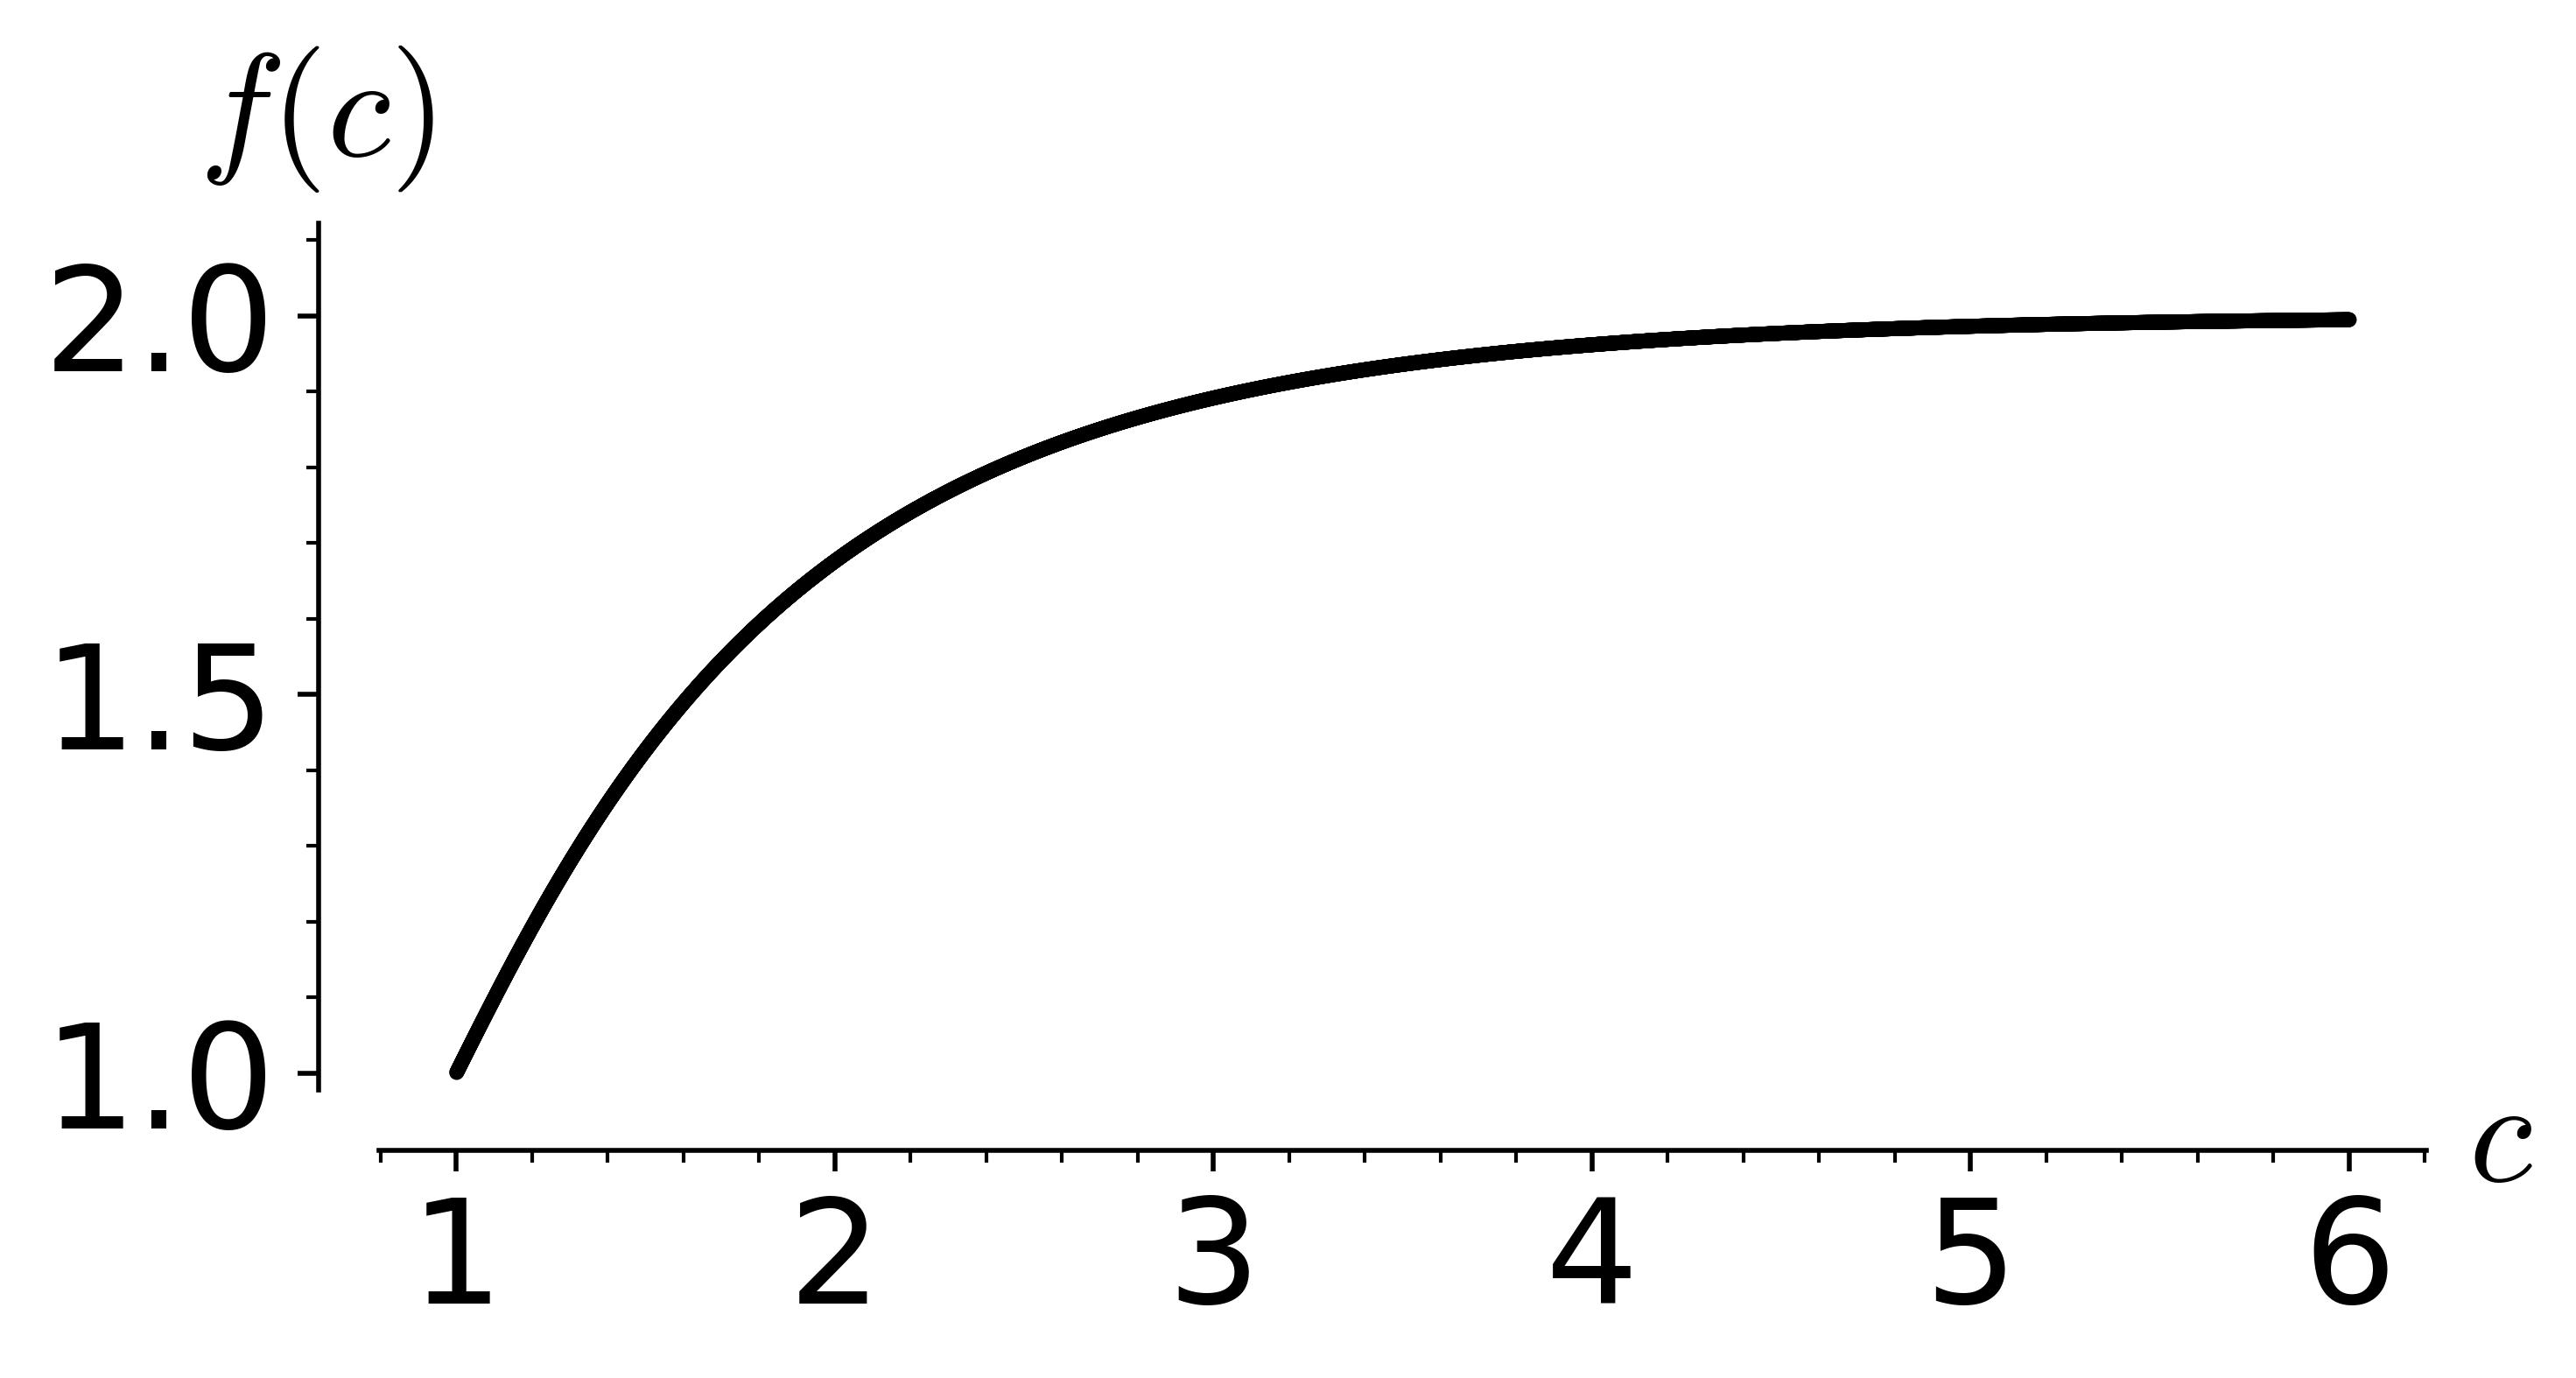
\includegraphics[scale=0.33]{process-function.png}
	\caption{The function $f$ as defined in \Cref{PPdef:func}.}
	\label{PPfig:function}
\end{figure}


%--- BIBLIOGRAPHY --------------------------------------------------------------

% Print bibliography and include it in the table of contents:
%\printbibliography[heading=bibintoc]
\bibliographystyle{abbrv}
\bibliography{phd-missethan}

\end{document}
